\PassOptionsToPackage{unicode=true}{hyperref} % options for packages loaded elsewhere
\PassOptionsToPackage{hyphens}{url}
%
\documentclass[
]{book}
\usepackage{lmodern}
\usepackage{amssymb,amsmath}
\usepackage{ifxetex,ifluatex}
\ifnum 0\ifxetex 1\fi\ifluatex 1\fi=0 % if pdftex
  \usepackage[T1]{fontenc}
  \usepackage[utf8]{inputenc}
  \usepackage{textcomp} % provides euro and other symbols
\else % if luatex or xelatex
  \usepackage{unicode-math}
  \defaultfontfeatures{Scale=MatchLowercase}
  \defaultfontfeatures[\rmfamily]{Ligatures=TeX,Scale=1}
\fi
% use upquote if available, for straight quotes in verbatim environments
\IfFileExists{upquote.sty}{\usepackage{upquote}}{}
\IfFileExists{microtype.sty}{% use microtype if available
  \usepackage[]{microtype}
  \UseMicrotypeSet[protrusion]{basicmath} % disable protrusion for tt fonts
}{}
\makeatletter
\@ifundefined{KOMAClassName}{% if non-KOMA class
  \IfFileExists{parskip.sty}{%
    \usepackage{parskip}
  }{% else
    \setlength{\parindent}{0pt}
    \setlength{\parskip}{6pt plus 2pt minus 1pt}}
}{% if KOMA class
  \KOMAoptions{parskip=half}}
\makeatother
\usepackage{xcolor}
\IfFileExists{xurl.sty}{\usepackage{xurl}}{} % add URL line breaks if available
\IfFileExists{bookmark.sty}{\usepackage{bookmark}}{\usepackage{hyperref}}
\hypersetup{
  pdftitle={Statistical Methods},
  pdfauthor={Post, Avery, Osborne},
  pdfborder={0 0 0},
  breaklinks=true}
\urlstyle{same}  % don't use monospace font for urls
\usepackage{color}
\usepackage{fancyvrb}
\newcommand{\VerbBar}{|}
\newcommand{\VERB}{\Verb[commandchars=\\\{\}]}
\DefineVerbatimEnvironment{Highlighting}{Verbatim}{commandchars=\\\{\}}
% Add ',fontsize=\small' for more characters per line
\usepackage{framed}
\definecolor{shadecolor}{RGB}{248,248,248}
\newenvironment{Shaded}{\begin{snugshade}}{\end{snugshade}}
\newcommand{\AlertTok}[1]{\textcolor[rgb]{0.94,0.16,0.16}{#1}}
\newcommand{\AnnotationTok}[1]{\textcolor[rgb]{0.56,0.35,0.01}{\textbf{\textit{#1}}}}
\newcommand{\AttributeTok}[1]{\textcolor[rgb]{0.77,0.63,0.00}{#1}}
\newcommand{\BaseNTok}[1]{\textcolor[rgb]{0.00,0.00,0.81}{#1}}
\newcommand{\BuiltInTok}[1]{#1}
\newcommand{\CharTok}[1]{\textcolor[rgb]{0.31,0.60,0.02}{#1}}
\newcommand{\CommentTok}[1]{\textcolor[rgb]{0.56,0.35,0.01}{\textit{#1}}}
\newcommand{\CommentVarTok}[1]{\textcolor[rgb]{0.56,0.35,0.01}{\textbf{\textit{#1}}}}
\newcommand{\ConstantTok}[1]{\textcolor[rgb]{0.00,0.00,0.00}{#1}}
\newcommand{\ControlFlowTok}[1]{\textcolor[rgb]{0.13,0.29,0.53}{\textbf{#1}}}
\newcommand{\DataTypeTok}[1]{\textcolor[rgb]{0.13,0.29,0.53}{#1}}
\newcommand{\DecValTok}[1]{\textcolor[rgb]{0.00,0.00,0.81}{#1}}
\newcommand{\DocumentationTok}[1]{\textcolor[rgb]{0.56,0.35,0.01}{\textbf{\textit{#1}}}}
\newcommand{\ErrorTok}[1]{\textcolor[rgb]{0.64,0.00,0.00}{\textbf{#1}}}
\newcommand{\ExtensionTok}[1]{#1}
\newcommand{\FloatTok}[1]{\textcolor[rgb]{0.00,0.00,0.81}{#1}}
\newcommand{\FunctionTok}[1]{\textcolor[rgb]{0.00,0.00,0.00}{#1}}
\newcommand{\ImportTok}[1]{#1}
\newcommand{\InformationTok}[1]{\textcolor[rgb]{0.56,0.35,0.01}{\textbf{\textit{#1}}}}
\newcommand{\KeywordTok}[1]{\textcolor[rgb]{0.13,0.29,0.53}{\textbf{#1}}}
\newcommand{\NormalTok}[1]{#1}
\newcommand{\OperatorTok}[1]{\textcolor[rgb]{0.81,0.36,0.00}{\textbf{#1}}}
\newcommand{\OtherTok}[1]{\textcolor[rgb]{0.56,0.35,0.01}{#1}}
\newcommand{\PreprocessorTok}[1]{\textcolor[rgb]{0.56,0.35,0.01}{\textit{#1}}}
\newcommand{\RegionMarkerTok}[1]{#1}
\newcommand{\SpecialCharTok}[1]{\textcolor[rgb]{0.00,0.00,0.00}{#1}}
\newcommand{\SpecialStringTok}[1]{\textcolor[rgb]{0.31,0.60,0.02}{#1}}
\newcommand{\StringTok}[1]{\textcolor[rgb]{0.31,0.60,0.02}{#1}}
\newcommand{\VariableTok}[1]{\textcolor[rgb]{0.00,0.00,0.00}{#1}}
\newcommand{\VerbatimStringTok}[1]{\textcolor[rgb]{0.31,0.60,0.02}{#1}}
\newcommand{\WarningTok}[1]{\textcolor[rgb]{0.56,0.35,0.01}{\textbf{\textit{#1}}}}
\usepackage{longtable,booktabs}
% Allow footnotes in longtable head/foot
\IfFileExists{footnotehyper.sty}{\usepackage{footnotehyper}}{\usepackage{footnote}}
\makesavenoteenv{longtable}
\usepackage{graphicx,grffile}
\makeatletter
\def\maxwidth{\ifdim\Gin@nat@width>\linewidth\linewidth\else\Gin@nat@width\fi}
\def\maxheight{\ifdim\Gin@nat@height>\textheight\textheight\else\Gin@nat@height\fi}
\makeatother
% Scale images if necessary, so that they will not overflow the page
% margins by default, and it is still possible to overwrite the defaults
% using explicit options in \includegraphics[width, height, ...]{}
\setkeys{Gin}{width=\maxwidth,height=\maxheight,keepaspectratio}
\setlength{\emergencystretch}{3em}  % prevent overfull lines
\providecommand{\tightlist}{%
  \setlength{\itemsep}{0pt}\setlength{\parskip}{0pt}}
\setcounter{secnumdepth}{5}
% Redefines (sub)paragraphs to behave more like sections
\ifx\paragraph\undefined\else
  \let\oldparagraph\paragraph
  \renewcommand{\paragraph}[1]{\oldparagraph{#1}\mbox{}}
\fi
\ifx\subparagraph\undefined\else
  \let\oldsubparagraph\subparagraph
  \renewcommand{\subparagraph}[1]{\oldsubparagraph{#1}\mbox{}}
\fi

% set default figure placement to htbp
\makeatletter
\def\fps@figure{htbp}
\makeatother

\usepackage{booktabs}
\usepackage[]{natbib}
\bibliographystyle{apalike}

\title{Statistical Methods}
\author{Post, Avery, Osborne}
\date{2020-04-07}

\usepackage{amsthm}
\newtheorem{theorem}{Theorem}[chapter]
\newtheorem{lemma}{Lemma}[chapter]
\newtheorem{corollary}{Corollary}[chapter]
\newtheorem{proposition}{Proposition}[chapter]
\newtheorem{conjecture}{Conjecture}[chapter]
\theoremstyle{definition}
\newtheorem{definition}{Definition}[chapter]
\theoremstyle{definition}
\newtheorem{example}{Example}[chapter]
\theoremstyle{definition}
\newtheorem{exercise}{Exercise}[chapter]
\theoremstyle{remark}
\newtheorem*{remark}{Remark}
\newtheorem*{solution}{Solution}
\let\BeginKnitrBlock\begin \let\EndKnitrBlock\end
\begin{document}
\maketitle

{
\setcounter{tocdepth}{1}
\tableofcontents
}
\hypertarget{introduction}{%
\chapter{Introduction}\label{introduction}}

\hypertarget{about-the-book}{%
\section{About the book}\label{about-the-book}}

The goal in creating this book is to provide a thorough treatment of applied statistical methodologies geared toward analyzing designed experiments. Our approach emphasizes the problems researchers encounter rather than providing a litany of solutions with only modest context. We discuss a real scientific problem, thoughtfully consider the data that could be used to answer that problem, investigate experimental designs that would be useful, and pursue statistical models to make informed decisions in the context of how the data was collected. The focus of the book is on the statistical modeling portion but problems are viewed holistically. We purposefully introduce the linear model framework in matrix form early on and place most of the methodologies under that umbrella. This helps the reader to see the methods as a part of a general framework as opposed to a set of tools within a toolbox. We believe that the book should be appropriate for a graduate level student that has some comfort in mathematics, particularly linear algebra. Both SAS and R are used throughout to make sure the book works for a wide audience of practitioners.

\hypertarget{software}{%
\section{Software}\label{software}}

At this point, software is a requirement for statistics in practice. There are many available software solutions ranging from point and click to full on programming. We've decided to focus on R and SAS for this book.

\begin{itemize}
\item
  R is an open source, platform agnostic, software that is widely used by statisticians. We'll use the RStudio interactive development environment to write and execute our R code.
\item
  SAS requires a license but is an extremely powerful software for doing modeling and is used widely enough to merit inclusion here. For those without a license, SAS University Edition can be installed for free and is also platform agnostic. We'll use the SAS Studio environment that comes with University Edition.
\end{itemize}

As we progress through the book we'll include graphs, descriptive statistics, and analyses from R and/or SAS. At the end of each chapter a section explaining how to create these in both R and SAS is included. The following sections give a brief introduction to each software that should prepare you for what's ahead!

You'll also notice a certain style to the way our code is written. Good programming practices (GPPs) are essential for improving productivity and collaborating with others - including future you! There are a lot of guidelines and resources about GPPs available. We'll cover just a few of the essentials here.

\begin{itemize}
\item
  Include a header at the top of the program that gives the author, date, and purpose of the program.
\item
  Place comments throughout the program explaining the purpose of different chunks of code as well as your thought process.
\item
  Spacing and indentation should be used throughout for readability of the program.
\item
  Group sections of your code that serve a certain purpose together.
\item
  Use a consistent naming scheme such as camelCase or underscores\_between\_words.
\end{itemize}

Many of these and other GPPs can be taken care of by programming in a notebook environment such as JUPYTER (which can include SAS) or R Markdown. Also using a version control software such as Git and Github is really useful!

\hypertarget{r}{%
\section{R}\label{r}}

The general workflow for programming in R involves taking raw data and importing it into R. Once that data is imported we often create numerical and graphical summaries of the data. The appropriate model or statistical method is then applied.

\begin{center}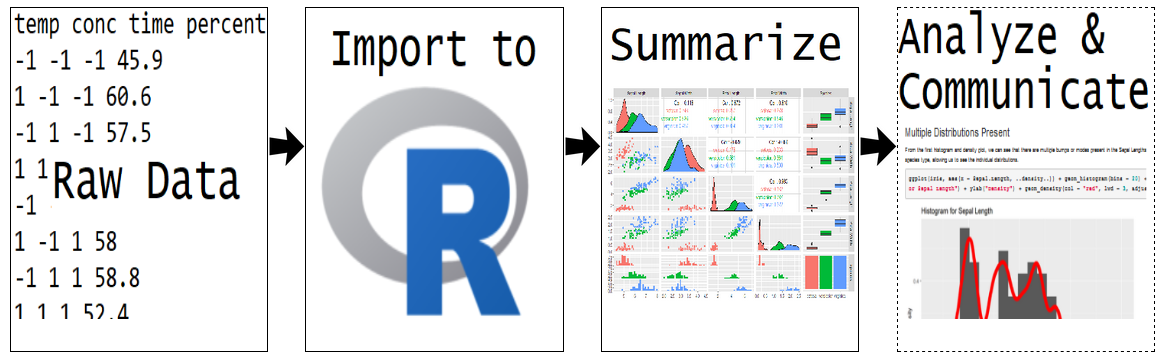
\includegraphics[width=0.8\linewidth]{img/RWorkFlow} \end{center}

At the end of this section the reader should be able to do the following:

\begin{itemize}
\tightlist
\item
  install R and RStudio\\
\item
  read and write basic R programs\\
\item
  import well-formatted data into R
\item
  do basic data manipulation in R
\end{itemize}

As the book progresses the steps of summarizing and analyzing the data will be covered. Let's get started!

\hypertarget{installing-r-and-rstudio}{%
\subsection{Installing R and RStudio}\label{installing-r-and-rstudio}}

The R software itself can be downloaded and installed by visiting the \href{https://cran.r-project.org/}{Comprehensive R Archive Network (Cran) website}. Here there are links to install R for Linux, Mac, and Windows-based machines.

\begin{itemize}
\item
  For Windows users, follow the initial `Download R for Windows' link and then click `install R for the first time.' From here you should now see a Download R X.x.x for Windows link that will download a .exe file. Once downloaded run that file and follow the prompts.
\item
  For Mac users, follow the initial `Download R for (Mac) OS X' link and click on the link near the `Latest Release' section similar to R-x.x.x.pkg. Once downloaded, you should be able to install by double clicking on the file.
\item
  For Linux users, follow the initial `Download R for Linux' link. Choose your OS and instructions are given on how to download R.
\end{itemize}

Once you've installed R you'll want to install RStudio. RStudio is a well-developed environment that makes programming in R much easier! To download head to \href{https://rstudio.com/products/rstudio/download/}{RStudio's download page}. From here choose RStudio Desktop (Open Source License) and a page with appropriate links to install are provided.

\hypertarget{using-rstudio}{%
\subsection{Using RStudio}\label{using-rstudio}}

To program in R you'll want to open RStudio. RStudio will submit R code for you so you never actually need to open R itself.

There are four main `areas' of the RStudio IDE:

\begin{itemize}
\item
  Console (\& Terminal)
\item
  Scripting and Viewing Window
\item
  Plots/Help (\& Files/Packages)
\item
  Environment (\& Connections/Git)
\end{itemize}

You may wish to rearrange the panes. This can be done via the menus at the top. Choose ``Tools --\textgreater{} Global Options''.

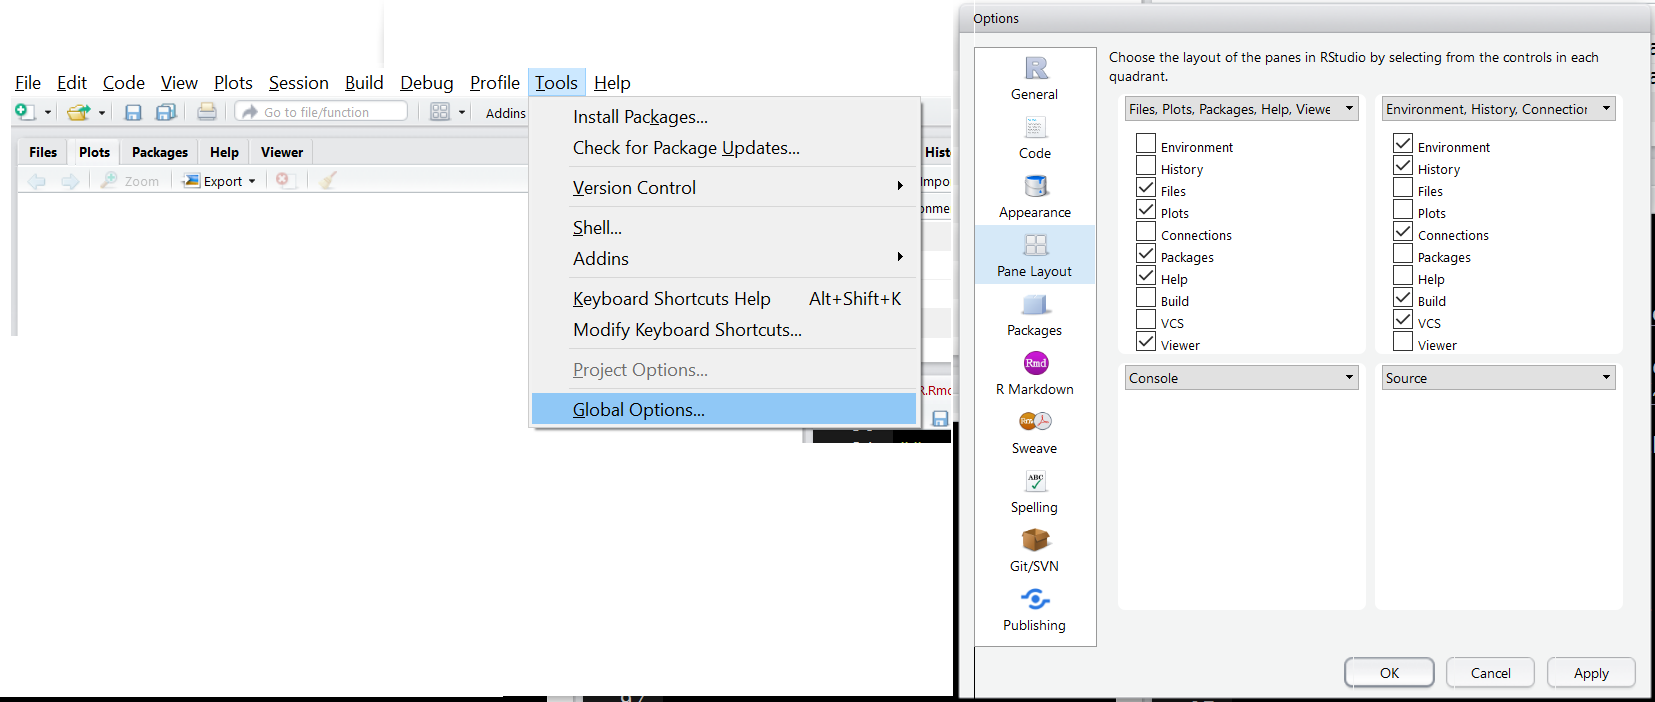
\includegraphics[width=0.8\linewidth]{img/panes}

Other useful global options to change are under the appearance tab (font size, theme) and under the code tab (editing --\textgreater{} soft-wrap, display --\textgreater{} show whitespace).

\hypertarget{console}{%
\subsubsection{Console}\label{console}}

To evaluate code you can type directly into the \textbf{console}.

\begin{Shaded}
\begin{Highlighting}[]
\CommentTok{#simple math operations}
\CommentTok{# <-- is a comment - code not evaluated}
\DecValTok{3} \OperatorTok{+}\StringTok{ }\DecValTok{7}
\end{Highlighting}
\end{Shaded}

\begin{verbatim}
## [1] 10
\end{verbatim}

\begin{Shaded}
\begin{Highlighting}[]
\DecValTok{10} \OperatorTok{*}\StringTok{ }\KeywordTok{exp}\NormalTok{(}\DecValTok{3}\NormalTok{) }\CommentTok{#exp is exponential function}
\end{Highlighting}
\end{Shaded}

\begin{verbatim}
## [1] 200.8554
\end{verbatim}

\begin{Shaded}
\begin{Highlighting}[]
\KeywordTok{log}\NormalTok{(pi}\OperatorTok{^}\DecValTok{2}\NormalTok{) }\CommentTok{#log is natural log by default}
\end{Highlighting}
\end{Shaded}

\begin{verbatim}
## [1] 2.28946
\end{verbatim}

\begin{Shaded}
\begin{Highlighting}[]
\KeywordTok{mean}\NormalTok{(cars}\OperatorTok{$}\NormalTok{speed)}
\end{Highlighting}
\end{Shaded}

\begin{verbatim}
## [1] 15.4
\end{verbatim}

\begin{Shaded}
\begin{Highlighting}[]
\KeywordTok{hist}\NormalTok{(cars}\OperatorTok{$}\NormalTok{speed)}
\end{Highlighting}
\end{Shaded}

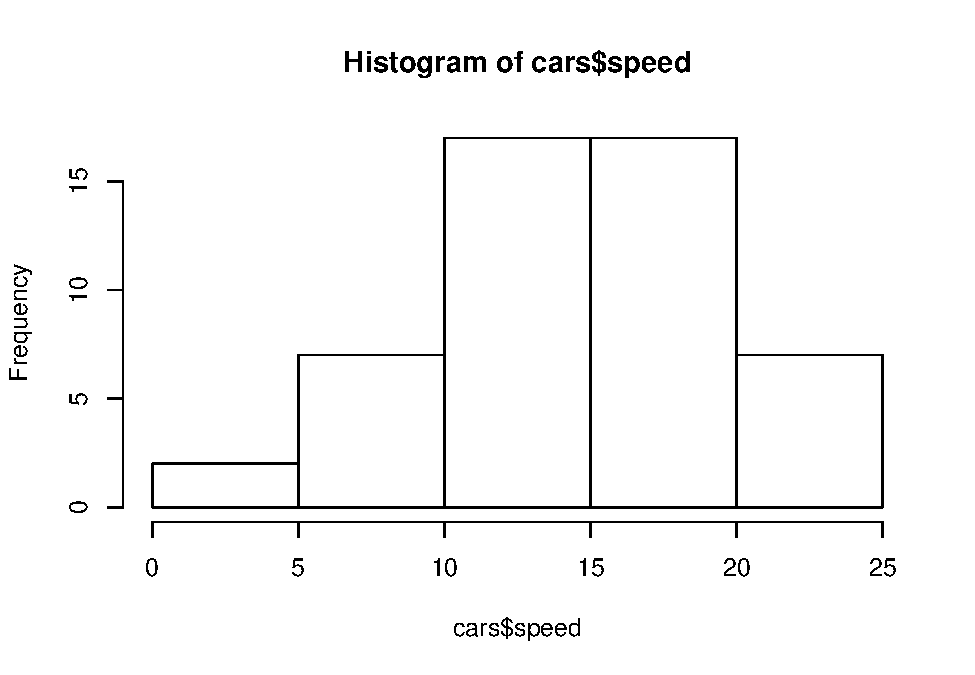
\includegraphics{StatisticalMethods_files/figure-latex/unnamed-chunk-190-1.pdf}

In the R sections of the book we spend much of our time learning the R syntax needed to create the appropriate summaries or analysis.

\hypertarget{scripting-and-viewing-window}{%
\subsubsection{Scripting and Viewing Window}\label{scripting-and-viewing-window}}

Usually you don't want to type code directly into the console because there isn't an easy way to get the code for later use. Instead code is usually written in an R `script' which is then saved.

From an R script you can send code to console via:

\begin{itemize}
\item
  ``Run'' button (runs current line)
\item
  CTRL+Enter (PC) or Command+Enter (MAC)
\item
  Highlight section and do above
\end{itemize}

To create a new R script you can use the menus at the top and go to File --\textgreater{} New File --\textgreater{} R Script. Take a moment and do this! Type the following into your script:

\begin{itemize}
\item
  \texttt{View(cars)} (note capital \texttt{V})
\item
  \texttt{plot(cars)}
\end{itemize}

Submit it to the console using a button or hot key!

\hypertarget{plotshelp}{%
\subsubsection{Plots/Help}\label{plotshelp}}

Created plots are stored in the \texttt{Plots} tab. This is a nice feature that allows you to cycle through past plots and easily save plots via menus.

In this pane there is also a \texttt{Help} tab that will enable you to learn about R functions. In the console type \texttt{help(hist)} for instance. Information about the \texttt{hist} function is presented. Being able to parse these types of help files is a really useful skill!

For every R function there are a few sections:

\begin{itemize}
\item
  Description - What the function is intended for.
\item
  Usage - How to call the function, inputs required, and which inputs have default arguments.

  \begin{itemize}
  \tightlist
  \item
    Here we see \texttt{hist(x,\ ...)}. This implies there is only one required input, \texttt{x}, and there is no default.\\
  \item
    Below you see a more detailed call to \texttt{hist} that includes other inputs. Each of these inputs has an equal sign with a value after it. This is the default value for that input (since there is a default value you don't have to specify it when you call). For instance, the \texttt{breaks\ =\ "Sturges"} input implies that the ``Sturges'' method is the default for determining how the bins of the histogram are created.
  \end{itemize}
\item
  Arguments - Describes the input requirements in more detail.
\item
  Details - Information about how the function works.
\item
  Values - Information about what is returned to the user.
\item
  References
\item
  See Also - Related functions.
\item
  Examples - Highly useful section giving code you can copy and paste to see an example of how the function can be used.
\end{itemize}

\hypertarget{environment}{%
\subsubsection{Environment}\label{environment}}

R stores \textbf{data/info/functions/etc.} in R objects. An object is a data structure having attributes and methods (more on this shortly). You can create an R object via \texttt{\textless{}-} (recommended) or \texttt{=}.

\begin{Shaded}
\begin{Highlighting}[]
\CommentTok{#save for later}
\NormalTok{avg <-}\StringTok{ }\NormalTok{(}\DecValTok{5} \OperatorTok{+}\StringTok{ }\DecValTok{7} \OperatorTok{+}\StringTok{ }\DecValTok{6}\NormalTok{) }\OperatorTok{/}\StringTok{ }\DecValTok{3}
\CommentTok{#call avg object}
\NormalTok{avg}
\end{Highlighting}
\end{Shaded}

\begin{verbatim}
## [1] 6
\end{verbatim}

\begin{Shaded}
\begin{Highlighting}[]
\CommentTok{#strings (text) can be saved as well}
\NormalTok{words <-}\StringTok{ }\KeywordTok{c}\NormalTok{(}\StringTok{"Hello there!"}\NormalTok{, }\StringTok{"How are you?"}\NormalTok{)}
\NormalTok{words}
\end{Highlighting}
\end{Shaded}

\begin{verbatim}
## [1] "Hello there!" "How are you?"
\end{verbatim}

Notice that when you send the line \texttt{avg\ \textless{}-\ (5+\ 7\ +\ 6)\ /\ 3} to the console (i.e.~create the object \texttt{avg}) that nothing prints out. This is common behavior when storing the object. The output or information is saved for later use in the object. To see the output or information you then simply call the object (a default printing method is used to display it).

You can look at all current objects with \texttt{ls()}.

\begin{Shaded}
\begin{Highlighting}[]
\KeywordTok{ls}\NormalTok{()}
\end{Highlighting}
\end{Shaded}

\begin{verbatim}
## [1] "avg"   "words"
\end{verbatim}

Use \texttt{rm()} to remove an object.

\begin{Shaded}
\begin{Highlighting}[]
\KeywordTok{rm}\NormalTok{(avg)}
\KeywordTok{ls}\NormalTok{()}
\end{Highlighting}
\end{Shaded}

\begin{verbatim}
## [1] "words"
\end{verbatim}

Built-in objects exist like \texttt{letters} and \texttt{cars}.

\begin{Shaded}
\begin{Highlighting}[]
\NormalTok{letters}
\end{Highlighting}
\end{Shaded}

\begin{verbatim}
##  [1] "a" "b" "c" "d" "e" "f" "g" "h" "i" "j" "k" "l" "m" "n" "o" "p" "q" "r" "s"
## [20] "t" "u" "v" "w" "x" "y" "z"
\end{verbatim}

\begin{Shaded}
\begin{Highlighting}[]
\KeywordTok{head}\NormalTok{(cars, }\DataTypeTok{n =} \DecValTok{3}\NormalTok{)}
\end{Highlighting}
\end{Shaded}

\begin{verbatim}
##   speed dist
## 1     4    2
## 2     4   10
## 3     7    4
\end{verbatim}

The function \texttt{data()} shows available built-in datasets.

You should now be roughly familiar with the four main `areas' of the RStudio IDE:

\begin{itemize}
\item
  Console (\& Terminal)
\item
  Scripting and Viewing Window
\item
  Plots/Help (\& Files/Packages)
\item
  Environment (\& Connections/Git)
\end{itemize}

\hypertarget{r-objects-and-classes}{%
\subsection{R Objects and Classes}\label{r-objects-and-classes}}

R has strong \textbf{O}bject \textbf{O}riented \textbf{P}rogramming (OOP) tools.

\begin{itemize}
\item
  Object: data structure with attributes (class)
\item
  Method: procedures (functions) that act on object based on attributes
\end{itemize}

R functions like \texttt{print()} or \texttt{plot()} act differently depending on an object's class.

\begin{Shaded}
\begin{Highlighting}[]
\KeywordTok{class}\NormalTok{(cars)}
\end{Highlighting}
\end{Shaded}

\begin{verbatim}
## [1] "data.frame"
\end{verbatim}

\begin{Shaded}
\begin{Highlighting}[]
\KeywordTok{plot}\NormalTok{(cars)}
\end{Highlighting}
\end{Shaded}

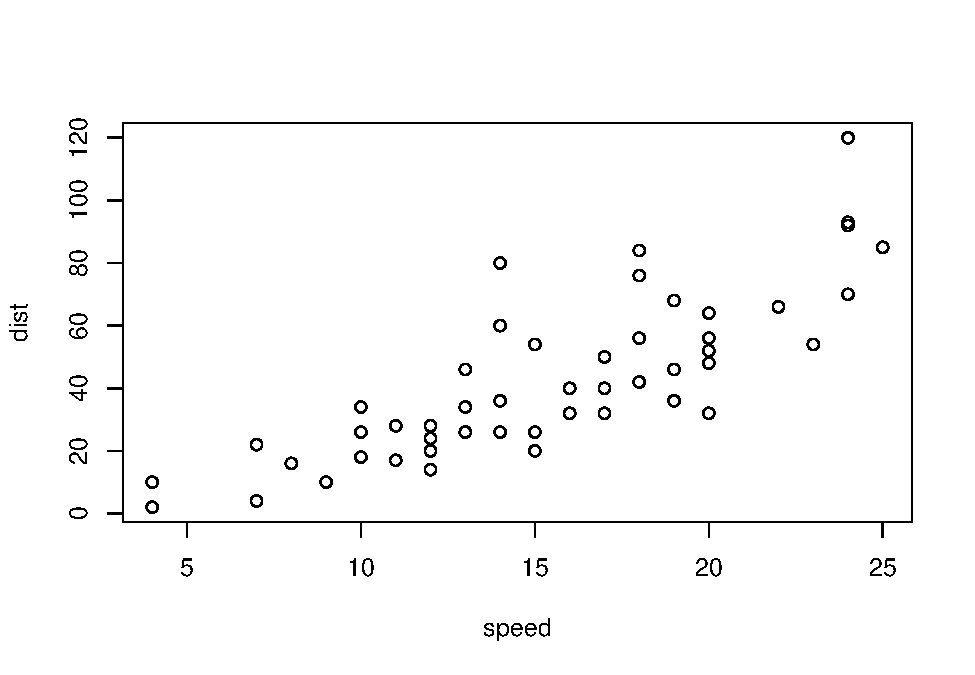
\includegraphics{StatisticalMethods_files/figure-latex/unnamed-chunk-195-1.pdf}

\begin{Shaded}
\begin{Highlighting}[]
\KeywordTok{class}\NormalTok{(exp)}
\end{Highlighting}
\end{Shaded}

\begin{verbatim}
## [1] "function"
\end{verbatim}

\begin{Shaded}
\begin{Highlighting}[]
\KeywordTok{plot}\NormalTok{(exp)}
\end{Highlighting}
\end{Shaded}

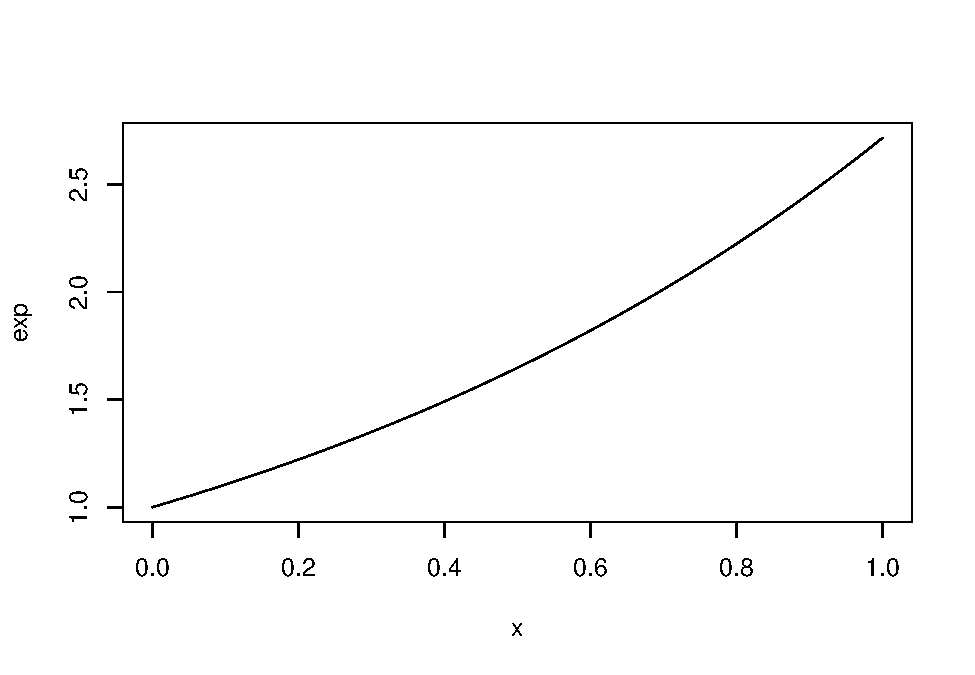
\includegraphics{StatisticalMethods_files/figure-latex/unnamed-chunk-195-2.pdf}

Many R functions exist to help understand an R Object.

\begin{itemize}
\tightlist
\item
  \texttt{str()} (structure)
\end{itemize}

\begin{Shaded}
\begin{Highlighting}[]
\KeywordTok{str}\NormalTok{(cars)}
\end{Highlighting}
\end{Shaded}

\begin{verbatim}
## 'data.frame':    50 obs. of  2 variables:
##  $ speed: num  4 4 7 7 8 9 10 10 10 11 ...
##  $ dist : num  2 10 4 22 16 10 18 26 34 17 ...
\end{verbatim}

\begin{itemize}
\tightlist
\item
  \texttt{class()}
\end{itemize}

\begin{Shaded}
\begin{Highlighting}[]
\KeywordTok{class}\NormalTok{(cars)}
\end{Highlighting}
\end{Shaded}

\begin{verbatim}
## [1] "data.frame"
\end{verbatim}

\begin{itemize}
\tightlist
\item
  \texttt{typeof()}
\end{itemize}

\begin{Shaded}
\begin{Highlighting}[]
\KeywordTok{typeof}\NormalTok{(cars)}
\end{Highlighting}
\end{Shaded}

\begin{verbatim}
## [1] "list"
\end{verbatim}

We'll use these functions later to help us know how to extra information from an R object.

Recall that we can create an R object via \texttt{\textless{}-} (recommended) or \texttt{=}. This allocates computer memory to object. The object's attributes depend on how you created it.

\begin{Shaded}
\begin{Highlighting}[]
\NormalTok{vec <-}\StringTok{ }\KeywordTok{c}\NormalTok{(}\DecValTok{1}\NormalTok{, }\DecValTok{4}\NormalTok{, }\DecValTok{10}\NormalTok{)}
\KeywordTok{class}\NormalTok{(vec)}
\end{Highlighting}
\end{Shaded}

\begin{verbatim}
## [1] "numeric"
\end{verbatim}

\begin{Shaded}
\begin{Highlighting}[]
\NormalTok{fit <-}\StringTok{ }\KeywordTok{lm}\NormalTok{(dist }\OperatorTok{~}\StringTok{ }\NormalTok{speed, }\DataTypeTok{data =}\NormalTok{ cars)}
\KeywordTok{class}\NormalTok{(fit)}
\end{Highlighting}
\end{Shaded}

\begin{verbatim}
## [1] "lm"
\end{verbatim}

\hypertarget{data-objects}{%
\subsection{Data Objects}\label{data-objects}}

To understand how to use R for data analysis we need to understand commonly used data structures:

\begin{verbatim}
 1. Atomic Vector (1D)  
 2. Matrix (2D)  
 3. Array (nd) (not covered)  
 4. Data Frame (2D)  
 5. List (1D)  
\end{verbatim}

\hypertarget{atomic-vector}{%
\subsubsection{Atomic Vector}\label{atomic-vector}}

Let's start with the most basic object and work our way up. An atomic vector is a 1D group of elements with an ordering.

\begin{center}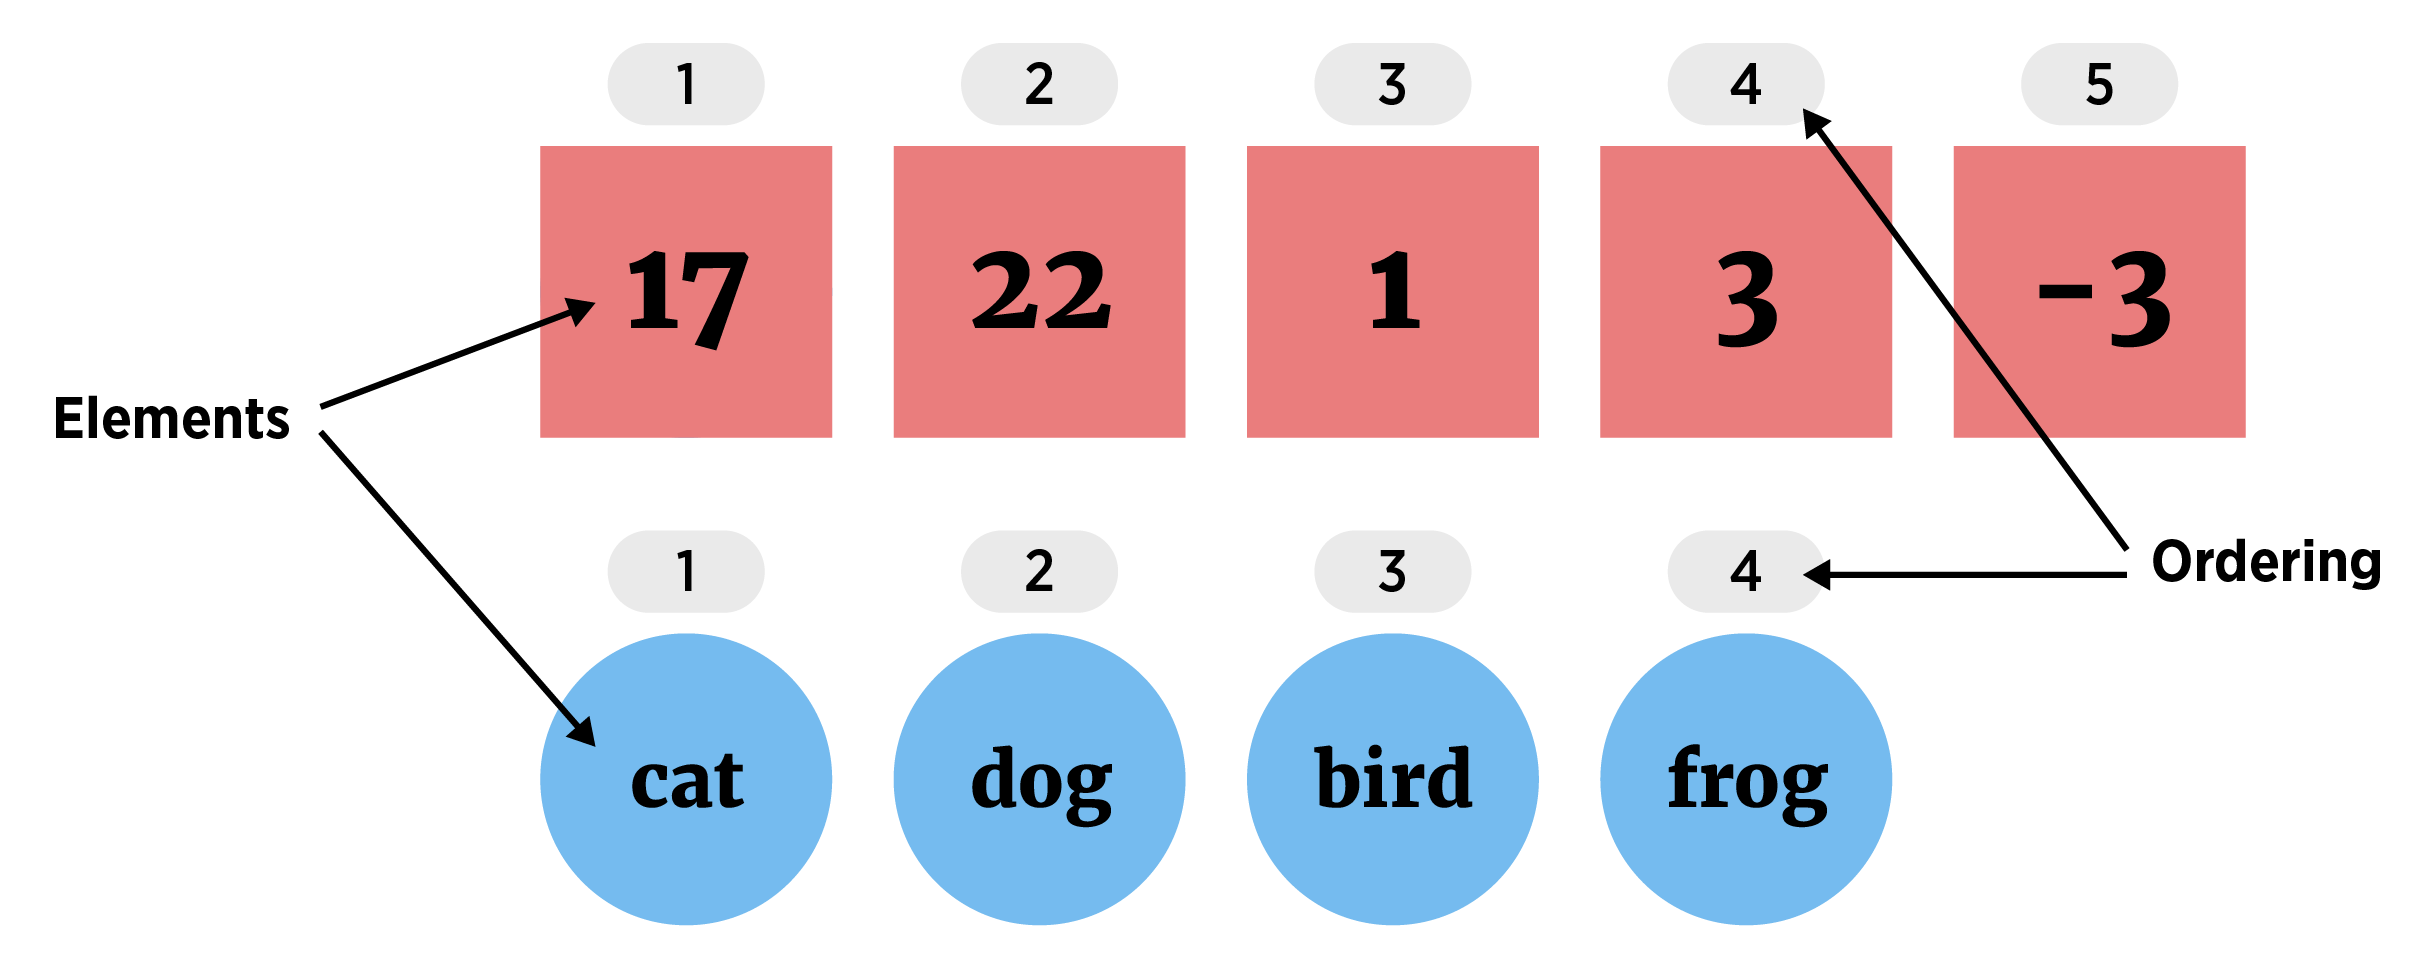
\includegraphics[width=0.8\linewidth]{img/vectorVisualF} \end{center}

All of the elements must be same `type'. Types include numeric (integer or double), character, or logical. We create an atomic vector with the \texttt{c()} function (`combine').

\begin{Shaded}
\begin{Highlighting}[]
\CommentTok{#vectors (1 dimensional) objects}
\NormalTok{x <-}\StringTok{ }\KeywordTok{c}\NormalTok{(}\DecValTok{17}\NormalTok{, }\DecValTok{22}\NormalTok{, }\DecValTok{1}\NormalTok{, }\DecValTok{3}\NormalTok{, }\DecValTok{-3}\NormalTok{)}
\NormalTok{y <-}\StringTok{ }\KeywordTok{c}\NormalTok{(}\StringTok{"cat"}\NormalTok{, }\StringTok{"dog"}\NormalTok{, }\StringTok{"bird"}\NormalTok{, }\StringTok{"frog"}\NormalTok{)}
\NormalTok{x}
\end{Highlighting}
\end{Shaded}

\begin{verbatim}
## [1] 17 22  1  3 -3
\end{verbatim}

\begin{Shaded}
\begin{Highlighting}[]
\NormalTok{y}
\end{Highlighting}
\end{Shaded}

\begin{verbatim}
## [1] "cat"  "dog"  "bird" "frog"
\end{verbatim}

In addition, many `functions' output a numeric vector. Functions are at the heart of R so it is vital to understand them. The concept of a function is that there the function takes an input or inputs and maps those inputs to some output(s).

\begin{center}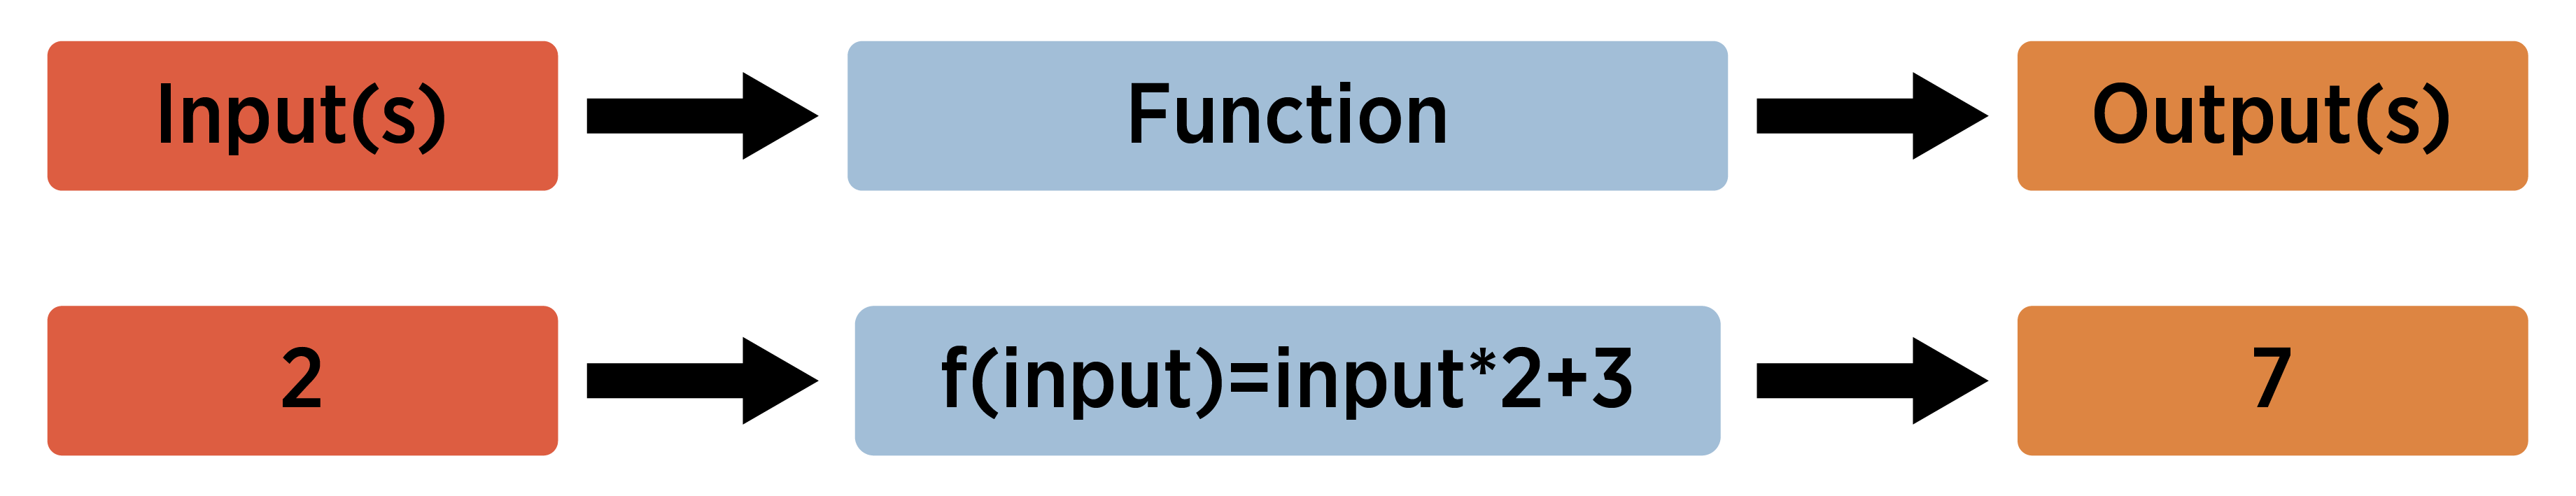
\includegraphics[width=0.8\linewidth]{img/funVisual1F} \end{center}

As an example, one function that outputs a numeric vector is the \texttt{seq} or sequence function. To know about a function you need to know about the inputs and ouputs. For \texttt{seq} we have the following:

\begin{verbatim}
+ Inputs = from, to, by (among others)  

+ Output = a sequence of numbers
\end{verbatim}

\begin{center}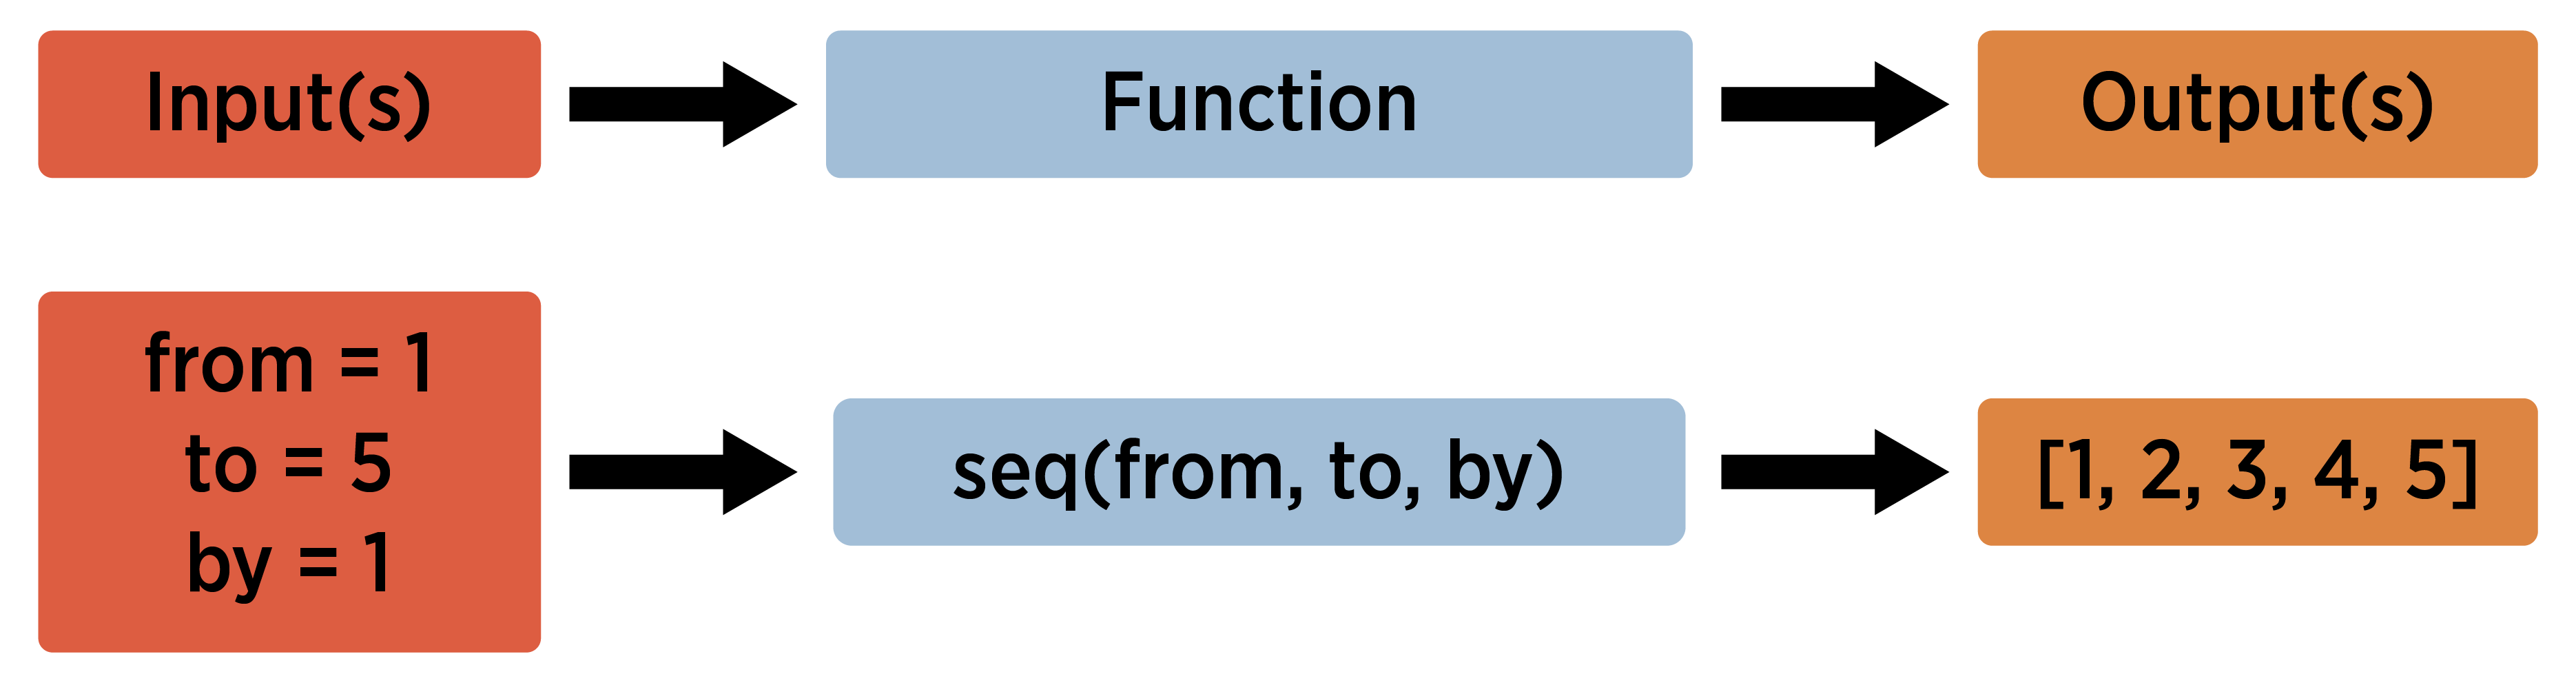
\includegraphics[width=0.8\linewidth]{img/funVisual2F} \end{center}

\begin{Shaded}
\begin{Highlighting}[]
\NormalTok{v <-}\StringTok{ }\KeywordTok{seq}\NormalTok{(}\DataTypeTok{from =} \DecValTok{1}\NormalTok{, }\DataTypeTok{to =} \DecValTok{5}\NormalTok{, }\DataTypeTok{by =} \DecValTok{1}\NormalTok{)}
\NormalTok{v}
\end{Highlighting}
\end{Shaded}

\begin{verbatim}
## [1] 1 2 3 4 5
\end{verbatim}

\begin{Shaded}
\begin{Highlighting}[]
\KeywordTok{str}\NormalTok{(v)}
\end{Highlighting}
\end{Shaded}

\begin{verbatim}
##  num [1:5] 1 2 3 4 5
\end{verbatim}

\texttt{str} tells about the object \texttt{v}:

\begin{itemize}
\item
  \texttt{num} says it is numeric
\item
  \texttt{{[}1:5{]}} implies one dimensional with elements 1, 2, 3, 4, 5
\end{itemize}

The \texttt{seq} function is used quite a bit. There is a shorthand way to create an integer sequence using \texttt{:}.

\begin{Shaded}
\begin{Highlighting}[]
\DecValTok{1}\OperatorTok{:}\DecValTok{20} 
\end{Highlighting}
\end{Shaded}

\begin{verbatim}
##  [1]  1  2  3  4  5  6  7  8  9 10 11 12 13 14 15 16 17 18 19 20
\end{verbatim}

It is also important to know how R does math on its objects. R does elementwise addition/subtraction and multiplication/division to vectors, matrices, and data frames. (The matrix multiplicaiton operator is \texttt{\%*\%}.).

\begin{Shaded}
\begin{Highlighting}[]
\DecValTok{1}\OperatorTok{:}\DecValTok{20}\OperatorTok{/}\DecValTok{20}
\end{Highlighting}
\end{Shaded}

\begin{verbatim}
##  [1] 0.05 0.10 0.15 0.20 0.25 0.30 0.35 0.40 0.45 0.50 0.55 0.60 0.65 0.70 0.75
## [16] 0.80 0.85 0.90 0.95 1.00
\end{verbatim}

\begin{Shaded}
\begin{Highlighting}[]
\DecValTok{1}\OperatorTok{:}\DecValTok{20} \OperatorTok{+}\StringTok{ }\DecValTok{1}
\end{Highlighting}
\end{Shaded}

\begin{verbatim}
##  [1]  2  3  4  5  6  7  8  9 10 11 12 13 14 15 16 17 18 19 20 21
\end{verbatim}

As we mentioned earlier, understanding help files is really useful to being about to program in R. As functions are ubiquitous in R we often need to learn about their inputs (or arguments) and we can do so using \texttt{help}.

To recap, our first commonly used R object for storing data is an atomic vectore. This is a 1D group of elements with an ordering where all of the elements are of the same type. Generally vectors are useful to know about but not usually useful for a storing a dataset exactly. They can often be considered as the `building blocks' for other data types.

\hypertarget{matrix}{%
\subsubsection{Matrix}\label{matrix}}

A Matrix is a 2D data structure in R whose elements are all of the same type. The first dimension refers to the rows and the second dimension refers to the columns. A 2D data object is very common. The rows often represent the \emph{observations} and the columns represent the \emph{variables}. Although not technically right, it is useful to think of the columns of a matrix as vectors of the same \textbf{type and length}.

\begin{center}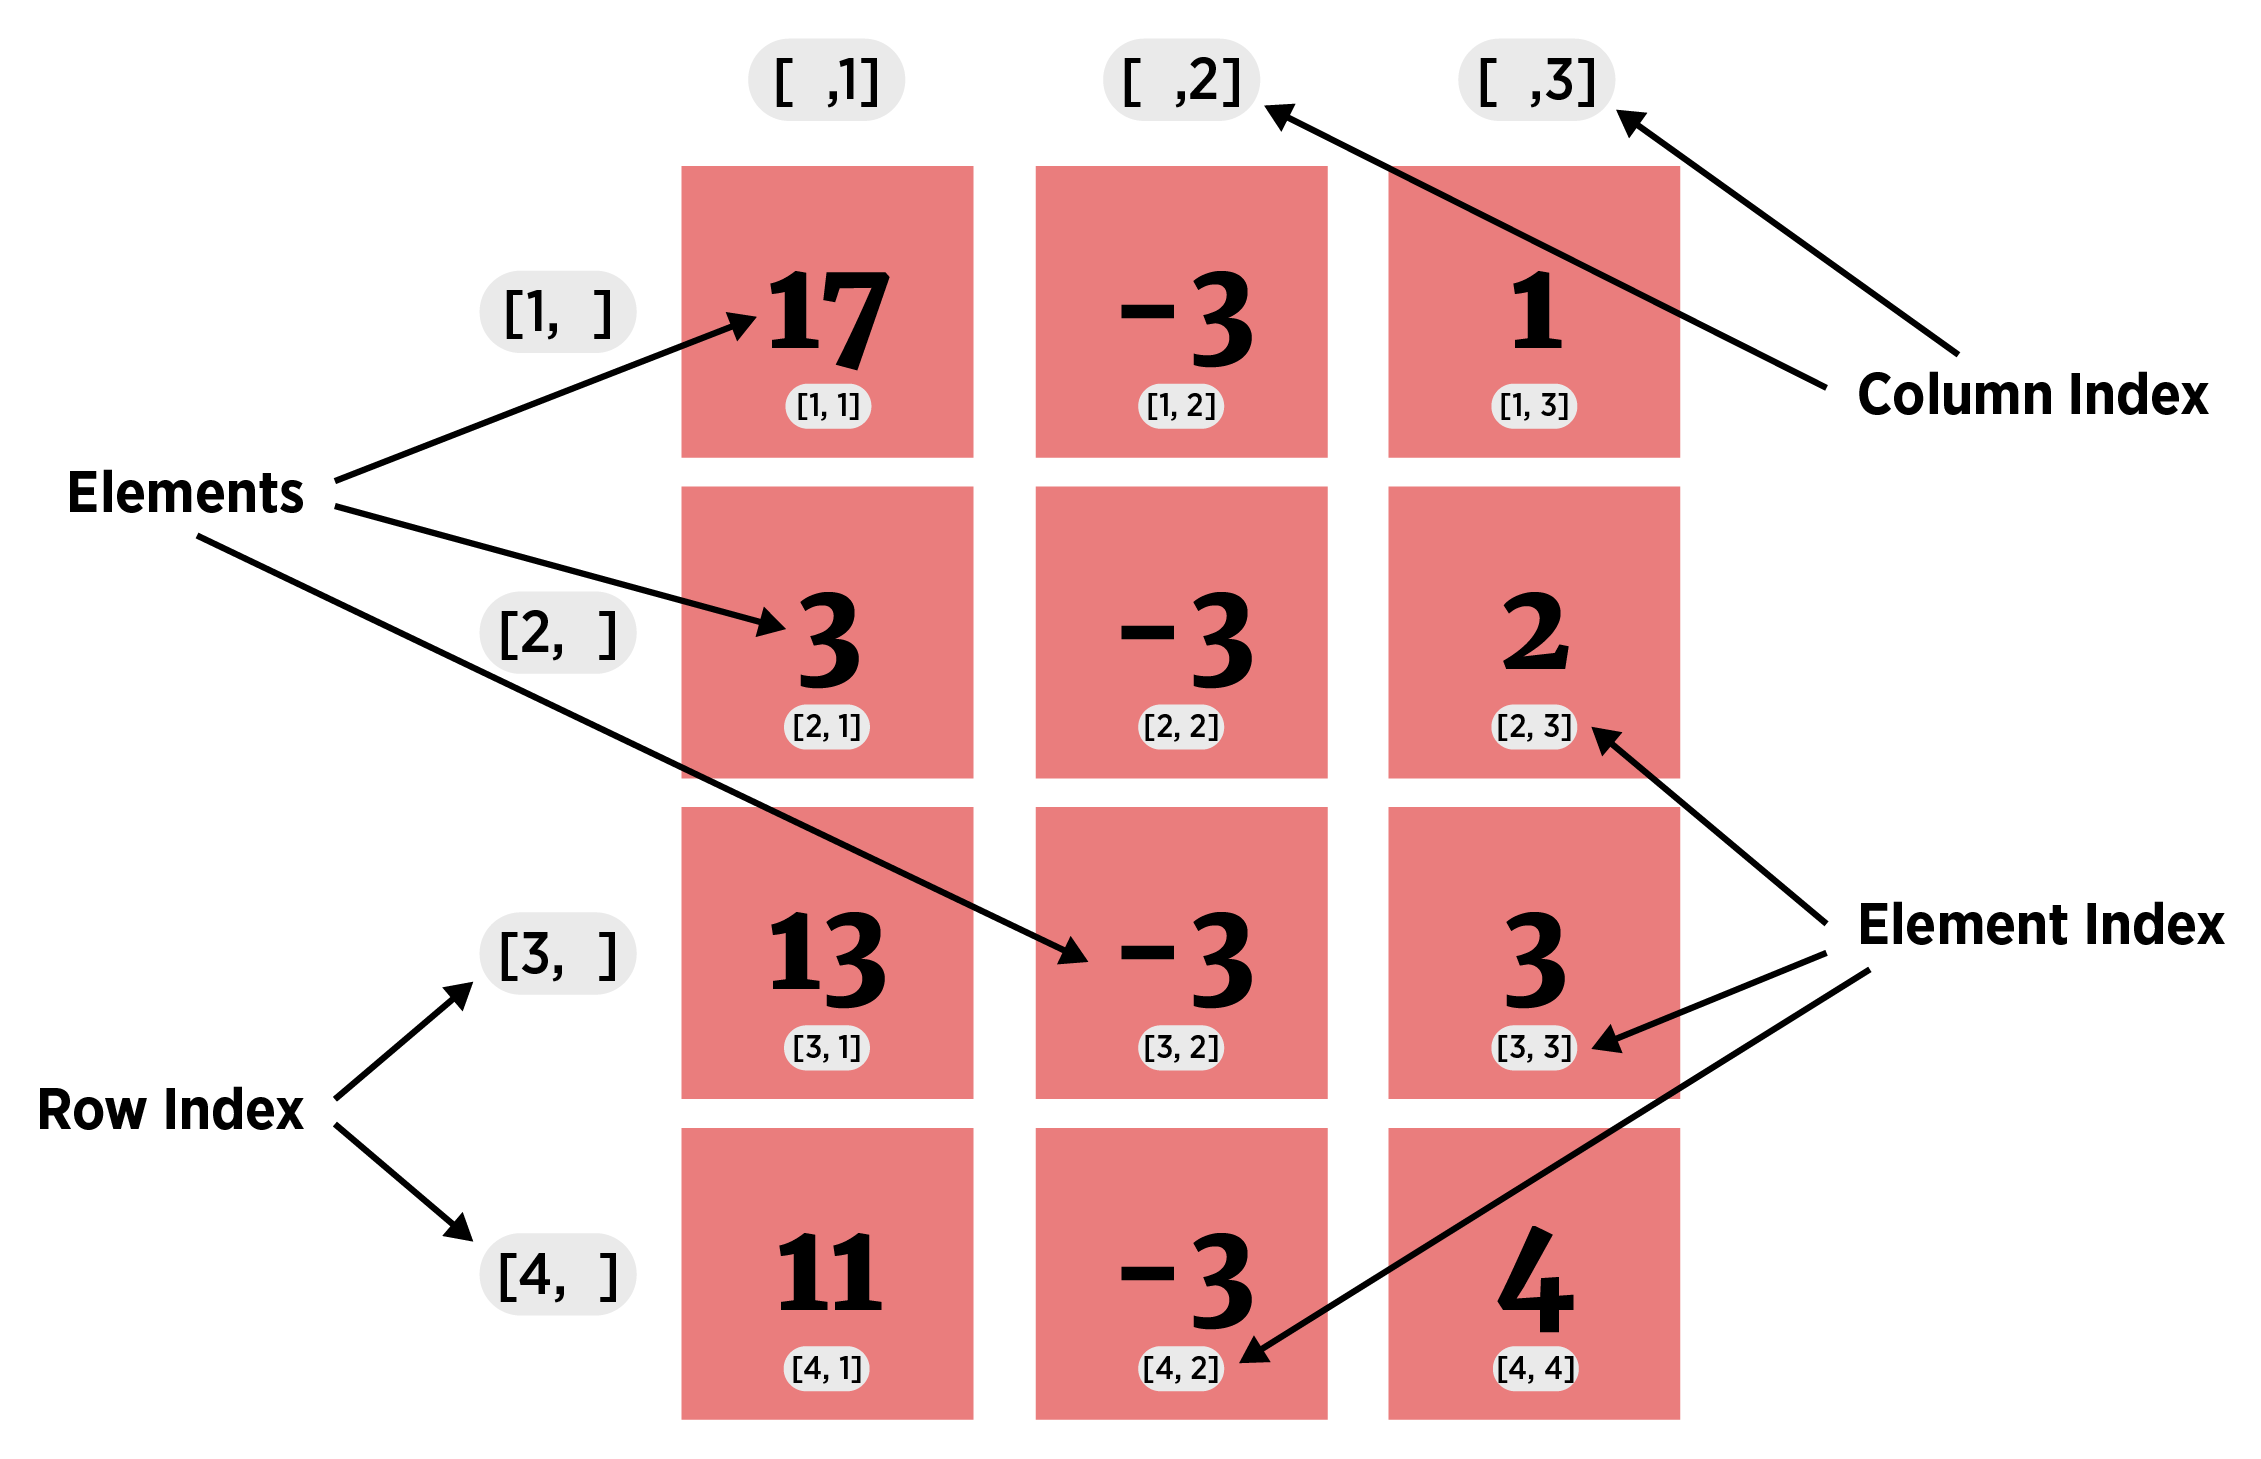
\includegraphics[width=0.75\linewidth]{img/matrixVisualF} \end{center}

For instance, consider the three vectors created here:

\begin{Shaded}
\begin{Highlighting}[]
\CommentTok{#populate vectors}
\NormalTok{x <-}\StringTok{ }\KeywordTok{c}\NormalTok{(}\DecValTok{17}\NormalTok{, }\DecValTok{3}\NormalTok{, }\DecValTok{13}\NormalTok{, }\DecValTok{11}\NormalTok{)}
\NormalTok{y <-}\StringTok{ }\KeywordTok{rep}\NormalTok{(}\OperatorTok{-}\DecValTok{3}\NormalTok{, }\DataTypeTok{times =} \DecValTok{4}\NormalTok{)}
\NormalTok{z <-}\StringTok{ }\DecValTok{1}\OperatorTok{:}\DecValTok{4}
\end{Highlighting}
\end{Shaded}

These are all of the same type. This can be checked with an \texttt{is.} (read as `is dot') function.

\begin{Shaded}
\begin{Highlighting}[]
\CommentTok{#check 'type'}
\KeywordTok{is.numeric}\NormalTok{(x)}
\end{Highlighting}
\end{Shaded}

\begin{verbatim}
## [1] TRUE
\end{verbatim}

\begin{Shaded}
\begin{Highlighting}[]
\KeywordTok{is.numeric}\NormalTok{(y)}
\end{Highlighting}
\end{Shaded}

\begin{verbatim}
## [1] TRUE
\end{verbatim}

\begin{Shaded}
\begin{Highlighting}[]
\KeywordTok{is.numeric}\NormalTok{(z)}
\end{Highlighting}
\end{Shaded}

\begin{verbatim}
## [1] TRUE
\end{verbatim}

Not only are these three objects the same type but they are also the same length. This can be checked using the \texttt{length} function.

\begin{Shaded}
\begin{Highlighting}[]
\CommentTok{#check 'length'}
\KeywordTok{length}\NormalTok{(x)}
\end{Highlighting}
\end{Shaded}

\begin{verbatim}
## [1] 4
\end{verbatim}

\begin{Shaded}
\begin{Highlighting}[]
\KeywordTok{length}\NormalTok{(y)}
\end{Highlighting}
\end{Shaded}

\begin{verbatim}
## [1] 4
\end{verbatim}

\begin{Shaded}
\begin{Highlighting}[]
\KeywordTok{length}\NormalTok{(z)}
\end{Highlighting}
\end{Shaded}

\begin{verbatim}
## [1] 4
\end{verbatim}

Again, it is useful to visualize the columns of a potential matrix as these vectors. We can create the matrix using the \texttt{matrix} function. The \texttt{matrix} function requires us to give the data as one vector. We can combine the \texttt{x}, \texttt{y}, and \texttt{z} objects into one vector using the \texttt{c} funciton. This is the first argument to the \texttt{matrix} function. The only other argument required is to either specify the number of rows (\texttt{nrow\ =}) or the number of columns (\texttt{ncol\ =}) (R will attempt to figure out the one that is not given using the total length of the specified data vector).

\begin{Shaded}
\begin{Highlighting}[]
\CommentTok{#combine in a matrix}
\KeywordTok{matrix}\NormalTok{(}\KeywordTok{c}\NormalTok{(x, y, z), }\DataTypeTok{ncol =} \DecValTok{3}\NormalTok{)}
\end{Highlighting}
\end{Shaded}

\begin{verbatim}
##      [,1] [,2] [,3]
## [1,]   17   -3    1
## [2,]    3   -3    2
## [3,]   13   -3    3
## [4,]   11   -3    4
\end{verbatim}

A matrix can also store character data as well. An example of this is given below and the number of rows is specified rather than the number of columns. Note the use of \texttt{is.character} from the \texttt{is.} family of functions.

\begin{Shaded}
\begin{Highlighting}[]
\NormalTok{x <-}\StringTok{ }\KeywordTok{c}\NormalTok{(}\StringTok{"Hi"}\NormalTok{, }\StringTok{"There"}\NormalTok{, }\StringTok{"!"}\NormalTok{)}
\NormalTok{y <-}\StringTok{ }\KeywordTok{c}\NormalTok{(}\StringTok{"a"}\NormalTok{, }\StringTok{"b"}\NormalTok{, }\StringTok{"c"}\NormalTok{)}
\NormalTok{z <-}\StringTok{ }\KeywordTok{c}\NormalTok{(}\StringTok{"One"}\NormalTok{, }\StringTok{"Two"}\NormalTok{, }\StringTok{"Three"}\NormalTok{)}
\KeywordTok{is.character}\NormalTok{(x)}
\end{Highlighting}
\end{Shaded}

\begin{verbatim}
## [1] TRUE
\end{verbatim}

\begin{Shaded}
\begin{Highlighting}[]
\KeywordTok{matrix}\NormalTok{(}\KeywordTok{c}\NormalTok{(x, y, z), }\DataTypeTok{nrow =} \DecValTok{3}\NormalTok{)}
\end{Highlighting}
\end{Shaded}

\begin{verbatim}
##      [,1]    [,2] [,3]   
## [1,] "Hi"    "a"  "One"  
## [2,] "There" "b"  "Two"  
## [3,] "!"     "c"  "Three"
\end{verbatim}

To recap, a Matrix is a 2D data structure where we can think of the columns as vectors of the same \textbf{type and length}. These are useful for some datasets but most datasets have some numeric and some character variables.

\begin{center}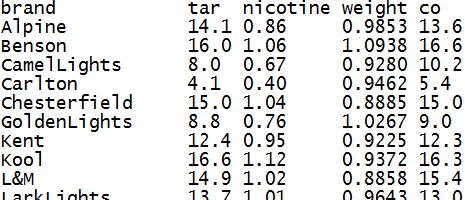
\includegraphics[width=0.8\linewidth]{img/dataset} \end{center}

Another 2D object called a data frame is perfect for this type of data!

\hypertarget{data-frame}{%
\subsubsection{Data Frame}\label{data-frame}}

A Data Frame is a 2D data structure where elements within a column must be of the same type but the columns themselves can differ in type. When thinking of a data frame, consider them as a collection (list) of vectors of the same \textbf{length}.

\begin{center}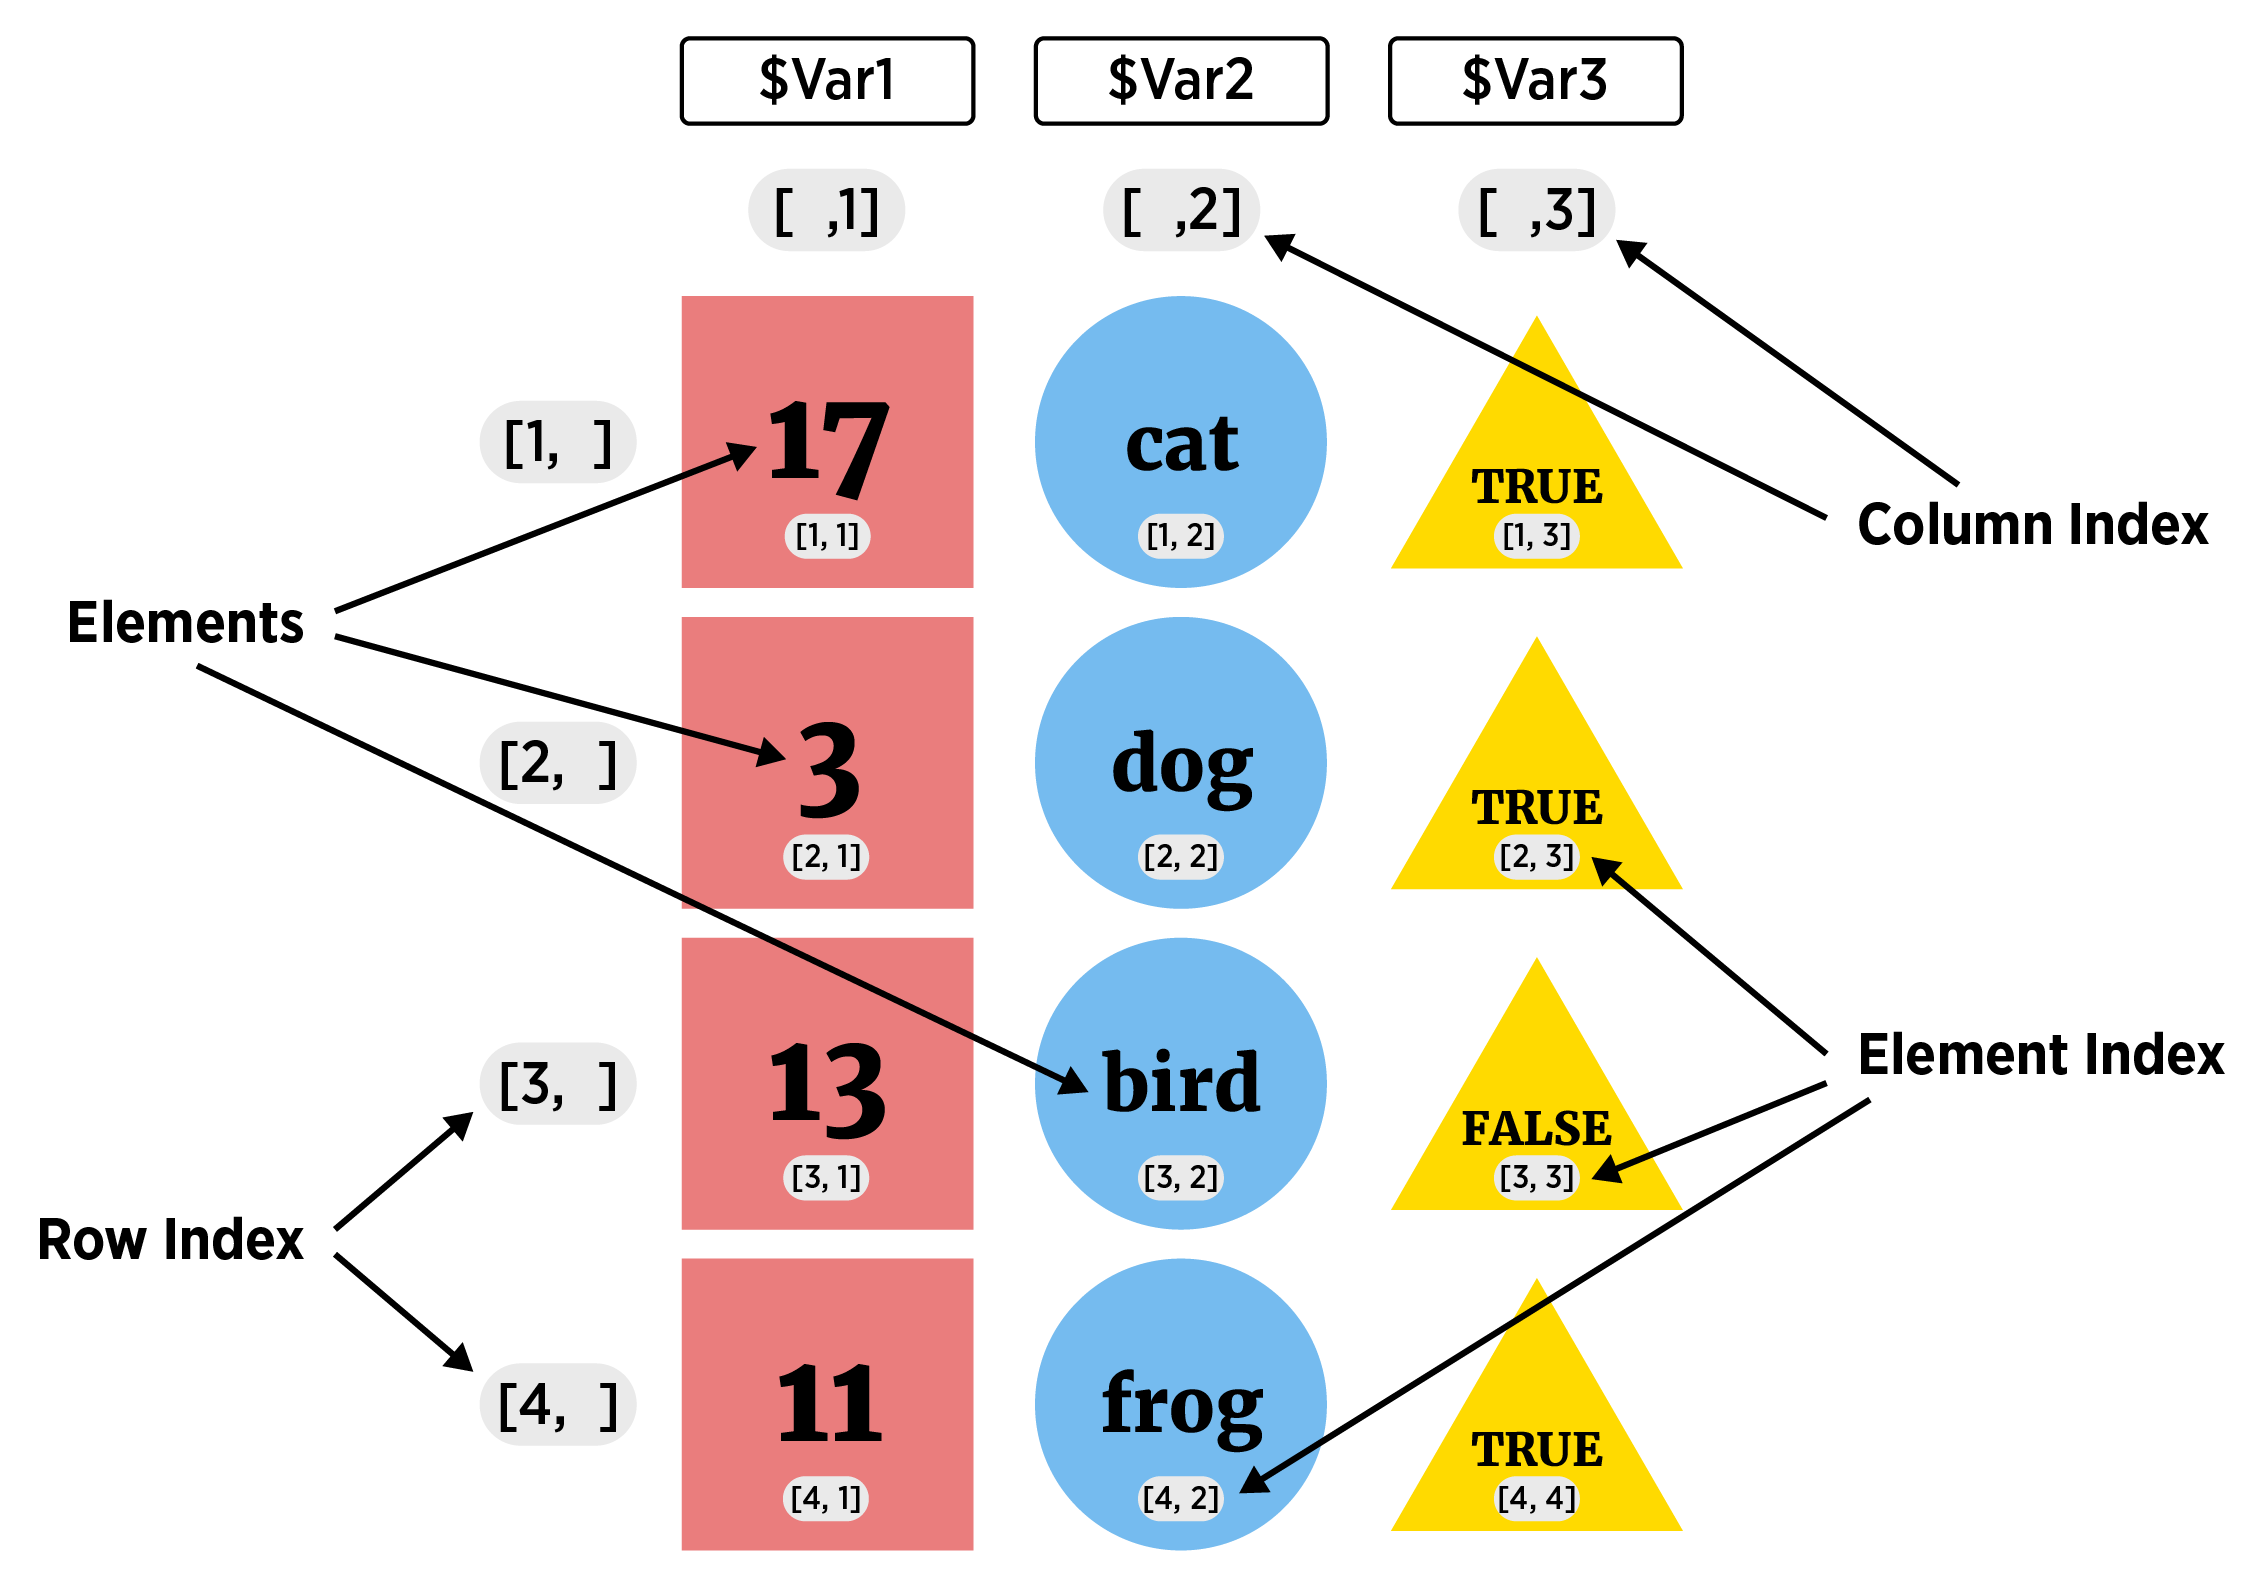
\includegraphics[width=0.8\linewidth]{img/dfVisualF} \end{center}

A data frame can be created with the \texttt{data.frame} function.

\begin{Shaded}
\begin{Highlighting}[]
\NormalTok{x <-}\StringTok{ }\KeywordTok{c}\NormalTok{(}\StringTok{"a"}\NormalTok{, }\StringTok{"b"}\NormalTok{, }\StringTok{"c"}\NormalTok{, }\StringTok{"d"}\NormalTok{, }\StringTok{"e"}\NormalTok{, }\StringTok{"f"}\NormalTok{)}
\NormalTok{y <-}\StringTok{ }\KeywordTok{c}\NormalTok{(}\DecValTok{1}\NormalTok{, }\DecValTok{3}\NormalTok{, }\DecValTok{4}\NormalTok{, }\DecValTok{-1}\NormalTok{, }\DecValTok{5}\NormalTok{, }\DecValTok{6}\NormalTok{)}
\NormalTok{z <-}\StringTok{ }\DecValTok{10}\OperatorTok{:}\DecValTok{15}
\KeywordTok{data.frame}\NormalTok{(x, y, z)}
\end{Highlighting}
\end{Shaded}

\begin{verbatim}
##   x  y  z
## 1 a  1 10
## 2 b  3 11
## 3 c  4 12
## 4 d -1 13
## 5 e  5 14
## 6 f  6 15
\end{verbatim}

You can also easily name the columns during creation.

\begin{Shaded}
\begin{Highlighting}[]
\KeywordTok{data.frame}\NormalTok{(}\DataTypeTok{char =}\NormalTok{ x, }\DataTypeTok{data1 =}\NormalTok{ y, }\DataTypeTok{data2 =}\NormalTok{ z)}
\end{Highlighting}
\end{Shaded}

\begin{verbatim}
##   char data1 data2
## 1    a     1    10
## 2    b     3    11
## 3    c     4    12
## 4    d    -1    13
## 5    e     5    14
## 6    f     6    15
\end{verbatim}

Notice that char, data1, and data2 become the variable names for the data frame.

To recap, consider a data frame as a collection (list) of vectors of the same \textbf{length}. Tis type of data structure is perfect for most data sets! Most functions that read 2D data into R store it as a data frame.

\hypertarget{list}{%
\subsubsection{List}\label{list}}

A List is a 1D group of objects with ordering. Really it is a vector that can have differing elements. Think of this in a similar way to the atomic vector previously discussed except the elements are really flexible.

\begin{center}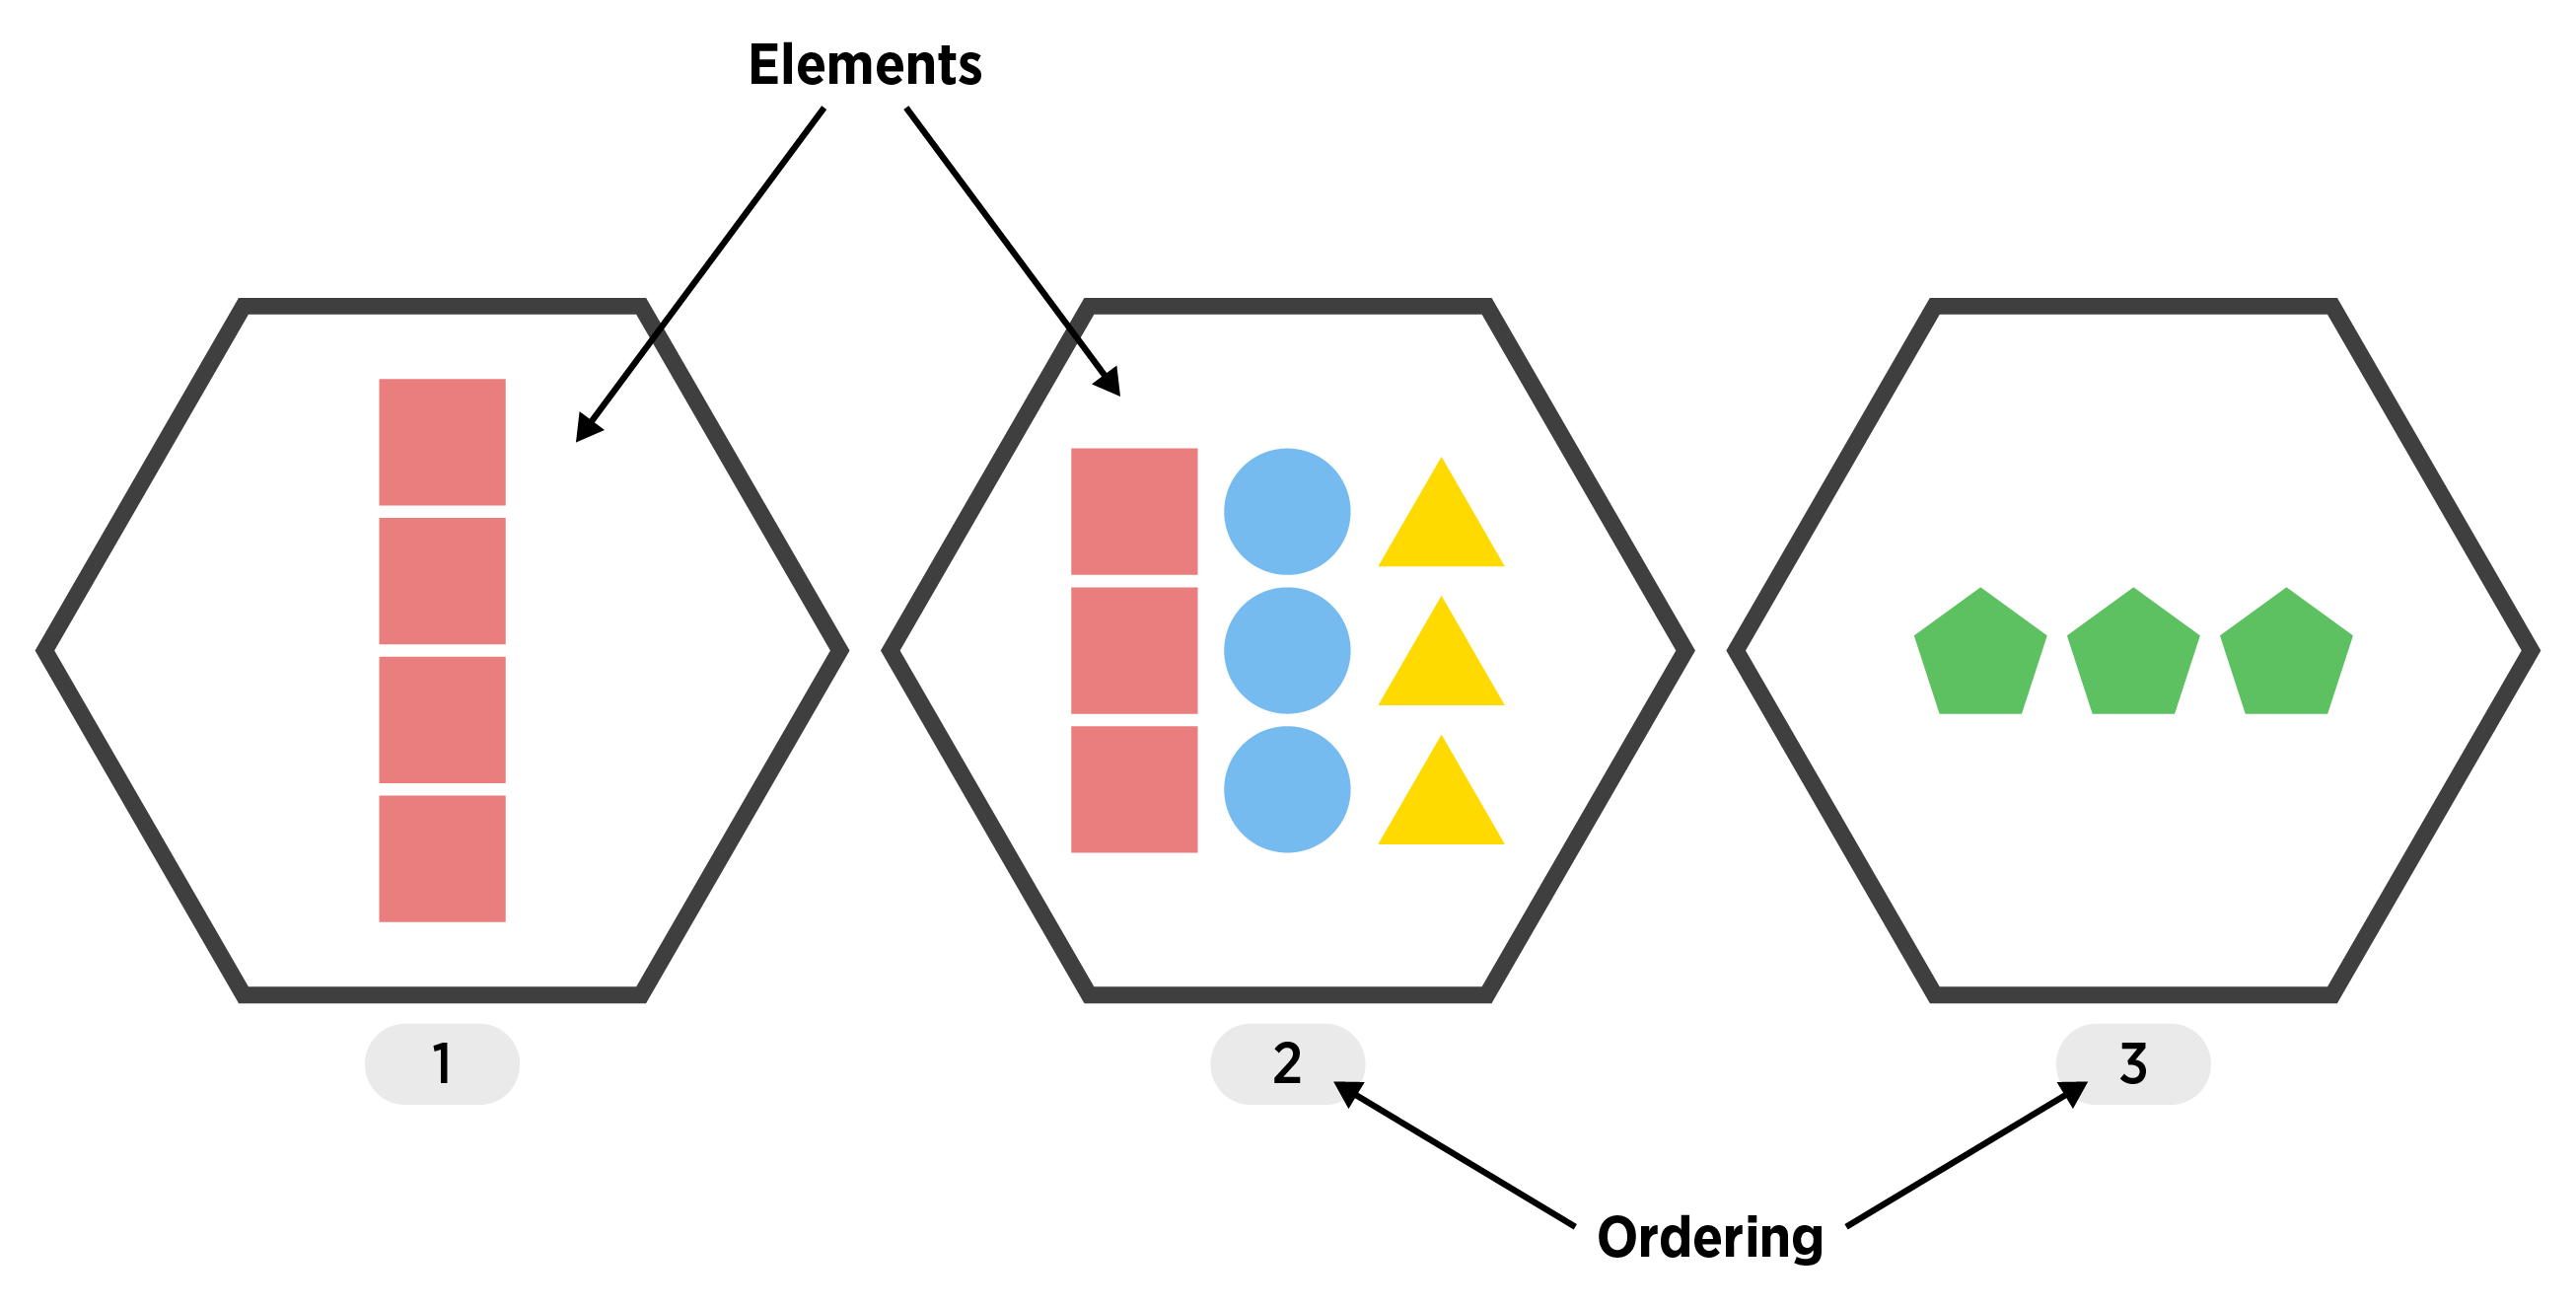
\includegraphics[width=0.8\linewidth]{img/listVisualF} \end{center}

A list can be created with the \texttt{list} function. You specify the elements you want to include, separated by commas.

\begin{Shaded}
\begin{Highlighting}[]
\KeywordTok{list}\NormalTok{(}\DecValTok{1}\OperatorTok{:}\DecValTok{3}\NormalTok{, }\KeywordTok{rnorm}\NormalTok{(}\DecValTok{2}\NormalTok{), }\KeywordTok{c}\NormalTok{(}\StringTok{"!"}\NormalTok{, }\StringTok{"?"}\NormalTok{))}
\end{Highlighting}
\end{Shaded}

\begin{verbatim}
## [[1]]
## [1] 1 2 3
## 
## [[2]]
## [1]  1.724243 -2.272354
## 
## [[3]]
## [1] "!" "?"
\end{verbatim}

Similar to a data frame, you can add names to the list elements during creation.

\begin{Shaded}
\begin{Highlighting}[]
\KeywordTok{list}\NormalTok{(}\DataTypeTok{seq =} \DecValTok{1}\OperatorTok{:}\DecValTok{3}\NormalTok{, }\DataTypeTok{normVals =} \KeywordTok{rnorm}\NormalTok{(}\DecValTok{2}\NormalTok{), }\DataTypeTok{punctuation =} \KeywordTok{c}\NormalTok{(}\StringTok{"!"}\NormalTok{, }\StringTok{"?"}\NormalTok{))}
\end{Highlighting}
\end{Shaded}

\begin{verbatim}
## $seq
## [1] 1 2 3
## 
## $normVals
## [1]  0.14407586 -0.02992154
## 
## $punctuation
## [1] "!" "?"
\end{verbatim}

To recap, a list is a very flexible 1D object. It is really useful for more complex types of data.

The table below gives a summary of the data objects we've covered. For most data analysis you'll use data frames.

\begin{longtable}[]{@{}lll@{}}
\toprule
Dimension & Homogeneous & Heterogeneous\tabularnewline
\midrule
\endhead
1d & Atomic Vector & List\tabularnewline
2d & Matrix & Data Frame\tabularnewline
\bottomrule
\end{longtable}

Next we look at how to access or change parts of our these common data objects.

\hypertarget{accessing-common-data-objects}{%
\subsection{Accessing Common Data Objects}\label{accessing-common-data-objects}}

When we are dealing with a data object (1D or 2D) we may want to extract a single element, certain columns, or certain rows. In this section we'll look at how to subset or extract information from each of the common data objects covered in the previous section.

\hypertarget{atomic-vector-1d}{%
\subsubsection{Atomic Vector (1D)}\label{atomic-vector-1d}}

For atomic vectors (and lists, see later) you can return elements using square brackets \texttt{{[}{]}}. You may notice that when R prints a vector to the console you often see \texttt{{[}1{]}} next to the first element and perhaps a \texttt{{[}\#{]}} where R has to break and move to the next line of the console. The \texttt{{[}1{]}} implies the element printed next is the first element of the vector (R starts its counting at 1 not 0 like some other languages). The \texttt{{[}\#{]}} implies that the element printed to the right is the \texttt{\#} element of the vector. This is a good reminder of how to extract values from an atomic vector.

As an example, here we extract from a built-in R object called letters that is a vector of length 26 containing the letters of the alphabet.

\begin{Shaded}
\begin{Highlighting}[]
\NormalTok{letters }\CommentTok{#built-in vector}
\end{Highlighting}
\end{Shaded}

\begin{verbatim}
##  [1] "a" "b" "c" "d" "e" "f" "g" "h" "i" "j" "k" "l" "m" "n" "o" "p" "q" "r" "s"
## [20] "t" "u" "v" "w" "x" "y" "z"
\end{verbatim}

\begin{Shaded}
\begin{Highlighting}[]
\NormalTok{letters[}\DecValTok{1}\NormalTok{] }\CommentTok{#R starts counting at 1!}
\end{Highlighting}
\end{Shaded}

\begin{verbatim}
## [1] "a"
\end{verbatim}

\begin{Shaded}
\begin{Highlighting}[]
\NormalTok{letters[}\DecValTok{26}\NormalTok{]}
\end{Highlighting}
\end{Shaded}

\begin{verbatim}
## [1] "z"
\end{verbatim}

To obtain more than one element you can `feed' in a vector of indices to that you'd like to return.

\begin{Shaded}
\begin{Highlighting}[]
\NormalTok{letters[}\DecValTok{1}\OperatorTok{:}\DecValTok{4}\NormalTok{]}
\end{Highlighting}
\end{Shaded}

\begin{verbatim}
## [1] "a" "b" "c" "d"
\end{verbatim}

\begin{Shaded}
\begin{Highlighting}[]
\NormalTok{letters[}\KeywordTok{c}\NormalTok{(}\DecValTok{5}\NormalTok{, }\DecValTok{10}\NormalTok{, }\DecValTok{15}\NormalTok{, }\DecValTok{20}\NormalTok{, }\DecValTok{25}\NormalTok{)]}
\end{Highlighting}
\end{Shaded}

\begin{verbatim}
## [1] "e" "j" "o" "t" "y"
\end{verbatim}

\begin{Shaded}
\begin{Highlighting}[]
\NormalTok{x <-}\StringTok{ }\KeywordTok{c}\NormalTok{(}\DecValTok{1}\NormalTok{, }\DecValTok{2}\NormalTok{, }\DecValTok{5}\NormalTok{)}
\NormalTok{letters[x]}
\end{Highlighting}
\end{Shaded}

\begin{verbatim}
## [1] "a" "b" "e"
\end{verbatim}

If you'd like to return all values except a certain subset, you can use negative indices.

\begin{Shaded}
\begin{Highlighting}[]
\NormalTok{letters[}\OperatorTok{-}\NormalTok{(}\DecValTok{1}\OperatorTok{:}\DecValTok{4}\NormalTok{)]}
\end{Highlighting}
\end{Shaded}

\begin{verbatim}
##  [1] "e" "f" "g" "h" "i" "j" "k" "l" "m" "n" "o" "p" "q" "r" "s" "t" "u" "v" "w"
## [20] "x" "y" "z"
\end{verbatim}

\begin{Shaded}
\begin{Highlighting}[]
\NormalTok{x <-}\StringTok{ }\KeywordTok{c}\NormalTok{(}\DecValTok{1}\NormalTok{, }\DecValTok{2}\NormalTok{, }\DecValTok{5}\NormalTok{)}
\NormalTok{letters[}\OperatorTok{-}\NormalTok{x]}
\end{Highlighting}
\end{Shaded}

\begin{verbatim}
##  [1] "c" "d" "f" "g" "h" "i" "j" "k" "l" "m" "n" "o" "p" "q" "r" "s" "t" "u" "v"
## [20] "w" "x" "y" "z"
\end{verbatim}

\hypertarget{matrices-2d}{%
\subsubsection{Matrices (2D)}\label{matrices-2d}}

For rectangular data like a matrix you can return rectangular subsets using square brackets with a comma \texttt{{[}\ ,\ {]}}. Notice default row and column names when R prints a matrix!

\begin{Shaded}
\begin{Highlighting}[]
\NormalTok{mat <-}\StringTok{ }\KeywordTok{matrix}\NormalTok{(}\KeywordTok{c}\NormalTok{(}\DecValTok{1}\OperatorTok{:}\DecValTok{4}\NormalTok{, }\DecValTok{20}\OperatorTok{:}\DecValTok{17}\NormalTok{), }\DataTypeTok{ncol =} \DecValTok{2}\NormalTok{)}
\NormalTok{mat}
\end{Highlighting}
\end{Shaded}

\begin{verbatim}
##      [,1] [,2]
## [1,]    1   20
## [2,]    2   19
## [3,]    3   18
## [4,]    4   17
\end{verbatim}

This is a nice reminder of how to index a matrix. The value prior to the columns represents which row(s) you want to return and the value after the comma which column(s). If an index is left blank then all of that corresponding dimension (row or column) is returned.

\begin{Shaded}
\begin{Highlighting}[]
\NormalTok{mat[}\KeywordTok{c}\NormalTok{(}\DecValTok{2}\NormalTok{, }\DecValTok{4}\NormalTok{), ]}
\end{Highlighting}
\end{Shaded}

\begin{verbatim}
##      [,1] [,2]
## [1,]    2   19
## [2,]    4   17
\end{verbatim}

\begin{Shaded}
\begin{Highlighting}[]
\NormalTok{mat[, }\DecValTok{1}\NormalTok{]}
\end{Highlighting}
\end{Shaded}

\begin{verbatim}
## [1] 1 2 3 4
\end{verbatim}

\begin{Shaded}
\begin{Highlighting}[]
\NormalTok{mat[}\DecValTok{2}\NormalTok{, ]}
\end{Highlighting}
\end{Shaded}

\begin{verbatim}
## [1]  2 19
\end{verbatim}

\begin{Shaded}
\begin{Highlighting}[]
\NormalTok{mat[}\DecValTok{2}\NormalTok{, }\DecValTok{1}\NormalTok{]}
\end{Highlighting}
\end{Shaded}

\begin{verbatim}
## [1] 2
\end{verbatim}

Notice that R simplifies the result where possible. That is, returns an atomic vector if you have only 1 dimension and a matrix if two. This can be changed by adding an additional argument to the \texttt{{[}} function.

\begin{Shaded}
\begin{Highlighting}[]
\NormalTok{mat[ , }\DecValTok{1}\NormalTok{, drop =}\StringTok{ }\OtherTok{FALSE}\NormalTok{]}
\end{Highlighting}
\end{Shaded}

\begin{verbatim}
##      [,1]
## [1,]    1
## [2,]    2
## [3,]    3
## [4,]    4
\end{verbatim}

Also, if you only give a single value in the \texttt{{[}{]}} then R uses the count of the value in the matrix. Counts go down columns first.

\begin{Shaded}
\begin{Highlighting}[]
\NormalTok{mat[}\DecValTok{5}\NormalTok{]}
\end{Highlighting}
\end{Shaded}

\begin{verbatim}
## [1] 20
\end{verbatim}

If your matrix has column names associated with it, you can also use those to return columns of interest. To add column names we can look run \texttt{help(matrix)} to learn how! Notice the \texttt{dimnames} argument. You can specify names for the rows and columns by using a list with two vectors. The first vector indicating row names and the second column names. If we don't want to give rownames we can give a NULL (a special value in R that is used for undefined values - here giving no specification of row names). We can do this and give a character vector for the column names.

\begin{Shaded}
\begin{Highlighting}[]
\NormalTok{mat<-}\KeywordTok{matrix}\NormalTok{(}\KeywordTok{c}\NormalTok{(}\DecValTok{1}\OperatorTok{:}\DecValTok{4}\NormalTok{, }\DecValTok{20}\OperatorTok{:}\DecValTok{17}\NormalTok{), }\DataTypeTok{ncol =} \DecValTok{2}\NormalTok{,}
            \DataTypeTok{dimnames =} \KeywordTok{list}\NormalTok{(}\OtherTok{NULL}\NormalTok{, }\KeywordTok{c}\NormalTok{(}\StringTok{"First"}\NormalTok{, }\StringTok{"Second"}\NormalTok{))}
\NormalTok{            )}
\NormalTok{mat}
\end{Highlighting}
\end{Shaded}

\begin{verbatim}
##      First Second
## [1,]     1     20
## [2,]     2     19
## [3,]     3     18
## [4,]     4     17
\end{verbatim}

Now we can request columns be using a single name or a character vector of names.

\begin{Shaded}
\begin{Highlighting}[]
\NormalTok{mat[, }\StringTok{"First"}\NormalTok{]}
\end{Highlighting}
\end{Shaded}

\begin{verbatim}
## [1] 1 2 3 4
\end{verbatim}

To return all but certain parts of a matrix you can still use negative indices but note that this won't work with column names.

\begin{Shaded}
\begin{Highlighting}[]
\NormalTok{mat[}\OperatorTok{-}\KeywordTok{c}\NormalTok{(}\DecValTok{1}\NormalTok{,}\DecValTok{3}\NormalTok{), }\OperatorTok{-}\StringTok{"First"}\NormalTok{]}
\end{Highlighting}
\end{Shaded}

\begin{verbatim}
## Error in -"First": invalid argument to unary operator
\end{verbatim}

\begin{Shaded}
\begin{Highlighting}[]
\NormalTok{mat[}\OperatorTok{-}\KeywordTok{c}\NormalTok{(}\DecValTok{1}\NormalTok{,}\DecValTok{3}\NormalTok{), }\StringTok{"First"}\NormalTok{]}
\end{Highlighting}
\end{Shaded}

\begin{verbatim}
## [1] 2 4
\end{verbatim}

\hypertarget{data-frames-2d}{%
\subsubsection{Data Frames (2D)}\label{data-frames-2d}}

Since a data frame is also a rectangular data object you can return rectangular subsets using square brackets with a comma \texttt{{[}\ ,\ {]}}!

As an example, we'll subset the built-in \texttt{iris} data frame. To get an idea about this object we can run \texttt{str(iris)}.

\begin{Shaded}
\begin{Highlighting}[]
\KeywordTok{str}\NormalTok{(iris)}
\end{Highlighting}
\end{Shaded}

\begin{verbatim}
## 'data.frame':    150 obs. of  5 variables:
##  $ Sepal.Length: num  5.1 4.9 4.7 4.6 5 5.4 4.6 5 4.4 4.9 ...
##  $ Sepal.Width : num  3.5 3 3.2 3.1 3.6 3.9 3.4 3.4 2.9 3.1 ...
##  $ Petal.Length: num  1.4 1.4 1.3 1.5 1.4 1.7 1.4 1.5 1.4 1.5 ...
##  $ Petal.Width : num  0.2 0.2 0.2 0.2 0.2 0.4 0.3 0.2 0.2 0.1 ...
##  $ Species     : Factor w/ 3 levels "setosa","versicolor",..: 1 1 1 1 1 1 1 1 1 1 ...
\end{verbatim}

We can see this is a data frame with a few columns, four are numeric and one is a factor (a special type of character vector essentially - these will be covered when we discuss plotting).

\begin{Shaded}
\begin{Highlighting}[]
\NormalTok{iris[}\DecValTok{1}\OperatorTok{:}\DecValTok{4}\NormalTok{, }\DecValTok{2}\OperatorTok{:}\DecValTok{4}\NormalTok{]}
\end{Highlighting}
\end{Shaded}

\begin{verbatim}
##   Sepal.Width Petal.Length Petal.Width
## 1         3.5          1.4         0.2
## 2         3.0          1.4         0.2
## 3         3.2          1.3         0.2
## 4         3.1          1.5         0.2
\end{verbatim}

\begin{Shaded}
\begin{Highlighting}[]
\NormalTok{iris[}\DecValTok{1}\NormalTok{, ]}
\end{Highlighting}
\end{Shaded}

\begin{verbatim}
##   Sepal.Length Sepal.Width Petal.Length Petal.Width Species
## 1          5.1         3.5          1.4         0.2  setosa
\end{verbatim}

\begin{Shaded}
\begin{Highlighting}[]
\NormalTok{iris[, }\DecValTok{1}\NormalTok{]}
\end{Highlighting}
\end{Shaded}

\begin{verbatim}
##   [1] 5.1 4.9 4.7 4.6 5.0 5.4 4.6 5.0 4.4 4.9 5.4 4.8 4.8 4.3 5.8 5.7 5.4 5.1
##  [19] 5.7 5.1 5.4 5.1 4.6 5.1 4.8 5.0 5.0 5.2 5.2 4.7 4.8 5.4 5.2 5.5 4.9 5.0
##  [37] 5.5 4.9 4.4 5.1 5.0 4.5 4.4 5.0 5.1 4.8 5.1 4.6 5.3 5.0 7.0 6.4 6.9 5.5
##  [55] 6.5 5.7 6.3 4.9 6.6 5.2 5.0 5.9 6.0 6.1 5.6 6.7 5.6 5.8 6.2 5.6 5.9 6.1
##  [73] 6.3 6.1 6.4 6.6 6.8 6.7 6.0 5.7 5.5 5.5 5.8 6.0 5.4 6.0 6.7 6.3 5.6 5.5
##  [91] 5.5 6.1 5.8 5.0 5.6 5.7 5.7 6.2 5.1 5.7
##  [ reached getOption("max.print") -- omitted 50 entries ]
\end{verbatim}

Notice the simplification done when a single column is selected. R will simplify to a vector unless \texttt{drop\ =\ FALSE} is included as done in the matrix section. (The simplification doesn't occur when a single row is selected because data frames are actually lists - we'll discuss this more in the list section!)

You can use columns names to subset as well.

\begin{Shaded}
\begin{Highlighting}[]
\NormalTok{iris[}\DecValTok{1}\OperatorTok{:}\DecValTok{10}\NormalTok{ , }\KeywordTok{c}\NormalTok{(}\StringTok{"Sepal.Length"}\NormalTok{, }\StringTok{"Species"}\NormalTok{)]}
\end{Highlighting}
\end{Shaded}

\begin{verbatim}
##    Sepal.Length Species
## 1           5.1  setosa
## 2           4.9  setosa
## 3           4.7  setosa
## 4           4.6  setosa
## 5           5.0  setosa
## 6           5.4  setosa
## 7           4.6  setosa
## 8           5.0  setosa
## 9           4.4  setosa
## 10          4.9  setosa
\end{verbatim}

The most common way to access a single columns is to use the dollar sign operator.

\begin{Shaded}
\begin{Highlighting}[]
\NormalTok{iris}\OperatorTok{$}\NormalTok{Sepal.Length}
\end{Highlighting}
\end{Shaded}

\begin{verbatim}
##   [1] 5.1 4.9 4.7 4.6 5.0 5.4 4.6 5.0 4.4 4.9 5.4 4.8 4.8 4.3 5.8 5.7 5.4 5.1
##  [19] 5.7 5.1 5.4 5.1 4.6 5.1 4.8 5.0 5.0 5.2 5.2 4.7 4.8 5.4 5.2 5.5 4.9 5.0
##  [37] 5.5 4.9 4.4 5.1 5.0 4.5 4.4 5.0 5.1 4.8 5.1 4.6 5.3 5.0 7.0 6.4 6.9 5.5
##  [55] 6.5 5.7 6.3 4.9 6.6 5.2 5.0 5.9 6.0 6.1 5.6 6.7 5.6 5.8 6.2 5.6 5.9 6.1
##  [73] 6.3 6.1 6.4 6.6 6.8 6.7 6.0 5.7 5.5 5.5 5.8 6.0 5.4 6.0 6.7 6.3 5.6 5.5
##  [91] 5.5 6.1 5.8 5.0 5.6 5.7 5.7 6.2 5.1 5.7
##  [ reached getOption("max.print") -- omitted 50 entries ]
\end{verbatim}

A nice benefit of using RStudio is that column names will be filled in automatically as you type. In your console do the following:

\begin{itemize}
\tightlist
\item
  Type \texttt{iris\$}\\
\item
  If no choices - hit tab
\item
  Scroll up and down or continue typing to highlight the column of interest\\
\item
  Hit tab again to choose
\end{itemize}

\hypertarget{lists-1d}{%
\subsubsection{Lists (1D)}\label{lists-1d}}

As a list is a 1D data object we can use single square brackets \texttt{{[}\ {]}} for multiple list elements.

\begin{Shaded}
\begin{Highlighting}[]
\NormalTok{x <-}\StringTok{ }\KeywordTok{list}\NormalTok{(}\StringTok{"HI"}\NormalTok{, }\KeywordTok{c}\NormalTok{(}\DecValTok{10}\OperatorTok{:}\DecValTok{20}\NormalTok{), }\DecValTok{1}\NormalTok{)}
\NormalTok{x}
\end{Highlighting}
\end{Shaded}

\begin{verbatim}
## [[1]]
## [1] "HI"
## 
## [[2]]
##  [1] 10 11 12 13 14 15 16 17 18 19 20
## 
## [[3]]
## [1] 1
\end{verbatim}

\begin{Shaded}
\begin{Highlighting}[]
\NormalTok{x[}\DecValTok{2}\OperatorTok{:}\DecValTok{3}\NormalTok{]}
\end{Highlighting}
\end{Shaded}

\begin{verbatim}
## [[1]]
##  [1] 10 11 12 13 14 15 16 17 18 19 20
## 
## [[2]]
## [1] 1
\end{verbatim}

We can use double square brackets \texttt{{[}{[}\ {]}{]}} (or \texttt{{[}\ {]}}) to return a single list element. The major difference is in whether or not a list with the element chosen is returned or just the element itself. \texttt{{[}{[}} will return just the element requested.

\begin{Shaded}
\begin{Highlighting}[]
\NormalTok{x <-}\StringTok{ }\KeywordTok{list}\NormalTok{(}\StringTok{"HI"}\NormalTok{, }\KeywordTok{c}\NormalTok{(}\DecValTok{10}\OperatorTok{:}\DecValTok{20}\NormalTok{), }\DecValTok{1}\NormalTok{)}
\NormalTok{x[}\DecValTok{1}\NormalTok{]}
\end{Highlighting}
\end{Shaded}

\begin{verbatim}
## [[1]]
## [1] "HI"
\end{verbatim}

\begin{Shaded}
\begin{Highlighting}[]
\NormalTok{x[[}\DecValTok{1}\NormalTok{]]}
\end{Highlighting}
\end{Shaded}

\begin{verbatim}
## [1] "HI"
\end{verbatim}

\begin{Shaded}
\begin{Highlighting}[]
\NormalTok{x[[}\DecValTok{2}\NormalTok{]]}
\end{Highlighting}
\end{Shaded}

\begin{verbatim}
##  [1] 10 11 12 13 14 15 16 17 18 19 20
\end{verbatim}

\begin{Shaded}
\begin{Highlighting}[]
\NormalTok{x[[}\DecValTok{2}\NormalTok{]][}\DecValTok{4}\OperatorTok{:}\DecValTok{5}\NormalTok{]}
\end{Highlighting}
\end{Shaded}

\begin{verbatim}
## [1] 13 14
\end{verbatim}

Recall we could name our list elements. If they are named we can use the \texttt{\$} similar to a data frame.

\begin{Shaded}
\begin{Highlighting}[]
\NormalTok{x <-}\StringTok{ }\KeywordTok{list}\NormalTok{(}\StringTok{"HI"}\NormalTok{, }\KeywordTok{c}\NormalTok{(}\DecValTok{10}\OperatorTok{:}\DecValTok{20}\NormalTok{), }\DecValTok{1}\NormalTok{)}
\KeywordTok{str}\NormalTok{(x)}
\end{Highlighting}
\end{Shaded}

\begin{verbatim}
## List of 3
##  $ : chr "HI"
##  $ : int [1:11] 10 11 12 13 14 15 16 17 18 19 ...
##  $ : num 1
\end{verbatim}

\begin{Shaded}
\begin{Highlighting}[]
\NormalTok{x <-}\StringTok{ }\KeywordTok{list}\NormalTok{(}\DataTypeTok{First =} \StringTok{"Hi"}\NormalTok{, }\DataTypeTok{Second =} \KeywordTok{c}\NormalTok{(}\DecValTok{10}\OperatorTok{:}\DecValTok{20}\NormalTok{), }\DataTypeTok{Third =} \DecValTok{1}\NormalTok{)}
\NormalTok{x}\OperatorTok{$}\NormalTok{Second}
\end{Highlighting}
\end{Shaded}

\begin{verbatim}
##  [1] 10 11 12 13 14 15 16 17 18 19 20
\end{verbatim}

Under the hood a data frame is just a \emph{list} of equal length vectors!

\begin{Shaded}
\begin{Highlighting}[]
\KeywordTok{str}\NormalTok{(x)}
\end{Highlighting}
\end{Shaded}

\begin{verbatim}
## List of 3
##  $ First : chr "Hi"
##  $ Second: int [1:11] 10 11 12 13 14 15 16 17 18 19 ...
##  $ Third : num 1
\end{verbatim}

\begin{Shaded}
\begin{Highlighting}[]
\KeywordTok{str}\NormalTok{(iris)}
\end{Highlighting}
\end{Shaded}

\begin{verbatim}
## 'data.frame':    150 obs. of  5 variables:
##  $ Sepal.Length: num  5.1 4.9 4.7 4.6 5 5.4 4.6 5 4.4 4.9 ...
##  $ Sepal.Width : num  3.5 3 3.2 3.1 3.6 3.9 3.4 3.4 2.9 3.1 ...
##  $ Petal.Length: num  1.4 1.4 1.3 1.5 1.4 1.7 1.4 1.5 1.4 1.5 ...
##  $ Petal.Width : num  0.2 0.2 0.2 0.2 0.2 0.4 0.3 0.2 0.2 0.1 ...
##  $ Species     : Factor w/ 3 levels "setosa","versicolor",..: 1 1 1 1 1 1 1 1 1 1 ...
\end{verbatim}

\begin{Shaded}
\begin{Highlighting}[]
\KeywordTok{typeof}\NormalTok{(x)}
\end{Highlighting}
\end{Shaded}

\begin{verbatim}
## [1] "list"
\end{verbatim}

\begin{Shaded}
\begin{Highlighting}[]
\KeywordTok{typeof}\NormalTok{(iris)}
\end{Highlighting}
\end{Shaded}

\begin{verbatim}
## [1] "list"
\end{verbatim}

This means we can index a data frame in a similar way to how we index a list if we want.

\begin{Shaded}
\begin{Highlighting}[]
\NormalTok{iris[[}\DecValTok{2}\NormalTok{]]}
\end{Highlighting}
\end{Shaded}

\begin{verbatim}
##   [1] 3.5 3.0 3.2 3.1 3.6 3.9 3.4 3.4 2.9 3.1 3.7 3.4 3.0 3.0 4.0 4.4 3.9 3.5
##  [19] 3.8 3.8 3.4 3.7 3.6 3.3 3.4 3.0 3.4 3.5 3.4 3.2 3.1 3.4 4.1 4.2 3.1 3.2
##  [37] 3.5 3.6 3.0 3.4 3.5 2.3 3.2 3.5 3.8 3.0 3.8 3.2 3.7 3.3 3.2 3.2 3.1 2.3
##  [55] 2.8 2.8 3.3 2.4 2.9 2.7 2.0 3.0 2.2 2.9 2.9 3.1 3.0 2.7 2.2 2.5 3.2 2.8
##  [73] 2.5 2.8 2.9 3.0 2.8 3.0 2.9 2.6 2.4 2.4 2.7 2.7 3.0 3.4 3.1 2.3 3.0 2.5
##  [91] 2.6 3.0 2.6 2.3 2.7 3.0 2.9 2.9 2.5 2.8
##  [ reached getOption("max.print") -- omitted 50 entries ]
\end{verbatim}

Lastly, one nice thing about lists (and data frames) is that you can use partial matching with \texttt{{[}{[}} and \texttt{\$}.

\begin{Shaded}
\begin{Highlighting}[]
\NormalTok{iris}\OperatorTok{$}\NormalTok{Sp[}\DecValTok{1}\OperatorTok{:}\DecValTok{10}\NormalTok{]}
\end{Highlighting}
\end{Shaded}

\begin{verbatim}
##  [1] setosa setosa setosa setosa setosa setosa setosa setosa setosa setosa
## Levels: setosa versicolor virginica
\end{verbatim}

\begin{Shaded}
\begin{Highlighting}[]
\NormalTok{iris[[}\StringTok{"Petal.Len"}\NormalTok{, exact =}\StringTok{ }\OtherTok{FALSE}\NormalTok{]]}
\end{Highlighting}
\end{Shaded}

\begin{verbatim}
##   [1] 1.4 1.4 1.3 1.5 1.4 1.7 1.4 1.5 1.4 1.5 1.5 1.6 1.4 1.1 1.2 1.5 1.3 1.4
##  [19] 1.7 1.5 1.7 1.5 1.0 1.7 1.9 1.6 1.6 1.5 1.4 1.6 1.6 1.5 1.5 1.4 1.5 1.2
##  [37] 1.3 1.4 1.3 1.5 1.3 1.3 1.3 1.6 1.9 1.4 1.6 1.4 1.5 1.4 4.7 4.5 4.9 4.0
##  [55] 4.6 4.5 4.7 3.3 4.6 3.9 3.5 4.2 4.0 4.7 3.6 4.4 4.5 4.1 4.5 3.9 4.8 4.0
##  [73] 4.9 4.7 4.3 4.4 4.8 5.0 4.5 3.5 3.8 3.7 3.9 5.1 4.5 4.5 4.7 4.4 4.1 4.0
##  [91] 4.4 4.6 4.0 3.3 4.2 4.2 4.2 4.3 3.0 4.1
##  [ reached getOption("max.print") -- omitted 50 entries ]
\end{verbatim}

This is less important now that RStudio can auto-complete long column names.

\hypertarget{basics-of-r-recap}{%
\subsection{Basics of R Recap}\label{basics-of-r-recap}}

\begin{itemize}
\item
  RStudio IDE (Integrated Development Environment)
\item
  R Objects and Classes
\item
  Data Objects \& Basic Manipulation
\end{itemize}

\begin{longtable}[]{@{}lll@{}}
\toprule
Dimension & Homogeneous & Heterogeneous\tabularnewline
\midrule
\endhead
1d & Atomic Vector & List\tabularnewline
2d & Matrix & Data Frame\tabularnewline
\bottomrule
\end{longtable}

Basic access via

\begin{itemize}
\item
  Atomic vectors - \texttt{x{[}\ {]}}
\item
  Matrices - \texttt{x{[}\ ,\ {]}}
\item
  Data Frames - \texttt{x{[}\ ,\ {]}} or \texttt{x\$name}
\item
  Lists - \texttt{x{[}\ {]}}, \texttt{x{[}{[}\ {]}{]}}, or \texttt{x\$name}
\end{itemize}

\hypertarget{reading-data-basics}{%
\subsection{Reading Data Basics}\label{reading-data-basics}}

When it comes to reading in data, where do we start? Our plan for this section is as follows:

\begin{itemize}
\item
  Look at common raw data formats
\item
  Take a few quick asides: R projects, \texttt{factors}, and R packages
\item
  Read `clean' delimited data
\item
  Read Excel, SAS, \& SPSS data
\item
  Resources for JSON data, XML data, databases, and APIs
\end{itemize}

\textbf{How to read in data depends on raw/external data type!}

We'll start by focusing on delimited data.

\begin{itemize}
\tightlist
\item
  Delimiter - Character (such as a\texttt{,}) that separates data entries
\end{itemize}

\begin{center}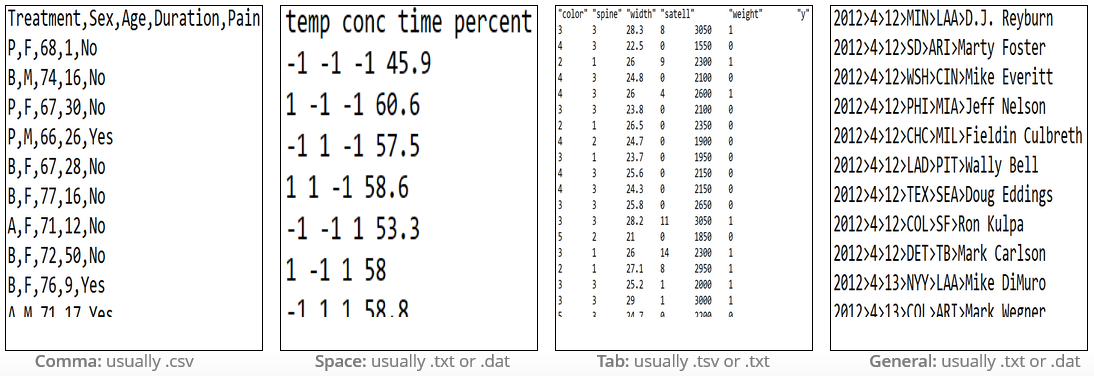
\includegraphics[width=0.8\linewidth]{img/delimitedData} \end{center}

To read in data we'll need functions to do so. When you open R a few \texttt{packages} are loaded.

\begin{center}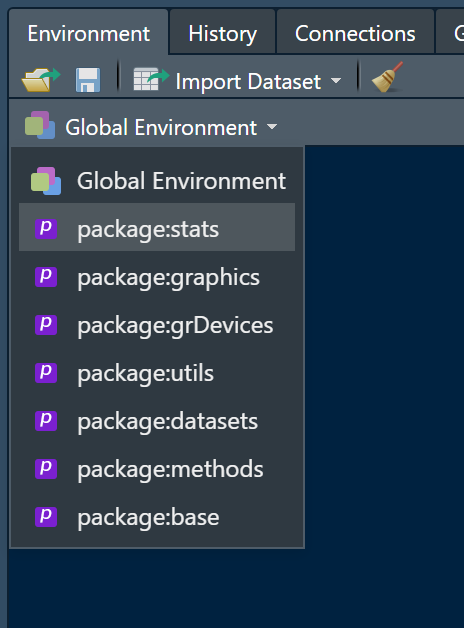
\includegraphics[width=0.2\linewidth]{img/loadR} \end{center}

R Packages:

\begin{itemize}
\item
  Collection of functions/datasets/etc. in one place
\item
  Packages exist to do almost anything
\item
  \href{https://cran.r-project.org/web/packages/available_packages_by_name.html}{List of CRAN} approved packages on R's website
\item
  Plenty of other packages on places like GitHub
\end{itemize}

The \texttt{utils} package that automatically loads has a \emph{family} of \texttt{read.} functions ready for use! Reading data with these functions is often referred to as reading with a standard R or base R method.

Function and purpose:

\begin{longtable}[]{@{}ll@{}}
\toprule
Type of Delimeter & Function\tabularnewline
\midrule
\endhead
Comma & \texttt{read.csv()}\tabularnewline
Semicolon (\texttt{,} for decimal) & \texttt{read.csv2()}\tabularnewline
Tab & \texttt{read.delim()}\tabularnewline
White Space/General & \texttt{read.table(sep\ =\ "")}\tabularnewline
\bottomrule
\end{longtable}

Each of these functions requires a \textbf{path} to the file in order to read it in. Let's read in the `\href{https://www4.stat.ncsu.edu/~online/datasets/neuralgia.csv}{neuralgia.csv}' file. This is a comma separated value file (.csv). This requires the \texttt{read.csv} function.

R locates the file by the path you give it. You can give \emph{full path name}. For example,

\begin{itemize}
\tightlist
\item
  ex: C:/Users/jbpost2/repos/StatisticalMethods/datasets/neuralgia.csv\\
\item
  ex: C:\textbackslash{}\textbackslash{}Users\textbackslash{}\textbackslash{}jbpost2\textbackslash{}\textbackslash{}repos\textbackslash{}\textbackslash{}StatisticalMethods\textbackslash{}\textbackslash{}datasets\textbackslash{}\textbackslash{}neuralgia.csv
\end{itemize}

\begin{center}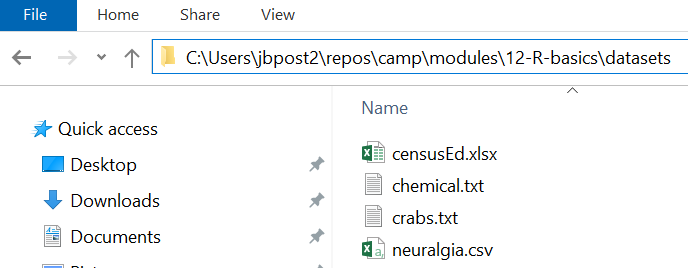
\includegraphics[width=0.8\linewidth]{img/pathVis} \end{center}

Notice that a double \texttt{\textbackslash{}} is needed because \texttt{\textbackslash{}} is an escape character in R so \texttt{\textbackslash{}\textbackslash{}} is really read as \texttt{\textbackslash{}}.

Ok, let's read in the neuralgia csv file using \texttt{read.csv}.

\begin{Shaded}
\begin{Highlighting}[]
\NormalTok{neuralgiaData <-}\StringTok{ }\KeywordTok{read.csv}\NormalTok{(}
           \StringTok{"C:/Users/jbpost2/repos/StatisticalMethods/datasets/neuralgia.csv"}
\NormalTok{           )}
\end{Highlighting}
\end{Shaded}

\begin{Shaded}
\begin{Highlighting}[]
\KeywordTok{head}\NormalTok{(neuralgiaData)}
\end{Highlighting}
\end{Shaded}

\begin{verbatim}
##   Treatment Sex Age Duration Pain
## 1         P   F  68        1   No
## 2         B   M  74       16   No
## 3         P   F  67       30   No
## 4         P   M  66       26  Yes
## 5         B   F  67       28   No
## 6         B   F  77       16   No
\end{verbatim}

Pretty simply if the data is nicely formatted! Using a full local path not recommended though! Doing so makes it difficult to share code without having to go in and change the paths. Instead, you can change the \emph{working directory} R is using. That is, the folder by default R is `looking' for files. Then we can supply a \textbf{relative} path. As long as other users have the same folder structure as you (say if you are using a github repo), no changes need to be made for them to run the code!

We can determine the working directory using \texttt{getwd}.

\begin{Shaded}
\begin{Highlighting}[]
\KeywordTok{getwd}\NormalTok{()}
\end{Highlighting}
\end{Shaded}

\begin{verbatim}
## [1] "C:/Users/jbpost2/repos/StatisticalMethods"
\end{verbatim}

This can be changed using \texttt{setwd}.

\begin{Shaded}
\begin{Highlighting}[]
\KeywordTok{setwd}\NormalTok{(}\StringTok{"C:/Users/jbpost2/repos/StatisticalMethods/datasets"}\NormalTok{)}
\CommentTok{#or}
\KeywordTok{setwd}\NormalTok{(}\StringTok{"C:}\CharTok{\textbackslash{}\textbackslash{}}\StringTok{Users}\CharTok{\textbackslash{}\textbackslash{}}\StringTok{jbpost2}\CharTok{\textbackslash{}\textbackslash{}}\StringTok{repos}\CharTok{\textbackslash{}\textbackslash{}}\StringTok{StatisticalMethods}\CharTok{\textbackslash{}\textbackslash{}}\StringTok{datasets"}\NormalTok{)}
\end{Highlighting}
\end{Shaded}

The working directory can also be changed via the menus in RStudio.

\begin{center}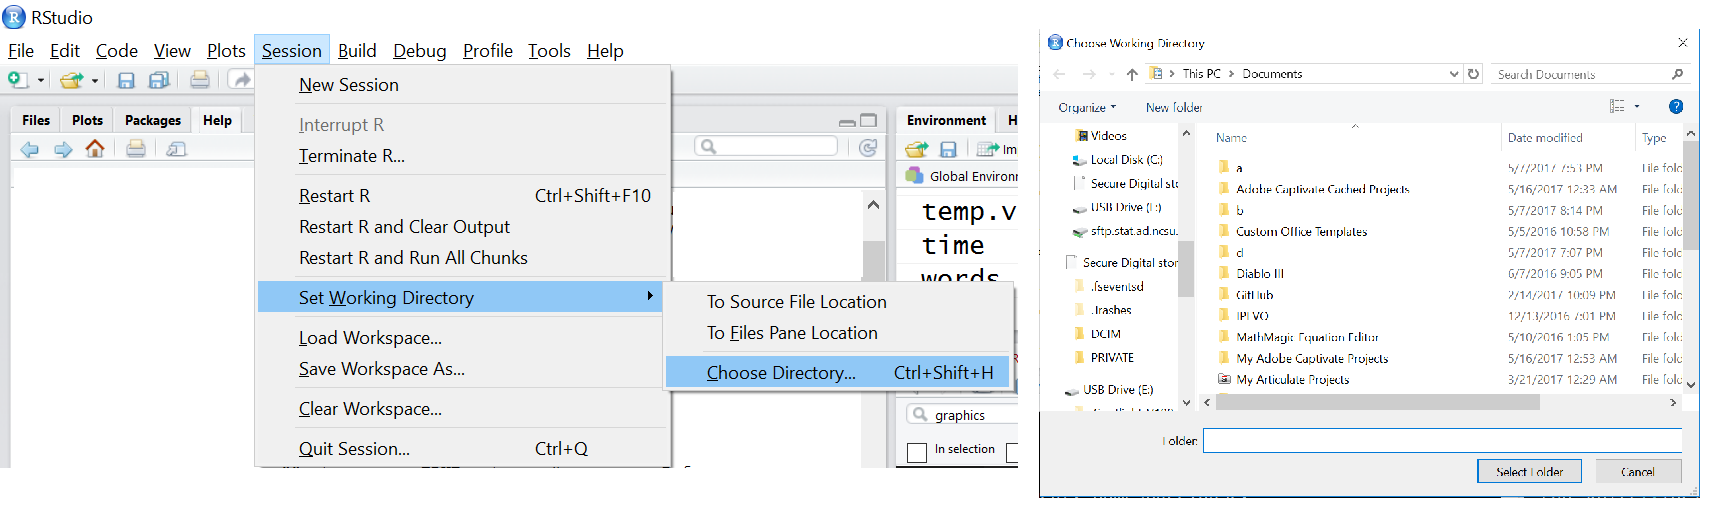
\includegraphics[width=0.8\linewidth]{img/setwd} \end{center}

Another way to supply a path is via a URL. This is really handy if you have a place to host your datasets!

\begin{Shaded}
\begin{Highlighting}[]
\NormalTok{neuralgiaData <-}\StringTok{ }\KeywordTok{read.csv}\NormalTok{(}\StringTok{"https://www4.stat.ncsu.edu/~online/datasets/neuralgia.csv"}\NormalTok{)}
\end{Highlighting}
\end{Shaded}

To recap, to read a csv file you can

\begin{itemize}
\item
  Use full local path (not recommended)
\item
  Use relative path

  \begin{itemize}
  \tightlist
  \item
    set working directory with \texttt{setwd()}
  \end{itemize}
\item
  Pull from a URL
\end{itemize}

\hypertarget{quick-aside-rstudio-project}{%
\subsection{Quick Aside: RStudio Project}\label{quick-aside-rstudio-project}}

Often we have many files associated with an analysis. When working on multiple undertakings things get cluttered in R\ldots{} With each analysis we may want to associate different

\begin{verbatim}
+ environments  
+ histories  
+ working directories  
+ source documents  
\end{verbatim}

The ``Project'' feature in R Studio allows us to easily do this! To create you can use the drop down menus.

\begin{center}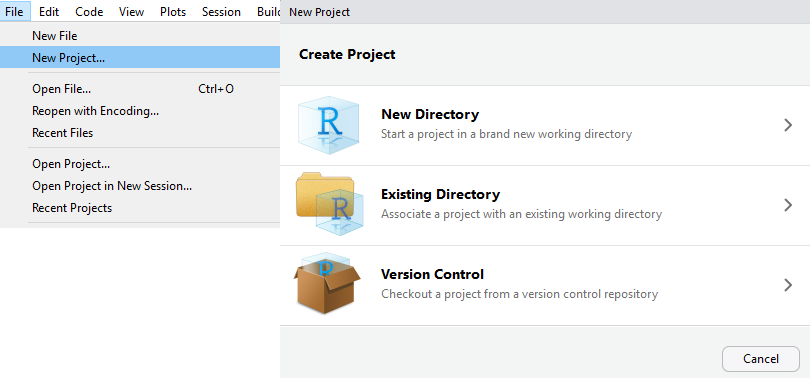
\includegraphics[width=0.8\linewidth]{img/project} \end{center}

Now you can easily switch between analyses by using ``File --\textgreater{} Open Project'' or by using the little drop down menu in the top right of RStudio.

\hypertarget{quick-aside-factors}{%
\subsection{Quick Aside: Factors}\label{quick-aside-factors}}

As mentioned above there are \texttt{read.} functions for many different types of delimited data. These functions work really well but there are a few areas they could be improved.

\begin{itemize}
\tightlist
\item
  A poor default function behavior as strings are read as \texttt{factors}
\end{itemize}

Understanding factors is important enough to warrant a quick discussion. Let's look at the structure of our neuralgiaData object we read in with \texttt{read.csv}.

\begin{Shaded}
\begin{Highlighting}[]
\KeywordTok{str}\NormalTok{(neuralgiaData)}
\end{Highlighting}
\end{Shaded}

\begin{verbatim}
## 'data.frame':    60 obs. of  5 variables:
##  $ Treatment: Factor w/ 3 levels "A","B","P": 3 2 3 3 2 2 1 2 2 1 ...
##  $ Sex      : Factor w/ 2 levels "F","M": 1 2 1 2 1 1 1 1 1 2 ...
##  $ Age      : int  68 74 67 66 67 77 71 72 76 71 ...
##  $ Duration : int  1 16 30 26 28 16 12 50 9 17 ...
##  $ Pain     : Factor w/ 2 levels "No","Yes": 1 1 1 2 1 1 1 1 2 2 ...
\end{verbatim}

We can see that all of the character variables are \texttt{Factor} vectors. A factor is a special class of vector with a \texttt{levels} attribute. The levels define all possible values for that variable. This is a great concept for a variable that can only take on certain values such as \texttt{Day} (Monday, Tuesday, \ldots{}, Sunday). However, if you have a variable like \texttt{Name} that you will eventually add new values (levels) to factors become a bit of a nuisance.

For example, in the neuralgia dataset we may have a fourth treatment we want to add to the \texttt{Treatment} variable. Let's try to assign the first observation value with a `new' treatment called `M'.

\begin{Shaded}
\begin{Highlighting}[]
\NormalTok{neuralgiaData}\OperatorTok{$}\NormalTok{Treatment}
\end{Highlighting}
\end{Shaded}

\begin{verbatim}
##  [1] P B P P B B A B B A A A B A P A P A P B B A A A B P B B P P A A B B B A P B
## [39] B P P P A B A P P A B P P P B A P A P A B A
## Levels: A B P
\end{verbatim}

\begin{Shaded}
\begin{Highlighting}[]
\NormalTok{neuralgiaData}\OperatorTok{$}\NormalTok{Treatment[}\DecValTok{1}\NormalTok{] <-}\StringTok{ "M"}
\end{Highlighting}
\end{Shaded}

\begin{verbatim}
## Warning in `[<-.factor`(`*tmp*`, 1, value = structure(c(NA, 2L, 3L, 3L, :
## invalid factor level, NA generated
\end{verbatim}

We can see this throws an error because `M' is not one of the levels defined for the variable. To add the new value we have to alter the \texttt{levels} attribute of the factor.

\begin{Shaded}
\begin{Highlighting}[]
\CommentTok{#overwrite with another possible level}
\KeywordTok{levels}\NormalTok{(neuralgiaData}\OperatorTok{$}\NormalTok{Treatment) <-}\StringTok{ }\KeywordTok{c}\NormalTok{(}\KeywordTok{levels}\NormalTok{(neuralgiaData}\OperatorTok{$}\NormalTok{Treatment), }\StringTok{"M"}\NormalTok{)}
\KeywordTok{levels}\NormalTok{(neuralgiaData}\OperatorTok{$}\NormalTok{Treatment)}
\end{Highlighting}
\end{Shaded}

\begin{verbatim}
## [1] "A" "B" "P" "M"
\end{verbatim}

\begin{Shaded}
\begin{Highlighting}[]
\NormalTok{neuralgiaData}\OperatorTok{$}\NormalTok{Treatment[}\DecValTok{1}\NormalTok{] <-}\StringTok{ "M"}
\end{Highlighting}
\end{Shaded}

Factors are very useful for plotting as we'll see later.

For the other issues with the \texttt{read.} family we can look at useful functions from other R packages. R packages deserve a brief discussion as well!

\hypertarget{quick-aside-r-packages}{%
\subsection{Quick Aside: R Packages}\label{quick-aside-r-packages}}

An R package is a collection of functions in one place. There are tons of packages to do most anything. In particular a group of packages called the ``\href{http://tidyverse.org/}{TidyVerse}'' has modernized the use of R for a larger audience. The tidyverse is a package that is a collection of eight R packages that share common philosophies and are designed to work together! One of these packages, \texttt{readr}, is extremely useful for reading in data and remedies the concerns mentioned above about the \texttt{read.} family of functions.

The first time using a package you must `install' the package (download the files). You can do this

\begin{itemize}
\tightlist
\item
  Using code:
\end{itemize}

\begin{Shaded}
\begin{Highlighting}[]
\KeywordTok{install.packages}\NormalTok{(}\StringTok{"tidyverse"}\NormalTok{)}
\CommentTok{#can do multiple packages at once}
\KeywordTok{install.packages}\NormalTok{(}\KeywordTok{c}\NormalTok{(}\StringTok{"readr"}\NormalTok{, }\StringTok{"readxl"}\NormalTok{, }\StringTok{"haven"}\NormalTok{, }\StringTok{"DBI"}\NormalTok{, }\StringTok{"httr"}\NormalTok{))}
\end{Highlighting}
\end{Shaded}

\begin{itemize}
\tightlist
\item
  Using menus:
\end{itemize}

\begin{center}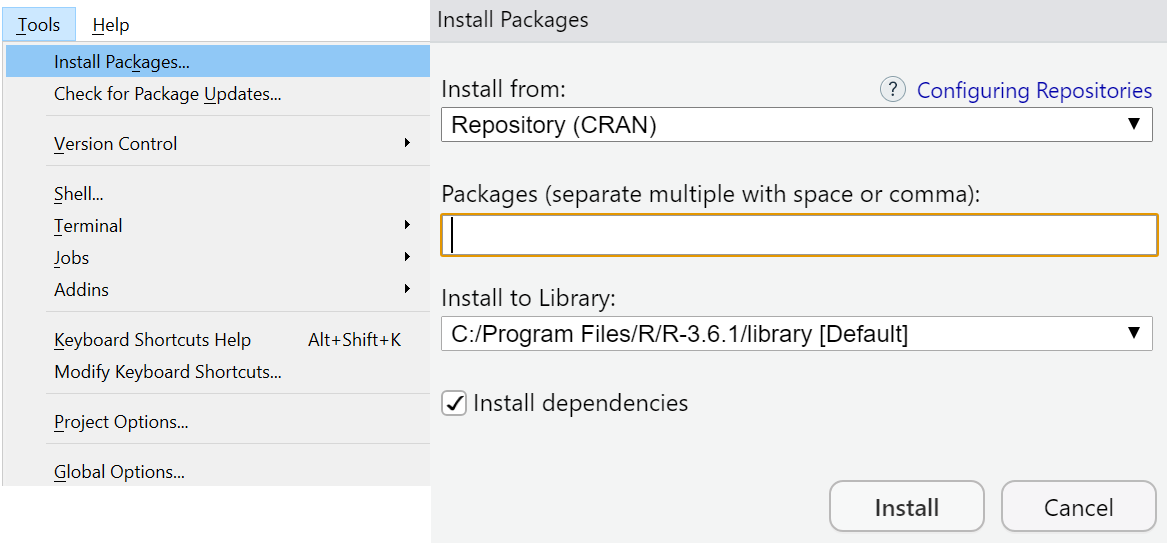
\includegraphics[width=0.7\linewidth]{img/packages} \end{center}

Note that you can also install packages from local sources (such as a downloaded .zip or .tar) but that isn't usually required unless you are behind a firewall or R updates and the packages haven't bene updated for that version of R.

The good thing is that you only need to install the packages once! However, this doesn't mean you have direct access to your package functions or datasets in your R session. \textbf{Each R session} you open you need to read in the package using \texttt{library()} or \texttt{require()}.

\begin{Shaded}
\begin{Highlighting}[]
\KeywordTok{library}\NormalTok{(}\StringTok{"readr"}\NormalTok{)}
\end{Highlighting}
\end{Shaded}

\begin{verbatim}
## Warning: package 'readr' was built under R version 3.6.2
\end{verbatim}

\begin{Shaded}
\begin{Highlighting}[]
\KeywordTok{require}\NormalTok{(}\StringTok{"haven"}\NormalTok{)}
\end{Highlighting}
\end{Shaded}

\begin{verbatim}
## Loading required package: haven
\end{verbatim}

\begin{verbatim}
## Warning: package 'haven' was built under R version 3.6.2
\end{verbatim}

These functions are very similar; they both give you direct access to the functions or data in your R session. The difference is that if you try to load a package that doesn't exist \texttt{library} throws an error where \texttt{require()} returns \texttt{FALSE}.

\begin{Shaded}
\begin{Highlighting}[]
\KeywordTok{library}\NormalTok{(}\StringTok{"notAPackage"}\NormalTok{)}
\end{Highlighting}
\end{Shaded}

\begin{verbatim}
## Error in library("notAPackage"): there is no package called 'notAPackage'
\end{verbatim}

\begin{Shaded}
\begin{Highlighting}[]
\KeywordTok{require}\NormalTok{(}\StringTok{"notAPackage"}\NormalTok{)}
\end{Highlighting}
\end{Shaded}

\begin{verbatim}
## Loading required package: notAPackage
\end{verbatim}

\begin{verbatim}
## Warning in library(package, lib.loc = lib.loc, character.only = TRUE,
## logical.return = TRUE, : there is no package called 'notAPackage'
\end{verbatim}

Now is a good time to install the \texttt{tidyverse} package if you haven't already.

\begin{Shaded}
\begin{Highlighting}[]
\KeywordTok{install.packages}\NormalTok{(}\StringTok{"tidyverse"}\NormalTok{)}
\end{Highlighting}
\end{Shaded}

The functions in the \texttt{tidyverse} generally have

\begin{itemize}
\item
  Fast code
\item
  Easy syntax
\item
  Good default settings on functions
\item
  A nice set of examples and vignettes
\end{itemize}

Read the package into your R session.

\begin{Shaded}
\begin{Highlighting}[]
\KeywordTok{library}\NormalTok{(tidyverse)}
\end{Highlighting}
\end{Shaded}

\begin{verbatim}
## Warning: package 'tidyverse' was built under R version 3.6.2
\end{verbatim}

\begin{verbatim}
## -- Attaching packages ----------------------------------------------------- tidyverse 1.3.0 --
\end{verbatim}

\begin{verbatim}
## v ggplot2 3.2.1     v dplyr   0.8.3
## v tibble  2.1.3     v stringr 1.4.0
## v tidyr   1.0.0     v forcats 0.4.0
## v purrr   0.3.3
\end{verbatim}

\begin{verbatim}
## Warning: package 'ggplot2' was built under R version 3.6.2
\end{verbatim}

\begin{verbatim}
## Warning: package 'tibble' was built under R version 3.6.2
\end{verbatim}

\begin{verbatim}
## Warning: package 'tidyr' was built under R version 3.6.2
\end{verbatim}

\begin{verbatim}
## Warning: package 'purrr' was built under R version 3.6.2
\end{verbatim}

\begin{verbatim}
## Warning: package 'dplyr' was built under R version 3.6.2
\end{verbatim}

\begin{verbatim}
## Warning: package 'stringr' was built under R version 3.6.2
\end{verbatim}

\begin{verbatim}
## Warning: package 'forcats' was built under R version 3.6.2
\end{verbatim}

\begin{verbatim}
## -- Conflicts -------------------------------------------------------- tidyverse_conflicts() --
## x dplyr::filter() masks stats::filter()
## x dplyr::lag()    masks stats::lag()
\end{verbatim}

You'll likely see a message about functions being masked. This implies that one of the functions just loaded has a function under the same name as a function that already exists. If you type \texttt{help(filter)}, R will now give you an option of which \texttt{filter} to look at. R uses the most recently loaded function and ``masks'' the old ones. You can access specific package's functions using \texttt{::}. This allows you to call functions without loading a full library.

\begin{Shaded}
\begin{Highlighting}[]
\NormalTok{readr}\OperatorTok{::}\KeywordTok{read_csv}\NormalTok{(}\StringTok{"https://www4.stat.ncsu.edu/~online/datasets/neuralgia.csv"}\NormalTok{)}
\end{Highlighting}
\end{Shaded}

\begin{verbatim}
## Parsed with column specification:
## cols(
##   Treatment = col_character(),
##   Sex = col_character(),
##   Age = col_double(),
##   Duration = col_double(),
##   Pain = col_character()
## )
\end{verbatim}

\begin{verbatim}
## # A tibble: 60 x 5
##   Treatment Sex     Age Duration Pain 
##   <chr>     <chr> <dbl>    <dbl> <chr>
## 1 P         F        68        1 No   
## 2 B         M        74       16 No   
## 3 P         F        67       30 No   
## 4 P         M        66       26 Yes  
## 5 B         F        67       28 No   
## # ... with 55 more rows
\end{verbatim}

\hypertarget{reading-delimited-data}{%
\subsection{Reading Delimited Data}\label{reading-delimited-data}}

Again the \texttt{read.} functions exist to read in many different types of delimited data. These functions work really well but there are a few areas they could be improved.

\begin{itemize}
\item
  A poor default function behavior as strings are read as \texttt{factors}
\item
  Raw data row \& column names can be troublesome
\item
  Slow processing (relatively speaking)
\item
  (Slightly) different behavior on different computers
\end{itemize}

Functions from the \texttt{tidyverse} (and \texttt{readr} in particular) remedy all of these!

\begin{longtable}[]{@{}lll@{}}
\toprule
Type of Delimeter & \texttt{utils} Function & \texttt{readr}\tabularnewline
\midrule
\endhead
Comma & \texttt{read.csv()} & \texttt{read\_csv()}\tabularnewline
Semicolon (\texttt{,} for decimal) & \texttt{read.csv2()} & \texttt{read\_csv2()}\tabularnewline
Tab & \texttt{read.delim()} & \texttt{read\_tsv()}\tabularnewline
General & \texttt{read.table(sep\ =\ "")} & \texttt{read\_delim()}\tabularnewline
White Space & \texttt{read.table(sep\ =\ "")} & \texttt{read\_table()} \texttt{read\_table2()}\tabularnewline
\bottomrule
\end{longtable}

Let's reread the `\href{https://www4.stat.ncsu.edu/~online/datasets/neuralgia.csv}{neuralgia.csv}' file using \texttt{read\_csv} from the \texttt{readr} package.

\begin{Shaded}
\begin{Highlighting}[]
\NormalTok{neuralgiaData <-}\StringTok{ }\NormalTok{readr}\OperatorTok{::}\KeywordTok{read_csv}\NormalTok{(}\StringTok{"https://www4.stat.ncsu.edu/~online/datasets/neuralgia.csv"}\NormalTok{)}
\end{Highlighting}
\end{Shaded}

\begin{verbatim}
## Parsed with column specification:
## cols(
##   Treatment = col_character(),
##   Sex = col_character(),
##   Age = col_double(),
##   Duration = col_double(),
##   Pain = col_character()
## )
\end{verbatim}

You can see that the package displays a bit of information about how the data was parsed.

\begin{Shaded}
\begin{Highlighting}[]
\NormalTok{neuralgiaData}
\end{Highlighting}
\end{Shaded}

\begin{verbatim}
## # A tibble: 60 x 5
##   Treatment Sex     Age Duration Pain 
##   <chr>     <chr> <dbl>    <dbl> <chr>
## 1 P         F        68        1 No   
## 2 B         M        74       16 No   
## 3 P         F        67       30 No   
## 4 P         M        66       26 Yes  
## 5 B         F        67       28 No   
## # ... with 55 more rows
\end{verbatim}

You'll also notice the fancy printing. This gives a quick check for the column type you have, which is a basic data validation step. The \texttt{tidyverse} has a special class of data frames called \texttt{tibbles}.

\begin{Shaded}
\begin{Highlighting}[]
\KeywordTok{class}\NormalTok{(neuralgiaData)}
\end{Highlighting}
\end{Shaded}

\begin{verbatim}
## [1] "spec_tbl_df" "tbl_df"      "tbl"         "data.frame"
\end{verbatim}

The behavior of \texttt{tibbles} is slightly different than that of a standard \texttt{data\ frame}. One is the printing method. The other major difference is that \texttt{tibbles} don't simplify.

\begin{Shaded}
\begin{Highlighting}[]
\NormalTok{neuralgiaData[,}\DecValTok{1}\NormalTok{]}
\end{Highlighting}
\end{Shaded}

\begin{verbatim}
## # A tibble: 60 x 1
##   Treatment
##   <chr>    
## 1 P        
## 2 B        
## 3 P        
## 4 P        
## 5 B        
## # ... with 55 more rows
\end{verbatim}

\begin{Shaded}
\begin{Highlighting}[]
\KeywordTok{as.data.frame}\NormalTok{(neuralgiaData)[,}\DecValTok{1}\NormalTok{]}
\end{Highlighting}
\end{Shaded}

\begin{verbatim}
##  [1] "P" "B" "P" "P" "B" "B" "A" "B" "B" "A" "A" "A" "B" "A" "P" "A" "P" "A" "P"
## [20] "B" "B" "A" "A" "A" "B" "P" "B" "B" "P" "P" "A" "A" "B" "B" "B" "A" "P" "B"
## [39] "B" "P" "P" "P" "A" "B" "A" "P" "P" "A" "B" "P" "P" "P" "B" "A" "P" "A" "P"
## [58] "A" "B" "A"
\end{verbatim}

As this behavior can cause some issues with functions that are expecting a vector it is useful to force simplification sometimes. You can either use the \texttt{pull} function or the \texttt{\$} operator to return a column as a vector.

\begin{Shaded}
\begin{Highlighting}[]
\KeywordTok{pull}\NormalTok{(neuralgiaData, }\DecValTok{1}\NormalTok{)}
\end{Highlighting}
\end{Shaded}

\begin{verbatim}
##  [1] "P" "B" "P" "P" "B" "B" "A" "B" "B" "A" "A" "A" "B" "A" "P" "A" "P" "A" "P"
## [20] "B" "B" "A" "A" "A" "B" "P" "B" "B" "P" "P" "A" "A" "B" "B" "B" "A" "P" "B"
## [39] "B" "P" "P" "P" "A" "B" "A" "P" "P" "A" "B" "P" "P" "P" "B" "A" "P" "A" "P"
## [58] "A" "B" "A"
\end{verbatim}

\begin{Shaded}
\begin{Highlighting}[]
\NormalTok{neuralgiaData}\OperatorTok{$}\NormalTok{Treatment }
\end{Highlighting}
\end{Shaded}

\begin{verbatim}
##  [1] "P" "B" "P" "P" "B" "B" "A" "B" "B" "A" "A" "A" "B" "A" "P" "A" "P" "A" "P"
## [20] "B" "B" "A" "A" "A" "B" "P" "B" "B" "P" "P" "A" "A" "B" "B" "B" "A" "P" "B"
## [39] "B" "P" "P" "P" "A" "B" "A" "P" "P" "A" "B" "P" "P" "P" "B" "A" "P" "A" "P"
## [58] "A" "B" "A"
\end{verbatim}

One question you may have about the column types is, how did R determine the column types? The help file for \texttt{read\_csv} tells us that it checks the first 1000 rows of data and uses those to figure out the type of data. You can of course override this default behavior.

Some useful inputs you may want to change when reading in data are

\begin{itemize}
\item
  \texttt{skip\ =\ 0}
\item
  \texttt{col\_names\ =\ TRUE}
\item
  \texttt{na\ =\ c("",\ "NA")}
\end{itemize}

These allow you to skip lines of data, specify column names, and define what represents a missing value in the raw data (\texttt{NA} is the missing data indicator in R).

Generally, reading \emph{clean} delimited data pretty easy with the \texttt{read\_} family of functions! Let's go through a few examples.

First, let's read in the space delimited file `\href{https://www4.stat.ncsu.edu/~online/datasets/chemical.txt}{chemical.txt}'. Since this is space delimited we'll use \texttt{read\_table}.

\begin{Shaded}
\begin{Highlighting}[]
\KeywordTok{read_table}\NormalTok{(}\StringTok{"https://www4.stat.ncsu.edu/~online/datasets/chemical.txt"}\NormalTok{)}
\end{Highlighting}
\end{Shaded}

\begin{verbatim}
## Parsed with column specification:
## cols(
##   `temp conc time percent` = col_character()
## )
\end{verbatim}

\begin{verbatim}
## # A tibble: 19 x 1
##    `temp conc time percent`
##    <chr>                   
##  1 -1 -1 -1 45.9           
##  2 1 -1 -1 60.6            
##  3 -1 1 -1 57.5            
##  4 1 1 -1 58.6             
##  5 -1 -1 1 53.3            
##  6 1 -1 1 58               
##  7 -1 1 1 58.8             
##  8 1 1 1 52.4              
##  9 -2 0 0 46.9             
## 10 2 0 0 55.4              
## 11 0 -2 0 55               
## 12 0 2 0 57.5              
## 13 0 0 -2 56.3             
## 14 0 0 2 58.9              
## 15 0 0 0 56.9              
## 16 2 -3 0 61.1             
## 17 2 -3 0 62.9             
## 18 -1.4 2.6 0.7 60         
## 19 -1.4 2.6 0.7 60.6
\end{verbatim}

Next, let's read in the tab delimited file `\href{https://www4.stat.ncsu.edu/~online/datasets/crabs.txt}{crabs.txt}'. Since this is tab delimited we'll use \texttt{read\_tsv}.

\begin{Shaded}
\begin{Highlighting}[]
\KeywordTok{read_tsv}\NormalTok{(}\StringTok{"https://www4.stat.ncsu.edu/~online/datasets/crabs.txt"}\NormalTok{)}
\end{Highlighting}
\end{Shaded}

\begin{verbatim}
## Parsed with column specification:
## cols(
##   color = col_double(),
##   spine = col_double(),
##   width = col_double(),
##   satell = col_double(),
##   weight = col_double(),
##   y = col_double()
## )
\end{verbatim}

\begin{verbatim}
## # A tibble: 173 x 6
##   color spine width satell weight     y
##   <dbl> <dbl> <dbl>  <dbl>  <dbl> <dbl>
## 1     3     3  28.3      8   3050     1
## 2     4     3  22.5      0   1550     0
## 3     2     1  26        9   2300     1
## 4     4     3  24.8      0   2100     0
## 5     4     3  26        4   2600     1
## # ... with 168 more rows
\end{verbatim}

Lastly, let's read in the \texttt{\textgreater{}} delimited file `\href{https://www4.stat.ncsu.edu/~online/datasets/umps2012.txt}{umps2012.txt}'. As this isn't a standard delimiter we'll use \texttt{read\_delim} and specify the \texttt{delim\ =} input. However, this file doesn't contain column names in the raw data. The columns represent Year, Month, Day, Home, Away, and HPUmpire. The column names can be specified using the \texttt{col\_names} input and specifying them with a character vector.

\begin{Shaded}
\begin{Highlighting}[]
\KeywordTok{read_delim}\NormalTok{(}\StringTok{"https://www4.stat.ncsu.edu/~online/datasets/umps2012.txt"}\NormalTok{, }\DataTypeTok{delim =} \StringTok{">"}\NormalTok{,}
           \DataTypeTok{col_names =} \KeywordTok{c}\NormalTok{(}\StringTok{"Year"}\NormalTok{, }\StringTok{"Month"}\NormalTok{, }\StringTok{"Day"}\NormalTok{, }\StringTok{"Home"}\NormalTok{, }\StringTok{"Away"}\NormalTok{, }\StringTok{"HPUmpire"}\NormalTok{))}
\end{Highlighting}
\end{Shaded}

\begin{verbatim}
## Parsed with column specification:
## cols(
##   Year = col_double(),
##   Month = col_double(),
##   Day = col_double(),
##   Home = col_character(),
##   Away = col_character(),
##   HPUmpire = col_character()
## )
\end{verbatim}

\begin{verbatim}
## # A tibble: 2,359 x 6
##    Year Month   Day Home  Away  HPUmpire        
##   <dbl> <dbl> <dbl> <chr> <chr> <chr>           
## 1  2012     4    12 MIN   LAA   D.J. Reyburn    
## 2  2012     4    12 SD    ARI   Marty Foster    
## 3  2012     4    12 WSH   CIN   Mike Everitt    
## 4  2012     4    12 PHI   MIA   Jeff Nelson     
## 5  2012     4    12 CHC   MIL   Fieldin Culbreth
## # ... with 2,354 more rows
\end{verbatim}

\hypertarget{non-standard-data}{%
\subsubsection{Non-Standard Data}\label{non-standard-data}}

To read in tricky, non-standard data there are a few functions that can help.

\begin{itemize}
\item
  \texttt{read\_file} - reads an entire file into a single string
\item
  \texttt{read\_lines} - reads a file into a character vector with one element per line
\end{itemize}

These are often parsed with \texttt{regular\ expressions}.

\hypertarget{excel-data}{%
\subsection{Excel data}\label{excel-data}}

Next we'll cover reading data from Excel files (\texttt{readxl} package), SAS datasets (\texttt{haven} package), and SPSS files (\texttt{haven} package).

\begin{longtable}[]{@{}lll@{}}
\toprule
Type of file & Package & Function\tabularnewline
\midrule
\endhead
Delimited & \texttt{readr} & \texttt{read\_csv()}, \texttt{read\_tsv()},\texttt{read\_table()}, \texttt{read\_delim()}\tabularnewline
Excel (.xls,.xlsx) & \texttt{readxl} & \texttt{read\_excel()}\tabularnewline
SAS (.sas7bdat) & \texttt{haven} & \texttt{read\_sas()}\tabularnewline
SPSS (.sav) & \texttt{haven} & \texttt{read\_spss()}\tabularnewline
\bottomrule
\end{longtable}

Let's read in the \href{https://www4.stat.ncsu.edu/~online/datasets/censusEd.xlsx}{censusEd.xlsx} file.This can be done with the \texttt{read\_excel()} from \texttt{readxl} package! This funcion reads in both xls and xlsx files. It detects the format from the file extension given in the path name. One issue is that excel files can be read from the web so they do need to be downloaded locally.

\begin{Shaded}
\begin{Highlighting}[]
\CommentTok{#install package if necessary}
\KeywordTok{library}\NormalTok{(readxl)}
\end{Highlighting}
\end{Shaded}

\begin{verbatim}
## Warning: package 'readxl' was built under R version 3.6.2
\end{verbatim}

\begin{Shaded}
\begin{Highlighting}[]
\CommentTok{#reads first sheet by default}
\NormalTok{edData <-}\StringTok{ }\KeywordTok{read_excel}\NormalTok{(}\StringTok{"datasets/censusEd.xlsx"}\NormalTok{)}
\NormalTok{edData}
\end{Highlighting}
\end{Shaded}

\begin{verbatim}
## # A tibble: 3,198 x 42
##   Area_name STCOU EDU010187F EDU010187D EDU010187N1 EDU010187N2 EDU010188F
##   <chr>     <chr>      <dbl>      <dbl> <chr>       <chr>            <dbl>
## 1 UNITED S~ 00000          0   40024299 0000        0000                 0
## 2 ALABAMA   01000          0     733735 0000        0000                 0
## 3 Autauga,~ 01001          0       6829 0000        0000                 0
## 4 Baldwin,~ 01003          0      16417 0000        0000                 0
## 5 Barbour,~ 01005          0       5071 0000        0000                 0
## # ... with 3,193 more rows, and 35 more variables: EDU010188D <dbl>,
## #   EDU010188N1 <chr>, EDU010188N2 <chr>, EDU010189F <dbl>, EDU010189D <dbl>,
## #   EDU010189N1 <chr>, EDU010189N2 <chr>, EDU010190F <dbl>, EDU010190D <dbl>,
## #   EDU010190N1 <chr>, EDU010190N2 <chr>, EDU010191F <dbl>, EDU010191D <dbl>,
## #   EDU010191N1 <chr>, EDU010191N2 <chr>, EDU010192F <dbl>, EDU010192D <dbl>,
## #   EDU010192N1 <chr>, EDU010192N2 <chr>, EDU010193F <dbl>, EDU010193D <dbl>,
## #   EDU010193N1 <chr>, EDU010193N2 <chr>, EDU010194F <dbl>, EDU010194D <dbl>,
## #   EDU010194N1 <chr>, EDU010194N2 <chr>, EDU010195F <dbl>, EDU010195D <dbl>,
## #   EDU010195N1 <chr>, EDU010195N2 <chr>, EDU010196F <dbl>, EDU010196D <dbl>,
## #   EDU010196N1 <chr>, EDU010196N2 <chr>
\end{verbatim}

If you want to read in a sheet other than the first sheet, you can do so with the \texttt{sheet\ =} argument. To look at the available sheets without opening in Excel you can use the \texttt{excel\_sheets} function.

\begin{Shaded}
\begin{Highlighting}[]
\KeywordTok{excel_sheets}\NormalTok{(}\StringTok{"datasets/censusEd.xlsx"}\NormalTok{)}
\end{Highlighting}
\end{Shaded}

\begin{verbatim}
##  [1] "EDU01A" "EDU01B" "EDU01C" "EDU01D" "EDU01E" "EDU01F" "EDU01G" "EDU01H"
##  [9] "EDU01I" "EDU01J"
\end{verbatim}

\begin{Shaded}
\begin{Highlighting}[]
\KeywordTok{read_excel}\NormalTok{(}\StringTok{"datasets/censusEd.xlsx"}\NormalTok{, }\DataTypeTok{sheet =} \StringTok{"EDU01D"}\NormalTok{)}
\end{Highlighting}
\end{Shaded}

There are also ways to specify which cells to read in with the \texttt{range\ =} argument. You can select cells that are contiguous only (next to each other).

\begin{Shaded}
\begin{Highlighting}[]
\NormalTok{edData <-}\StringTok{ }\KeywordTok{read_excel}\NormalTok{(}\StringTok{"datasets/censusEd.xlsx"}\NormalTok{, }\DataTypeTok{sheet =} \StringTok{"EDU01A"}\NormalTok{, }
                   \DataTypeTok{range =} \KeywordTok{cell_cols}\NormalTok{(}\StringTok{"A:D"}\NormalTok{))}
\NormalTok{edData}
\end{Highlighting}
\end{Shaded}

\begin{verbatim}
## # A tibble: 3,198 x 4
##   Area_name     STCOU EDU010187F EDU010187D
##   <chr>         <chr>      <dbl>      <dbl>
## 1 UNITED STATES 00000          0   40024299
## 2 ALABAMA       01000          0     733735
## 3 Autauga, AL   01001          0       6829
## 4 Baldwin, AL   01003          0      16417
## 5 Barbour, AL   01005          0       5071
## # ... with 3,193 more rows
\end{verbatim}

\hypertarget{sas-data}{%
\subsection{SAS Data}\label{sas-data}}

SAS datasets have a file extension of `.sas7bdat'. Let's read in the \href{https://www4.stat.ncsu.edu/~online/datasets/smoke2003.sas7bdat}{smoke2003.sas7bdat} dataset. This can be done using the \texttt{read\_sas} function from the \texttt{haven} package. As .sas7bdat files are pretty structured there aren't many options to use with this function.

\begin{Shaded}
\begin{Highlighting}[]
\CommentTok{#install if necessary}
\KeywordTok{library}\NormalTok{(haven)}
\NormalTok{smokeData <-}\StringTok{ }\KeywordTok{read_sas}\NormalTok{(}\StringTok{"https://www4.stat.ncsu.edu/~online/datasets/smoke2003.sas7bdat"}\NormalTok{)}
\NormalTok{smokeData}
\end{Highlighting}
\end{Shaded}

\begin{verbatim}
## # A tibble: 443 x 54
##    SEQN SDDSRVYR RIDSTATR RIDEXMON RIAGENDR RIDAGEYR RIDAGEMN RIDAGEEX RIDRETH1
##   <dbl>    <dbl>    <dbl>    <dbl>    <dbl>    <dbl>    <dbl>    <dbl>    <dbl>
## 1 21010        3        2        2        2       52      633      634        3
## 2 21012        3        2        2        1       63      765      766        4
## 3 21048        3        2        1        2       42      504      504        1
## 4 21084        3        2        1        2       57      692      693        3
## 5 21093        3        2        1        2       64      778      778        2
## # ... with 438 more rows, and 45 more variables: RIDRETH2 <dbl>,
## #   DMQMILIT <dbl>, DMDBORN <dbl>, DMDCITZN <dbl>, DMDYRSUS <dbl>,
## #   DMDEDUC3 <dbl>, DMDEDUC2 <dbl>, DMDEDUC <dbl>, DMDSCHOL <dbl>,
## #   DMDMARTL <dbl>, DMDHHSIZ <dbl>, INDHHINC <dbl>, INDFMINC <dbl>,
## #   INDFMPIR <dbl>, RIDEXPRG <dbl>, DMDHRGND <dbl>, DMDHRAGE <dbl>,
## #   DMDHRBRN <dbl>, DMDHREDU <dbl>, DMDHRMAR <dbl>, DMDHSEDU <dbl>,
## #   SIALANG <dbl>, SIAPROXY <dbl>, SIAINTRP <dbl>, FIALANG <dbl>,
## #   FIAPROXY <dbl>, FIAINTRP <dbl>, MIALANG <dbl>, MIAPROXY <dbl>,
## #   MIAINTRP <dbl>, AIALANG <dbl>, WTINT2YR <dbl>, WTMEC2YR <dbl>,
## #   SDMVPSU <dbl>, SDMVSTRA <dbl>, Gender <dbl>, Age <dbl>, IncomeGroup <chr>,
## #   Ethnicity <chr>, Education <dbl>, SMD070 <dbl>, SMQ077 <dbl>, SMD650 <dbl>,
## #   PacksPerDay <dbl>, lbdvid <dbl>
\end{verbatim}

Often times SAS datasets have labels associated with the variable names. These are more descriptive titles that will print in SAS if requested. This is the case here. However, as you see above the labels did not print out. The labels will show if you look at the data set using the \texttt{View} function (or click on smokeData object from environment tab). How do we get to those labels?

\begin{Shaded}
\begin{Highlighting}[]
\KeywordTok{str}\NormalTok{(smokeData)}
\end{Highlighting}
\end{Shaded}

\begin{verbatim}
## Classes 'tbl_df', 'tbl' and 'data.frame':    443 obs. of  54 variables:
##  $ SEQN       : num  21010 21012 21048 21084 21093 ...
##   ..- attr(*, "label")= chr "Patient ID"
##  $ SDDSRVYR   : num  3 3 3 3 3 3 3 3 3 3 ...
##   ..- attr(*, "label")= chr "Data Release Number"
##  $ RIDSTATR   : num  2 2 2 2 2 2 2 2 2 2 ...
##   ..- attr(*, "label")= chr "Interview/Examination Status"
##  $ RIDEXMON   : num  2 2 1 1 1 2 1 2 1 1 ...
##   ..- attr(*, "label")= chr "Six month time period"
##  $ RIAGENDR   : num  2 1 2 2 2 2 1 2 1 2 ...
##   ..- attr(*, "label")= chr "Gender 1=M 2=F"
##  $ RIDAGEYR   : num  52 63 42 57 64 63 66 60 65 47 ...
##   ..- attr(*, "label")= chr "Age in Years at Exam"
##  $ RIDAGEMN   : num  633 765 504 692 778 763 801 731 786 573 ...
##   ..- attr(*, "label")= chr "Age in Months - Recode"
##  $ RIDAGEEX   : num  634 766 504 693 778 763 801 732 787 573 ...
##   ..- attr(*, "label")= chr "Exam Age in Months - Recode"
##  $ RIDRETH1   : num  3 4 1 3 2 3 1 3 3 3 ...
##   ..- attr(*, "label")= chr " Ethnicity 1=MexAm 2=OthHisp 3=OthCauc 4=OthBla 5=Oth"
##  $ RIDRETH2   : num  1 2 3 1 5 1 3 1 1 1 ...
##   ..- attr(*, "label")= chr "Linked NH3 Race/Ethnicity - Recode"
##  $ DMQMILIT   : num  2 2 2 2 2 2 2 2 1 2 ...
##   ..- attr(*, "label")= chr "Veteran/Military Status"
##  $ DMDBORN    : num  1 1 1 1 3 1 1 1 1 1 ...
##   ..- attr(*, "label")= chr "Country of Birth - Recode"
##  $ DMDCITZN   : num  1 1 1 1 1 1 1 1 1 1 ...
##   ..- attr(*, "label")= chr "Citizenship Status"
##  $ DMDYRSUS   : num  NA NA NA NA 9 NA NA NA NA NA ...
##   ..- attr(*, "label")= chr "Length of time in US"
##  $ DMDEDUC3   : num  NA NA NA NA NA NA NA NA NA NA ...
##   ..- attr(*, "label")= chr "Education Level - Children/Youth 6-19"
##  $ DMDEDUC2   : num  4 3 3 4 1 3 1 4 4 4 ...
##   ..- attr(*, "label")= chr "Education Level for Over 20"
##  $ DMDEDUC    : num  3 2 2 3 1 2 1 3 3 3 ...
##   ..- attr(*, "label")= chr "Education - Recode (old version)"
##  $ DMDSCHOL   : num  NA NA NA NA NA NA NA NA NA NA ...
##   ..- attr(*, "label")= chr "Now attending school?"
##  $ DMDMARTL   : num  6 6 3 1 2 1 6 3 1 1 ...
##   ..- attr(*, "label")= chr "Marital Status"
##  $ DMDHHSIZ   : num  3 2 5 2 2 2 2 3 2 6 ...
##   ..- attr(*, "label")= chr "Total number of people in the Household"
##  $ INDHHINC   : num  6 2 5 9 2 5 3 6 8 5 ...
##   ..- attr(*, "label")= chr "Annual Household Income"
##  $ INDFMINC   : num  4 2 2 9 2 5 3 6 8 4 ...
##   ..- attr(*, "label")= chr "Family Income"
##  $ INDFMPIR   : num  1.24 0.89 0.48 4.62 0.61 1.92 1.39 2.21 3.71 1.23 ...
##   ..- attr(*, "label")= chr "Family PIR"
##  $ RIDEXPRG   : num  2 NA 2 2 NA NA NA NA NA 2 ...
##   ..- attr(*, "label")= chr "Pregnancy Status at Exam - Recode"
##  $ DMDHRGND   : num  1 1 2 2 2 1 1 2 1 1 ...
##   ..- attr(*, "label")= chr "HH Ref Person Gender"
##  $ DMDHRAGE   : num  54 63 59 57 64 66 66 84 65 50 ...
##   ..- attr(*, "label")= chr "HH Ref Person Age"
##  $ DMDHRBRN   : num  1 1 1 1 3 1 1 1 1 NA ...
##   ..- attr(*, "label")= chr "HH Ref Person Country of Birth"
##  $ DMDHREDU   : num  1 3 4 4 1 3 1 5 4 NA ...
##   ..- attr(*, "label")= chr "HH Ref Person Education Level"
##  $ DMDHRMAR   : num  6 6 3 1 2 1 6 2 1 1 ...
##   ..- attr(*, "label")= chr "HH Ref Person Marital Status"
##  $ DMDHSEDU   : num  NA NA NA 3 NA 3 NA NA 2 4 ...
##   ..- attr(*, "label")= chr "HH Ref Person's Spouse Education Level"
##  $ SIALANG    : num  1 1 1 1 1 1 1 1 1 1 ...
##   ..- attr(*, "label")= chr "Language of SP Interview"
##  $ SIAPROXY   : num  2 2 2 2 2 2 2 2 2 2 ...
##   ..- attr(*, "label")= chr "Proxy used in SP Interview?"
##  $ SIAINTRP   : num  2 2 2 2 2 2 2 2 2 2 ...
##   ..- attr(*, "label")= chr "Interpreter used in SP Interview?"
##  $ FIALANG    : num  1 1 1 1 1 1 1 1 1 1 ...
##   ..- attr(*, "label")= chr "Language of Family Interview"
##  $ FIAPROXY   : num  2 2 2 2 2 2 2 2 2 2 ...
##   ..- attr(*, "label")= chr "Proxy used in Family Interview?"
##  $ FIAINTRP   : num  2 2 2 2 2 2 2 2 2 2 ...
##   ..- attr(*, "label")= chr "Interpreter used in Family Interview?"
##  $ MIALANG    : num  1 NA 1 1 1 1 1 1 1 1 ...
##   ..- attr(*, "label")= chr "Language of MEC Interview"
##  $ MIAPROXY   : num  2 NA 2 2 2 2 2 2 2 2 ...
##   ..- attr(*, "label")= chr "Proxy used in MEC Interview?"
##  $ MIAINTRP   : num  2 NA 2 2 2 2 2 2 2 2 ...
##   ..- attr(*, "label")= chr "Interpreter used in MEC Interview?"
##  $ AIALANG    : num  1 NA 1 1 NA NA NA NA NA 1 ...
##   ..- attr(*, "label")= chr "Language of ACASI Interview"
##  $ WTINT2YR   : num  39599 12629 18792 91437 24475 ...
##   ..- attr(*, "label")= chr "Full Sample 2 Year Interview Weight"
##  $ WTMEC2YR   : num  43287 12947 19035 93163 27829 ...
##   ..- attr(*, "label")= chr "Full Sample 2 Year MEC Exam Weight"
##  $ SDMVPSU    : num  1 2 2 1 1 2 1 2 1 2 ...
##   ..- attr(*, "label")= chr "Masked Variance Pseudo-PSU"
##  $ SDMVSTRA   : num  29 33 39 34 35 30 34 30 38 34 ...
##   ..- attr(*, "label")= chr "Masked Variance Pseudo-Stratum"
##  $ Gender     : num  2 1 2 2 2 2 1 2 1 2 ...
##  $ Age        : num  52 63 42 57 64 63 66 60 65 47 ...
##  $ IncomeGroup: chr  "Less Than 20K" "Less Than 20K" "Less Than 20K" "More Than 20K" ...
##  $ Ethnicity  : chr  "Non-Hispanic Caucasian" "Non-Hispanic Black" "MexicanAmerican & Hispanic" "Non-Hispanic Caucasian" ...
##  $ Education  : num  4 3 3 4 1 3 1 4 4 4 ...
##  $ SMD070     : num  20 20 20 20 20 16 20 20 10 6 ...
##   ..- attr(*, "label")= chr "Number of Cagarettes Smoked/day now"
##  $ SMQ077     : num  2 2 1 3 2 2 2 1 3 3 ...
##   ..- attr(*, "label")= chr "How soon after waking do you smoke?"
##  $ SMD650     : num  20 20 20 20 20 10 20 20 10 1 ...
##   ..- attr(*, "label")= chr "Number of Cigarettes/day for last 30 days"
##  $ PacksPerDay: num  1 1 1 1 1 0.5 1 1 0.5 0.05 ...
##  $ lbdvid     : num  16 18 16 17 18 25 9 27 9 25 ...
##  - attr(*, "label")= chr "DATA2003"
\end{verbatim}

The labels are an \textbf{attribute} of the dataset. The attribute is called ``label''. These can be accessed using the \texttt{attr} function.

\begin{Shaded}
\begin{Highlighting}[]
\KeywordTok{attr}\NormalTok{(smokeData}\OperatorTok{$}\NormalTok{SDDSRVYR, }\StringTok{"label"}\NormalTok{)}
\end{Highlighting}
\end{Shaded}

\begin{verbatim}
## [1] "Data Release Number"
\end{verbatim}

\hypertarget{spss-data}{%
\subsection{SPSS Data}\label{spss-data}}

SPSS datasets have a file extension of ``.sav''. Let's read in the \href{https://www4.stat.ncsu.edu/~online/datasets/bodyFat.sav}{bodyFat.sav} dataset. This can be done using the \texttt{read\_spss} function from the \texttt{haven} package. As with SAS datasets, these are well structured so there aren't many options to use with the function.

\begin{Shaded}
\begin{Highlighting}[]
\NormalTok{bodyFatData <-}\StringTok{ }\KeywordTok{read_spss}\NormalTok{(}\StringTok{"https://www4.stat.ncsu.edu/~online/datasets/bodyFat.sav"}\NormalTok{)}
\NormalTok{bodyFatData}
\end{Highlighting}
\end{Shaded}

\begin{verbatim}
## # A tibble: 20 x 4
##        y    x1    x2    x3
##    <dbl> <dbl> <dbl> <dbl>
##  1  19.5  43.1  29.1  11.9
##  2  24.7  49.8  28.2  22.8
##  3  30.7  51.9  37    18.7
##  4  29.8  54.3  31.1  20.1
##  5  19.1  42.2  30.9  12.9
##  6  25.6  53.9  23.7  21.7
##  7  31.4  58.5  27.6  27.1
##  8  27.9  52.1  30.6  25.4
##  9  22.1  49.9  23.2  21.3
## 10  25.5  53.5  24.8  19.3
## 11  31.1  56.6  30    25.4
## 12  30.4  56.7  28.3  27.2
## 13  18.7  46.5  23    11.7
## 14  19.7  44.2  28.6  17.8
## 15  14.6  42.7  21.3  12.8
## 16  29.5  54.4  30.1  23.9
## 17  27.7  55.3  25.7  22.6
## 18  30.2  58.6  24.6  25.4
## 19  22.7  48.2  27.1  14.8
## 20  25.2  51    27.5  21.1
\end{verbatim}

\hypertarget{json}{%
\subsection{JSON}\label{json}}

\textbf{JSON} stands for JavaScript Object Notation. This data format is used widely across the internet and in databases. JSON data can represent our usual 2D data or heirarchical data. JSON uses key-value pairs. An example of raw JSON data is given below.

\begin{Shaded}
\begin{Highlighting}[]
\NormalTok{\{  }
\NormalTok{  \{  }
    \StringTok{"name"}\OperatorTok{:}\StringTok{ "Barry Sanders"}  
    \StringTok{"games"} \OperatorTok{:}\StringTok{ }\DecValTok{153}  
    \StringTok{"position"}\OperatorTok{:}\StringTok{ "RB"}  
\NormalTok{  \},  }
\NormalTok{  \{  }
    \StringTok{"name"}\OperatorTok{:}\StringTok{ "Joe Montana"}  
    \StringTok{"games"}\OperatorTok{:}\StringTok{ }\DecValTok{192}  
    \StringTok{"position"}\OperatorTok{:}\StringTok{ "QB"}  
\NormalTok{  \}  }
\NormalTok{\} }
\end{Highlighting}
\end{Shaded}

There are three major R packages for reading in JSON data:

\begin{enumerate}
\def\labelenumi{\arabic{enumi}.}
\item
  \texttt{rjson}
\item
  \texttt{RJSONIO}
\item
  \texttt{jsonlite}
\end{enumerate}

We prefer \texttt{jsonlite}. It has many nice features to simplify reading in data, but these features do make the package's functions a little slower. The most useful functions from \href{https://www.rdocumentation.org/packages/jsonlite/versions/1.6}{\texttt{jsonlite}} are summarized below:

\begin{longtable}[]{@{}ll@{}}
\toprule
\begin{minipage}[b]{0.17\columnwidth}\raggedright
Function\strut
\end{minipage} & \begin{minipage}[b]{0.77\columnwidth}\raggedright
Description\strut
\end{minipage}\tabularnewline
\midrule
\endhead
\begin{minipage}[t]{0.17\columnwidth}\raggedright
\texttt{fromJSON}\strut
\end{minipage} & \begin{minipage}[t]{0.77\columnwidth}\raggedright
Reads JSON data from file path or character string. Converts and simplfies to R object\strut
\end{minipage}\tabularnewline
\begin{minipage}[t]{0.17\columnwidth}\raggedright
\texttt{toJSON}\strut
\end{minipage} & \begin{minipage}[t]{0.77\columnwidth}\raggedright
Writes R object to JSON object\strut
\end{minipage}\tabularnewline
\begin{minipage}[t]{0.17\columnwidth}\raggedright
\texttt{stream\_in}\strut
\end{minipage} & \begin{minipage}[t]{0.77\columnwidth}\raggedright
Accepts a \emph{file connection} - can read streaming JSON data\strut
\end{minipage}\tabularnewline
\bottomrule
\end{longtable}

\hypertarget{xml}{%
\subsection{XML}\label{xml}}

XML stands for eXtensible Markup Language. This is another data format that is used widely across the internet and in databases. This type of data can again represent our usual 2D data or heirarchical data. XML uss tags \textless{} \textgreater{} similar to HTML. An example of raw XML data is given below.

\begin{Shaded}
\begin{Highlighting}[]
\OperatorTok{<}\NormalTok{roster}\OperatorTok{>}
\StringTok{  }\ErrorTok{<}\NormalTok{player}\OperatorTok{>}
\StringTok{    }\ErrorTok{<}\NormalTok{name}\OperatorTok{>}\NormalTok{Barry Sanders}\OperatorTok{<}\ErrorTok{/}\NormalTok{name}\OperatorTok{>}
\StringTok{    }\ErrorTok{<}\NormalTok{games}\OperatorTok{>}\DecValTok{153}\OperatorTok{<}\ErrorTok{/}\NormalTok{games}\OperatorTok{>}
\StringTok{    }\ErrorTok{<}\NormalTok{position}\OperatorTok{>}\NormalTok{RB}\OperatorTok{<}\ErrorTok{/}\NormalTok{position}\OperatorTok{>}
\StringTok{  }\ErrorTok{</}\NormalTok{player}\OperatorTok{>}
\StringTok{  }\ErrorTok{<}\NormalTok{player}\OperatorTok{>}
\StringTok{    }\ErrorTok{<}\NormalTok{name}\OperatorTok{>}\NormalTok{Joe Montana}\OperatorTok{<}\ErrorTok{/}\NormalTok{name}\OperatorTok{>}
\StringTok{    }\ErrorTok{<}\NormalTok{games}\OperatorTok{>}\DecValTok{192}\OperatorTok{<}\ErrorTok{/}\NormalTok{games}\OperatorTok{>}
\StringTok{    }\ErrorTok{<}\NormalTok{position}\OperatorTok{>}\NormalTok{QB}\OperatorTok{<}\ErrorTok{/}\NormalTok{position}\OperatorTok{>}
\StringTok{  }\ErrorTok{</}\NormalTok{player}\OperatorTok{>}
\ErrorTok{</}\NormalTok{roster}\OperatorTok{>}
\end{Highlighting}
\end{Shaded}

The structure of the nodes has parent nodes, child nodes, etc. A basic diagram is given below.

\begin{figure}

{\centering 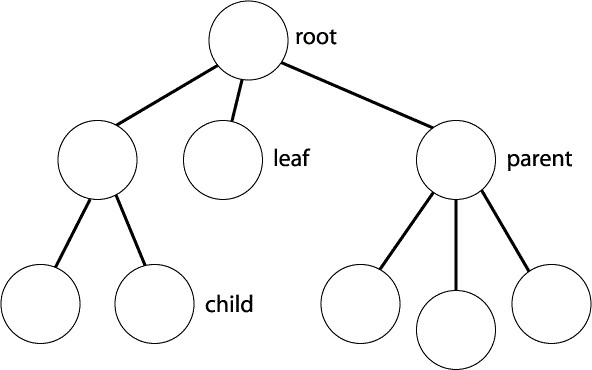
\includegraphics[width=0.8\linewidth]{img/xmlDiagram} 

}

\caption{Source: mysamplecode.com}\label{fig:unnamed-chunk-281}
\end{figure}

There are two major R packages for reading in XML data:

\begin{enumerate}
\def\labelenumi{\arabic{enumi}.}
\item
  \texttt{XML}
\item
  \texttt{xml2}
\end{enumerate}

\texttt{xml2} has all the basic functionality to get data into R. Reading XML data is generally tough since the structure of tags varies by data source! The \href{https://cran.r-project.org/web/packages/xml2/index.html}{\texttt{xml2}} core functions are:

\begin{longtable}[]{@{}ll@{}}
\toprule
\begin{minipage}[b]{0.22\columnwidth}\raggedright
Function\strut
\end{minipage} & \begin{minipage}[b]{0.72\columnwidth}\raggedright
Description\strut
\end{minipage}\tabularnewline
\midrule
\endhead
\begin{minipage}[t]{0.22\columnwidth}\raggedright
\texttt{read\_xml}\strut
\end{minipage} & \begin{minipage}[t]{0.72\columnwidth}\raggedright
Accepts string, file path, or url argument. Returns XML data object\strut
\end{minipage}\tabularnewline
\begin{minipage}[t]{0.22\columnwidth}\raggedright
\texttt{xml\_children}\strut
\end{minipage} & \begin{minipage}[t]{0.72\columnwidth}\raggedright
Returns list of elements downstream from current node\strut
\end{minipage}\tabularnewline
\begin{minipage}[t]{0.22\columnwidth}\raggedright
\texttt{xml\_parents}\strut
\end{minipage} & \begin{minipage}[t]{0.72\columnwidth}\raggedright
Returns list of all parent elements from current node\strut
\end{minipage}\tabularnewline
\begin{minipage}[t]{0.22\columnwidth}\raggedright
\texttt{xml\_contents}\strut
\end{minipage} & \begin{minipage}[t]{0.72\columnwidth}\raggedright
Returns list of contents from current node\strut
\end{minipage}\tabularnewline
\begin{minipage}[t]{0.22\columnwidth}\raggedright
\texttt{as\_list}\strut
\end{minipage} & \begin{minipage}[t]{0.72\columnwidth}\raggedright
Converts XML document or node set to equivalent R list\strut
\end{minipage}\tabularnewline
\bottomrule
\end{longtable}

\hypertarget{databases}{%
\subsection{Databases}\label{databases}}

A database is a collection of data, usually a bunch of 2D tables that have keys that connect them. The Database Management System (DBMS) controls how users interact with the database. There is a common and very useful Structured Query Language (SQL - pronounced ess-que-el or sequel) used by relational database management systems (RDBMS) for retrieving and combining datasets from a database.

An example of a relational database structure is given below. Notice there are keys that link different tables.

\begin{figure}

{\centering 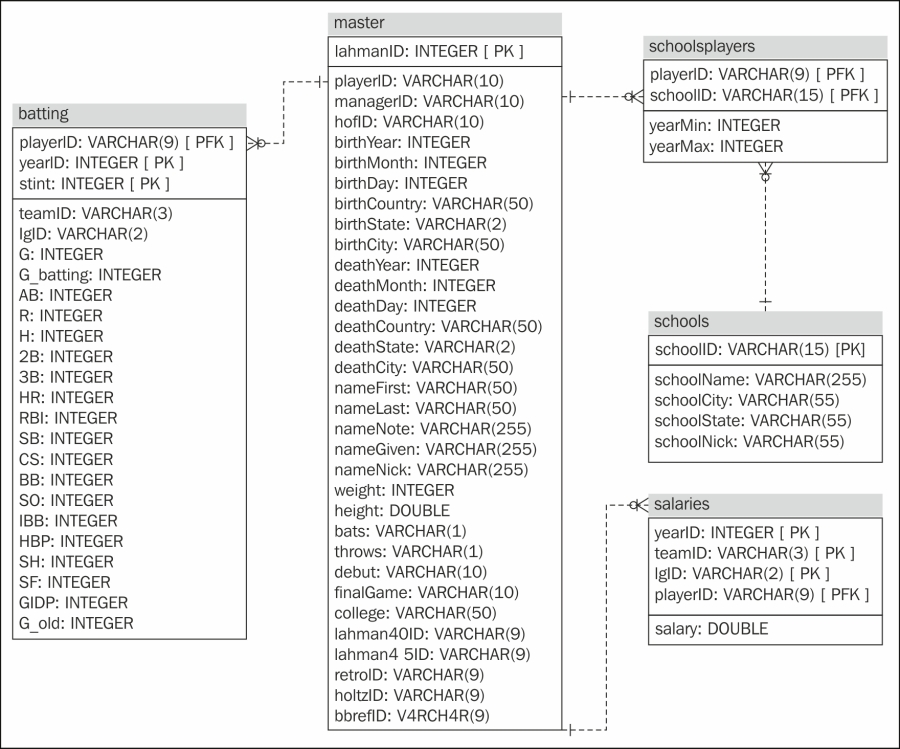
\includegraphics[width=0.8\linewidth]{img/lahman} 

}

\caption{Source: oreilly.com}\label{fig:unnamed-chunk-282}
\end{figure}

There are many popular RDBMS. Some are free and some are proprietary. These are often simply referred to as databases.

\begin{itemize}
\item
  Oracle - most popular (cross platform)
\item
  SQL Server - Microsoft product
\item
  DB2 - IBM product
\item
  MySQL (open source) - Not as many features but popular
\item
  PostgreSQL (open source)
\end{itemize}

Again there is a \href{http://www.sqltutorial.org/sql-cheat-sheet/}{Basic SQL language} that is constant across all these database types.

The common flow to connect to a database using R is:

\begin{enumerate}
\def\labelenumi{\arabic{enumi}.}
\tightlist
\item
  Connect to the database with \texttt{DBI::dbConnect()}\\
\end{enumerate}

\begin{itemize}
\tightlist
\item
  Need appropriate R package for database backend

  \begin{itemize}
  \tightlist
  \item
    \texttt{RSQLite::SQLite()} for RSQLite\\
  \item
    \texttt{RMySQL::MySQL()} for RMySQL\\
  \item
    \texttt{RPostgreSQL::PostgreSQL()} for RPostgreSQL\\
  \item
    \texttt{odbc::odbc()} for Open Database Connectivity\\
  \item
    \texttt{bigrquery::bigquery()} for google's bigQuery
  \end{itemize}
\end{itemize}

\begin{Shaded}
\begin{Highlighting}[]
\NormalTok{con <-}\StringTok{ }\NormalTok{DBI}\OperatorTok{::}\KeywordTok{dbConnect}\NormalTok{(RMySQL}\OperatorTok{::}\KeywordTok{MySQL}\NormalTok{(), }
  \DataTypeTok{host =} \StringTok{"hostname.website"}\NormalTok{,}
  \DataTypeTok{user =} \StringTok{"username"}\NormalTok{,}
  \DataTypeTok{password =}\NormalTok{ rstudioapi}\OperatorTok{::}\KeywordTok{askForPassword}\NormalTok{(}\StringTok{"DB password"}\NormalTok{)}
\NormalTok{)}
\end{Highlighting}
\end{Shaded}

\begin{enumerate}
\def\labelenumi{\arabic{enumi}.}
\setcounter{enumi}{1}
\tightlist
\item
  Use \texttt{tbl()} to reference a table in the database
\end{enumerate}

\begin{Shaded}
\begin{Highlighting}[]
\KeywordTok{tbl}\NormalTok{(con, }\StringTok{"name_of_table"}\NormalTok{)}
\end{Highlighting}
\end{Shaded}

\begin{enumerate}
\def\labelenumi{\arabic{enumi}.}
\setcounter{enumi}{2}
\tightlist
\item
  Query the database with \texttt{SQL} or \texttt{dplyr/dbplyr}
\end{enumerate}

There is much more about \href{https://db.rstudio.com/}{R Studio and Databases here}.

\hypertarget{apis}{%
\subsection{APIs}\label{apis}}

API stands for Application Programming Interfaces. This is essentially a defined method for asking for information from a computer. They are useful for getting data or allowing others to run a model you've built.

There are many open APIs. They usually just require you to register and obtain a key. Once you have a key you simply need to construct the proper URL to return the information you want from the API.

As a quick example we will query the Harry Potter database at \url{https://www.potterapi.com/}. There is a button on the top right where you can register and obtain a key.

\begin{center}
\includegraphics[width=0.8\linewidth]{img/HPAPI} \end{center}

The documentation for returning Harry Potter spells states:

\begin{verbatim}
+ All routes need to be prefixed with https://www.potterapi.com/v1/  

+ GET request: /spells returns all spells 

+ Key goes on the end  
\end{verbatim}

This tells us how to construct the appropriate URL. The \texttt{paste} and \texttt{paste0} functions are useful for combining strings (check their help).

\begin{Shaded}
\begin{Highlighting}[]
\NormalTok{baseURL <-}\StringTok{ "https://www.potterapi.com/v1/"}
\NormalTok{value <-}\StringTok{ "spells?"}
\NormalTok{key <-}\StringTok{ "key=$2a$10$UMvDCH.93fa2KOjKbJYkOOPMNzdzQpJ0gMnVEtcHzW5Ic04HUmcsa"}
\NormalTok{URL <-}\StringTok{ }\KeywordTok{paste0}\NormalTok{(baseURL, value, key)}
\NormalTok{URL}
\end{Highlighting}
\end{Shaded}

\begin{verbatim}
## [1] "https://www.potterapi.com/v1/spells?key=$2a$10$UMvDCH.93fa2KOjKbJYkOOPMNzdzQpJ0gMnVEtcHzW5Ic04HUmcsa"
\end{verbatim}

Now we use the \texttt{RCurl} package and the \texttt{getURL} function to ping the URL we just created. This will return the spell data set in JSON form as that is the default response format for this API.

\begin{Shaded}
\begin{Highlighting}[]
\NormalTok{spellData <-}\StringTok{ }\NormalTok{RCurl}\OperatorTok{::}\KeywordTok{getURL}\NormalTok{(URL)}
\end{Highlighting}
\end{Shaded}

This is a reasonably large string of information so we can just look at the first 100 characters using the \texttt{substr} function.

\begin{Shaded}
\begin{Highlighting}[]
\KeywordTok{substr}\NormalTok{(spellData, }\DecValTok{1}\NormalTok{, }\DecValTok{100}\NormalTok{) }
\end{Highlighting}
\end{Shaded}

\begin{verbatim}
## [1] "[{\"_id\":\"5b74ebd5fb6fc0739646754c\",\"spell\":\"Aberto\",\"type\":\"Charm\",\"effect\":\"opens objects\"},{\"_id\":"
\end{verbatim}

To convert this to a data frame we can use the \texttt{fromJSON} function in the \texttt{jsonlite} package. \texttt{tbl\_df} converts the dataframe to a \texttt{tibble} (for printing purposes).

\begin{Shaded}
\begin{Highlighting}[]
\NormalTok{spellDataDF <-}\StringTok{ }\NormalTok{jsonlite}\OperatorTok{::}\KeywordTok{fromJSON}\NormalTok{(spellData)}
\KeywordTok{tbl_df}\NormalTok{(spellDataDF)}
\end{Highlighting}
\end{Shaded}

\begin{verbatim}
## # A tibble: 151 x 5
##   `_id`                spell          type      effect                     `__v`
##   <chr>                <chr>          <chr>     <chr>                      <int>
## 1 5b74ebd5fb6fc073964~ Aberto         Charm     opens objects                 NA
## 2 5b74ecfa3228320021a~ Accio          Charm     Summons an object              0
## 3 5b74ed2f3228320021a~ Age Line       Enchantm~ Hides things from younger~     0
## 4 5b74ed453228320021a~ Aguamenti      Charm     shoots water from wand         0
## 5 5b74ed583228320021a~ Alarte Ascend~ Spell     shoots things high in the~     0
## # ... with 146 more rows
\end{verbatim}

Of course constructing URLs like this yourself isn't ideal. Languages like python have many packages to help you contact APIs without reading as much documentation. Unfortunately, R does not have a very mature collection of API packages. The article \href{https://www.programmableweb.com/news/how-to-access-any-restful-api-using-r-language/how-to/2017/07/21}{here} discusses accessing APIs generically with R. The same website gives a \href{https://www.programmableweb.com/category/all/apis}{list of APIs} that you might consider.

\hypertarget{data-manipulation-ideas}{%
\subsection{Data Manipulation Ideas}\label{data-manipulation-ideas}}

As you can see it isn't too difficult to bring well structured raw data into R. You should now have the basics of reading in delimited, Excel, SAS, SPSS, JSON, and XML data as well as how to connect to a database and contact an API. Once you have your data you may want to manipulate it in some way.

Often we want to grab only certain types of observations (filter rows).

\begin{center}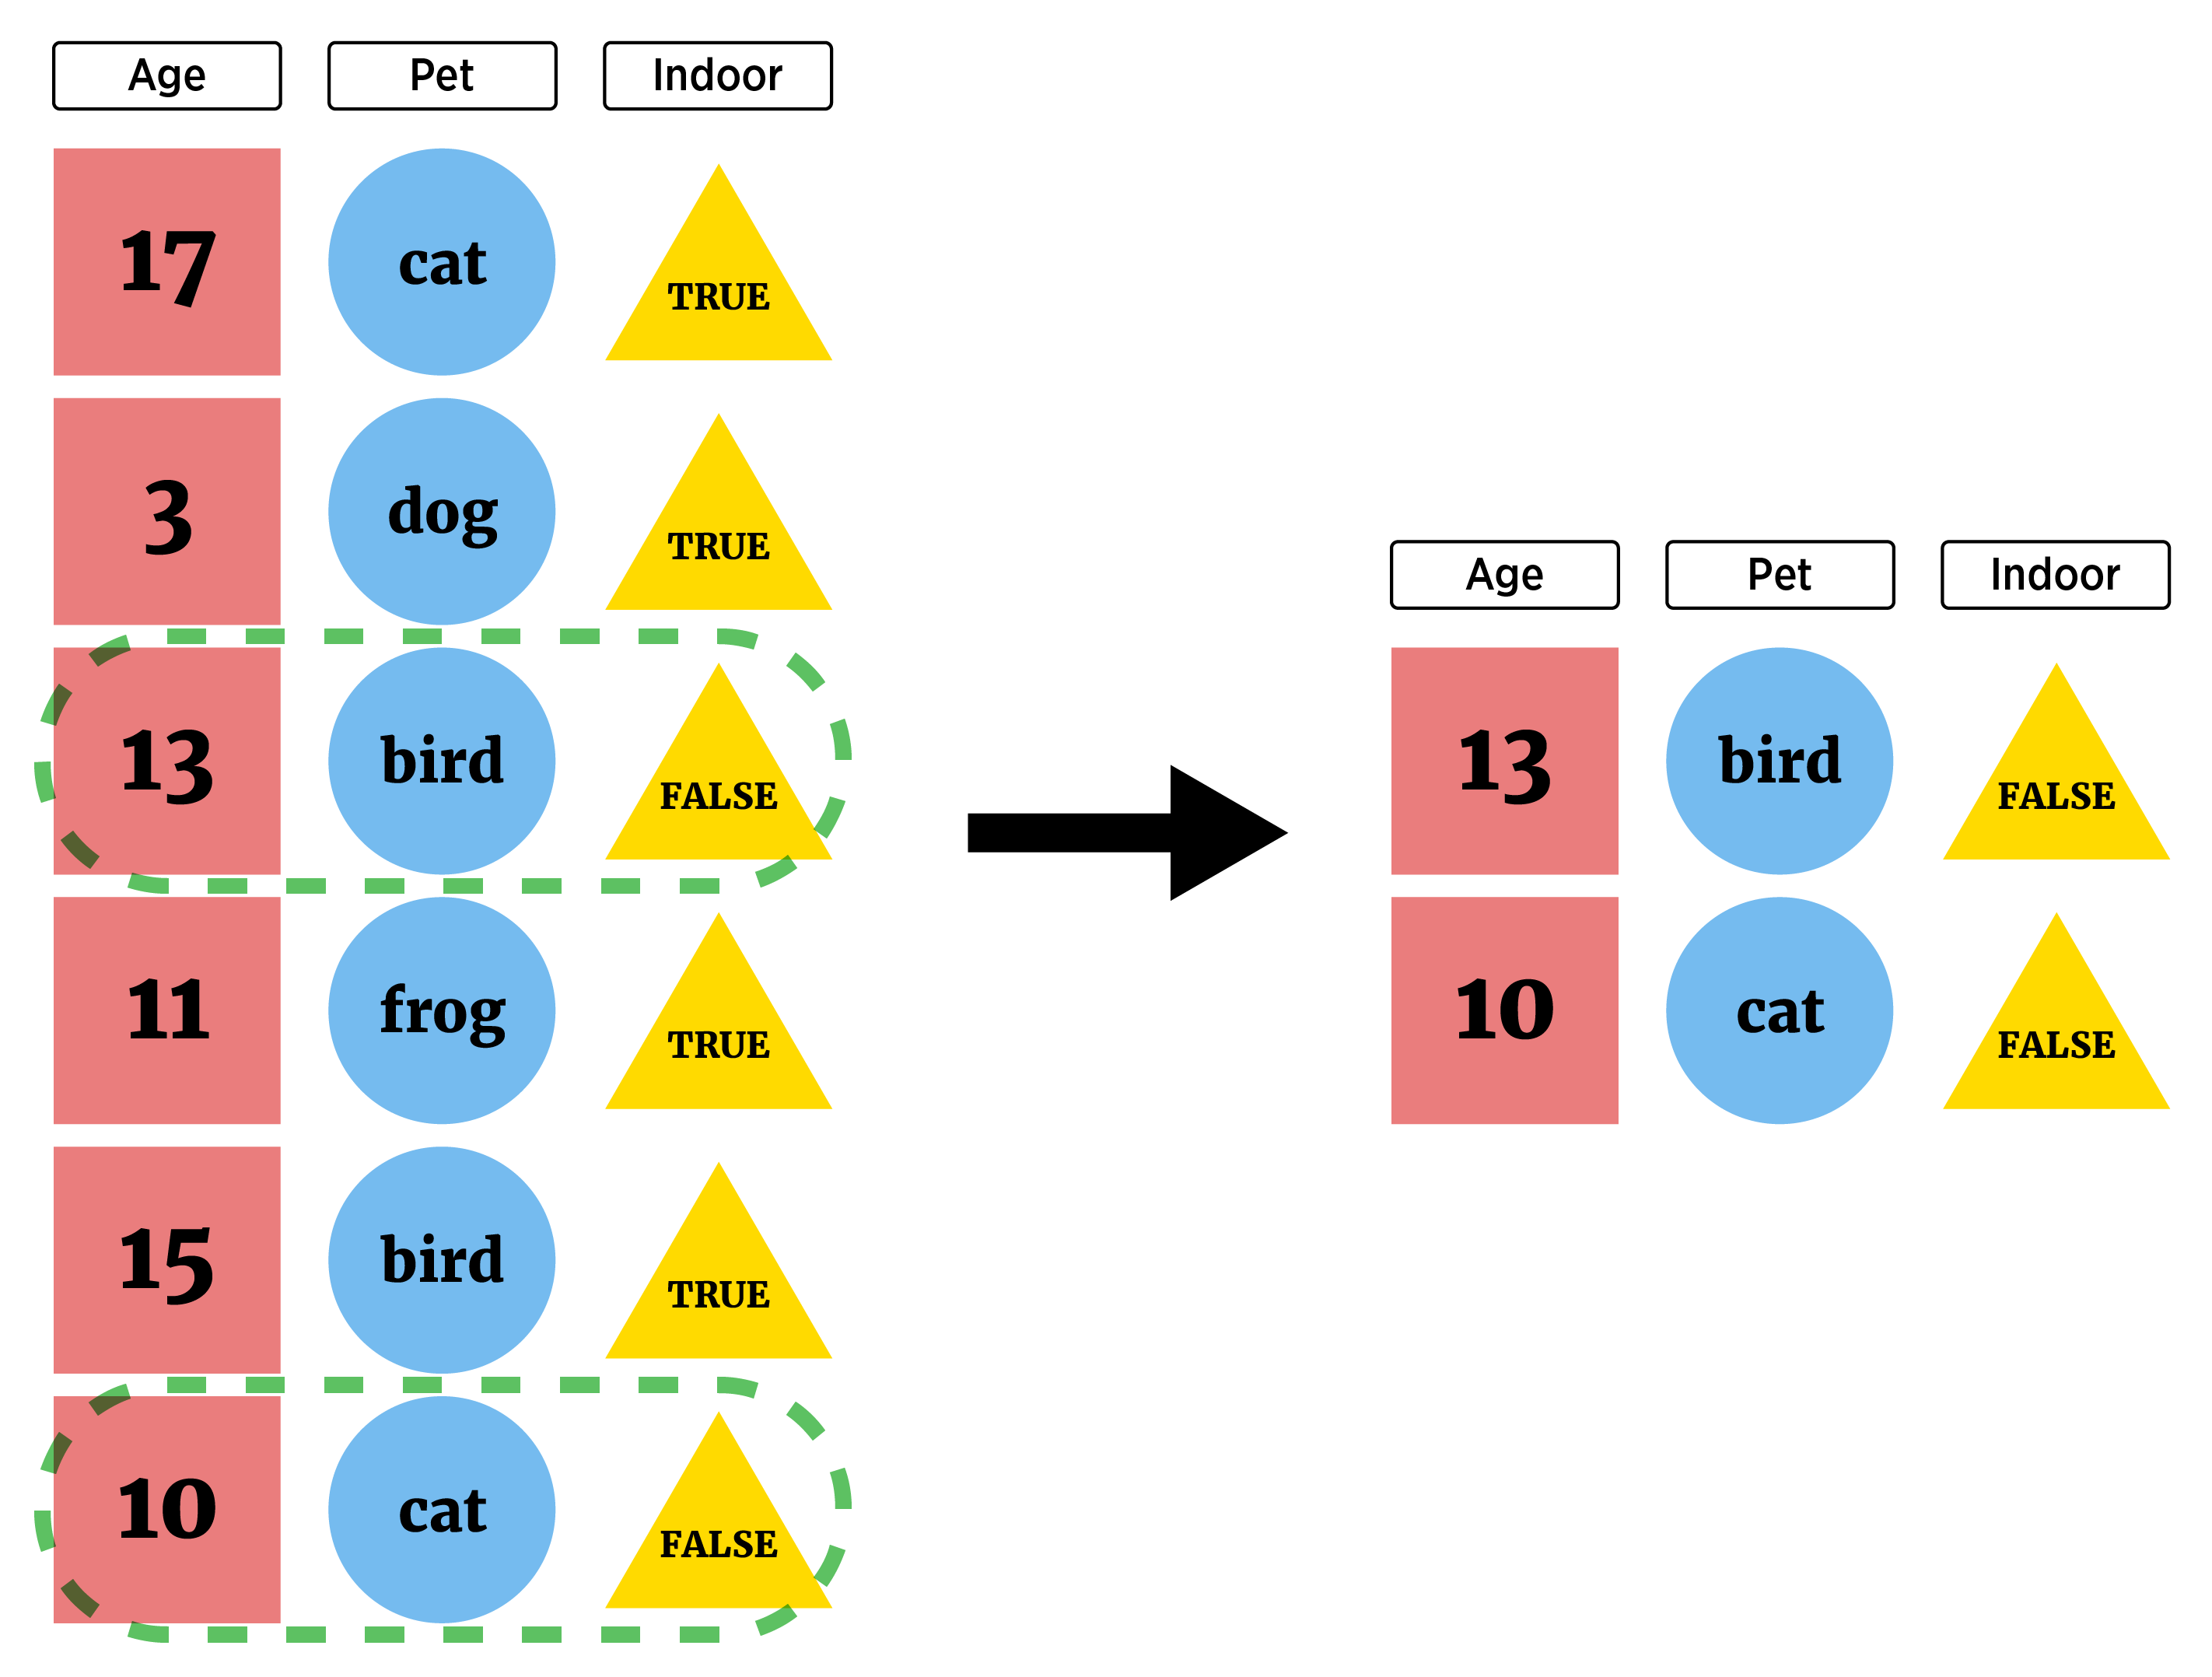
\includegraphics[width=0.8\linewidth]{img/filterVisualF} \end{center}

We also want to only look at only certain variables (select columns).

\begin{center}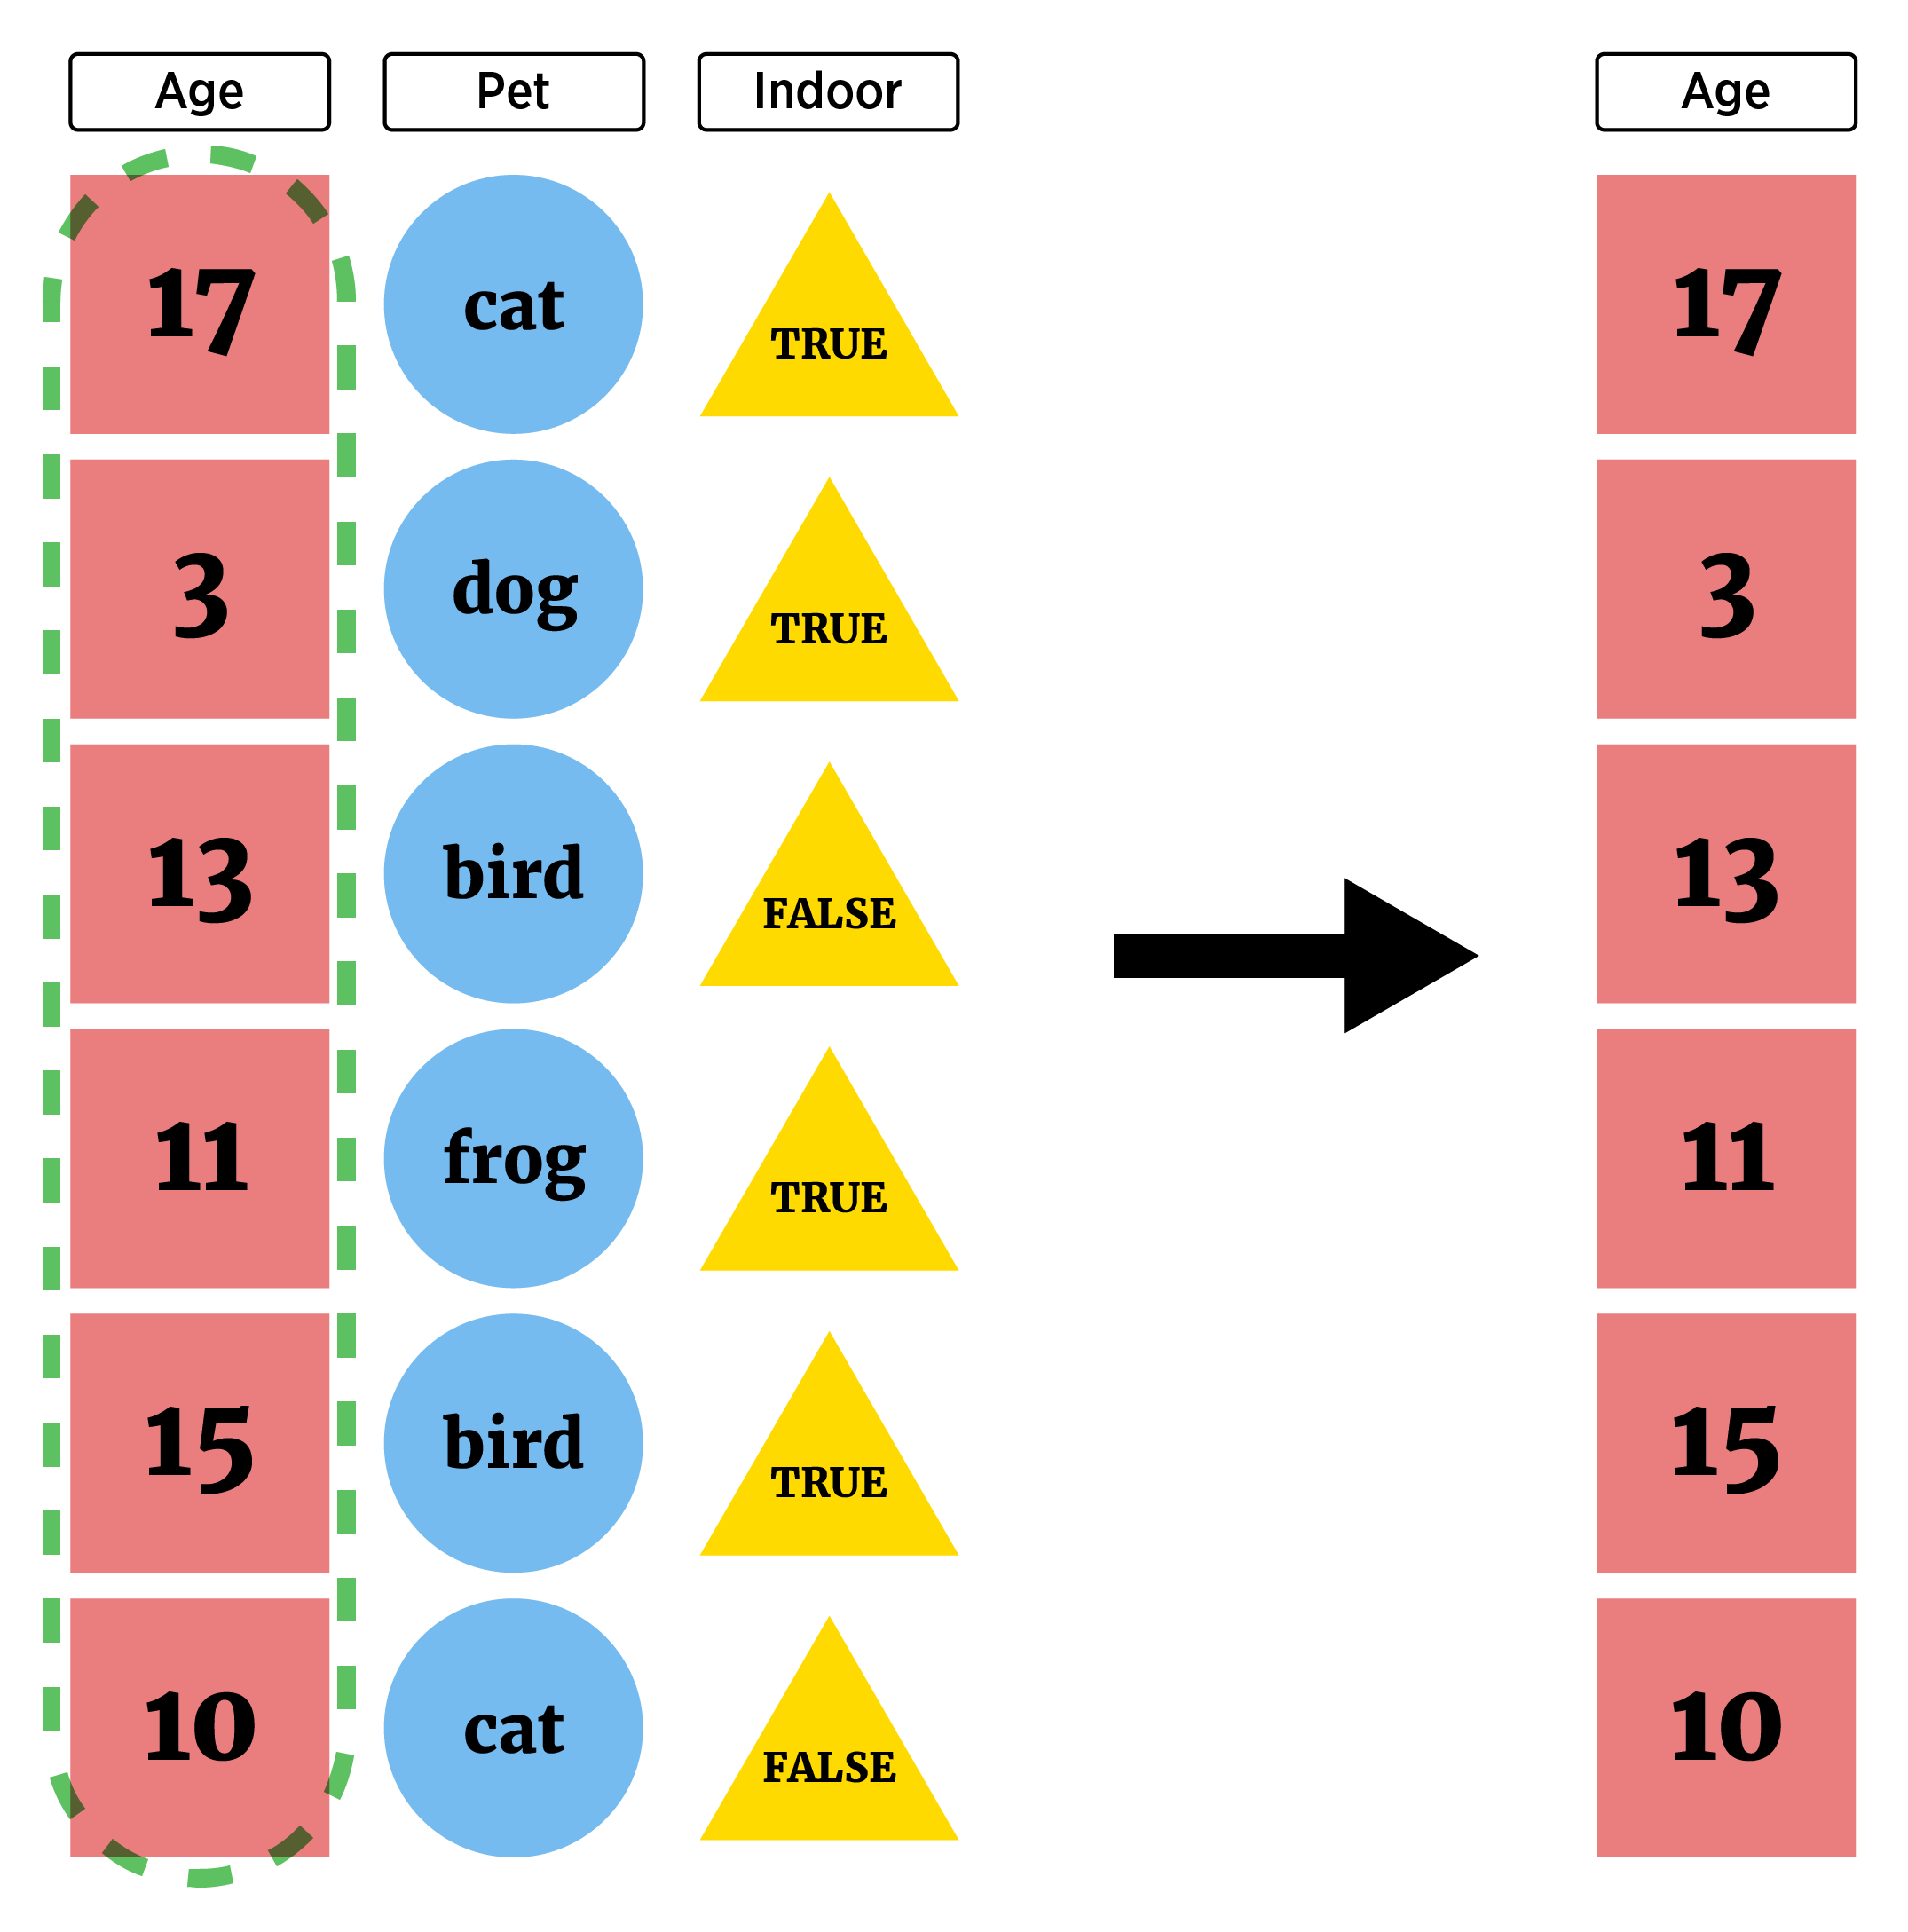
\includegraphics[width=0.7\linewidth]{img/selectVisualF} \end{center}

Other times we want to create new variables that may be functions of the data in the data set.

\begin{center}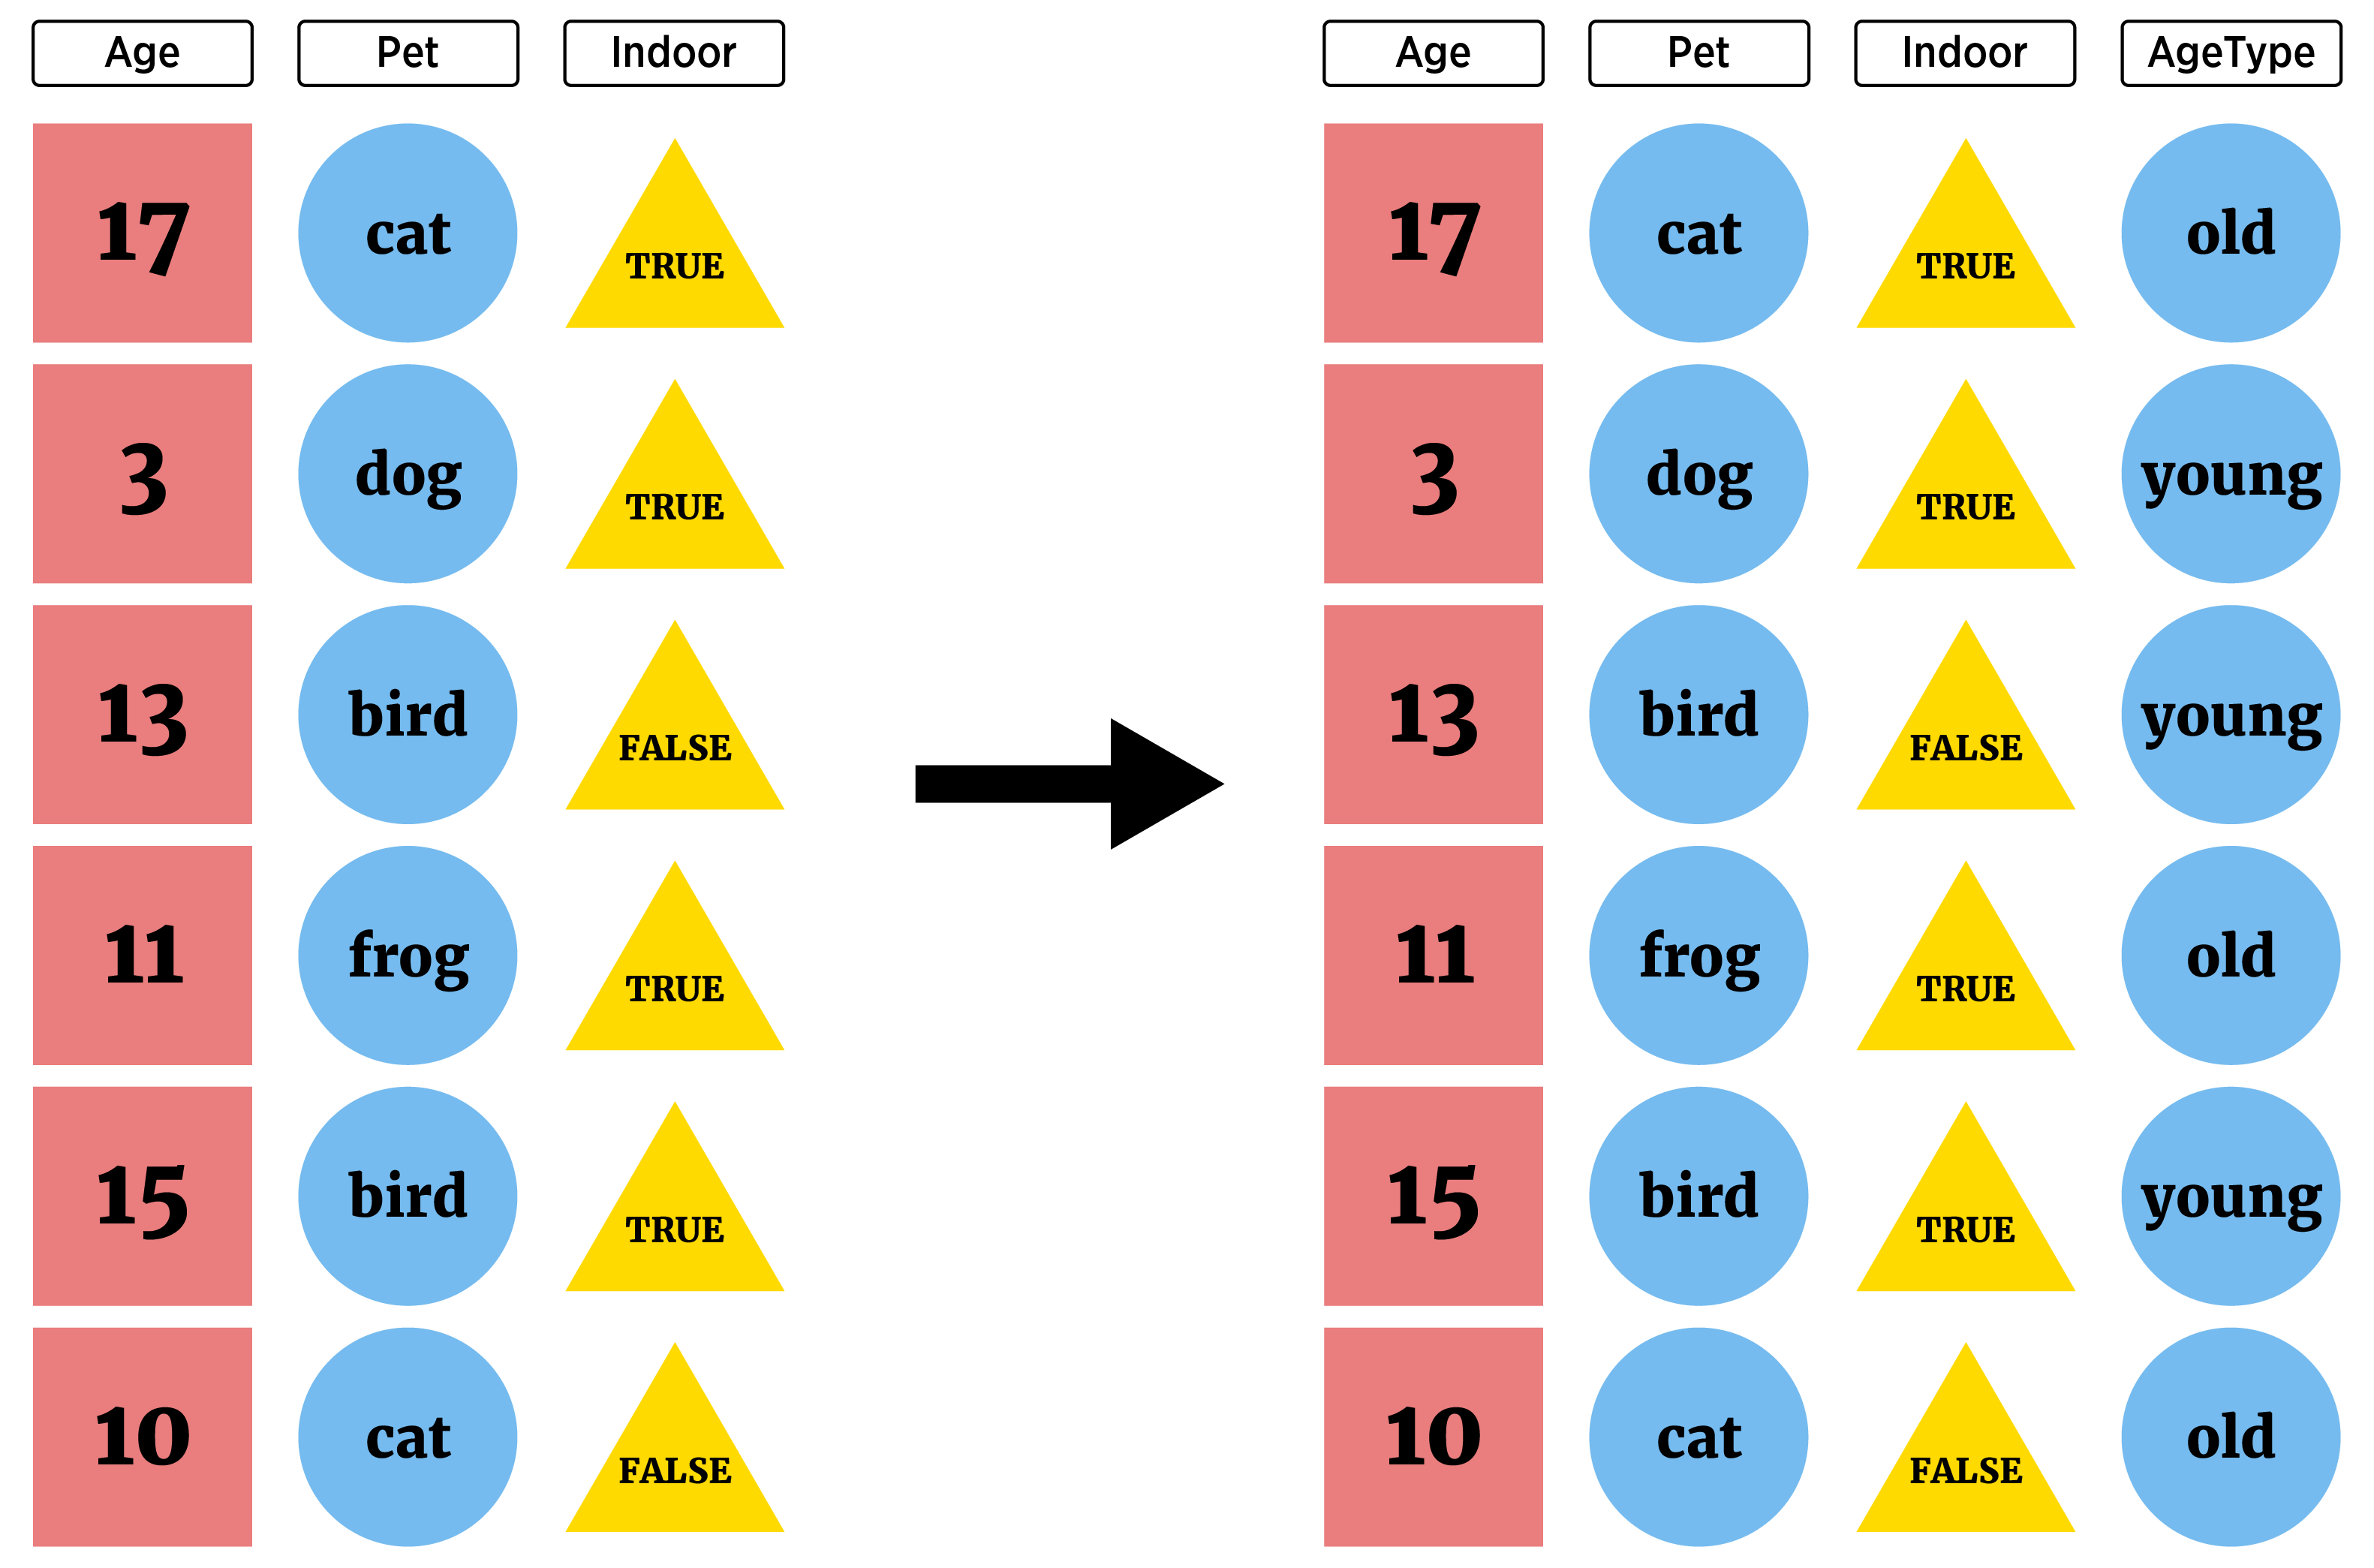
\includegraphics[width=0.8\linewidth]{img/createVarVisualF} \end{center}

When doing data manipulation it is vital to make your work reproducible! Traditionally documentation has been done through comments (\texttt{\#} in R) in your R script. This is being replaced by using a `Notebook' environment like R Markdown.

\hypertarget{documenting-with-markdown}{%
\subsection{Documenting with Markdown}\label{documenting-with-markdown}}

You may have heard of \href{http://jupyter.org/}{JUPYTER} notebooks. This is a program that allows you to weave plain text with formatting characters along side code. JUPYTER allows you to call Julia, Python, R, or SAS code (among others).

R Markdown is a built in notebook for R studio! A nice intro video is \href{https://vimeo.com/178485416}{available here}.

R Markdown is designed to be used in three ways (R for Data Science):

\begin{itemize}
\item
  Communicating to decision makers (focus on conclusions not code)
\item
  Collaborating with other data scientists (including future you!)
\item
  As environment to do data science (documents what you did and what you were thinking)
\end{itemize}

Most have heard of HTML or HyperText Mark-up Language. This is really just plain text that a web browser like firefox interprets and renders. Markdown is a specific markup language that has easier syntax but is not as powerful. Any plain text file can be used although the .Rmd extension associates the file with R Studio.

RStudio makes it easy to create a Markdown document.

\begin{center}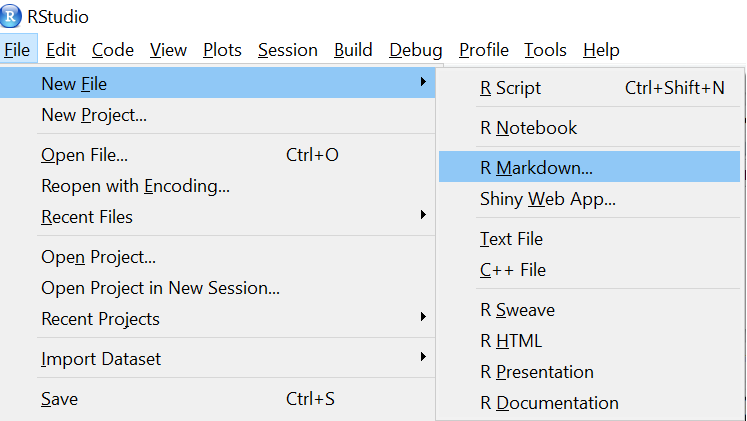
\includegraphics[width=0.75\linewidth]{img/startMD} \end{center}

You can create many commonly used types of output including HTML, PDF, Word, and HTML slides.

\begin{center}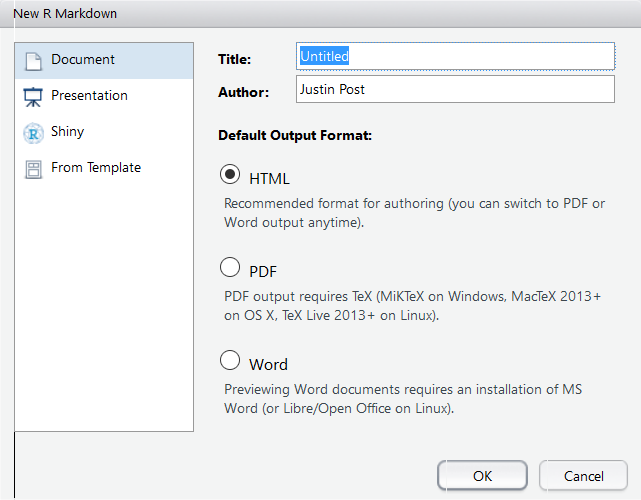
\includegraphics[width=0.65\linewidth]{img/startMDDoc} \end{center}

An R Markdown file contains three important types of content:

\begin{enumerate}
\def\labelenumi{\arabic{enumi}.}
\item
  (Optional) YAML header surrounded by \texttt{-\/-\/-}s
\item
  Chunks of R code
\item
  Text mixed with simple text formatting instructions
\end{enumerate}

The YAML header defines settings for document:

\begin{verbatim}
---
title: "Untitled"
author: "First Last"
date: "xxxx"
output: html_document
---
\end{verbatim}

The hot key combination of CTRL/CMD + Shift + k `knits' (or creates the output type) via this information.

Code Chunks can contain any R code. These can be started by typing ```\{r\} out or with CTRL/CMD + Alt + I. This code will be executed when document is created and the chunks will be evaulated sequentially. Options can be specified on individual code chunks to hide their code or output (among other things).

Below you'll see plain text with markdown sytnax included:

\begin{verbatim}
##R Markdown

This is an R Markdown document. Markdown is a simple formatting syntax
for authoring HTML, PDF, and MS Word documents. For more details on
using R Markdown see <http://rmarkdown.rstudio.com>.

When you click the **Knit** button a document will be generated that
includes both content as well as the output of any embedded R code
chunks within the document. 
\end{verbatim}

When the file is created \texttt{\#\#} becomes a header, ``\textless{}\ldots{}\textgreater{}'' a link, and \texttt{**Knit**} bold font.

You can learn much more about how to use R Markdown with this handy \href{https://www.rstudio.com/wp-content/uploads/2015/03/rmarkdown-reference.pdf}{cheat sheet}.

The key idea here is that you can easily write down your thought process and document all of the changes you make to your data. This creates a reproducible final product!

\hypertarget{logical-statements}{%
\subsection{Logical Statements}\label{logical-statements}}

Our current goal is to subset rows or columns of a dataset.

\begin{center}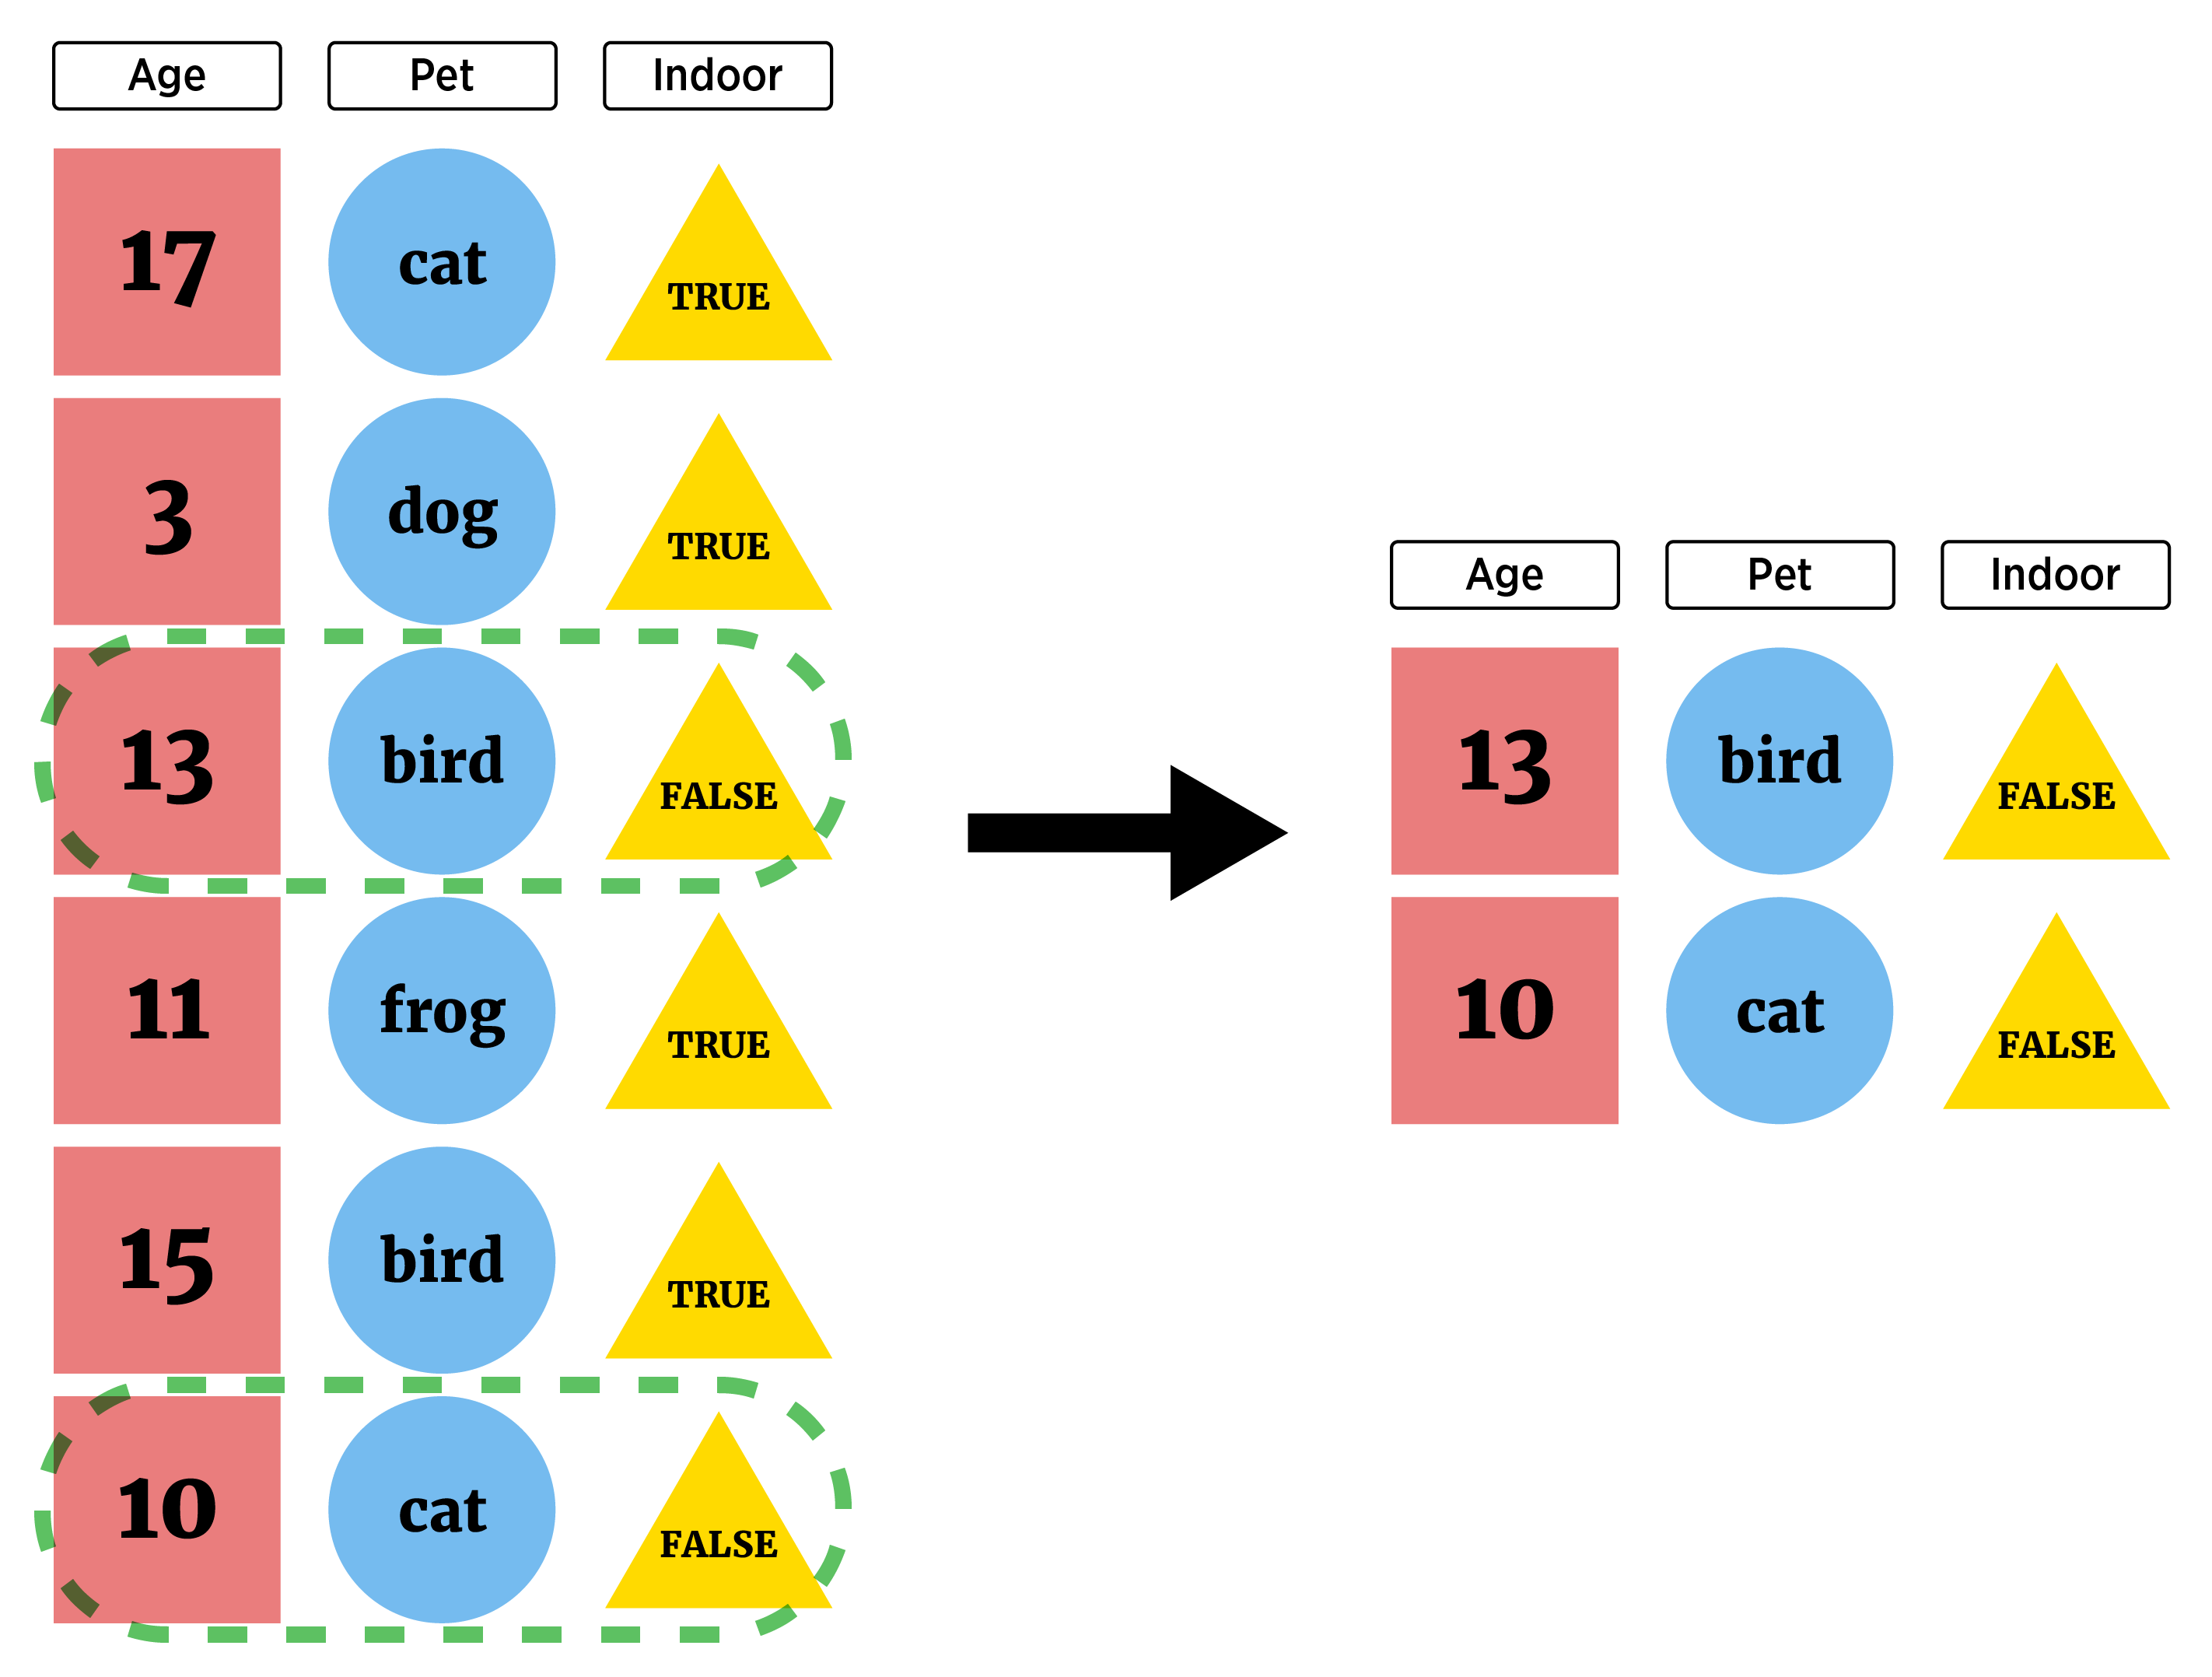
\includegraphics[width=0.8\linewidth]{img/filterVisualF} \end{center}

To do this efficiently we need to learn about logical statements. A logical statement is a comparison that resolves as \texttt{TRUE} or \texttt{FALSE}. R has all of the standard comparison operators:

\begin{itemize}
\tightlist
\item
  \texttt{==} equal to
\item
  \texttt{!=} not equal to
\item
  \texttt{\textless{}}, \texttt{\textless{}=}, \texttt{\textgreater{}}, \texttt{\textgreater{}=} less than (or equal) and greater than (or equal)
\end{itemize}

\begin{Shaded}
\begin{Highlighting}[]
\StringTok{"hi"} \OperatorTok{==}\StringTok{ " hi"} \CommentTok{#== is comparison}
\end{Highlighting}
\end{Shaded}

\begin{verbatim}
## [1] FALSE
\end{verbatim}

\begin{Shaded}
\begin{Highlighting}[]
\StringTok{"hi"} \OperatorTok{==}\StringTok{ "hi"}
\end{Highlighting}
\end{Shaded}

\begin{verbatim}
## [1] TRUE
\end{verbatim}

\begin{Shaded}
\begin{Highlighting}[]
\DecValTok{4} \OperatorTok{>=}\StringTok{ }\DecValTok{1}
\end{Highlighting}
\end{Shaded}

\begin{verbatim}
## [1] TRUE
\end{verbatim}

\begin{Shaded}
\begin{Highlighting}[]
\DecValTok{4} \OperatorTok{!=}\StringTok{ }\DecValTok{1}
\end{Highlighting}
\end{Shaded}

\begin{verbatim}
## [1] TRUE
\end{verbatim}

Sometimes we see issues due to a loss of precision when doing mathematical operations.

\begin{Shaded}
\begin{Highlighting}[]
\KeywordTok{sqrt}\NormalTok{(}\DecValTok{3}\NormalTok{)}\OperatorTok{^}\DecValTok{2}  \OperatorTok{==}\StringTok{ }\DecValTok{3}
\end{Highlighting}
\end{Shaded}

\begin{verbatim}
## [1] FALSE
\end{verbatim}

The \texttt{near} function from the \texttt{dplyr} package can help with this type of situation.

\begin{Shaded}
\begin{Highlighting}[]
\NormalTok{dplyr}\OperatorTok{::}\KeywordTok{near}\NormalTok{(}\KeywordTok{sqrt}\NormalTok{(}\DecValTok{3}\NormalTok{)}\OperatorTok{^}\DecValTok{2}\NormalTok{, }\DecValTok{3}\NormalTok{)}
\end{Highlighting}
\end{Shaded}

\begin{verbatim}
## [1] TRUE
\end{verbatim}

Another common way to do a logical statement in R is to use an \texttt{is.} family function.

\begin{Shaded}
\begin{Highlighting}[]
\KeywordTok{is.numeric}\NormalTok{(}\StringTok{"Word"}\NormalTok{)}
\end{Highlighting}
\end{Shaded}

\begin{verbatim}
## [1] FALSE
\end{verbatim}

\begin{Shaded}
\begin{Highlighting}[]
\KeywordTok{is.numeric}\NormalTok{(}\DecValTok{10}\NormalTok{)}
\end{Highlighting}
\end{Shaded}

\begin{verbatim}
## [1] TRUE
\end{verbatim}

\begin{Shaded}
\begin{Highlighting}[]
\KeywordTok{is.character}\NormalTok{(}\StringTok{"10"}\NormalTok{)}
\end{Highlighting}
\end{Shaded}

\begin{verbatim}
## [1] TRUE
\end{verbatim}

\begin{Shaded}
\begin{Highlighting}[]
\KeywordTok{is.na}\NormalTok{(}\KeywordTok{c}\NormalTok{(}\DecValTok{1}\OperatorTok{:}\DecValTok{2}\NormalTok{, }\OtherTok{NA}\NormalTok{, }\DecValTok{3}\NormalTok{))}
\end{Highlighting}
\end{Shaded}

\begin{verbatim}
## [1] FALSE FALSE  TRUE FALSE
\end{verbatim}

\begin{Shaded}
\begin{Highlighting}[]
\KeywordTok{is.matrix}\NormalTok{(}\KeywordTok{c}\NormalTok{(}\StringTok{"hello"}\NormalTok{, }\StringTok{"world"}\NormalTok{))}
\end{Highlighting}
\end{Shaded}

\begin{verbatim}
## [1] FALSE
\end{verbatim}

How do we use logical statements to subset our data? Logical vectors can be used for indexing an R object. The concept is:

\begin{itemize}
\tightlist
\item
  Feed index a vector of \texttt{TRUE}/\texttt{FALSE} or \texttt{0}/\texttt{1} values\\
\item
  R will return elements where \texttt{TRUE} or \texttt{1} occurred
\end{itemize}

Let's subset the built-in \texttt{iris} data set. First we'll convert it to a \texttt{tibble} so it prints nicely.

\begin{Shaded}
\begin{Highlighting}[]
\NormalTok{iris <-}\StringTok{ }\KeywordTok{tbl_df}\NormalTok{(iris)}
\NormalTok{iris}
\end{Highlighting}
\end{Shaded}

Now, we can create an indexing vector corresponding to some condition of interest. For instance, we may want to only look at the Species `setosa' flowers.

\begin{Shaded}
\begin{Highlighting}[]
\NormalTok{iris}\OperatorTok{$}\NormalTok{Species }\OperatorTok{==}\StringTok{ "setosa"} \CommentTok{#vector indicating setosa values}
\end{Highlighting}
\end{Shaded}

\begin{verbatim}
##   [1]  TRUE  TRUE  TRUE  TRUE  TRUE  TRUE  TRUE  TRUE  TRUE  TRUE  TRUE  TRUE
##  [13]  TRUE  TRUE  TRUE  TRUE  TRUE  TRUE  TRUE  TRUE  TRUE  TRUE  TRUE  TRUE
##  [25]  TRUE  TRUE  TRUE  TRUE  TRUE  TRUE  TRUE  TRUE  TRUE  TRUE  TRUE  TRUE
##  [37]  TRUE  TRUE  TRUE  TRUE  TRUE  TRUE  TRUE  TRUE  TRUE  TRUE  TRUE  TRUE
##  [49]  TRUE  TRUE FALSE FALSE FALSE FALSE FALSE FALSE FALSE FALSE FALSE FALSE
##  [61] FALSE FALSE FALSE FALSE FALSE FALSE FALSE FALSE FALSE FALSE FALSE FALSE
##  [73] FALSE FALSE FALSE FALSE FALSE FALSE FALSE FALSE FALSE FALSE FALSE FALSE
##  [85] FALSE FALSE FALSE FALSE FALSE FALSE FALSE FALSE FALSE FALSE FALSE FALSE
##  [97] FALSE FALSE FALSE FALSE
##  [ reached getOption("max.print") -- omitted 50 entries ]
\end{verbatim}

Now we can feed this in as our row index to the \texttt{{[}} function. Remember for rectangular data the first index you give refers to the rows and the second to columns.

\begin{Shaded}
\begin{Highlighting}[]
\NormalTok{iris[iris}\OperatorTok{$}\NormalTok{Species }\OperatorTok{==}\StringTok{ "setosa"}\NormalTok{, ]}
\end{Highlighting}
\end{Shaded}

\begin{verbatim}
##    Sepal.Length Sepal.Width Petal.Length Petal.Width Species
## 1           5.1         3.5          1.4         0.2  setosa
## 2           4.9         3.0          1.4         0.2  setosa
## 3           4.7         3.2          1.3         0.2  setosa
## 4           4.6         3.1          1.5         0.2  setosa
## 5           5.0         3.6          1.4         0.2  setosa
## 6           5.4         3.9          1.7         0.4  setosa
## 7           4.6         3.4          1.4         0.3  setosa
## 8           5.0         3.4          1.5         0.2  setosa
## 9           4.4         2.9          1.4         0.2  setosa
## 10          4.9         3.1          1.5         0.1  setosa
## 11          5.4         3.7          1.5         0.2  setosa
## 12          4.8         3.4          1.6         0.2  setosa
## 13          4.8         3.0          1.4         0.1  setosa
## 14          4.3         3.0          1.1         0.1  setosa
## 15          5.8         4.0          1.2         0.2  setosa
## 16          5.7         4.4          1.5         0.4  setosa
## 17          5.4         3.9          1.3         0.4  setosa
## 18          5.1         3.5          1.4         0.3  setosa
## 19          5.7         3.8          1.7         0.3  setosa
## 20          5.1         3.8          1.5         0.3  setosa
##  [ reached 'max' / getOption("max.print") -- omitted 30 rows ]
\end{verbatim}

Rather than use \texttt{{[}}, a base R function called \texttt{subset} can be used.

\begin{Shaded}
\begin{Highlighting}[]
\KeywordTok{subset}\NormalTok{(iris, Species }\OperatorTok{==}\StringTok{ "setosa"}\NormalTok{)}
\end{Highlighting}
\end{Shaded}

\begin{verbatim}
##    Sepal.Length Sepal.Width Petal.Length Petal.Width Species
## 1           5.1         3.5          1.4         0.2  setosa
## 2           4.9         3.0          1.4         0.2  setosa
## 3           4.7         3.2          1.3         0.2  setosa
## 4           4.6         3.1          1.5         0.2  setosa
## 5           5.0         3.6          1.4         0.2  setosa
## 6           5.4         3.9          1.7         0.4  setosa
## 7           4.6         3.4          1.4         0.3  setosa
## 8           5.0         3.4          1.5         0.2  setosa
## 9           4.4         2.9          1.4         0.2  setosa
## 10          4.9         3.1          1.5         0.1  setosa
## 11          5.4         3.7          1.5         0.2  setosa
## 12          4.8         3.4          1.6         0.2  setosa
## 13          4.8         3.0          1.4         0.1  setosa
## 14          4.3         3.0          1.1         0.1  setosa
## 15          5.8         4.0          1.2         0.2  setosa
## 16          5.7         4.4          1.5         0.4  setosa
## 17          5.4         3.9          1.3         0.4  setosa
## 18          5.1         3.5          1.4         0.3  setosa
## 19          5.7         3.8          1.7         0.3  setosa
## 20          5.1         3.8          1.5         0.3  setosa
##  [ reached 'max' / getOption("max.print") -- omitted 30 rows ]
\end{verbatim}

This function works quite well but we want to work in the tidyverse. The \texttt{filter} function from the \texttt{dplyr} package (installed with \texttt{tidyverse}) will be our function of choice. For \texttt{filter} the first argument is the data frame (or tibble) and the second is the logical statement used for indexing the rows.

\begin{Shaded}
\begin{Highlighting}[]
\KeywordTok{filter}\NormalTok{(iris, Species }\OperatorTok{==}\StringTok{ "setosa"}\NormalTok{)}
\end{Highlighting}
\end{Shaded}

\begin{verbatim}
##    Sepal.Length Sepal.Width Petal.Length Petal.Width Species
## 1           5.1         3.5          1.4         0.2  setosa
## 2           4.9         3.0          1.4         0.2  setosa
## 3           4.7         3.2          1.3         0.2  setosa
## 4           4.6         3.1          1.5         0.2  setosa
## 5           5.0         3.6          1.4         0.2  setosa
## 6           5.4         3.9          1.7         0.4  setosa
## 7           4.6         3.4          1.4         0.3  setosa
## 8           5.0         3.4          1.5         0.2  setosa
## 9           4.4         2.9          1.4         0.2  setosa
## 10          4.9         3.1          1.5         0.1  setosa
## 11          5.4         3.7          1.5         0.2  setosa
## 12          4.8         3.4          1.6         0.2  setosa
## 13          4.8         3.0          1.4         0.1  setosa
## 14          4.3         3.0          1.1         0.1  setosa
## 15          5.8         4.0          1.2         0.2  setosa
## 16          5.7         4.4          1.5         0.4  setosa
## 17          5.4         3.9          1.3         0.4  setosa
## 18          5.1         3.5          1.4         0.3  setosa
## 19          5.7         3.8          1.7         0.3  setosa
## 20          5.1         3.8          1.5         0.3  setosa
##  [ reached 'max' / getOption("max.print") -- omitted 30 rows ]
\end{verbatim}

Often we'll want to subset based on more than one condition. These can be created using standard logical operators. In R these are:

\begin{itemize}
\tightlist
\item
  \texttt{\&} `and'
\item
  \texttt{\textbar{}} `or'
\end{itemize}

\begin{longtable}[]{@{}llll@{}}
\toprule
Operator & A,B true & A true, B false & A,B false\tabularnewline
\midrule
\endhead
\texttt{\&} & \texttt{A\ \&\ B\ =\ TRUE} & \texttt{A\ \&\ B\ =\ FALSE} & \texttt{A\ \&\ B\ =\ FALSE}\tabularnewline
\texttt{\textbar{}} & \texttt{A\ \textbar{}\ B\ =\ TRUE} & \texttt{A\ \textbar{}\ B\ =\ TRUE} & \texttt{A\ \textbar{}\ B\ =\ FALSE}\tabularnewline
\bottomrule
\end{longtable}

For the most part we'll want to use the single \texttt{\&} or \texttt{\textbar{}}. \texttt{\&\&} and \texttt{\textbar{}\textbar{}} are alternatives that only look at only first comparison done (if given a vector of comparisons).

A quick example of the compound logical syntax is given below. Parenthesis are not necessary but are quite useful to keep things straight! Here we generate 10 random values between 0 and 1 (\texttt{set.seed} just starts the random number generator at a specific spot so we can get the same 10 values each time we create this document!). We use \texttt{\textbar{}} to return TRUE if the randomly generated value is either below 0.25 or above 0.75.

\begin{Shaded}
\begin{Highlighting}[]
\KeywordTok{set.seed}\NormalTok{(}\DecValTok{3}\NormalTok{)}
\NormalTok{x <-}\StringTok{ }\KeywordTok{runif}\NormalTok{(}\DataTypeTok{n =} \DecValTok{10}\NormalTok{, }\DataTypeTok{min =} \DecValTok{0}\NormalTok{, }\DataTypeTok{max =} \DecValTok{1}\NormalTok{)}
\NormalTok{x}
\end{Highlighting}
\end{Shaded}

\begin{verbatim}
##  [1] 0.1680415 0.8075164 0.3849424 0.3277343 0.6021007 0.6043941 0.1246334
##  [8] 0.2946009 0.5776099 0.6309793
\end{verbatim}

\begin{Shaded}
\begin{Highlighting}[]
\NormalTok{(x }\OperatorTok{<}\StringTok{ }\FloatTok{0.25}\NormalTok{) }\OperatorTok{|}\StringTok{ }\NormalTok{(x }\OperatorTok{>}\StringTok{ }\FloatTok{0.75}\NormalTok{)}
\end{Highlighting}
\end{Shaded}

\begin{verbatim}
##  [1]  TRUE  TRUE FALSE FALSE FALSE FALSE  TRUE FALSE FALSE FALSE
\end{verbatim}

With this kind of syntax we can now create an indexing vector to only pull out large petal setosa flowers:

\begin{Shaded}
\begin{Highlighting}[]
\NormalTok{(iris}\OperatorTok{$}\NormalTok{Petal.Length }\OperatorTok{>}\StringTok{ }\FloatTok{1.5}\NormalTok{) }\OperatorTok{&}\StringTok{ }\NormalTok{(iris}\OperatorTok{$}\NormalTok{Petal.Width }\OperatorTok{>}\StringTok{ }\FloatTok{0.3}\NormalTok{) }\OperatorTok{&}\StringTok{ }\NormalTok{(iris}\OperatorTok{$}\NormalTok{Species }\OperatorTok{==}\StringTok{ "setosa"}\NormalTok{)}
\end{Highlighting}
\end{Shaded}

\begin{verbatim}
##   [1] FALSE FALSE FALSE FALSE FALSE  TRUE FALSE FALSE FALSE FALSE FALSE FALSE
##  [13] FALSE FALSE FALSE FALSE FALSE FALSE FALSE FALSE FALSE FALSE FALSE  TRUE
##  [25] FALSE FALSE  TRUE FALSE FALSE FALSE FALSE FALSE FALSE FALSE FALSE FALSE
##  [37] FALSE FALSE FALSE FALSE FALSE FALSE FALSE  TRUE  TRUE FALSE FALSE FALSE
##  [49] FALSE FALSE FALSE FALSE FALSE FALSE FALSE FALSE FALSE FALSE FALSE FALSE
##  [61] FALSE FALSE FALSE FALSE FALSE FALSE FALSE FALSE FALSE FALSE FALSE FALSE
##  [73] FALSE FALSE FALSE FALSE FALSE FALSE FALSE FALSE FALSE FALSE FALSE FALSE
##  [85] FALSE FALSE FALSE FALSE FALSE FALSE FALSE FALSE FALSE FALSE FALSE FALSE
##  [97] FALSE FALSE FALSE FALSE
##  [ reached getOption("max.print") -- omitted 50 entries ]
\end{verbatim}

Using this in the filter function we return only a few observations corresponding to our condition.

\begin{Shaded}
\begin{Highlighting}[]
\KeywordTok{filter}\NormalTok{(iris, (Petal.Length }\OperatorTok{>}\StringTok{ }\FloatTok{1.5}\NormalTok{) }\OperatorTok{&}\StringTok{ }\NormalTok{(Petal.Width }\OperatorTok{>}\StringTok{ }\FloatTok{0.3}\NormalTok{) }\OperatorTok{&}\StringTok{ }
\StringTok{         }\NormalTok{(Species }\OperatorTok{==}\StringTok{ "setosa"}\NormalTok{))}
\end{Highlighting}
\end{Shaded}

\begin{verbatim}
##   Sepal.Length Sepal.Width Petal.Length Petal.Width Species
## 1          5.4         3.9          1.7         0.4  setosa
## 2          5.1         3.3          1.7         0.5  setosa
## 3          5.0         3.4          1.6         0.4  setosa
## 4          5.0         3.5          1.6         0.6  setosa
## 5          5.1         3.8          1.9         0.4  setosa
\end{verbatim}

\hypertarget{dplyr}{%
\subsection{\texorpdfstring{\texttt{dplyr}}{dplyr}}\label{dplyr}}

The tidyverse has many useful packages for common data manipulation tasks. Make sure \texttt{library(tidyverse)} has been run when working through this section!\\
Two major packages for data manipulation are:

-\texttt{dplry} package made for most standard data manipulation tasks

\begin{itemize}
\tightlist
\item
  \texttt{tidyr} package reshapes data (wide and long format, split columns, etc)
\end{itemize}

This section focuses on the most useful functions from the \texttt{dplyr} package:

\begin{itemize}
\tightlist
\item
  \texttt{tbl\_df()} - convert data frame to one with better printing\\
\item
  \texttt{filter()} - subset rows\\
\item
  \texttt{arrange()} - reorder rows\\
\item
  \texttt{select()} - subset columns\\
\item
  \texttt{rename()} - rename columns
\end{itemize}

Later we'll look at

\begin{itemize}
\tightlist
\item
  \texttt{mutate()} - add newly created column\\
\item
  \texttt{transmute()} - create new variable\\
\item
  \texttt{group\_by()} - group rows by a variable\\
\item
  \texttt{summarise()} - apply basic function to data
\end{itemize}

One really nice thing about the functions in the tidyverse is that the syntax is mostly consistent (save \texttt{ggplot2}). The basic syntax is

\texttt{function(tibble,\ actions,\ ...)}

Let's get started! We've seen \texttt{tbl\_df} a few times. This function converts a data frame to one with better printing and no simplification. To use it we can simply `wrap' data frame with it. In this section we'll do examples on datasets from the \texttt{Lahman} pacakge. This package has data about baseball players dating back from the start of professional baseball.

\begin{Shaded}
\begin{Highlighting}[]
\CommentTok{#install.packages("Lahman")}
\KeywordTok{library}\NormalTok{(Lahman)}
\end{Highlighting}
\end{Shaded}

\begin{verbatim}
## Warning: package 'Lahman' was built under R version 3.6.2
\end{verbatim}

\begin{Shaded}
\begin{Highlighting}[]
\CommentTok{#old method for previewing a dataset}
\KeywordTok{head}\NormalTok{(Batting, }\DataTypeTok{n =} \DecValTok{4}\NormalTok{) }\CommentTok{#look at just first 4 observations}
\end{Highlighting}
\end{Shaded}

\begin{verbatim}
##    playerID yearID stint teamID lgID  G  AB  R  H X2B X3B HR RBI SB CS BB SO
## 1 abercda01   1871     1    TRO   NA  1   4  0  0   0   0  0   0  0  0  0  0
## 2  addybo01   1871     1    RC1   NA 25 118 30 32   6   0  0  13  8  1  4  0
## 3 allisar01   1871     1    CL1   NA 29 137 28 40   4   5  0  19  3  1  2  5
## 4 allisdo01   1871     1    WS3   NA 27 133 28 44  10   2  2  27  1  1  0  2
##   IBB HBP SH SF GIDP
## 1  NA  NA NA NA    0
## 2  NA  NA NA NA    0
## 3  NA  NA NA NA    1
## 4  NA  NA NA NA    0
\end{verbatim}

\begin{Shaded}
\begin{Highlighting}[]
\NormalTok{Batting <-}\StringTok{ }\KeywordTok{tbl_df}\NormalTok{(Batting)}
\NormalTok{Batting}
\end{Highlighting}
\end{Shaded}

\begin{verbatim}
## # A tibble: 105,861 x 22
##   playerID yearID stint teamID lgID      G    AB     R     H   X2B   X3B    HR
##   <chr>     <int> <int> <fct>  <fct> <int> <int> <int> <int> <int> <int> <int>
## 1 abercda~   1871     1 TRO    NA        1     4     0     0     0     0     0
## 2 addybo01   1871     1 RC1    NA       25   118    30    32     6     0     0
## 3 allisar~   1871     1 CL1    NA       29   137    28    40     4     5     0
## 4 allisdo~   1871     1 WS3    NA       27   133    28    44    10     2     2
## 5 ansonca~   1871     1 RC1    NA       25   120    29    39    11     3     0
## # ... with 1.059e+05 more rows, and 10 more variables: RBI <int>, SB <int>,
## #   CS <int>, BB <int>, SO <int>, IBB <int>, HBP <int>, SH <int>, SF <int>,
## #   GIDP <int>
\end{verbatim}

If the data has been read in with \texttt{haven}, \texttt{readxl}, or \texttt{readr}, it is probably in this format already!

\hypertarget{row-manipulations}{%
\subsubsection{Row Manipulations}\label{row-manipulations}}

Again, we may to do a subset based on the rows of our dataset.

\begin{center}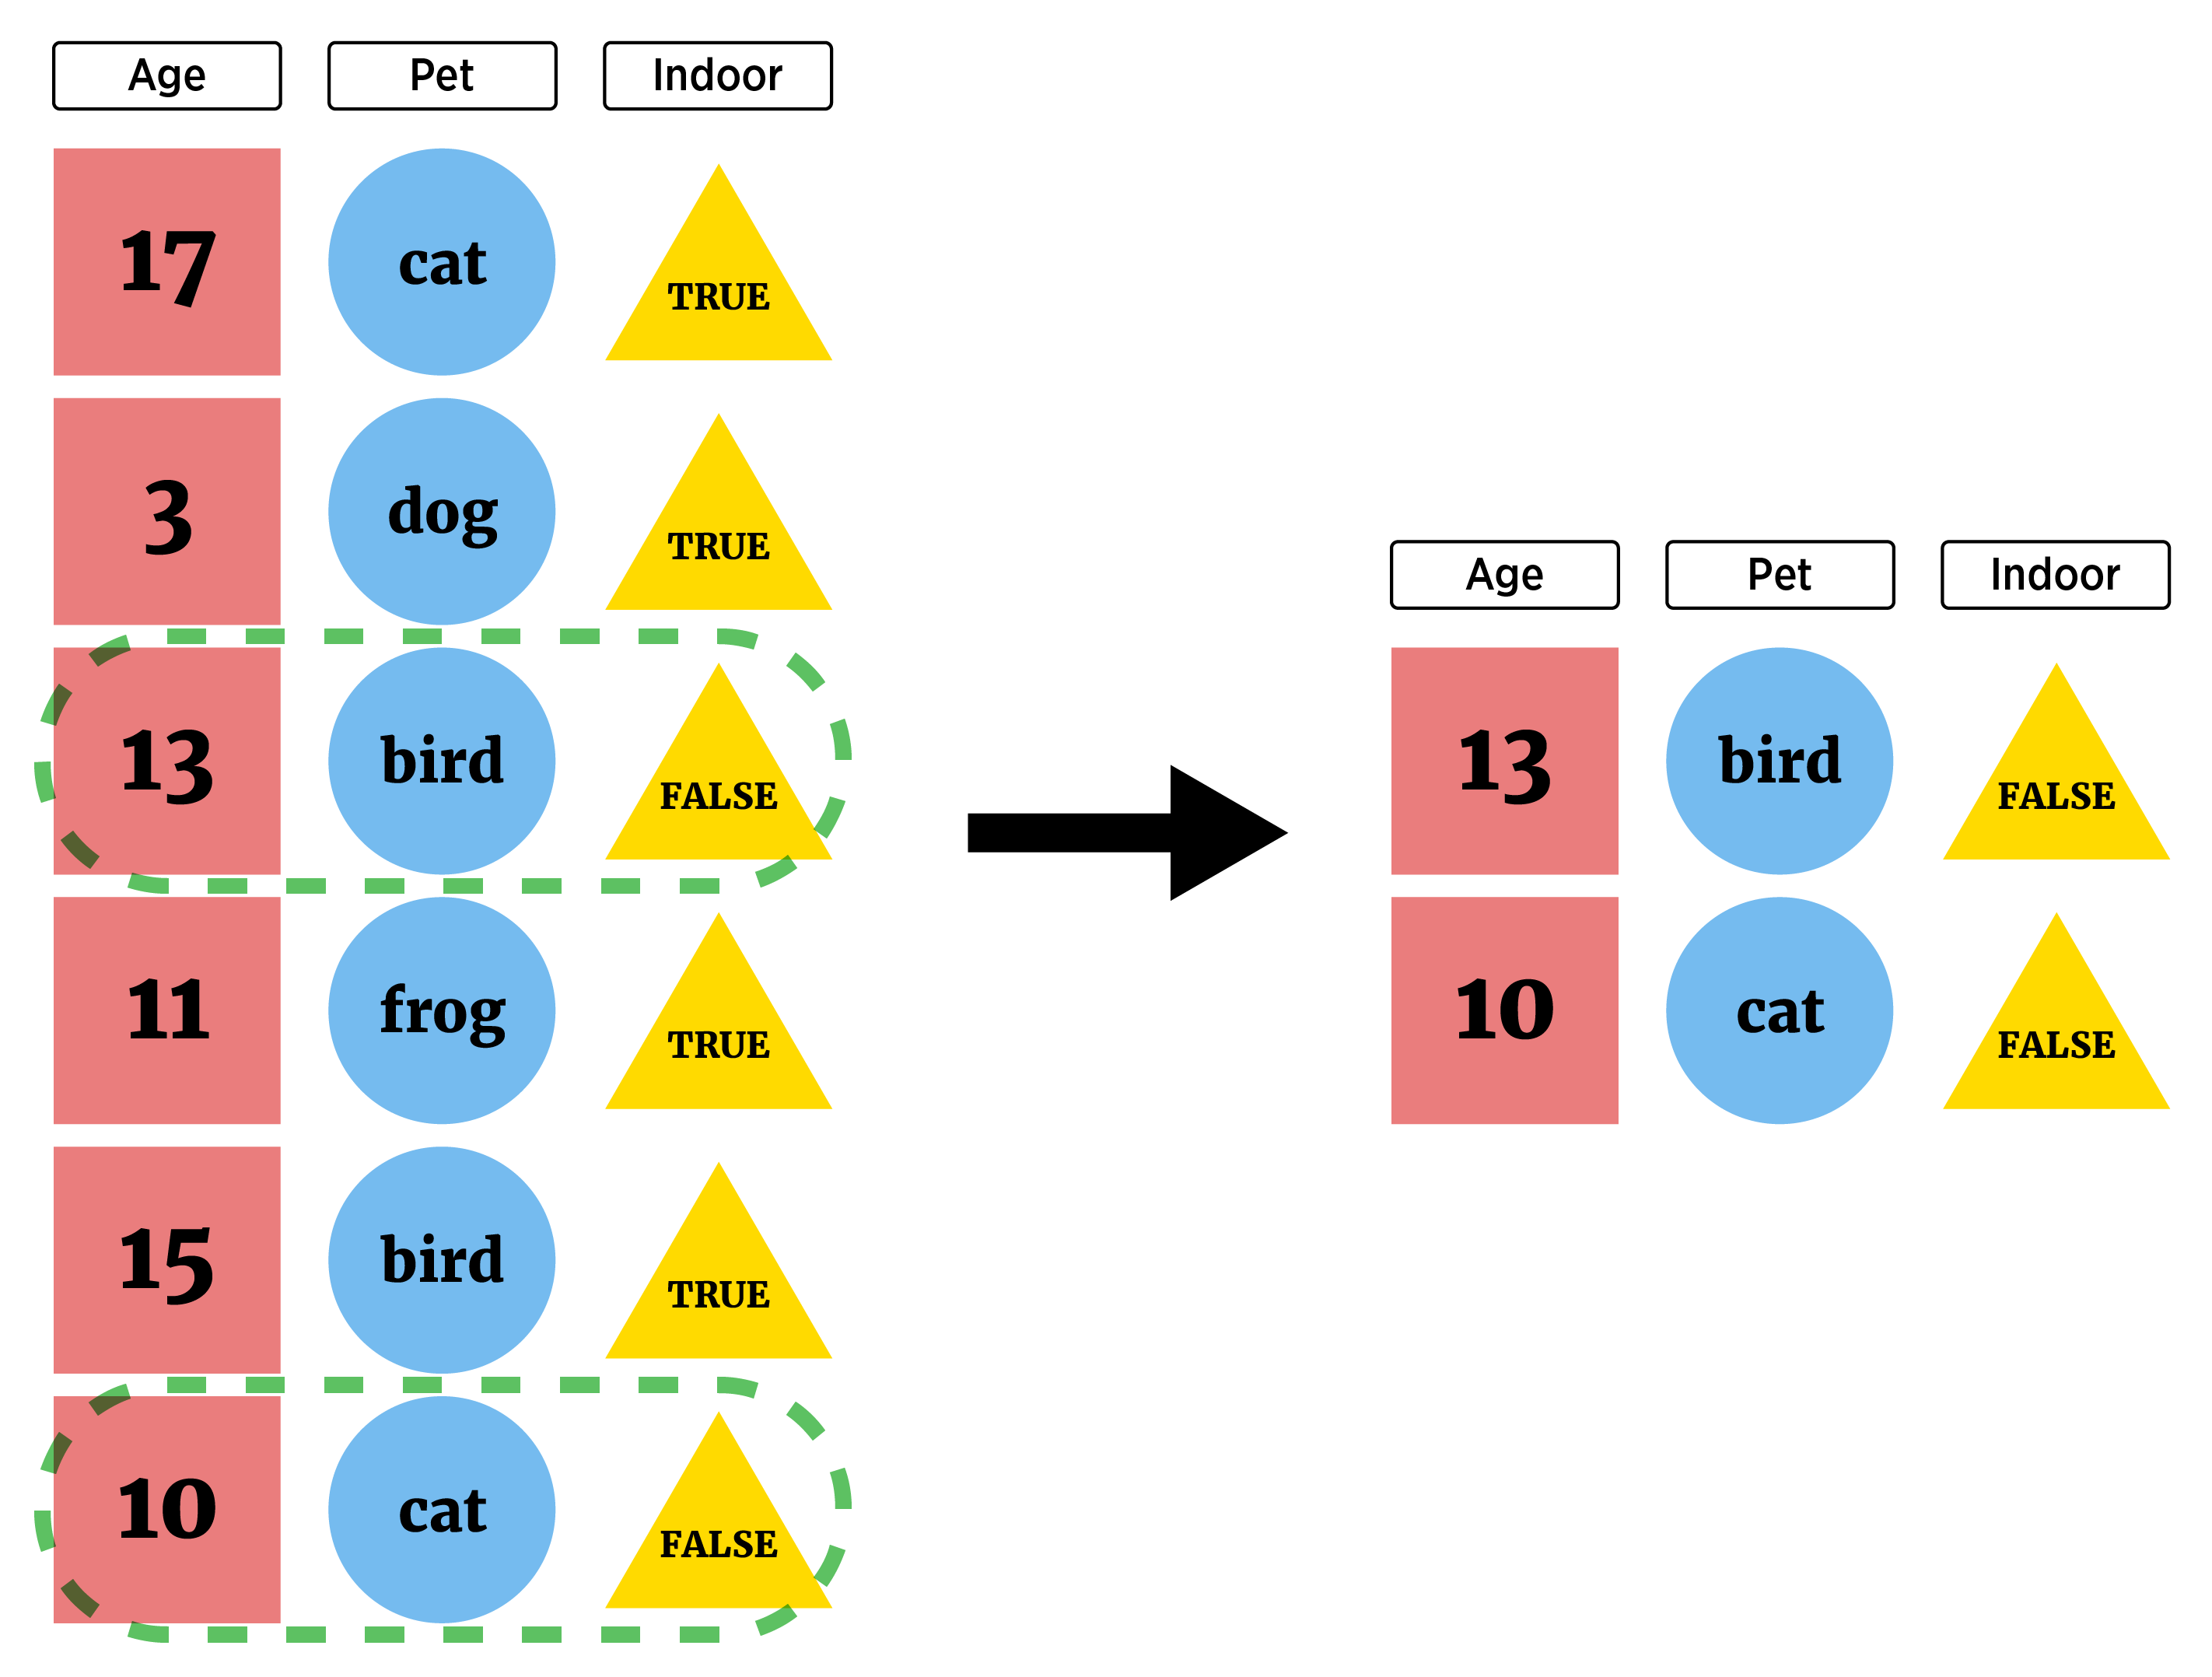
\includegraphics[width=0.8\linewidth]{img/filterVisualF} \end{center}

We just looked at using the \texttt{filter} function to subset rows or observations of a dataset. Let's look at a few more examples. We may only want to return observations from the Batting dataset corresponding to the Pittsburgh Pirates (PIT).

\begin{Shaded}
\begin{Highlighting}[]
\KeywordTok{filter}\NormalTok{(Batting, teamID }\OperatorTok{==}\StringTok{ "PIT"}\NormalTok{)}
\end{Highlighting}
\end{Shaded}

\begin{verbatim}
## # A tibble: 4,817 x 22
##   playerID yearID stint teamID lgID      G    AB     R     H   X2B   X3B    HR
##   <chr>     <int> <int> <fct>  <fct> <int> <int> <int> <int> <int> <int> <int>
## 1 barklsa~   1887     1 PIT    NL       89   340    44    76    10     4     1
## 2 beeched~   1887     1 PIT    NL       41   169    15    41     8     0     2
## 3 bishobi~   1887     1 PIT    NL        3     9     0     0     0     0     0
## 4 brownto~   1887     1 PIT    NL       47   192    30    47     3     4     0
## 5 carrofr~   1887     1 PIT    NL      102   421    71   138    24    15     6
## # ... with 4,812 more rows, and 10 more variables: RBI <int>, SB <int>,
## #   CS <int>, BB <int>, SO <int>, IBB <int>, HBP <int>, SH <int>, SF <int>,
## #   GIDP <int>
\end{verbatim}

We could use a compound logical to only return Pirate data from the year 2000.

\begin{Shaded}
\begin{Highlighting}[]
\KeywordTok{filter}\NormalTok{(Batting, teamID }\OperatorTok{==}\StringTok{ "PIT"} \OperatorTok{&}\StringTok{ }\NormalTok{yearID }\OperatorTok{==}\StringTok{ }\DecValTok{2000}\NormalTok{)}
\end{Highlighting}
\end{Shaded}

\begin{verbatim}
## # A tibble: 46 x 22
##   playerID yearID stint teamID lgID      G    AB     R     H   X2B   X3B    HR
##   <chr>     <int> <int> <fct>  <fct> <int> <int> <int> <int> <int> <int> <int>
## 1 anderji~   2000     1 PIT    NL       27    50     5     7     1     0     0
## 2 arroybr~   2000     1 PIT    NL       21    21     2     3     2     0     0
## 3 avenbr01   2000     1 PIT    NL       72   148    18    37    11     0     5
## 4 benjami~   2000     1 PIT    NL       93   233    28    63    18     2     2
## 5 bensokr~   2000     1 PIT    NL       32    65     3     6     2     0     0
## # ... with 41 more rows, and 10 more variables: RBI <int>, SB <int>, CS <int>,
## #   BB <int>, SO <int>, IBB <int>, HBP <int>, SH <int>, SF <int>, GIDP <int>
\end{verbatim}

Another useful row operation is to rearrange the data based on some criteria. The \texttt{arrange} function allows us to sort a data set by numeric or character variables. For instance we could reorder alphabetically by the teamID variable.

\begin{Shaded}
\begin{Highlighting}[]
\KeywordTok{arrange}\NormalTok{(Batting, teamID)}
\end{Highlighting}
\end{Shaded}

\begin{verbatim}
## # A tibble: 105,861 x 22
##   playerID yearID stint teamID lgID      G    AB     R     H   X2B   X3B    HR
##   <chr>     <int> <int> <fct>  <fct> <int> <int> <int> <int> <int> <int> <int>
## 1 berrych~   1884     1 ALT    UA        7    25     2     6     0     0     0
## 2 brownji~   1884     1 ALT    UA       21    88    12    22     2     2     1
## 3 carropa~   1884     1 ALT    UA       11    49     4    13     1     0     0
## 4 connojo~   1884     1 ALT    UA        3    11     0     1     0     0     0
## 5 crosscl~   1884     1 ALT    UA        2     7     1     4     1     0     0
## # ... with 1.059e+05 more rows, and 10 more variables: RBI <int>, SB <int>,
## #   CS <int>, BB <int>, SO <int>, IBB <int>, HBP <int>, SH <int>, SF <int>,
## #   GIDP <int>
\end{verbatim}

A secondary arrangement can be done as well (and third, etc.)

\begin{Shaded}
\begin{Highlighting}[]
\KeywordTok{arrange}\NormalTok{(Batting, teamID, G)}
\end{Highlighting}
\end{Shaded}

\begin{verbatim}
## # A tibble: 105,861 x 22
##   playerID yearID stint teamID lgID      G    AB     R     H   X2B   X3B    HR
##   <chr>     <int> <int> <fct>  <fct> <int> <int> <int> <int> <int> <int> <int>
## 1 daisege~   1884     1 ALT    UA        1     4     0     0     0     0     0
## 2 crosscl~   1884     1 ALT    UA        2     7     1     4     1     0     0
## 3 manloch~   1884     1 ALT    UA        2     7     1     3     0     0     0
## 4 connojo~   1884     1 ALT    UA        3    11     0     1     0     0     0
## 5 shafff01   1884     1 ALT    UA        6    19     1     3     0     0     0
## # ... with 1.059e+05 more rows, and 10 more variables: RBI <int>, SB <int>,
## #   CS <int>, BB <int>, SO <int>, IBB <int>, HBP <int>, SH <int>, SF <int>,
## #   GIDP <int>
\end{verbatim}

The arrangement can be done descending as well by giving the column (variable) with \texttt{desc}.

\begin{Shaded}
\begin{Highlighting}[]
\KeywordTok{arrange}\NormalTok{(Batting, teamID, }\KeywordTok{desc}\NormalTok{(G))}
\end{Highlighting}
\end{Shaded}

\begin{verbatim}
## # A tibble: 105,861 x 22
##   playerID yearID stint teamID lgID      G    AB     R     H   X2B   X3B    HR
##   <chr>     <int> <int> <fct>  <fct> <int> <int> <int> <int> <int> <int> <int>
## 1 smithge~   1884     1 ALT    UA       25   108     9    34     8     1     0
## 2 harrifr~   1884     1 ALT    UA       24    95    10    25     2     1     0
## 3 doughch~   1884     1 ALT    UA       23    85     6    22     5     0     0
## 4 murphjo~   1884     1 ALT    UA       23    94    10    14     1     0     0
## 5 brownji~   1884     1 ALT    UA       21    88    12    22     2     2     1
## # ... with 1.059e+05 more rows, and 10 more variables: RBI <int>, SB <int>,
## #   CS <int>, BB <int>, SO <int>, IBB <int>, HBP <int>, SH <int>, SF <int>,
## #   GIDP <int>
\end{verbatim}

\hypertarget{column-manipulations}{%
\subsubsection{Column Manipulations}\label{column-manipulations}}

We may want to look at only certain variables (select columns).

\begin{center}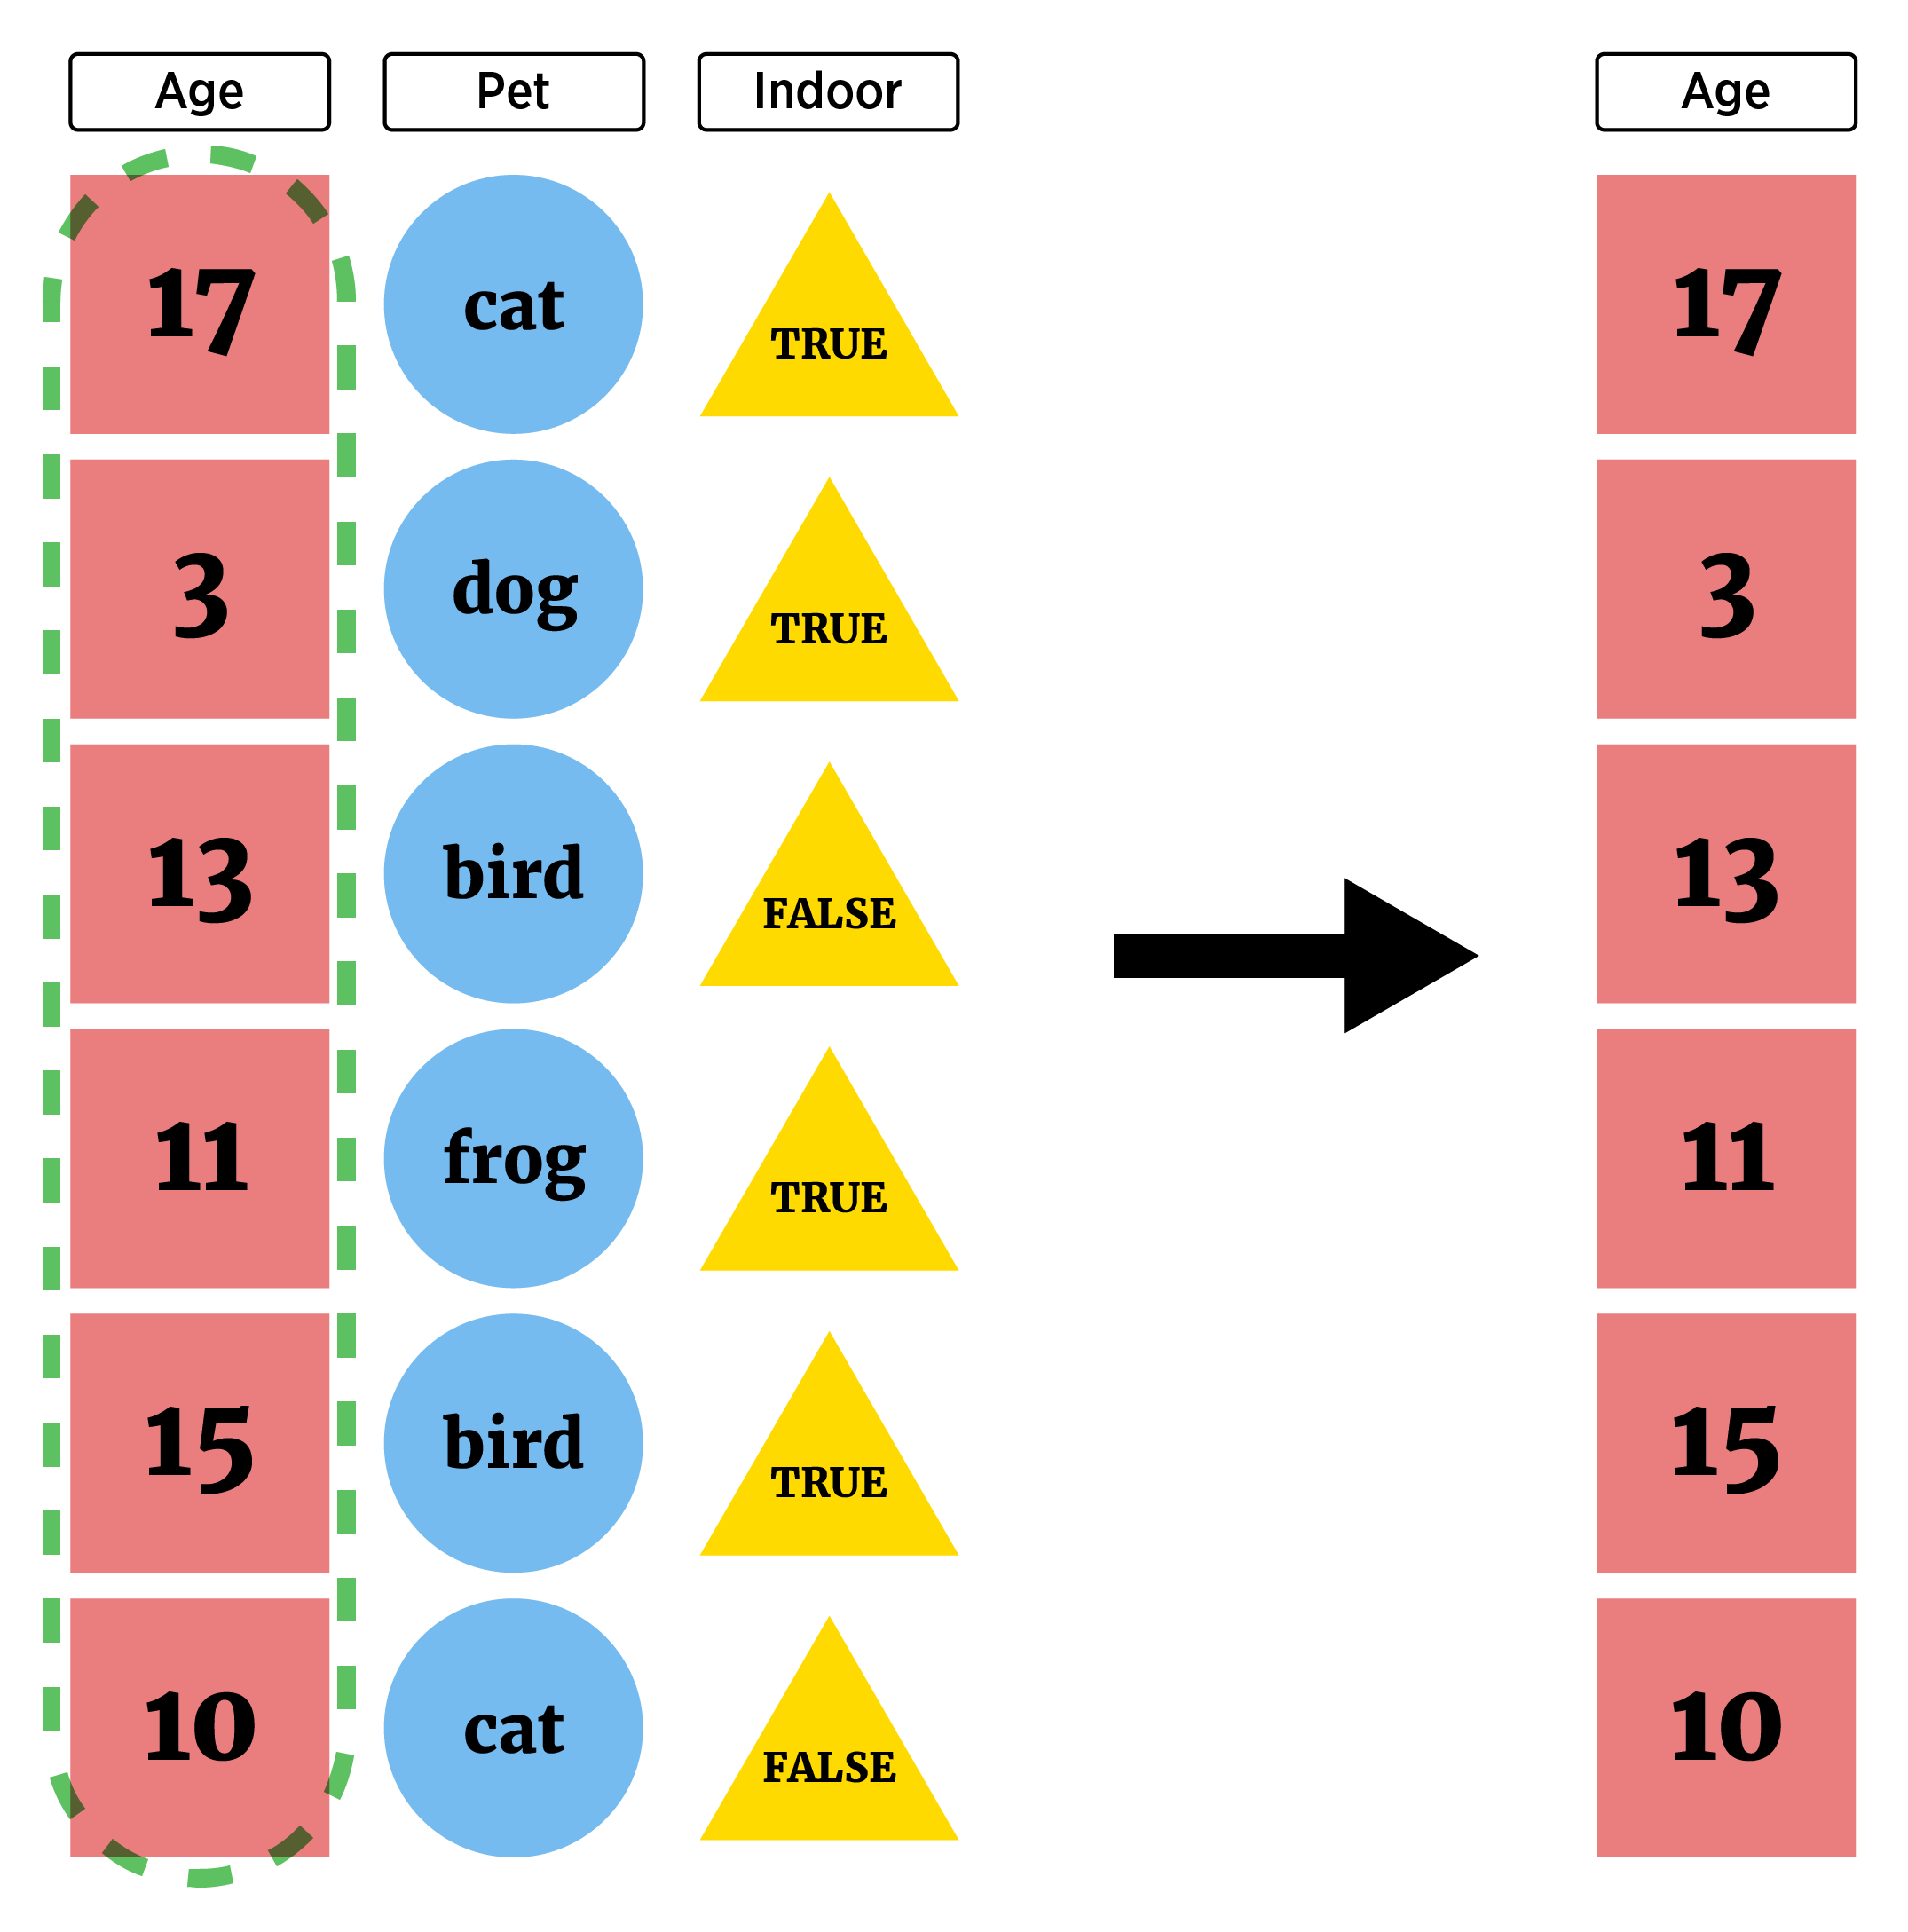
\includegraphics[width=0.65\linewidth]{img/selectVisualF} \end{center}

The \texttt{select} function from the \texttt{dplyr} package allows us to choose columns of interest. We've seen the use of \texttt{\$} and \texttt{{[}\ ,\ {]}} to do this already but \texttt{select} offers many advantages.

\begin{itemize}
\item
  Same syntax as tidyverse functions
\item
  Useful ways to use character matching to select columns
\end{itemize}

Let's see it in action! To choose a single column of interest just supply the column name (or position) after the \texttt{tibble}.

\begin{Shaded}
\begin{Highlighting}[]
\KeywordTok{select}\NormalTok{(Batting, X2B)}
\end{Highlighting}
\end{Shaded}

\begin{verbatim}
## # A tibble: 105,861 x 1
##     X2B
##   <int>
## 1     0
## 2     6
## 3     4
## 4    10
## 5    11
## # ... with 1.059e+05 more rows
\end{verbatim}

Multiple columns can be selected by giving multiple column names.

\begin{Shaded}
\begin{Highlighting}[]
\KeywordTok{select}\NormalTok{(Batting, playerID, X2B)}
\end{Highlighting}
\end{Shaded}

\begin{verbatim}
## # A tibble: 105,861 x 2
##   playerID    X2B
##   <chr>     <int>
## 1 abercda01     0
## 2 addybo01      6
## 3 allisar01     4
## 4 allisdo01    10
## 5 ansonca01    11
## # ... with 1.059e+05 more rows
\end{verbatim}

There are many ways to select multiple columsn (variables). For instance, contiguous columns can be selected using the \texttt{:}.

\begin{Shaded}
\begin{Highlighting}[]
\CommentTok{#all columns between}
\KeywordTok{select}\NormalTok{(Batting, X2B}\OperatorTok{:}\NormalTok{HR)}
\end{Highlighting}
\end{Shaded}

\begin{verbatim}
## # A tibble: 105,861 x 3
##     X2B   X3B    HR
##   <int> <int> <int>
## 1     0     0     0
## 2     6     0     0
## 3     4     5     0
## 4    10     2     2
## 5    11     3     0
## # ... with 1.059e+05 more rows
\end{verbatim}

Character matching can be done to select all columns that contain a certain character.

\begin{Shaded}
\begin{Highlighting}[]
\CommentTok{#all columns containing}
\KeywordTok{select}\NormalTok{(Batting, }\KeywordTok{contains}\NormalTok{(}\StringTok{"X"}\NormalTok{))}
\end{Highlighting}
\end{Shaded}

\begin{verbatim}
## # A tibble: 105,861 x 2
##     X2B   X3B
##   <int> <int>
## 1     0     0
## 2     6     0
## 3     4     5
## 4    10     2
## 5    11     3
## # ... with 1.059e+05 more rows
\end{verbatim}

Similary, there is a \texttt{starts\_with} and \texttt{ends\_with} function.

\begin{Shaded}
\begin{Highlighting}[]
\CommentTok{#all columns starting with}
\KeywordTok{select}\NormalTok{(Batting, }\KeywordTok{starts_with}\NormalTok{(}\StringTok{"X"}\NormalTok{))}
\end{Highlighting}
\end{Shaded}

\begin{verbatim}
## # A tibble: 105,861 x 2
##     X2B   X3B
##   <int> <int>
## 1     0     0
## 2     6     0
## 3     4     5
## 4    10     2
## 5    11     3
## # ... with 1.059e+05 more rows
\end{verbatim}

\begin{Shaded}
\begin{Highlighting}[]
\CommentTok{#multiple selections}
\KeywordTok{select}\NormalTok{(Batting, }\KeywordTok{starts_with}\NormalTok{(}\StringTok{"X"}\NormalTok{), }\KeywordTok{ends_with}\NormalTok{(}\StringTok{"ID"}\NormalTok{), G)}
\end{Highlighting}
\end{Shaded}

\begin{verbatim}
## # A tibble: 105,861 x 7
##     X2B   X3B playerID  yearID teamID lgID      G
##   <int> <int> <chr>      <int> <fct>  <fct> <int>
## 1     0     0 abercda01   1871 TRO    NA        1
## 2     6     0 addybo01    1871 RC1    NA       25
## 3     4     5 allisar01   1871 CL1    NA       29
## 4    10     2 allisdo01   1871 WS3    NA       27
## 5    11     3 ansonca01   1871 RC1    NA       25
## # ... with 1.059e+05 more rows
\end{verbatim}

Sometimes we want to rename variables. This can be done with the \texttt{rename} function.

\begin{Shaded}
\begin{Highlighting}[]
\CommentTok{#rename our previous selection}
\KeywordTok{rename}\NormalTok{(}\KeywordTok{select}\NormalTok{(Batting, }\KeywordTok{starts_with}\NormalTok{(}\StringTok{"X"}\NormalTok{), }\KeywordTok{ends_with}\NormalTok{(}\StringTok{"ID"}\NormalTok{), G), }\StringTok{"Doubles"}\NormalTok{ =}\StringTok{ }\NormalTok{X2B, }\StringTok{"Triples"}\NormalTok{ =}\StringTok{ }\NormalTok{X3B)}
\end{Highlighting}
\end{Shaded}

\begin{verbatim}
## # A tibble: 105,861 x 7
##   Doubles Triples playerID  yearID teamID lgID      G
##     <int>   <int> <chr>      <int> <fct>  <fct> <int>
## 1       0       0 abercda01   1871 TRO    NA        1
## 2       6       0 addybo01    1871 RC1    NA       25
## 3       4       5 allisar01   1871 CL1    NA       29
## 4      10       2 allisdo01   1871 WS3    NA       27
## 5      11       3 ansonca01   1871 RC1    NA       25
## # ... with 1.059e+05 more rows
\end{verbatim}

You may notice this is kind function nesting makes this code difficult for humans to parse. Piping or Chaining can be used to make the use of multiple functions easier!

\texttt{\%\textgreater{}\%} is the piping operator. Generically, piping does the following

\texttt{x\ \%\textgreater{}\%\ f(y)} turns into \texttt{f(x,y)}

\texttt{x\ \%\textgreater{}\%\ f(y)\ \%\textgreater{}\%\ g(z)} turns into \texttt{g(f(x,\ y),\ z)}

Since the tidyverse functions all have the same syntax, piping works wonders for readability! Piping can be used with functions outside the tidyverse if this structure works. Let's rewrite our previous nested function with piping. When reading code with piping, read \texttt{\%\textgreater{}\%} as the word `then.'

Batting data set (then) select these columns (then) rename the variables.

\begin{Shaded}
\begin{Highlighting}[]
\NormalTok{Batting }\OperatorTok\StringTok{ }\KeywordTok{select}\NormalTok{(}\KeywordTok{starts_with}\NormalTok{(}\StringTok{"X"}\NormalTok{), }\KeywordTok{ends_with}\NormalTok{(}\StringTok{"ID"}\NormalTok{), G) }\OperatorTok\StringTok{ }\KeywordTok{rename}\NormalTok{(}\StringTok{"Doubles"}\NormalTok{ =}\StringTok{ }\NormalTok{X2B, }\StringTok{"Triples"}\NormalTok{ =}\StringTok{ }\NormalTok{X3B)}
\end{Highlighting}
\end{Shaded}

\begin{verbatim}
## # A tibble: 105,861 x 7
##   Doubles Triples playerID  yearID teamID lgID      G
##     <int>   <int> <chr>      <int> <fct>  <fct> <int>
## 1       0       0 abercda01   1871 TRO    NA        1
## 2       6       0 addybo01    1871 RC1    NA       25
## 3       4       5 allisar01   1871 CL1    NA       29
## 4      10       2 allisdo01   1871 WS3    NA       27
## 5      11       3 ansonca01   1871 RC1    NA       25
## # ... with 1.059e+05 more rows
\end{verbatim}

We may also wish to reorder our columns (variables). This can be done using \texttt{select}. The \texttt{everything} function is handy so you don't have to list all the variables out if you only want to reorder a few.

\begin{Shaded}
\begin{Highlighting}[]
\NormalTok{Batting }\OperatorTok\StringTok{ }\KeywordTok{select}\NormalTok{(playerID, HR, }\KeywordTok{everything}\NormalTok{())}
\end{Highlighting}
\end{Shaded}

\begin{verbatim}
## # A tibble: 105,861 x 22
##   playerID    HR yearID stint teamID lgID      G    AB     R     H   X2B   X3B
##   <chr>    <int>  <int> <int> <fct>  <fct> <int> <int> <int> <int> <int> <int>
## 1 abercda~     0   1871     1 TRO    NA        1     4     0     0     0     0
## 2 addybo01     0   1871     1 RC1    NA       25   118    30    32     6     0
## 3 allisar~     0   1871     1 CL1    NA       29   137    28    40     4     5
## 4 allisdo~     2   1871     1 WS3    NA       27   133    28    44    10     2
## 5 ansonca~     0   1871     1 RC1    NA       25   120    29    39    11     3
## # ... with 1.059e+05 more rows, and 10 more variables: RBI <int>, SB <int>,
## #   CS <int>, BB <int>, SO <int>, IBB <int>, HBP <int>, SH <int>, SF <int>,
## #   GIDP <int>
\end{verbatim}

Another commonly done column manipulation is the creating of new variables.

\begin{center}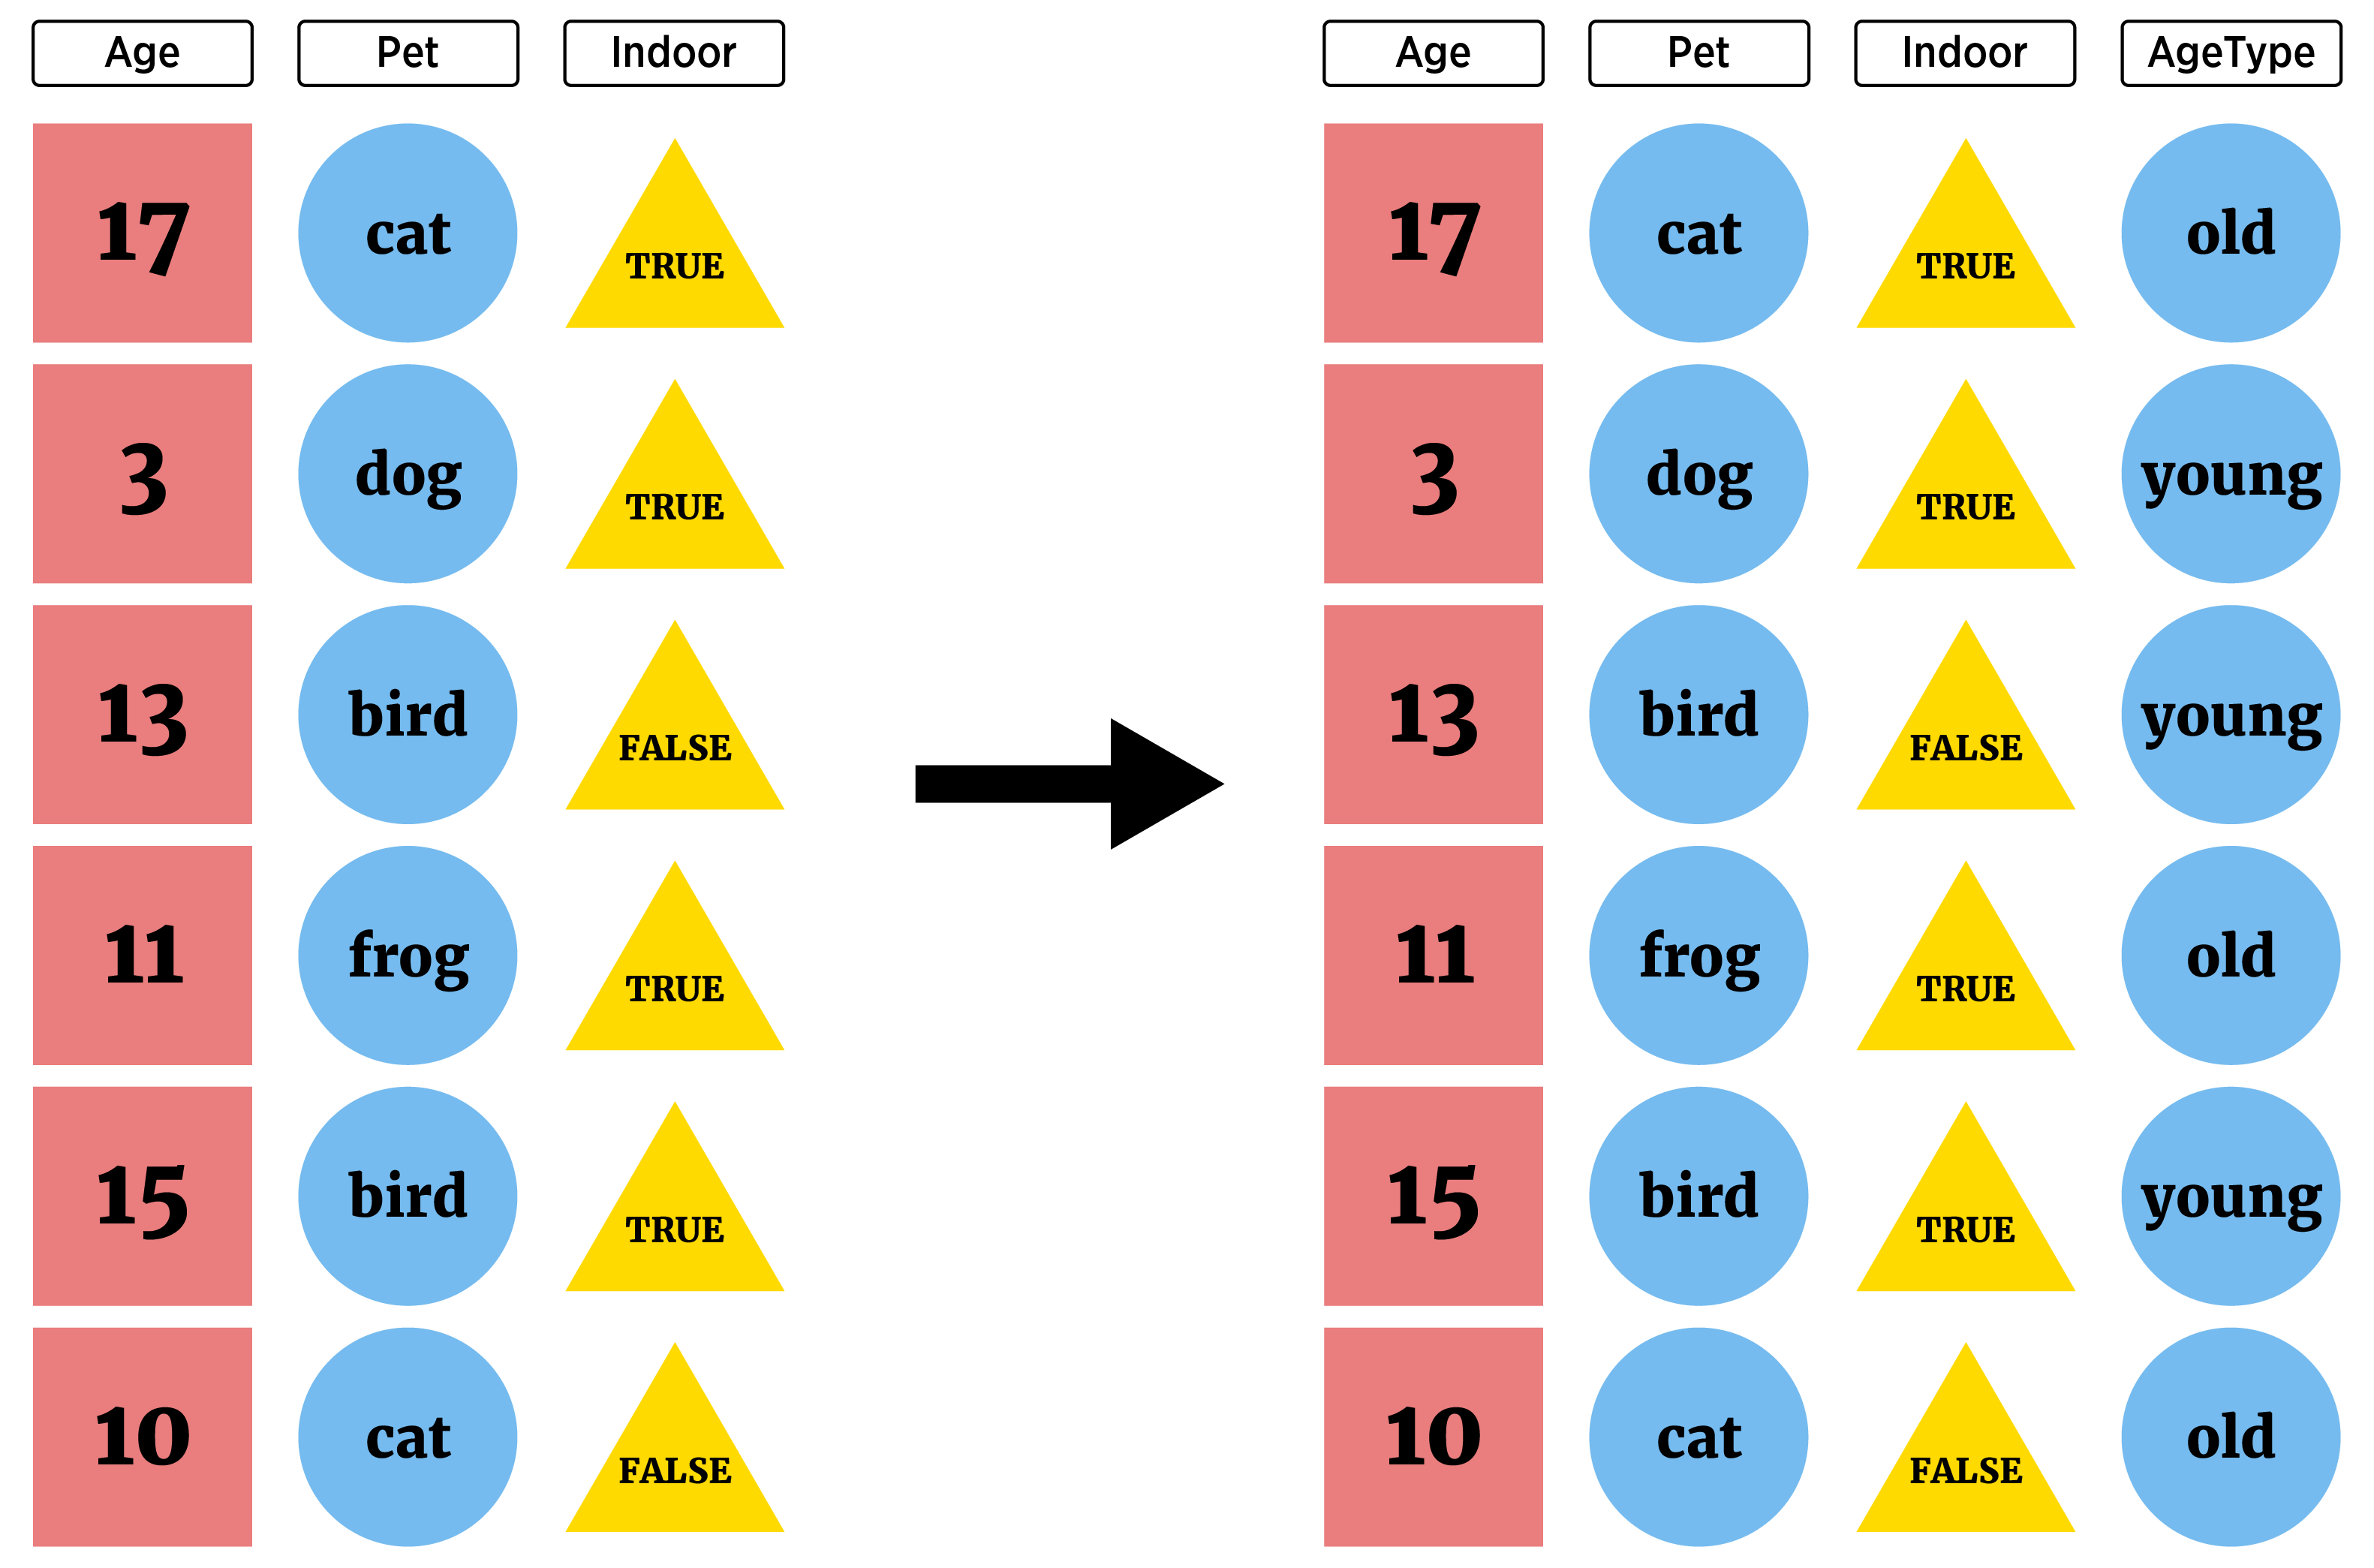
\includegraphics[width=0.8\linewidth]{img/createVarVisualF} \end{center}

Given a data frame and an appropriate length vector (new variable) we can use \texttt{cbind} (column bind) to add the variable to the data frame.

\begin{Shaded}
\begin{Highlighting}[]
\NormalTok{temp <-}\StringTok{ }\KeywordTok{cbind}\NormalTok{(iris, }\DataTypeTok{extra =} \KeywordTok{rep}\NormalTok{(}\StringTok{"a"}\NormalTok{, }\DecValTok{150}\NormalTok{))}
\KeywordTok{str}\NormalTok{(temp)}
\end{Highlighting}
\end{Shaded}

\begin{verbatim}
## 'data.frame':    150 obs. of  6 variables:
##  $ Sepal.Length: num  5.1 4.9 4.7 4.6 5 5.4 4.6 5 4.4 4.9 ...
##  $ Sepal.Width : num  3.5 3 3.2 3.1 3.6 3.9 3.4 3.4 2.9 3.1 ...
##  $ Petal.Length: num  1.4 1.4 1.3 1.5 1.4 1.7 1.4 1.5 1.4 1.5 ...
##  $ Petal.Width : num  0.2 0.2 0.2 0.2 0.2 0.4 0.3 0.2 0.2 0.1 ...
##  $ Species     : Factor w/ 3 levels "setosa","versicolor",..: 1 1 1 1 1 1 1 1 1 1 ...
##  $ extra       : Factor w/ 1 level "a": 1 1 1 1 1 1 1 1 1 1 ...
\end{verbatim}

More simply we can just add the new variable as a named (list) element!

\begin{Shaded}
\begin{Highlighting}[]
\NormalTok{iris}\OperatorTok{$}\NormalTok{extra <-}\StringTok{ }\KeywordTok{rep}\NormalTok{(}\StringTok{"a"}\NormalTok{, }\DecValTok{150}\NormalTok{)}
\KeywordTok{str}\NormalTok{(iris)}
\end{Highlighting}
\end{Shaded}

\begin{verbatim}
## 'data.frame':    150 obs. of  6 variables:
##  $ Sepal.Length: num  5.1 4.9 4.7 4.6 5 5.4 4.6 5 4.4 4.9 ...
##  $ Sepal.Width : num  3.5 3 3.2 3.1 3.6 3.9 3.4 3.4 2.9 3.1 ...
##  $ Petal.Length: num  1.4 1.4 1.3 1.5 1.4 1.7 1.4 1.5 1.4 1.5 ...
##  $ Petal.Width : num  0.2 0.2 0.2 0.2 0.2 0.4 0.3 0.2 0.2 0.1 ...
##  $ Species     : Factor w/ 3 levels "setosa","versicolor",..: 1 1 1 1 1 1 1 1 1 1 ...
##  $ extra       : chr  "a" "a" "a" "a" ...
\end{verbatim}

To stay in the tidyverse and add more functionality we can use two functions from \texttt{dplyr}:

\begin{itemize}
\item
  \texttt{mutate()} - add newly created column(s) to current data frame
\item
  \texttt{transmute()} - create new data frame with created variable(s)
\end{itemize}

The syntax for these functions is similar to previous. We simply name the new variables after specifying our data set.

\texttt{mutate(data,\ newVarName\ =\ functionOfData,\ newVarName2\ =\ functionOfData,\ ...)}\\
For this section let's consider a data set on movie ratings from the \texttt{fivethirtyeight} package.

\begin{Shaded}
\begin{Highlighting}[]
\KeywordTok{library}\NormalTok{(fivethirtyeight)}
\end{Highlighting}
\end{Shaded}

\begin{verbatim}
## Warning: package 'fivethirtyeight' was built under R version 3.6.3
\end{verbatim}

\begin{Shaded}
\begin{Highlighting}[]
\NormalTok{fandango}
\end{Highlighting}
\end{Shaded}

\begin{verbatim}
## # A tibble: 146 x 23
##   film   year rottentomatoes rottentomatoes_~ metacritic metacritic_user  imdb
##   <chr> <dbl>          <int>            <int>      <int>           <dbl> <dbl>
## 1 Aven~  2015             74               86         66             7.1   7.8
## 2 Cind~  2015             85               80         67             7.5   7.1
## 3 Ant-~  2015             80               90         64             8.1   7.8
## 4 Do Y~  2015             18               84         22             4.7   5.4
## 5 Hot ~  2015             14               28         29             3.4   5.1
## # ... with 141 more rows, and 16 more variables: fandango_stars <dbl>,
## #   fandango_ratingvalue <dbl>, rt_norm <dbl>, rt_user_norm <dbl>,
## #   metacritic_norm <dbl>, metacritic_user_nom <dbl>, imdb_norm <dbl>,
## #   rt_norm_round <dbl>, rt_user_norm_round <dbl>, metacritic_norm_round <dbl>,
## #   metacritic_user_norm_round <dbl>, imdb_norm_round <dbl>,
## #   metacritic_user_vote_count <int>, imdb_user_vote_count <int>,
## #   fandango_votes <int>, fandango_difference <dbl>
\end{verbatim}

We can add a new variable that is the average of two columns using \texttt{mutate}. Remember to read \texttt{\%\textgreater{}\%} as `then.'

\begin{Shaded}
\begin{Highlighting}[]
\NormalTok{fandango }\OperatorTok\StringTok{ }\KeywordTok{mutate}\NormalTok{(}\DataTypeTok{avgRotten =}\NormalTok{ (rottentomatoes }\OperatorTok{+}\StringTok{ }\NormalTok{rottentomatoes_user)}\OperatorTok{/}\DecValTok{2}\NormalTok{) }\OperatorTok\StringTok{ }
\StringTok{  }\KeywordTok{select}\NormalTok{(film, year, avgRotten, }\KeywordTok{everything}\NormalTok{())}
\end{Highlighting}
\end{Shaded}

\begin{verbatim}
## # A tibble: 146 x 24
##   film   year avgRotten rottentomatoes rottentomatoes_~ metacritic
##   <chr> <dbl>     <dbl>          <int>            <int>      <int>
## 1 Aven~  2015      80               74               86         66
## 2 Cind~  2015      82.5             85               80         67
## 3 Ant-~  2015      85               80               90         64
## 4 Do Y~  2015      51               18               84         22
## 5 Hot ~  2015      21               14               28         29
## # ... with 141 more rows, and 18 more variables: metacritic_user <dbl>,
## #   imdb <dbl>, fandango_stars <dbl>, fandango_ratingvalue <dbl>,
## #   rt_norm <dbl>, rt_user_norm <dbl>, metacritic_norm <dbl>,
## #   metacritic_user_nom <dbl>, imdb_norm <dbl>, rt_norm_round <dbl>,
## #   rt_user_norm_round <dbl>, metacritic_norm_round <dbl>,
## #   metacritic_user_norm_round <dbl>, imdb_norm_round <dbl>,
## #   metacritic_user_vote_count <int>, imdb_user_vote_count <int>,
## #   fandango_votes <int>, fandango_difference <dbl>
\end{verbatim}

More than one variable can be created. Here an average of the normed metacritic scores.

\begin{Shaded}
\begin{Highlighting}[]
\NormalTok{fandango }\OperatorTok\StringTok{ }
\StringTok{  }\KeywordTok{mutate}\NormalTok{(}\DataTypeTok{avgRotten =}\NormalTok{ (rottentomatoes }\OperatorTok{+}\StringTok{ }\NormalTok{rottentomatoes_user)}\OperatorTok{/}\DecValTok{2}\NormalTok{, }
         \DataTypeTok{avgMeta =}\NormalTok{ (metacritic_norm }\OperatorTok{+}\StringTok{ }\NormalTok{metacritic_user_nom)}\OperatorTok{/}\DecValTok{2}\NormalTok{) }\OperatorTok
\StringTok{  }\KeywordTok{select}\NormalTok{(film, year, avgRotten, avgMeta, }\KeywordTok{everything}\NormalTok{())}
\end{Highlighting}
\end{Shaded}

\begin{verbatim}
## # A tibble: 146 x 25
##   film   year avgRotten avgMeta rottentomatoes rottentomatoes_~ metacritic
##   <chr> <dbl>     <dbl>   <dbl>          <int>            <int>      <int>
## 1 Aven~  2015      80      3.42             74               86         66
## 2 Cind~  2015      82.5    3.55             85               80         67
## 3 Ant-~  2015      85      3.62             80               90         64
## 4 Do Y~  2015      51      1.72             18               84         22
## 5 Hot ~  2015      21      1.58             14               28         29
## # ... with 141 more rows, and 18 more variables: metacritic_user <dbl>,
## #   imdb <dbl>, fandango_stars <dbl>, fandango_ratingvalue <dbl>,
## #   rt_norm <dbl>, rt_user_norm <dbl>, metacritic_norm <dbl>,
## #   metacritic_user_nom <dbl>, imdb_norm <dbl>, rt_norm_round <dbl>,
## #   rt_user_norm_round <dbl>, metacritic_norm_round <dbl>,
## #   metacritic_user_norm_round <dbl>, imdb_norm_round <dbl>,
## #   metacritic_user_vote_count <int>, imdb_user_vote_count <int>,
## #   fandango_votes <int>, fandango_difference <dbl>
\end{verbatim}

\texttt{transmute} is very similar to mutate except it doesn't return the original tibble, just the newly created variable(s).

\begin{Shaded}
\begin{Highlighting}[]
\NormalTok{fandango }\OperatorTok\StringTok{ }\KeywordTok{transmute}\NormalTok{(}\DataTypeTok{avgRotten =}\NormalTok{ (rottentomatoes }\OperatorTok{+}\StringTok{ }\NormalTok{rottentomatoes_user)}\OperatorTok{/}\DecValTok{2}\NormalTok{)}
\end{Highlighting}
\end{Shaded}

\begin{verbatim}
## # A tibble: 146 x 1
##   avgRotten
##       <dbl>
## 1      80  
## 2      82.5
## 3      85  
## 4      51  
## 5      21  
## # ... with 141 more rows
\end{verbatim}

\begin{Shaded}
\begin{Highlighting}[]
\NormalTok{fandango }\OperatorTok\StringTok{ }\KeywordTok{transmute}\NormalTok{(}\DataTypeTok{avgRotten =}\NormalTok{ (rottentomatoes }\OperatorTok{+}\StringTok{ }\NormalTok{rottentomatoes_user)}\OperatorTok{/}\DecValTok{2}\NormalTok{, }
                       \DataTypeTok{avgMeta =}\NormalTok{ (metacritic_norm }\OperatorTok{+}\StringTok{ }\NormalTok{metacritic_user_nom)}\OperatorTok{/}\DecValTok{2}\NormalTok{) }
\end{Highlighting}
\end{Shaded}

\begin{verbatim}
## # A tibble: 146 x 2
##   avgRotten avgMeta
##       <dbl>   <dbl>
## 1      80      3.42
## 2      82.5    3.55
## 3      85      3.62
## 4      51      1.72
## 5      21      1.58
## # ... with 141 more rows
\end{verbatim}

\texttt{mutate} and \texttt{transmute} can also use `window' functions. These are functions that take a vector of values and return another vector of values (see \href{https://www.rstudio.com/wp-content/uploads/2015/02/data-wrangling-cheatsheet.pdf}{Cheat sheet}). For instance we can find the cumulative sum of a column using \texttt{cumsum}.

\begin{Shaded}
\begin{Highlighting}[]
\NormalTok{fandango }\OperatorTok\StringTok{ }\KeywordTok{select}\NormalTok{(rottentomatoes) }\OperatorTok\StringTok{ }\KeywordTok{mutate}\NormalTok{(}\DataTypeTok{cumulativeSum =} \KeywordTok{cumsum}\NormalTok{(rottentomatoes))}
\end{Highlighting}
\end{Shaded}

\begin{verbatim}
## # A tibble: 146 x 2
##   rottentomatoes cumulativeSum
##            <int>         <int>
## 1             74            74
## 2             85           159
## 3             80           239
## 4             18           257
## 5             14           271
## # ... with 141 more rows
\end{verbatim}

\texttt{mutate} and \texttt{transmute} can also use some statistical functions to create new variables. Here we add a column representing the mean and standard deviation of the rottentomatoes score.

\begin{Shaded}
\begin{Highlighting}[]
\NormalTok{fandango }\OperatorTok\StringTok{ }\KeywordTok{select}\NormalTok{(rottentomatoes) }\OperatorTok\StringTok{ }
\StringTok{  }\KeywordTok{mutate}\NormalTok{(}\DataTypeTok{avg =} \KeywordTok{mean}\NormalTok{(rottentomatoes), }\DataTypeTok{sd =} \KeywordTok{sd}\NormalTok{(rottentomatoes))}
\end{Highlighting}
\end{Shaded}

\begin{verbatim}
## # A tibble: 146 x 3
##   rottentomatoes   avg    sd
##            <int> <dbl> <dbl>
## 1             74  60.8  30.2
## 2             85  60.8  30.2
## 3             80  60.8  30.2
## 4             18  60.8  30.2
## 5             14  60.8  30.2
## # ... with 141 more rows
\end{verbatim}

These statistical quantities are easily found for subgroups of the data using the \texttt{group\_by} function. We can group the data set by year and run the same \texttt{mutate} function. Now the mean and standard deviation are found for each year and appended appropriately.

\begin{Shaded}
\begin{Highlighting}[]
\NormalTok{fandango }\OperatorTok\StringTok{ }\KeywordTok{select}\NormalTok{(year, rottentomatoes) }\OperatorTok\StringTok{ }
\StringTok{  }\KeywordTok{group_by}\NormalTok{(year) }\OperatorTok\StringTok{ }\KeywordTok{mutate}\NormalTok{(}\DataTypeTok{avg =} \KeywordTok{mean}\NormalTok{(rottentomatoes), }\DataTypeTok{sd =} \KeywordTok{sd}\NormalTok{(rottentomatoes))}
\end{Highlighting}
\end{Shaded}

\begin{verbatim}
## # A tibble: 146 x 4
## # Groups:   year [2]
##    year rottentomatoes   avg    sd
##   <dbl>          <int> <dbl> <dbl>
## 1  2015             74  58.4  30.3
## 2  2015             85  58.4  30.3
## 3  2015             80  58.4  30.3
## 4  2015             18  58.4  30.3
## 5  2015             14  58.4  30.3
## # ... with 141 more rows
\end{verbatim}

Another important way to create variables is through the use of conditional logic. This allows code to be executed only under certain conditions. The main way this is done is through \texttt{if} \texttt{then} \texttt{else} syntax.

\begin{Shaded}
\begin{Highlighting}[]
\ControlFlowTok{if}\NormalTok{ (condition) \{}
\NormalTok{  then execute code}
\NormalTok{\} }

\CommentTok{#if then else}
\ControlFlowTok{if}\NormalTok{ (condition) \{}
\NormalTok{  execute this code  }
\NormalTok{\} }\ControlFlowTok{else}\NormalTok{ \{}
\NormalTok{  execute this code}
\NormalTok{\}}

\CommentTok{#Or more if statements}
\ControlFlowTok{if}\NormalTok{ (condition) \{}
\NormalTok{  execute this code  }
\NormalTok{\} }\ControlFlowTok{else} \ControlFlowTok{if}\NormalTok{ (condition2) \{}
\NormalTok{  execute this code}
\NormalTok{\} }\ControlFlowTok{else} \ControlFlowTok{if}\NormalTok{ (condition3) \{}
\NormalTok{  execute this code}
\NormalTok{\} }\ControlFlowTok{else}\NormalTok{ \{}
  \CommentTok{#if no conditions met}
\NormalTok{  execute this code}
\NormalTok{\}}
\end{Highlighting}
\end{Shaded}

Consider the built-in data set \texttt{airquality}. This hasdaily air quality measurements in New York from May (Day 1) to September (Day 153) in 1973.

\begin{Shaded}
\begin{Highlighting}[]
\NormalTok{airquality <-}\StringTok{ }\KeywordTok{tbl_df}\NormalTok{(airquality)}
\NormalTok{airquality}
\end{Highlighting}
\end{Shaded}

\begin{verbatim}
## # A tibble: 153 x 6
##   Ozone Solar.R  Wind  Temp Month   Day
##   <int>   <int> <dbl> <int> <int> <int>
## 1    41     190   7.4    67     5     1
## 2    36     118   8      72     5     2
## 3    12     149  12.6    74     5     3
## 4    18     313  11.5    62     5     4
## 5    NA      NA  14.3    56     5     5
## # ... with 148 more rows
\end{verbatim}

We may want to code a wind category variable:

\begin{itemize}
\tightlist
\item
  high wind days (15mph \(\leq\) wind)\\
\item
  windy days (10mph \(\leq\) wind \textless{} 15mph)\\
\item
  lightwind days (6mph \(\leq\) wind \textless{} 10mph)\\
\item
  calm days (wind \(\leq\) 6mph)
\end{itemize}

We may think using of using the standard \texttt{if} statements above. The issue is that \texttt{if(condition)} can only take in a single comparison.

\begin{Shaded}
\begin{Highlighting}[]
\ControlFlowTok{if}\NormalTok{(airquality}\OperatorTok{$}\NormalTok{Wind }\OperatorTok{>=}\StringTok{ }\DecValTok{15}\NormalTok{) \{ }
  \StringTok{"High Wind"}
\NormalTok{  \}}
\end{Highlighting}
\end{Shaded}

\begin{verbatim}
## Warning in if (airquality$Wind >= 15) {: the condition has length > 1 and only
## the first element will be used
\end{verbatim}

If you've programmed before you may think about this as an initial plan:

\begin{itemize}
\item
  loop through each observation
\item
  use if then else to determine wind status
\end{itemize}

There are a number of ways to do looping in R

\begin{itemize}
\item
  \texttt{for}
\item
  \texttt{while}
\item
  \texttt{repeat}
\end{itemize}

The idea of a loop is to run code repeatedly changing something each time. The syntax for the \texttt{for} loop is

\begin{Shaded}
\begin{Highlighting}[]
\ControlFlowTok{for}\NormalTok{(index }\ControlFlowTok{in}\NormalTok{ values)\{}
\NormalTok{  code to be run}
\NormalTok{\}}
\end{Highlighting}
\end{Shaded}

The index defines the `counter' or variable that varies as the loop iterates and `values' define which values the index takes on.

\begin{Shaded}
\begin{Highlighting}[]
\ControlFlowTok{for}\NormalTok{ (i }\ControlFlowTok{in} \DecValTok{1}\OperatorTok{:}\DecValTok{10}\NormalTok{)\{}
  \KeywordTok{print}\NormalTok{(i)}
\NormalTok{\}}
\end{Highlighting}
\end{Shaded}

\begin{verbatim}
## [1] 1
## [1] 2
## [1] 3
## [1] 4
## [1] 5
## [1] 6
## [1] 7
## [1] 8
## [1] 9
## [1] 10
\end{verbatim}

\begin{Shaded}
\begin{Highlighting}[]
\ControlFlowTok{for}\NormalTok{ (index }\ControlFlowTok{in} \KeywordTok{c}\NormalTok{(}\StringTok{"cat"}\NormalTok{,}\StringTok{"hat"}\NormalTok{,}\StringTok{"worm"}\NormalTok{))\{}
  \KeywordTok{print}\NormalTok{(index)}
\NormalTok{\}}
\end{Highlighting}
\end{Shaded}

\begin{verbatim}
## [1] "cat"
## [1] "hat"
## [1] "worm"
\end{verbatim}

If we want to code our wind variable we could run a \texttt{for} loop with \texttt{if} logic inside:

\begin{Shaded}
\begin{Highlighting}[]
\NormalTok{status<-}\KeywordTok{vector}\NormalTok{() }\CommentTok{#initialize vector to save results}

\ControlFlowTok{for}\NormalTok{ (i }\ControlFlowTok{in} \DecValTok{1}\OperatorTok{:}\KeywordTok{nrow}\NormalTok{(airquality))\{}
  \ControlFlowTok{if}\NormalTok{(airquality}\OperatorTok{$}\NormalTok{Wind[i] }\OperatorTok{>=}\StringTok{ }\DecValTok{15}\NormalTok{)\{}
\NormalTok{    status[i] <-}\StringTok{ "HighWind"}
\NormalTok{  \} }\ControlFlowTok{else} \ControlFlowTok{if}\NormalTok{ (airquality}\OperatorTok{$}\NormalTok{Wind[i] }\OperatorTok{>=}\StringTok{ }\DecValTok{10}\NormalTok{)\{}
\NormalTok{    status[i] <-}\StringTok{ "Windy"}
\NormalTok{  \} }\ControlFlowTok{else} \ControlFlowTok{if}\NormalTok{ (airquality}\OperatorTok{$}\NormalTok{Wind[i] }\OperatorTok{>=}\StringTok{ }\DecValTok{6}\NormalTok{)\{}
\NormalTok{    status[i] <-}\StringTok{ "LightWind"}
\NormalTok{  \} }\ControlFlowTok{else} \ControlFlowTok{if}\NormalTok{ (airquality}\OperatorTok{$}\NormalTok{Wind[i] }\OperatorTok{>=}\StringTok{ }\DecValTok{0}\NormalTok{)\{}
\NormalTok{    status[i] <-}\StringTok{ "Calm"}
\NormalTok{  \} }\ControlFlowTok{else}\NormalTok{ \{}
\NormalTok{    status[i] <-}\StringTok{ "Error"}
\NormalTok{  \}}
\NormalTok{\}}
\end{Highlighting}
\end{Shaded}

Then we can append the new variable to our dataset.

\begin{Shaded}
\begin{Highlighting}[]
\NormalTok{airquality}\OperatorTok{$}\NormalTok{status <-}\StringTok{ }\NormalTok{status}
\NormalTok{airquality}\OperatorTok{$}\NormalTok{status}
\end{Highlighting}
\end{Shaded}

\begin{verbatim}
##   [1] "LightWind" "LightWind" "Windy"     "Windy"     "Windy"     "Windy"    
##   [7] "LightWind" "Windy"     "HighWind"  "LightWind" "LightWind" "LightWind"
##  [13] "LightWind" "Windy"     "Windy"     "Windy"     "Windy"     "HighWind" 
##  [19] "Windy"     "LightWind" "LightWind" "HighWind"  "LightWind" "Windy"    
##  [25] "HighWind"  "Windy"     "LightWind" "Windy"     "Windy"     "Calm"     
##  [31] "LightWind" "LightWind" "LightWind" "HighWind"  "LightWind" "LightWind"
##  [37] "Windy"     "LightWind" "LightWind" "Windy"     "Windy"     "Windy"    
##  [43] "LightWind" "LightWind" "Windy"     "Windy"     "Windy"     "HighWind" 
##  [49] "LightWind" "Windy"     "Windy"     "LightWind" "Calm"      "Calm"     
##  [55] "LightWind" "LightWind" "LightWind" "Windy"     "Windy"     "Windy"    
##  [61] "LightWind" "Calm"      "LightWind" "LightWind" "Windy"     "Calm"     
##  [67] "Windy"     "Calm"      "LightWind" "Calm"      "LightWind" "LightWind"
##  [73] "Windy"     "Windy"     "Windy"     "Windy"     "LightWind" "Windy"    
##  [79] "LightWind" "Calm"      "Windy"     "LightWind" "LightWind" "Windy"    
##  [85] "LightWind" "LightWind" "LightWind" "Windy"     "LightWind" "LightWind"
##  [91] "LightWind" "LightWind" "LightWind" "Windy"     "LightWind" "LightWind"
##  [97] "LightWind" "Calm"      "Calm"      "Windy"    
##  [ reached getOption("max.print") -- omitted 53 entries ]
\end{verbatim}

This works just fine! Some other things to be aware of with loops:

\begin{itemize}
\tightlist
\item
  \texttt{break} kicks you out of the loop
\end{itemize}

\begin{Shaded}
\begin{Highlighting}[]
\ControlFlowTok{for}\NormalTok{ (i }\ControlFlowTok{in} \DecValTok{1}\OperatorTok{:}\DecValTok{5}\NormalTok{)\{}
    \ControlFlowTok{if}\NormalTok{ (i }\OperatorTok{==}\StringTok{ }\DecValTok{3}\NormalTok{)\{ }
      \ControlFlowTok{break} 
\NormalTok{      \}}
  \KeywordTok{print}\NormalTok{(i)}
\NormalTok{\}}
\end{Highlighting}
\end{Shaded}

\begin{verbatim}
## [1] 1
## [1] 2
\end{verbatim}

\begin{itemize}
\tightlist
\item
  \texttt{next} jumps to the next iteration of the loop
\end{itemize}

\begin{Shaded}
\begin{Highlighting}[]
\ControlFlowTok{for}\NormalTok{ (i }\ControlFlowTok{in} \DecValTok{1}\OperatorTok{:}\DecValTok{5}\NormalTok{)\{}
    \ControlFlowTok{if}\NormalTok{ (i }\OperatorTok{==}\StringTok{ }\DecValTok{3}\NormalTok{)\{}
      \ControlFlowTok{next}
\NormalTok{    \} }
  \KeywordTok{print}\NormalTok{(i)}
\NormalTok{\}}
\end{Highlighting}
\end{Shaded}

\begin{verbatim}
## [1] 1
## [1] 2
## [1] 4
## [1] 5
\end{verbatim}

\begin{itemize}
\tightlist
\item
  \texttt{while} loop are similar
\end{itemize}

\begin{Shaded}
\begin{Highlighting}[]
\ControlFlowTok{while}\NormalTok{(condition) \{}
\NormalTok{    expression to evaluate}
\NormalTok{  modify condition?}
\NormalTok{\}}
\end{Highlighting}
\end{Shaded}

The main issue with loops in R is that they are inefficient. R is an interpreted language so it must figure out how to evaluate code at each iteration of loop, slowing it down.

Vectorized functions are much faster! These functions work on an entire vector at once so R doesn't have to figure things out as often. \texttt{ifelse()} is a vectorized version of \texttt{if\ then\ else}. The syntax is:

\begin{Shaded}
\begin{Highlighting}[]
\KeywordTok{ifelse}\NormalTok{(vector_condition, if_true_do_this, if_false_do_this)}
\end{Highlighting}
\end{Shaded}

Now to create our Wind status variable we can nest \texttt{ifelse} statements.

\begin{Shaded}
\begin{Highlighting}[]
\KeywordTok{ifelse}\NormalTok{(airquality}\OperatorTok{$}\NormalTok{Wind }\OperatorTok{>=}\StringTok{ }\DecValTok{15}\NormalTok{, }\StringTok{"HighWind"}\NormalTok{,}
          \KeywordTok{ifelse}\NormalTok{(airquality}\OperatorTok{$}\NormalTok{Wind }\OperatorTok{>=}\StringTok{ }\DecValTok{10}\NormalTok{, }\StringTok{"Windy"}\NormalTok{,}
                 \KeywordTok{ifelse}\NormalTok{(airquality}\OperatorTok{$}\NormalTok{Wind }\OperatorTok{>=}\StringTok{ }\DecValTok{6}\NormalTok{, }\StringTok{"LightWind"}\NormalTok{, }\StringTok{"Calm"}\NormalTok{)))}
\end{Highlighting}
\end{Shaded}

\begin{verbatim}
##   [1] "LightWind" "LightWind" "Windy"     "Windy"     "Windy"     "Windy"    
##   [7] "LightWind" "Windy"     "HighWind"  "LightWind" "LightWind" "LightWind"
##  [13] "LightWind" "Windy"     "Windy"     "Windy"     "Windy"     "HighWind" 
##  [19] "Windy"     "LightWind" "LightWind" "HighWind"  "LightWind" "Windy"    
##  [25] "HighWind"  "Windy"     "LightWind" "Windy"     "Windy"     "Calm"     
##  [31] "LightWind" "LightWind" "LightWind" "HighWind"  "LightWind" "LightWind"
##  [37] "Windy"     "LightWind" "LightWind" "Windy"     "Windy"     "Windy"    
##  [43] "LightWind" "LightWind" "Windy"     "Windy"     "Windy"     "HighWind" 
##  [49] "LightWind" "Windy"     "Windy"     "LightWind" "Calm"      "Calm"     
##  [55] "LightWind" "LightWind" "LightWind" "Windy"     "Windy"     "Windy"    
##  [61] "LightWind" "Calm"      "LightWind" "LightWind" "Windy"     "Calm"     
##  [67] "Windy"     "Calm"      "LightWind" "Calm"      "LightWind" "LightWind"
##  [73] "Windy"     "Windy"     "Windy"     "Windy"     "LightWind" "Windy"    
##  [79] "LightWind" "Calm"      "Windy"     "LightWind" "LightWind" "Windy"    
##  [85] "LightWind" "LightWind" "LightWind" "Windy"     "LightWind" "LightWind"
##  [91] "LightWind" "LightWind" "LightWind" "Windy"     "LightWind" "LightWind"
##  [97] "LightWind" "Calm"      "Calm"      "Windy"    
##  [ reached getOption("max.print") -- omitted 53 entries ]
\end{verbatim}

\texttt{ifelse} can also easily be used with \texttt{transmute()} or \texttt{mutate()}!

\begin{Shaded}
\begin{Highlighting}[]
\KeywordTok{mutate}\NormalTok{(airquality, }\DataTypeTok{status =} \KeywordTok{ifelse}\NormalTok{(airquality}\OperatorTok{$}\NormalTok{Wind }\OperatorTok{>=}\StringTok{ }\DecValTok{15}\NormalTok{, }\StringTok{"HighWind"}\NormalTok{,}
                                \KeywordTok{ifelse}\NormalTok{(airquality}\OperatorTok{$}\NormalTok{Wind }\OperatorTok{>=}\StringTok{ }\DecValTok{10}\NormalTok{, }\StringTok{"Windy"}\NormalTok{,}
                                       \KeywordTok{ifelse}\NormalTok{(airquality}\OperatorTok{$}\NormalTok{Wind }\OperatorTok{>=}\StringTok{ }\DecValTok{6}\NormalTok{, }\StringTok{"LightWind"}\NormalTok{, }\StringTok{"Calm"}\NormalTok{)))}
\NormalTok{)}
\end{Highlighting}
\end{Shaded}

\begin{verbatim}
## # A tibble: 153 x 7
##   Ozone Solar.R  Wind  Temp Month   Day status   
##   <int>   <int> <dbl> <int> <int> <int> <chr>    
## 1    41     190   7.4    67     5     1 LightWind
## 2    36     118   8      72     5     2 LightWind
## 3    12     149  12.6    74     5     3 Windy    
## 4    18     313  11.5    62     5     4 Windy    
## 5    NA      NA  14.3    56     5     5 Windy    
## # ... with 148 more rows
\end{verbatim}

Note: the \texttt{cut} function can also be used to categorize a numeric variable pretty easily.

This covers the major uses of \texttt{dplyr} for manipulating rows and columns. \texttt{dplyr} also has great functionality for doing \texttt{joins} similar to SQL. We'll also see how it can be used to create basic numeric summaries using \texttt{group\_by} and \texttt{summarize}. The \href{https://www.rstudio.com/wp-content/uploads/2015/02/data-wrangling-cheatsheet.pdf}{cheat sheet} is a great reference!

Recap of basic commands:

\begin{itemize}
\tightlist
\item
  \texttt{tbl\_df} - convert data frame to one with better printing\\
\item
  \texttt{filter} - subset rows\\
\item
  \texttt{arrange} - reorder rows\\
\item
  \texttt{select} - subset columns\\
\item
  \texttt{rename} - reorder columns\\
\item
  \texttt{mutate/transmute} - create new variable
\end{itemize}

\hypertarget{reshaping-data}{%
\subsection{Reshaping Data}\label{reshaping-data}}

We've talked about rows being observations and columns being variables. This is generally how most statistical analysis software likes their data to be formatted. This is called `long' format data - each row is an observation. Sometimes data doesn't come that way!

\begin{center}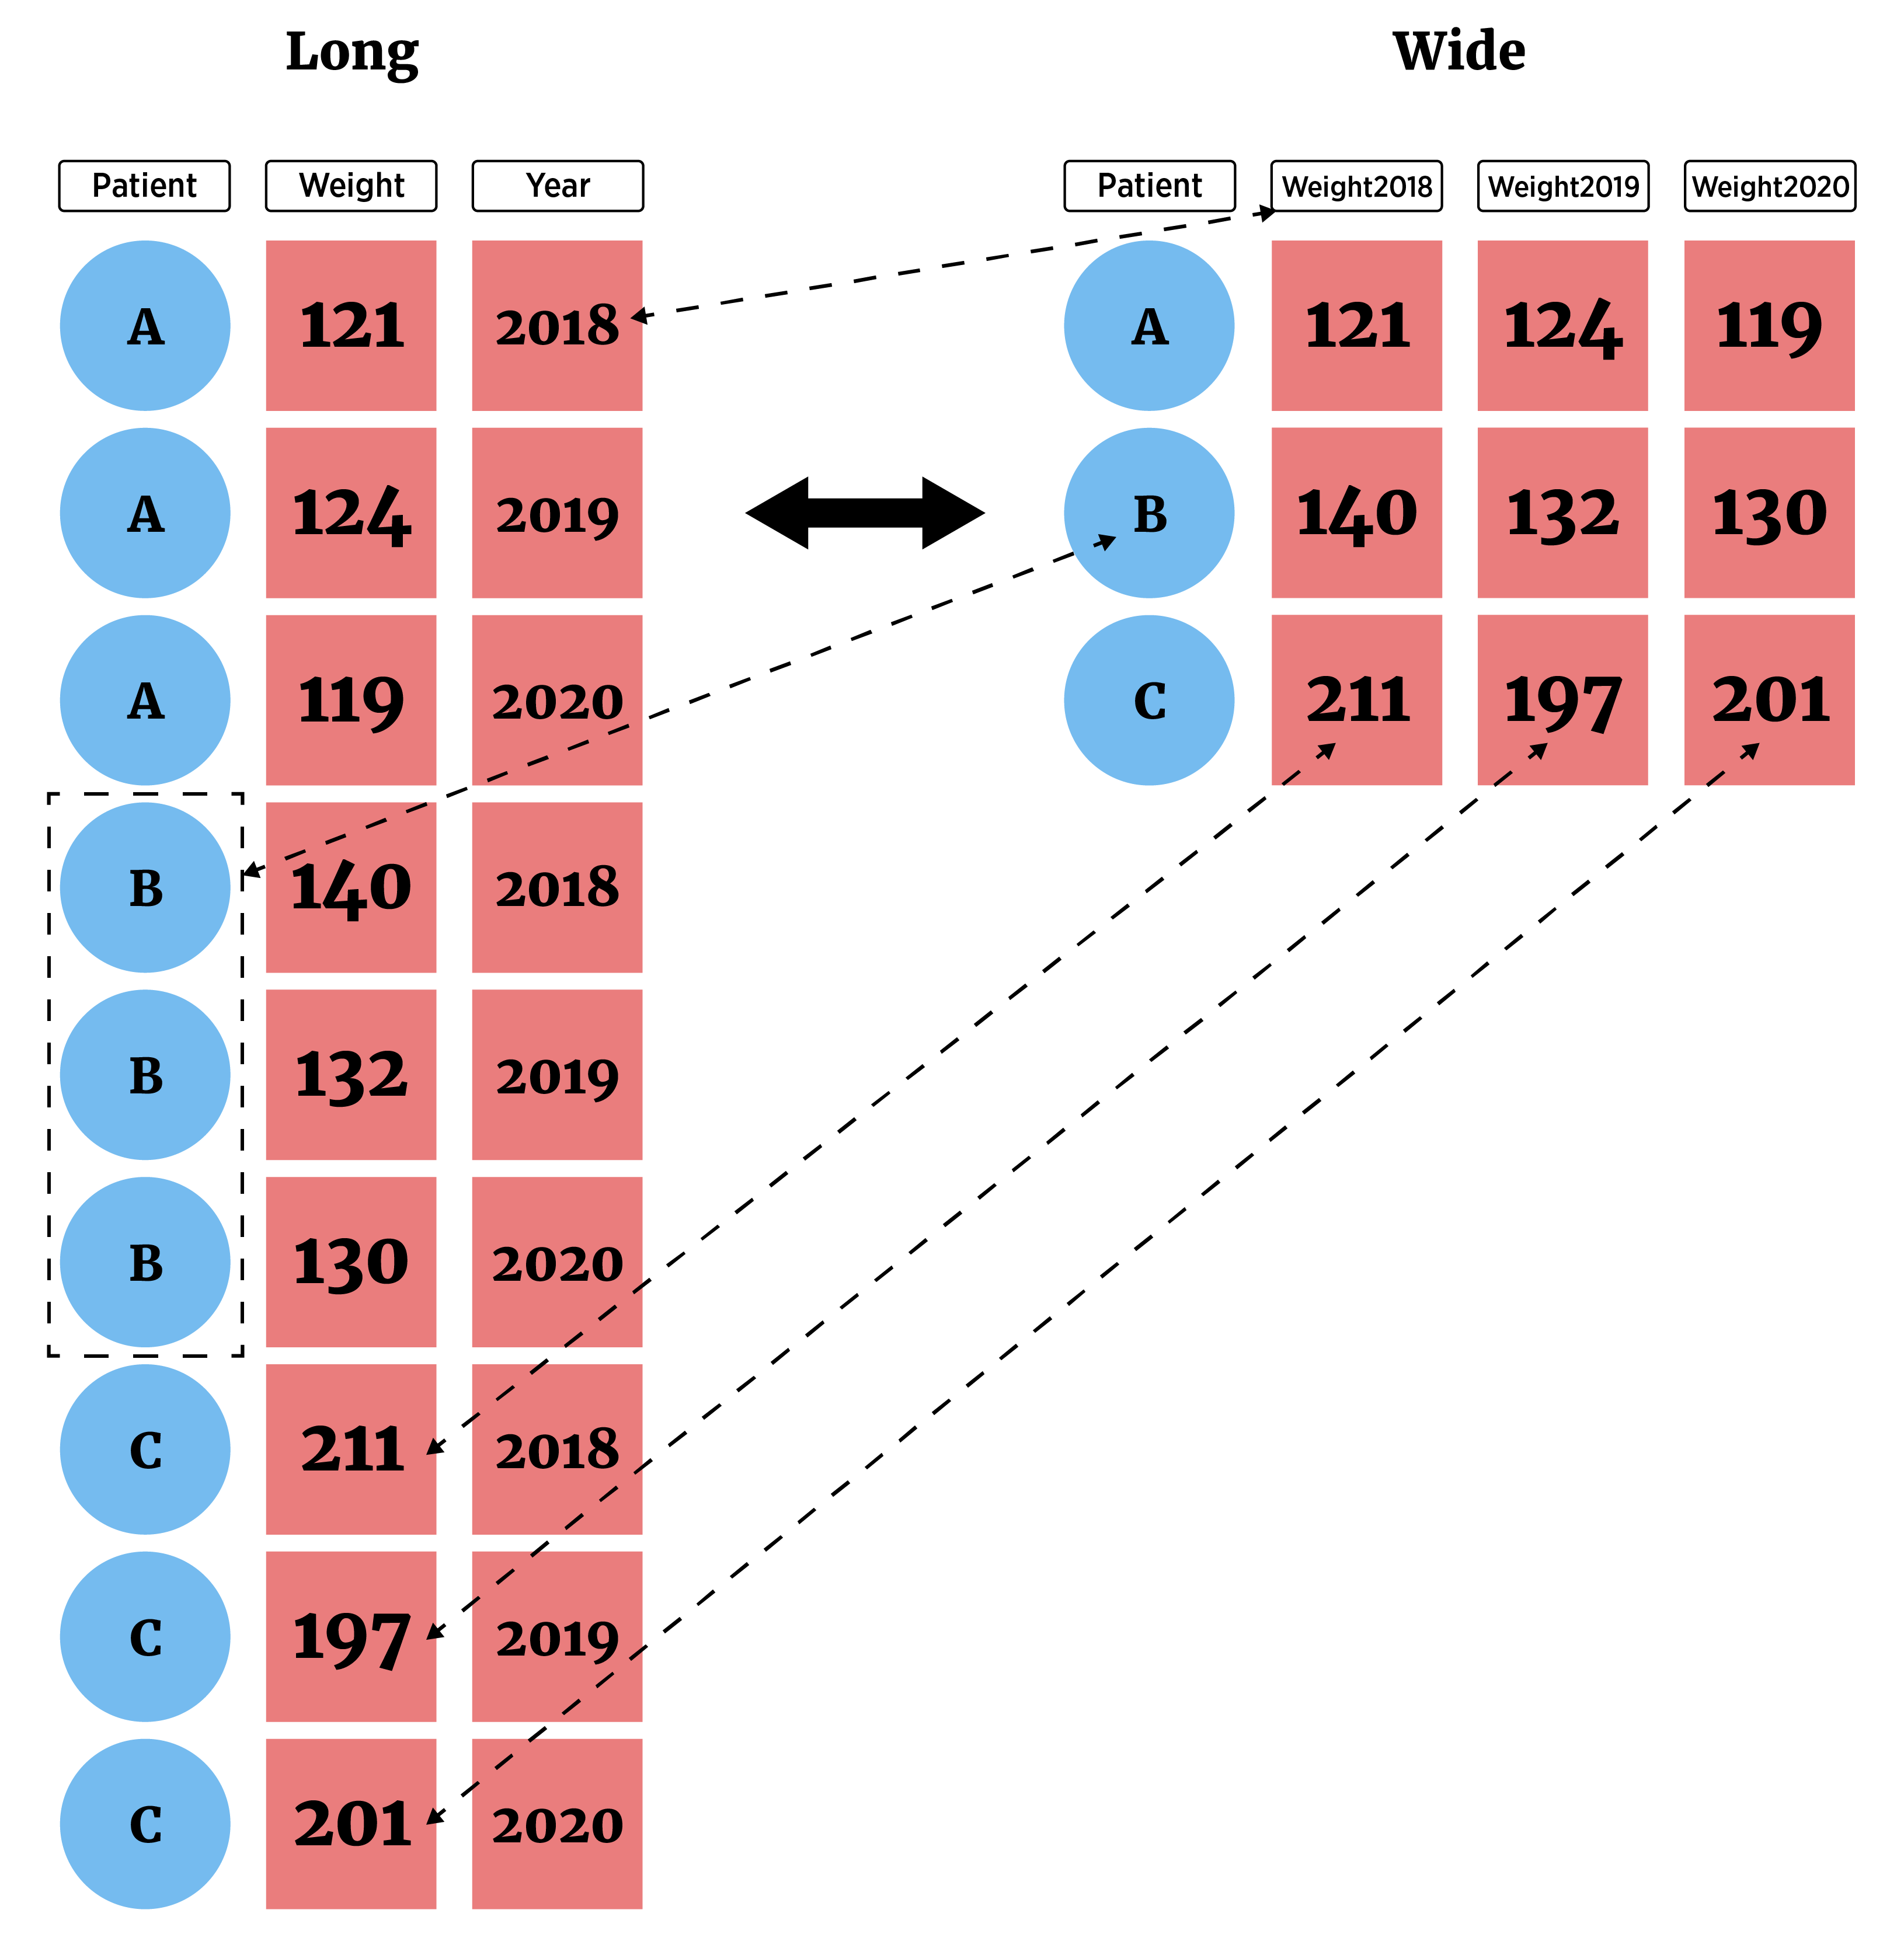
\includegraphics[width=0.7\linewidth]{img/longWideF} \end{center}

Data may have observations across some columns since viewing data is often more natural that way. For example, consider the weather data set below.

\begin{Shaded}
\begin{Highlighting}[]
\NormalTok{tempsData <-}\StringTok{ }\KeywordTok{read_table2}\NormalTok{(}\DataTypeTok{file =} \StringTok{"https://www4.stat.ncsu.edu/~online/datasets/cityTemps.txt"}\NormalTok{) }
\NormalTok{tempsData}
\end{Highlighting}
\end{Shaded}

\begin{verbatim}
## Parsed with column specification:
## cols(
##   city = col_character(),
##   sun = col_double(),
##   mon = col_double(),
##   tue = col_double(),
##   wed = col_double(),
##   thr = col_double(),
##   fri = col_double(),
##   sat = col_double()
## )
\end{verbatim}

\begin{verbatim}
## # A tibble: 6 x 8
##   city        sun   mon   tue   wed   thr   fri   sat
##   <chr>     <dbl> <dbl> <dbl> <dbl> <dbl> <dbl> <dbl>
## 1 atlanta      81    87    83    79    88    91    94
## 2 baltimore    73    75    70    78    73    75    79
## 3 charlotte    82    80    75    82    83    88    93
## 4 denver       72    71    67    68    72    71    58
## 5 ellington    51    42    47    52    55    56    59
## 6 frankfort    70    70    72    70    74    74    79
\end{verbatim}

This data set is said to be in `wide' format because columns represent observations. For most analyses this type of data will need to be reshaped into long format. The \texttt{tidyr} package can be used for this purpose!

The \texttt{gather} function takes multiple columns and gathers them into key-value pairs. This tkes wide data and makes it long.

Similarly there is a \texttt{spread} function takes two columns (key \& value) and spreads in to multiple columns. This takes long data and makes it wide.

Let's switch the tempsData dataset to `long' form with \texttt{gather()}. We need to identify the

\begin{itemize}
\item
  key = new name for values in columns
\item
  value = new name for data values
\item
  columns describe which columns to take
\end{itemize}

\begin{Shaded}
\begin{Highlighting}[]
\NormalTok{tempsData }\OperatorTok\StringTok{ }\KeywordTok{gather}\NormalTok{(}\DataTypeTok{key =}\NormalTok{ day, }\DataTypeTok{value =}\NormalTok{ temp, }\DecValTok{2}\OperatorTok{:}\DecValTok{8}\NormalTok{)}
\end{Highlighting}
\end{Shaded}

\begin{verbatim}
## # A tibble: 42 x 3
##   city      day    temp
##   <chr>     <chr> <dbl>
## 1 atlanta   sun      81
## 2 baltimore sun      73
## 3 charlotte sun      82
## 4 denver    sun      72
## 5 ellington sun      51
## # ... with 37 more rows
\end{verbatim}

The columns can be provided to gather in similar ways to how we chose them in the \texttt{select} function.

\begin{Shaded}
\begin{Highlighting}[]
\NormalTok{newTempsData <-}\StringTok{ }\NormalTok{tempsData }\OperatorTok\StringTok{ }\KeywordTok{gather}\NormalTok{(}\DataTypeTok{key =}\NormalTok{ day, }\DataTypeTok{value =}\NormalTok{ temp, sun}\OperatorTok{:}\NormalTok{sat)}
\NormalTok{newTempsData}
\end{Highlighting}
\end{Shaded}

\begin{verbatim}
## # A tibble: 42 x 3
##   city      day    temp
##   <chr>     <chr> <dbl>
## 1 atlanta   sun      81
## 2 baltimore sun      73
## 3 charlotte sun      82
## 4 denver    sun      72
## 5 ellington sun      51
## # ... with 37 more rows
\end{verbatim}

To give an example of using \texttt{spread} we can take our long format data and turn it back into wide format. WE just need to identify the:

\begin{itemize}
\item
  key = new column names
\item
  value = value to spread out
\end{itemize}

\begin{Shaded}
\begin{Highlighting}[]
\NormalTok{newTempsData }\OperatorTok\StringTok{ }\KeywordTok{spread}\NormalTok{(}\DataTypeTok{key =}\NormalTok{ day, }\DataTypeTok{value =}\NormalTok{ temp)}
\end{Highlighting}
\end{Shaded}

\begin{verbatim}
## # A tibble: 6 x 8
##   city        fri   mon   sat   sun   thr   tue   wed
##   <chr>     <dbl> <dbl> <dbl> <dbl> <dbl> <dbl> <dbl>
## 1 atlanta      91    87    94    81    88    83    79
## 2 baltimore    75    75    79    73    73    70    78
## 3 charlotte    88    80    93    82    83    75    82
## 4 denver       71    71    58    72    72    67    68
## 5 ellington    56    42    59    51    55    47    52
## 6 frankfort    74    70    79    70    74    72    70
\end{verbatim}

The \texttt{tidyr} package also has useful functions for separating a column (or combining two columns) using \texttt{separate} (and \texttt{unite})

\begin{center}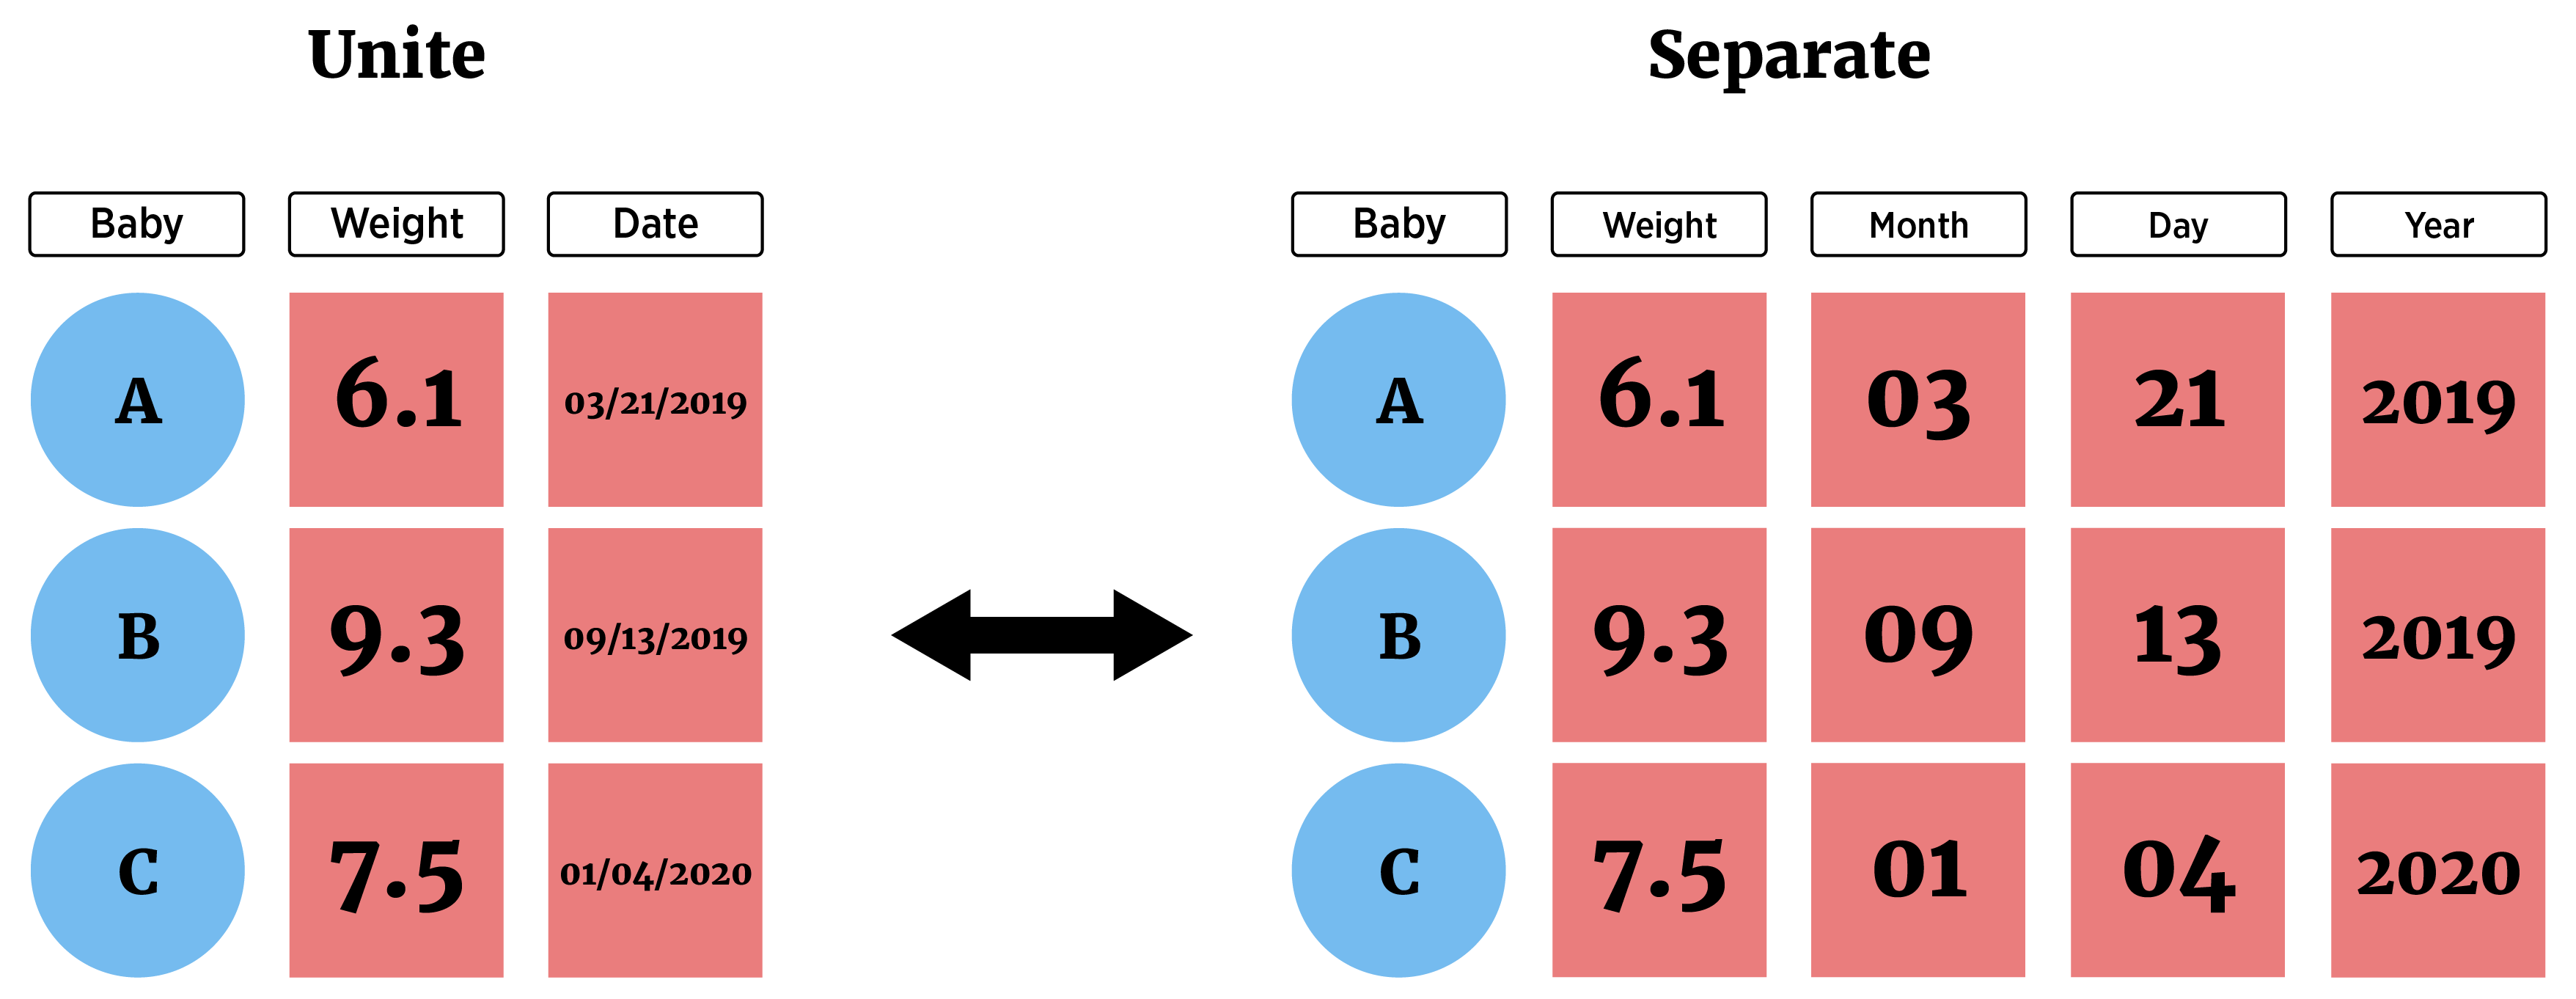
\includegraphics[width=0.8\linewidth]{img/uniteSeparateF} \end{center}

Consider a data set on air pollution in Chicago.

\begin{Shaded}
\begin{Highlighting}[]
\NormalTok{chicagoData <-}\StringTok{ }\KeywordTok{read_csv}\NormalTok{(}\StringTok{"https://www4.stat.ncsu.edu/~online/datasets/Chicago.csv"}\NormalTok{)}
\NormalTok{chicagoData}
\end{Highlighting}
\end{Shaded}

\begin{verbatim}
## Parsed with column specification:
## cols(
##   X = col_double(),
##   city = col_character(),
##   date = col_character(),
##   death = col_double(),
##   temp = col_double(),
##   dewpoint = col_double(),
##   pm10 = col_double(),
##   o3 = col_double(),
##   time = col_double(),
##   season = col_character(),
##   year = col_double()
## )
\end{verbatim}

\begin{verbatim}
## # A tibble: 1,461 x 11
##       X city  date     death  temp dewpoint  pm10    o3  time season  year
##   <dbl> <chr> <chr>    <dbl> <dbl>    <dbl> <dbl> <dbl> <dbl> <chr>  <dbl>
## 1  3654 chic  1/1/1997   137  36       37.5  13.1  5.66  3654 winter  1997
## 2  3655 chic  1/2/1997   123  45       47.2  41.9  5.53  3655 winter  1997
## 3  3656 chic  1/3/1997   127  40       38    27.0  6.29  3656 winter  1997
## 4  3657 chic  1/4/1997   146  51.5     45.5  25.1  7.54  3657 winter  1997
## 5  3658 chic  1/5/1997   102  27       11.2  15.3 20.8   3658 winter  1997
## # ... with 1,456 more rows
\end{verbatim}

The \texttt{lubridate} package great for date data but let's just do some basic parsing of the \texttt{date} variable using \texttt{separate}. We can split the \texttt{date} variable by the \texttt{/} that separates the day, month, and year to create three new columns. Using \texttt{remove\ =\ FALSE} keeps the original variable (\texttt{date}) and \texttt{convert\ =\ TRUE} attempts to convert the newly created variables to numeric if possible.

\begin{Shaded}
\begin{Highlighting}[]
\NormalTok{chicagoData }\OperatorTok\StringTok{ }\KeywordTok{separate}\NormalTok{(date, }\KeywordTok{c}\NormalTok{(}\StringTok{"Day"}\NormalTok{, }\StringTok{"Month"}\NormalTok{, }\StringTok{"Year"}\NormalTok{), }\DataTypeTok{sep =} \StringTok{"/"}\NormalTok{, }
                                                 \DataTypeTok{convert =} \OtherTok{TRUE}\NormalTok{, }\DataTypeTok{remove =} \OtherTok{FALSE}\NormalTok{)}
\end{Highlighting}
\end{Shaded}

\begin{verbatim}
## # A tibble: 1,461 x 14
##       X city  date    Day Month  Year death  temp dewpoint  pm10    o3  time
##   <dbl> <chr> <chr> <int> <int> <int> <dbl> <dbl>    <dbl> <dbl> <dbl> <dbl>
## 1  3654 chic  1/1/~     1     1  1997   137  36       37.5  13.1  5.66  3654
## 2  3655 chic  1/2/~     1     2  1997   123  45       47.2  41.9  5.53  3655
## 3  3656 chic  1/3/~     1     3  1997   127  40       38    27.0  6.29  3656
## 4  3657 chic  1/4/~     1     4  1997   146  51.5     45.5  25.1  7.54  3657
## 5  3658 chic  1/5/~     1     5  1997   102  27       11.2  15.3 20.8   3658
## # ... with 1,456 more rows, and 2 more variables: season <chr>, year <dbl>
\end{verbatim}

Similarly we can combine columns with \texttt{unite}. Let's create a new column that is just the day and month separated by a \texttt{-}.

\begin{Shaded}
\begin{Highlighting}[]
\NormalTok{chicagoData }\OperatorTok\StringTok{ }\KeywordTok{separate}\NormalTok{(date, }\KeywordTok{c}\NormalTok{(}\StringTok{"Day"}\NormalTok{, }\StringTok{"Month"}\NormalTok{, }\StringTok{"Year"}\NormalTok{), }\DataTypeTok{sep =} \StringTok{"/"}\NormalTok{, }
                                                 \DataTypeTok{convert =} \OtherTok{TRUE}\NormalTok{, }\DataTypeTok{remove =} \OtherTok{FALSE}\NormalTok{) }\OperatorTok
\StringTok{  }\KeywordTok{unite}\NormalTok{(DayMonth, Day, Month, }\DataTypeTok{sep =} \StringTok{"-"}\NormalTok{)}
\end{Highlighting}
\end{Shaded}

\begin{verbatim}
## # A tibble: 1,461 x 13
##       X city  date  DayMonth  Year death  temp dewpoint  pm10    o3  time season
##   <dbl> <chr> <chr> <chr>    <int> <dbl> <dbl>    <dbl> <dbl> <dbl> <dbl> <chr> 
## 1  3654 chic  1/1/~ 1-1       1997   137  36       37.5  13.1  5.66  3654 winter
## 2  3655 chic  1/2/~ 1-2       1997   123  45       47.2  41.9  5.53  3655 winter
## 3  3656 chic  1/3/~ 1-3       1997   127  40       38    27.0  6.29  3656 winter
## 4  3657 chic  1/4/~ 1-4       1997   146  51.5     45.5  25.1  7.54  3657 winter
## 5  3658 chic  1/5/~ 1-5       1997   102  27       11.2  15.3 20.8   3658 winter
## # ... with 1,456 more rows, and 1 more variable: year <dbl>
\end{verbatim}

You should now be ready to use R to get data in and do some basic manipulation!

\hypertarget{sas}{%
\section{SAS}\label{sas}}

The general workflow for programming in SAS is similar to that of R. First raw data must be imported to SAS. Once that data is imported you will find an appropriate PROC (or procedure) that will summarize or analyze your data appropriate. Often times relevant graphs and summaries are created with a single PROC.

At the end of this section the reader should be able to do the following:

\begin{itemize}
\tightlist
\item
  install SAS University Edition\\
\item
  read and write basic SAS programs\\
\item
  import well-formatted data into SAS
\item
  do basic data manipulation in SAS
\end{itemize}

As the book progresses the steps of summarizing and analyzing the data will be covered. Let's get started!

\hypertarget{basics-of-sas}{%
\subsection{Basics of SAS}\label{basics-of-sas}}

\hypertarget{reading-data-with-sas}{%
\subsection{Reading Data with SAS}\label{reading-data-with-sas}}

\hypertarget{manipulating-data-with-sas}{%
\subsection{Manipulating Data with SAS}\label{manipulating-data-with-sas}}

\hypertarget{sampling-experiments-and-exploratory-data-analysis}{%
\chapter{Sampling, Experiments, and Exploratory Data Analysis}\label{sampling-experiments-and-exploratory-data-analysis}}

\hypertarget{data-in-the-wild}{%
\section{Data in the Wild}\label{data-in-the-wild}}

Data is a collection of information about a group, which may include both quantitative and qualitative variables. Data is ubiquitous in today's society. Healthcare, marketing, history, biology, \ldots{} basically, every field has a quantitative aspect. However, the quality of data varies greatly from study to study and this implies the conclusions which you can draw from a study vary as well.

\hypertarget{data-from-experiments}{%
\subsection{Data from Experiments}\label{data-from-experiments}}

Some data comes from a well-designed experiment where a researcher uses sound principles to select units and conduct interventions.

For example, a mechanical engineer wants to determine which variables influence the overall gas mileage of a certain year and model of a car. Gas mileage would be referred to as the \textbf{response} variable for this study.

After careful consideration, the engineer chooses to investigate a few \textbf{explanatory variables}. They looked at the following \textbf{factors} that they believed may affect the overall gas mileage:

\begin{itemize}
\tightlist
\item
  Tire pressure (low, standard)\\
\item
  Octane rating of fuel (regular, midgrade, premium)\\
\item
  Type of driving (defensive, aggressive)
\end{itemize}

They also choose to \textbf{control} or hold constant the following variables during the implementation of the study:

\begin{itemize}
\tightlist
\item
  Weather conditions\\
\item
  Route\\
\item
  Tire type\\
\item
  Past car usage
\end{itemize}

The engineer randomly selects 24 cars from the assembly line for that year and model of car (we'll learn more about the importance of selecting a representative sample of cars shortly). Software is used to randomly assign a \textbf{treatment} or combination of the factors to each car of the 24 cars. For instance, low tire pressure, regular octane fuel, and defensive driving would be a treatment. The cars would be called the \textbf{experimental units} or (EUs) as they are the unit the treatments are assigned to.

The experiment is run and the gas mileage found for each car. As the car is being measured we'd refer to the car as the \textbf{observational unit}.

This short description exhibits three important concepts in experimental design that we'll come back to many times.

\BeginKnitrBlock{definition}
Experimental Study - researchers manipulate the conditions in which the study is done.
\EndKnitrBlock{definition}

Pillars of experimental design: (Put an outer block around this)

\BeginKnitrBlock{definition}
\begin{itemize}
\tightlist
\item
  Randomization - treatments are randomly assigned to the experimental units\\
\end{itemize}
\EndKnitrBlock{definition}

\BeginKnitrBlock{definition}
\begin{itemize}
\tightlist
\item
  Replication - multiple (independent) experimental units are assigned the same treatment\\
\end{itemize}
\EndKnitrBlock{definition}

\BeginKnitrBlock{definition}
\begin{itemize}
\tightlist
\item
  Control - study conditions are held constant where possible to reduce variability in the response\\
\end{itemize}
\EndKnitrBlock{definition}

\hypertarget{data-from-observational-studies}{%
\subsection{Data from Observational Studies}\label{data-from-observational-studies}}

Some data comes from an observational study where the researcher collects data without imposing any changes.

For example, an economist wants to investigate the effects of recently added tariffs on agricultural products to the amount and value of such products that are traded between the United States and Asia. This study would have two \textbf{response} variables, the amount and value of each product traded between the two parties.

In order to take into account season variation and time of year, the economist decides to compare the two response variables from the current year - 6 months worth of data - to the \emph{average} values of the two response variables during the same 6 month periods for the past 5 years. We would refer to the time frame of the data as an \textbf{explanatory variable}. This time frame could be labeled to take on one of two values: no-tariff (past) or tariff (current).

The researcher obtains the data from the census bureau and conducts their analysis.

Notice that the researcher, while certainly being actively involved in the careful consideration of the data to be collected, does not actively intervene or impose a change. This is the key component of an observational study.

\BeginKnitrBlock{definition}
Observational Study - researchers collect data without imposing any changes on the study environment.
\EndKnitrBlock{definition}

\hypertarget{observational-vs-experimental}{%
\subsection{Observational vs Experimental}\label{observational-vs-experimental}}

You may have noticed that both types of studies have some things in common. For instance, both studies have \textbf{response} (??? so I was thinking about maybe bolding most stats words as we go to point them out to students\ldots{} thoughts???) variables that characterize the performance of the study in some sense. Importantly, these response variables have variation. That is, observing the variable is non-deterministic even under identical situations. There are also \textbf{explanatory variables} that the researcher is interested in with regard to their relationship with the response variable.

Beyond that, both studies hope to make conclusions about a larger group using data. This is the idea of \textbf{statistical inference} (??? Do we want to talk about the differences between prediction and inference here? - later???). More formally the group of values, items, or individuals defines the the \textbf{population} of interest and the data collected represents the \textbf{sample}. For the gas mileage example, the population would be all cars of the year and make in question and the sample would be the data on the 24 cars. For the tariff example, the population would be a \textbf{conceptual population} of all future agricultural products traded between the United States and Asia and the sample would be the information from the six years of trade data.

\BeginKnitrBlock{definition}
Population - (Possibly conceptual) group of units of interest
\EndKnitrBlock{definition}

\BeginKnitrBlock{definition}
Sample - Subset of the population on which we observe data
\EndKnitrBlock{definition}

\BeginKnitrBlock{definition}
Statistical Inference - Process of using sample data to make statements or claims about a population (???Usually with the goal of determining which variables are important for a response???)
\EndKnitrBlock{definition}

Both of these studies had to determine how to obtain their observations. For the experiment, 24 cars were used. For the observational study, six years of data were collected. How this data is collected can be extremely important in terms of the types of conclusions that can be made. Data needs to be \textbf{unbiased} and \textbf{representative} of the population in which the researcher hopes to make inference otherwise the conclusions made are likely invalid. We'll discuss the idea of what makes a good and bad \textbf{sampling scheme} later.

The major difference between the two studies was the active (experimental) and passive (observational) roles played by the researcher. This difference is also of vital importance to the types of conclusions that can be made from the study. A well-designed experiment can often infer causation to the treatments where an observational study cannot.

The conclusions a researcher can make based on how the data were collected and the type of study are outlined in the table below. (??? Probably just remake this table ourselves with our own words. This isn't exactly `their' original thought or something we need to attribute. ???)

\begin{figure}
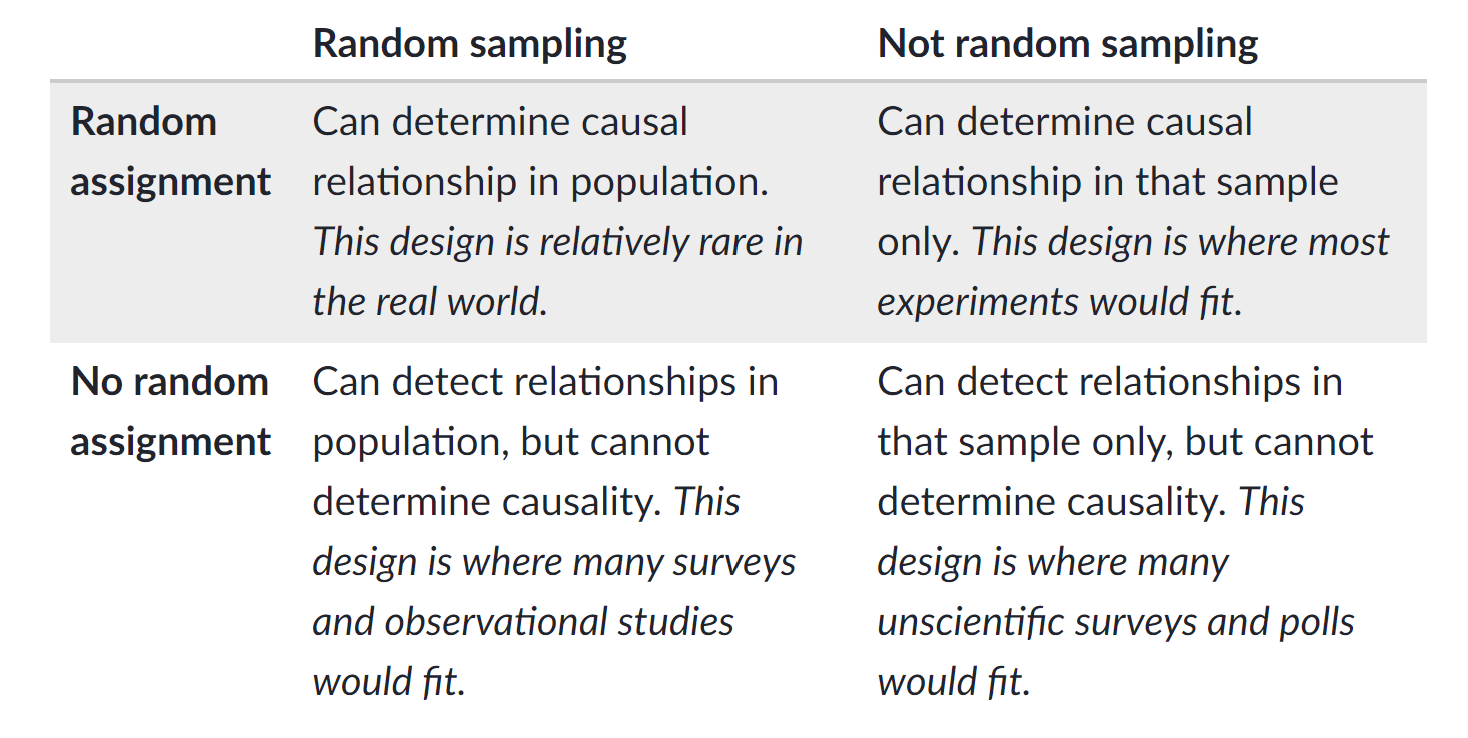
\includegraphics[width=0.8\linewidth]{img/ScopeOfInferenceTable} \caption{Scope of Inference, cite: Khan Academy}\label{fig:scope}
\end{figure}

Doing an observational study doesn't mean that your study is bad! An observational study is sometimes done out of necessity when an experiment wouldn't be ethical or feasible. For the tariff example, there really isn't a way to conduct an experiment. If we wanted to design an experiment to see if smoking causes lung cancer, that would be unethical because we can't force people to smoke. The key point is that the implications we can draw will differ greatly between experimental and observational studies and will depend heavily on the quality (in relation to the population) of the data you have.

\hypertarget{the-role-of-statistics}{%
\subsection{The Role of Statistics}\label{the-role-of-statistics}}

Statistics is the science of learning from data. It encompasses the collection of data, the design of an experiment, the summarization of data, and the modeling or analysis used in order to make a decision or further scientific knowledge. (???I feel like this definition doesn't quite get the sampling part right or maybe the holistic process or something - update as needed! JP???)

\BeginKnitrBlock{definition}
(This will be changed to a different style of callout - maybe ``note''?)

Statistics in everyday use usually refers to simply summaries about data (means/averages, proportions, or counts).

Statistics as a field encompasses a much larger range of ideas including how to collect data, model data, and make decisions or come to conclusions when faced with uncertainty.
\EndKnitrBlock{definition}

\textbf{Statistical methods are needed because data is variable.} If we again collected data about the gas mileage of vehicles under the exact same study conditions we'll get slightly different results. If we observed another six month period of trade data we'll see different amounts and values. Accounting for this variability in data is a key component of a statistical analysis.

Generally, one should try to take a holistic view of a study. Before any data is collected it is vital to understand the goals and background of the study. These will inform the data you ideally want to collect as well as the data that you are able to collect - which may need to act as a proxy. A plan should be determined for the actual collection and storing of the data. The entire study design will then inform the statistical analysis and conclusions that can be drawn.

Taking this bigger picture view of the problem, we can usually follow these steps (we'll try to follow these throughout the book!):

\begin{itemize}
\tightlist
\item
  Define the objective of the experiment and understand the background (Define Objective \& Background)\\
\item
  Select appropriate response variables (Select Response)\\
\item
  Identify sources of variation (Determine Sources of Variation)\\
\item
  Choose sampling scheme and/or experimental design (Select Design)\\
\item
  Carry out the study (Do Study)
\item
  Statistically analyze the data (Do Statistical Analysis)\\
\item
  Draw conclusions from the analysis while considering limitations and the steps above as well as communicate results (Draw Conclusions \& Communicate)
\end{itemize}

We'll focus on this entire process in our big chapter examples and mostly investigate designed experiments. We attempt to tackle each topic in this text with a problem-based approach. That is, we identify a real-world problem and discuss the relevant statistical ideas in context. At the end of each chapter, we provide a recap of the main statistical ideas and discuss other important related topics. Where applicable we include a section that outlines some of the mathematical concepts as well as a section to outline software related to the topic.

\hypertarget{descriptive-study---farmers-market}{%
\section{Descriptive Study - Farmer's Market}\label{descriptive-study---farmers-market}}

\hypertarget{define-objective-background}{%
\subsection{Define Objective \& Background}\label{define-objective-background}}

A nutrition scientist wanted to understand the cleanliness and food hygiene of the vendors at the North Carolina State Farmer's Market (henceforth the farmer's market). Secondarily, she wanted to learn about vendor sales to see if there was a relationship with their cleanliness and food hygiene. The researcher had access to the names of each vendor's business, their general purpose, and the products they sold.

The researcher needed to decide the scope of their study. Formally, they needed to define the \textbf{population} of interest. The population is the group of people or units of interest to the researcher. As her interest centered around food-related businesses, she restricted to looking at the vendors which sold horticultural crops. She hoped that conclusions made by her study could apply to all horticulture vendors at the farmer's market - thus, this is her population.

Note: One could try to do a study at just the North Carolina State Farmer's Market and extend the results to all farmer's markets in the state or in the south, but that would require many assumptions to be valid.

A \href{http://www.ncagr.gov/markets/chart.htm}{list of the horticultural products sold and their is availability} is reproduced below.

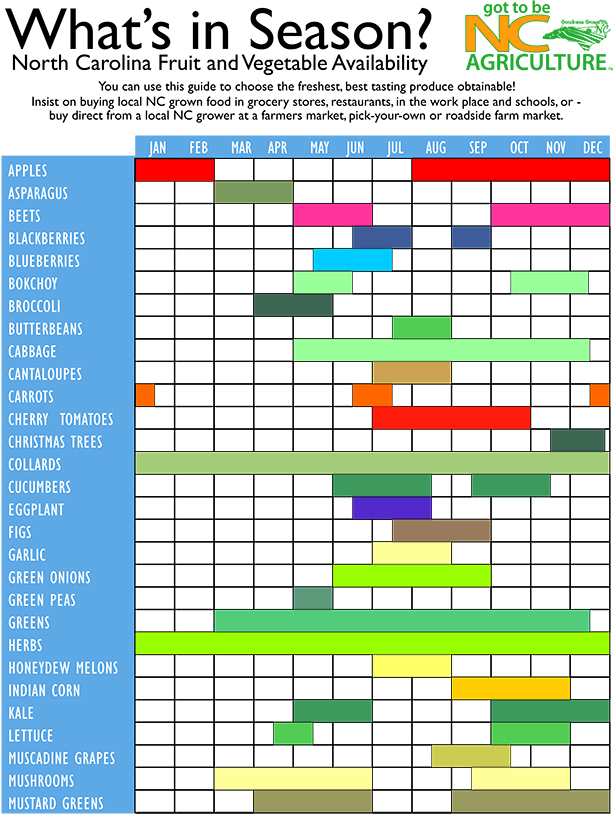
\includegraphics[width=0.65\linewidth]{img/availabilitychart-1}
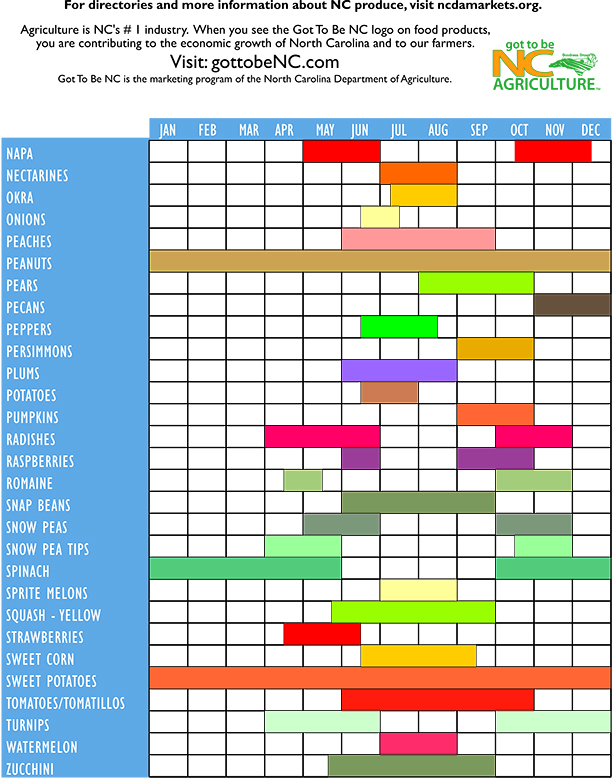
\includegraphics[width=0.65\linewidth]{img/availabilitychart-2}

\hypertarget{select-response}{%
\subsection{Select Response}\label{select-response}}

The researcher needed to determine the variables to collect that would best help to answer their questions of interest. These variables that characterize the experiment are called \textbf{response} or target variables.

To investigate the knowledge of hygiene and safety, a short questionnaire was developed to allow the vendor's head manager (or similar employee) to describe their safety protocol and knowledge:

\begin{itemize}
\tightlist
\item
  For your produce with signs that say ``clean'' or ``washed'', what does this mean?
\item
  How are the foods transported to the market? eg: refrigerated/closed storage\\
\item
  What food safety risks do you as a vendor worry about?\\
\item
  Do you require one-use gloves to be used? (Yes or No)\\
\item
  Do you designate a person in charge of money transactions? (Yes or No)
\end{itemize}

The researcher also planned to do an assessment of the cleanliness of each vendor's station at different times. Her team would pick 30 days during the summer in which they'd walk through the vendor stations and collect the following information:

\begin{itemize}
\tightlist
\item
  Overall is the station clean (Yes or No)\\
\item
  Is anyone smoking around the food products? (Yes or No)\\
\item
  Are tables covered? (Yes or No) If so, what is the material?\\
\item
  Do employees appear to be clean? (Yes or No)\\
\item
  Are one-use gloves used? (Yes or No)\\
\item
  Is there a designated person in charge of money transactions (Yes or No)
\end{itemize}

She noted that there is a yearly cycle to the products sold and decided to collect vendors sales information by looking at the (AMT) amount sold in the last year (in dollars), the (PURCHASE) total number of purchases made in the last year, and the (NUM\_ITEMS) total number of items sold in the last year. For the last variable, they had to decide how to measure the number of items sold for the different types of crops. For most of the crops looking at the total weight (in lbs) sold made sense. But, for some, other measures were needed. For example, for sweet corn the number of ears sold would be recorded.

You can see that there are many decisions that the researcher must make in simply deciding the response variables to collect! A poor choice here can make or break a study.

\hypertarget{determine-sources-of-variation}{%
\subsection{Determine Sources of Variation}\label{determine-sources-of-variation}}

The response variables clearly have some relationship to other variables that could be collected. For instance, the NUM\_ITEMS variable is clearly going to be different based upon what crops the vendor sells. The AMT variable would differ depending on the size of the vendor's inventory. These are examples of \textbf{explanatory variables} or variables that define the study conditions. Explanatory variables go by many names such as predictors, features, or independent variables.

\textbf{A main consideration about whether or not to record a variable is whether or not the variable would be related to a variation in a response variable.} Since the response variables are truly what is of interest, there is really not much of a point in recording variables that likely have no relationship with it.

Choosing the explanatory variables can also indicate further questions of interest. For instance, the researcher may want to compare the percent of ``Yes'' for the overall cleanliness score for vendors that mainly sell vegetables to those that mainly sell fruit leading to a comparison across groups being of interest. She may want to try to model the AMT of cantaloupe sold as a function of the cleanliness score.

The average amount for the population or a subpopulation would be referred to as a parameter of interest. Formally, a \textbf{parameter} is a summary measure about a population. Common parameters investigated include a mean, proportion, median, or variance of different subgroups of the population.

The explanatory variables she collected about the vendors included the types of crops sold, the services they provide (grow, pack, and/or ship), and whether or not they are a ``Got to be NC member''.

For the questionnaire, she added the additional questions below:

\begin{itemize}
\tightlist
\item
  Are there any organic or synthetic chemicals/fertilizers/pesticides/manures used on the products?\\
\item
  Are all foods grown/processed by the vendors?\\
\item
  What kind of soil were the products grown in? eg: organic/compost/plant material
\end{itemize}

For the assessment of cleanliness, she added the following question:

\begin{itemize}
\tightlist
\item
  How many people are working?
\end{itemize}

\textbf{Should we talk about formalizing the other questions they want to answer here??}

\hypertarget{select-design}{%
\subsection{Select Design}\label{select-design}}

For this study the researchers aren't interested in doing an intervention so an observational study was being done. The major task to consider for the observational study is how to select participants from the population. The subset of the population we (attempt to) observe our data on is called the \textbf{sample}. The \textbf{sample size} is the number of measurements in the sample.

Ideally, we would measure every member of our population. This is called a \textbf{census}. If a census can be done then the value of a population's parameter can be found exactly by simply summarizing the population data. However, conducting a census can be extremely costly or time-intensive so most of the time a census cannot be done. This means that the information we collect would likely be different if we collected it again. Accounting for this variability is the main reason statistical analysis is needed.

How the researcher selects their sample is extremely important. This method is often referred to as the \textbf{sampling scheme}. Using a statistically valid sampling scheme is vital to the assumptions made when doing statistical inference. A valid sampling scheme implies that every member of the population has a known and non-zero chance of inclusion in the sample.

There are many good ways to select the sample and many bad ways. \textbf{Need to get more info about the farmer's market to finish this part}
(Talk about bad first and why bad - visuals too) Talk about good and why good - visuals too.

This idea is further fleshed out at the end of the chapter. (reference/link this)

Here they chose to do a stratified sample to make sure that they didn't leave out any important subgroups.

\textbf{Should we talk about formalizing the other questions they want to answer here??}

\hypertarget{do-study}{%
\subsection{Do Study}\label{do-study}}

Go and talk to chosen vendors. May have some non-response issues. Ideally a contingency for this should be developed when considering the sampling scheme.

\textbf{Should we talk about formalizing the other questions they want to answer here??}

\hypertarget{do-statistical-analysis}{%
\subsection{Do Statistical Analysis}\label{do-statistical-analysis}}

\textbf{Should we talk about formalizing the other questions they want to answer here??}

The major goals of this study were simply to describe the vendors at the farmer's market. In this case we can produce numerical and graphical summaries.

Careful discussion of not selecting a modeling technique based on this unless it is a pilot study or an exploratory study else we have increased our nominal type I error rate\ldots{}

Spend a lot of time here talking about graphs of different types. Sample means, sample variances, etc.

Discuss population curves vs sample histograms and the relationship.

Not a formal test here but comparisons of interest etc.

\hypertarget{draw-conclusions-communicate}{%
\subsection{Draw Conclusions \& Communicate}\label{draw-conclusions-communicate}}

What actionable things have we found? Likely some trends to investigate further. Perhaps run an experiment to formally see if some alteration can be effective.

What can we conclude realistically from this data? To what population are we talking?

\hypertarget{statistical-testing-ideas---simulated-experiment}{%
\section{Statistical Testing Ideas - Simulated Experiment}\label{statistical-testing-ideas---simulated-experiment}}

\hypertarget{define-objective-background-1}{%
\subsection{Define Objective \& Background}\label{define-objective-background-1}}

\hypertarget{select-response-1}{%
\subsection{Select Response}\label{select-response-1}}

\hypertarget{determine-sources-of-variation-1}{%
\subsection{Determine Sources of Variation}\label{determine-sources-of-variation-1}}

\hypertarget{select-design-1}{%
\subsection{Select Design}\label{select-design-1}}

\hypertarget{do-study-1}{%
\subsection{Do Study}\label{do-study-1}}

\hypertarget{do-statistical-analysis-1}{%
\subsection{Do Statistical Analysis}\label{do-statistical-analysis-1}}

\hypertarget{draw-conclusions-communicate-1}{%
\subsection{Draw Conclusions \& Communicate}\label{draw-conclusions-communicate-1}}

\hypertarget{statistical-ideas-and-concepts}{%
\section{Statistical Ideas and Concepts}\label{statistical-ideas-and-concepts}}

\hypertarget{study-purpose}{%
\subsection{Study Purpose}\label{study-purpose}}

Prediction vs inference

Param, sample, etc.

\hypertarget{summarizing-data}{%
\subsection{Summarizing Data}\label{summarizing-data}}

Terminology of variables

Numerical and graphical summaries

Sample of Random Variable's realizations, sample distribution vs population, modeling ideas

Approx probabilities and quantiles vs theoretical

Summaries of distributions (center, spread, graphs)

\hypertarget{study-types}{%
\subsection{Study Types}\label{study-types}}

Ob vs exp

Good discussion of what makes a good sampling design. Maybe a statified example like the river and selecting houses example as a quick expose of the issues with not doing a truly random sampling technique.

\hypertarget{examples-of-why-observational-studies-can-be-bad}{%
\subsubsection{Examples of why Observational Studies Can be Bad}\label{examples-of-why-observational-studies-can-be-bad}}

George Will WP column about SAT vs amount of money spent
Pisani and Perv? many bad examples of inference

\hypertarget{suggestions-for-further-readings}{%
\subsection{Suggestions for Further Readings}\label{suggestions-for-further-readings}}

\hypertarget{software-1}{%
\section{Software}\label{software-1}}

\hypertarget{r-1}{%
\subsection{R}\label{r-1}}

\hypertarget{numerical-summaries}{%
\subsubsection{Numerical Summaries}\label{numerical-summaries}}

\hypertarget{graphical-summaries}{%
\subsubsection{Graphical Summaries}\label{graphical-summaries}}

\hypertarget{sas-1}{%
\subsection{SAS}\label{sas-1}}

\hypertarget{numerical-summaries-1}{%
\subsubsection{Numerical Summaries}\label{numerical-summaries-1}}

\hypertarget{graphical-summaries-1}{%
\subsubsection{Graphical Summaries}\label{graphical-summaries-1}}

\hypertarget{point-estimates}{%
\chapter{Point Estimates}\label{point-estimates}}

Learning objectives for this lesson:
- How to estimate a mean
- Definition of ``convenience sample''
- Definition of ``systematic sample''
- Benefits/drawbacks to both approaches
- Understand how to estimate a mean
- Understand how to estimate a quantile
- Understand implicit assumptions for these approaches

\hypertarget{estiamte-with-means}{%
\section{Estiamte with means}\label{estiamte-with-means}}

\hypertarget{experiment-background}{%
\subsection{Experiment background}\label{experiment-background}}

Someone wants to know how much of something they need to satisfy some population
To get a good estimate of this, we can use the average amount for each one and then multiply by the whole population

\hypertarget{estimate-with-quantiles}{%
\section{Estimate with quantiles}\label{estimate-with-quantiles}}

\hypertarget{experiment-background-1}{%
\subsection{Experiment background}\label{experiment-background-1}}

Big Deborah's is making new packaging for their cookies. The engineer responsible for the new desing needs to make sure that the packaging fits the new cookies. While the cookie manufacturing process is standardized, there's inevitably some degree of variation in cookie size. After discussing the issue with corporate, the engineer decides that a the new cookie sleeves should be large enough to fit 95\% of cookies that are baked. (The largest five percent will be marketed separately as ``JUMBO'' cookies.)

\hypertarget{define-the-object-of-the-experiment}{%
\subsection{Define the object of the experiment}\label{define-the-object-of-the-experiment}}

The Engineer is tasked with determining how large the cooke sleeve needs to be. There's no way for her to know the size of every cookie that Big Deborah's has made (or will make going forward!), so she'll need to collect data on existing cookies to inform her cookie sleeve size determination.

\hypertarget{select-appropriate-response-variables}{%
\subsection{Select appropriate response variables}\label{select-appropriate-response-variables}}

If the maximum distance from any one point on the (round) cookie's perimeter to any other point is smaller than the diameter of the cookie sleeve, then the cookie will fit. This makes ``cookie diameter'' a good measure for this test. It is easy to measure for each cookie and is directly relevant to the experiment's objective.

{[}probably have something in here about {]}

\hypertarget{identify-sources-of-variation}{%
\subsection{IDentify sources of variation}\label{identify-sources-of-variation}}

While the manufacturing process is standardized, there is variation in size from one cookie to the next. This is one source of variation. The engineer isn't sure of any others. However, she knows that cookies are made in multiple factories, and that each factory has multiple ovens. Ovens and factories could also be sources of variation.

\hypertarget{choose-an-experimental-design}{%
\subsection{Choose an experimental design}\label{choose-an-experimental-design}}

The Engineer knows that she needs to look at multiple cookies, since she knows that there is variation in diameter from one cookie to the next. One option would be to just use the remaining cookies in the box she has in her office (22 of the 25-count box remain). {[}something about convenience sample{]} However, she knows that cookies from the same oven are typically packaged together. If there is variation from one oven to the next, looking at the cookies she has in her office may not tell the whole story.

Instead, she chooses to take every 20th cookie manufactured off the assembly line until she gets 500 cookies. {[}something about systematic sample{]}

\hypertarget{perform-the-test}{%
\subsection{Perform the test}\label{perform-the-test}}

The day of the test comes, and the Engineer starts collecting cookies. However, problems arise! The plan has to shut down half-way through, so she only gets 431 cookies instead of the 500 she thought she would. However, she measures the diameters of each cookie and records the data in a spreadsheet.

\hypertarget{statistically-analyze-the-data}{%
\subsection{Statistically analyze the data}\label{statistically-analyze-the-data}}

The initial plan had been to rank-order the 500 cookies and estimate the 95th percentile using the diamter of the 475th largets cookie. Since we didn't get all of our data, we have to improvise. 431 doesn't neatly yield a value such that exactly 95\% are less than or equal and 5\% are greater than or equal. One option is to choose the 410th largest cookie to estimate our percentile. Slightly more than 95\% of cookies will have smaller diameters than this. Alternatively, we could interpolate between the 409th and 410th cookies. {[}reasons and logic and math for each of these{]}

\hypertarget{draw-conclusions}{%
\subsection{Draw conclusions}\label{draw-conclusions}}

Based on this study, the Engineer concludes that a cookie sleeve large enough for a cookie of diameter XX will be big enough to contain 95\% of Big Deborah cookies.

\hypertarget{discussion}{%
\subsection{Discussion}\label{discussion}}

\begin{itemize}
\tightlist
\item
  pros and cons to the approach chosen
\item
  generalizing to other types of point estimates
\end{itemize}

\hypertarget{accounting-for-uncertainty}{%
\chapter{Accounting for Uncertainty}\label{accounting-for-uncertainty}}

Some \emph{significant} applications are demonstrated in this chapter.

\hypertarget{example-one}{%
\section{Example one}\label{example-one}}

\hypertarget{example-two}{%
\section{Example two}\label{example-two}}

\begin{Shaded}
\begin{Highlighting}[]
\KeywordTok{library}\NormalTok{(tidyverse)}
\end{Highlighting}
\end{Shaded}

\hypertarget{HT}{%
\chapter{Inference via Hypothesis Tests for One Sample}\label{HT}}

\hypertarget{example-detection-probability}{%
\section{Example: Detection Probability}\label{example-detection-probability}}

An important problem for the US Army is protecting soldiers in forward positions. One of main threats to these soldiers are explosive projectiles launched from great distances. These are often refered to as ``indirect fires'', since the folks launching the projectiles (``firing'' the projectiles) may not have direct visibility (``line of sight'') to their target. For example, artillery like the US M777 Light Towed Howitzer can fire projectiles over 40 km, far beyond the distance a soldier operating the machine could aim it. Instead, the gun crew relies on information about where to shoot provided to them by other units on the battlefield. This allows them to effect the battle from far away and without alerting their target.

To protect soldiers from similar threats, the US Army developed the Q-53 Counterfire Radar. One of this system's primary functions is to detect incoming indirect fires and pinpoint the source of those shots. Because soliders will be relying on the Q-53 in combat, the US Government tested it extensively to better understand how it would perform in an operational setting. The testers fired shells from systems that closely resembled the artillery that might be seen on the battlefield while actual soldiers operated a Q-53. For each shell that was fired, the testers recorded whether or not the Q-53 crew was able to detect the projectile with their system.

Using data from this test, evaluators were able to the likelihood that the Q-53 would detect an incoming projectile.

\hypertarget{understanding-system-performance}{%
\subsection{Understanding system performance}\label{understanding-system-performance}}

Let's take a step back and consider the data we're getting from this test and try to understand why the testers did things the way they did.

First, let's consider the goal of this test. At the end of the day, the US Army wants to know how effective the Q-53 is at it's job. This job is to help protect soldiers by giving them early warning if they're under attack from indirect fires like artillery. Therefore, it's vital that the Q-53 detect incoming projectiles with high probability.

Once we understand this, the choice to measure the detection probability for incoming projectiles is completley logical. This measure ties directly to the goal of the experiment. You won't always be able to find a response variable that ties so directly to the goal of your test, but when you do, rejoice.

There are some other measures the testers could've used. For example, they could've looked at how long a projectile was detected prior to its impact on the target. Similarly, they could've measured the distance from the target at time of detection. Both of these measures would give more detailed information than detection alone. However, they'd be harder to measure precisely. Addiing additional instrumentation to the Q-53 and to the test projectiles being fired at the range would add elements to the experiment that would make it less realistic. Perhaps instrumenting the projectiles would make them easier to detect. Regardless, the testers deemed the detection probability adequate to make their assessment of the system.

\hypertarget{data-analysis}{%
\subsection{Data Analysis}\label{data-analysis}}

Having identified their response variable, the testers collected data on which projectils were detected. Table 1 shows the first 20 shots collected.

\begin{Shaded}
\begin{Highlighting}[]
\NormalTok{tb <-}\StringTok{ }\NormalTok{readr}\OperatorTok{::}\KeywordTok{read_csv}\NormalTok{(}\StringTok{"datasets/Experimental/counterfire-radar/counterfire-radar.csv"}\NormalTok{) }\OperatorTok\StringTok{ }
\StringTok{  }\KeywordTok{filter}\NormalTok{(Mission }\OperatorTok\StringTok{  }\KeywordTok{c}\NormalTok{(}\DecValTok{1}\OperatorTok{:}\DecValTok{4}\NormalTok{))}

\KeywordTok{hist}\NormalTok{(tb}\OperatorTok{$}\NormalTok{Detection)}
\end{Highlighting}
\end{Shaded}

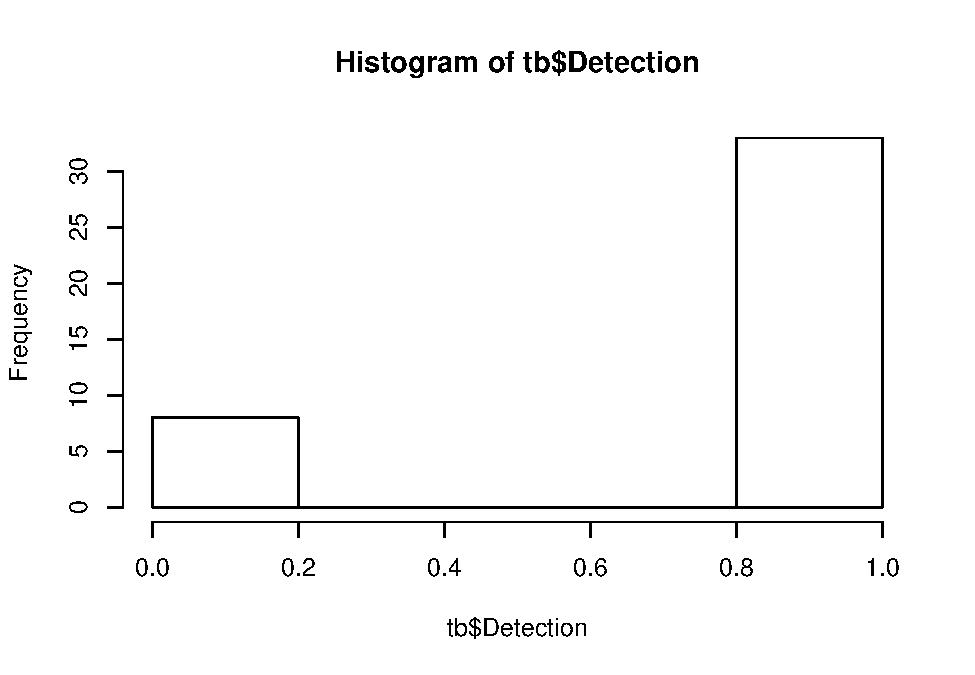
\includegraphics{StatisticalMethods_files/figure-latex/unnamed-chunk-15-1.pdf}

It's clear that the system detects these projectiles with a high probability, but what conclusions can we draw from these data? Does the system detect projectiles at a high enough rate to be useful to a commander in the field?

Typically, you'll want to think about these questions before designing a test or analyzing your data. In the case of this counterfire radar, the US Army has specified in requirements documents what it deems to be ``good enough'' in terms of detection probability. Suppose the Army requires that the system be able to detect at least 80\% of incoming projectiles.

Using that requirement, we can compare the probabiltiy of detection we observed in our sample and get an idea of whether or not the system is good enough:

\begin{Shaded}
\begin{Highlighting}[]
\NormalTok{n <-}\StringTok{ }\KeywordTok{nrow}\NormalTok{(tb)}
\NormalTok{phat <-}\StringTok{ }\KeywordTok{mean}\NormalTok{(tb}\OperatorTok{$}\NormalTok{Detection)}

\NormalTok{phat}
\end{Highlighting}
\end{Shaded}

\begin{verbatim}
## [1] 0.804878
\end{verbatim}

Let the true probability of detection for this radar system be \(\pi\), a value somewhere between \(0\) and \(1\). Then our estimate for \(\pi\) is denoted:

\[\hat\pi = \frac{1}{n}\sum_{i = 1}^n x_i\]

In this equation, \(x_i\) is 1 or a 0 depending on whether or not we detected the \(i\)th projectile, and \(n\) is the total number of observations we have. We can use this notation to state the research problem we describe above more formally: We want to determine if \(\pi > 0.8 = 80%
\). To do this, we're going to use our estimat, \(\hat \pi\).

The simplest approach is to just say that \(\hat \pi\) is our best guess for \(\pi\), so let's just ask if \(\hat \pi> 0.8\). Based on our data above, we have: \$\hat\pi = \$0.804878. This is larger than 0.8, so it looks like we're good to go!

Unforunately, \(\hat \pi\) is an \emph{estimate} of \(\pi\) and not the true value. It is based on a \emph{random sample}, which are subject to variability. Before drawing any conclusions, it's important to ask the question, ``How sure are we that \(\hat\pi\) is close to \(\pi\)?''

\hypertarget{hypothesis-testing}{%
\section{Hypothesis testing}\label{hypothesis-testing}}

The framework used throughout modern science to answer these sorts of question is known as \emph{Null Hypothesis SignificanceTesting} (NHST), or more concisely, \emph{hypothesis testing}. The basic approach is to frame our research question as a comparison between two possible realities and then decide, based on the data, if one of those realities is sufficiently implausible to discard as an actual possibility.

For our application, the two competing realities are one in which the radar's performance meets the desired performance of the Army (that is, \(\pi > 0.8\)) and one where it does not (\(\pi \le 0.8\)). These possibilities are derived directly from our research question, and are typically phrased explicitly as a \emph{Null Hypothesis} (denoted \(H_0\)) and an \emph{Alternative Hypothesis} (denoted \(H_1\) or \(H_a\)). The null hypothesis is typically written in such a way that, if we can prove it is not true, we will have learned important information. For this example, if we can show that the system's probability of detection isn't worse than \(0.8\), we'll know that it's at least good enough to meet the desired level of performance. Therefore, we write our null and alternative thus:

\[H_0: \pi \le 0.8\]
\[H_1: \pi > 0.8\]

Our goal is to determine, based on the sample we've collected, whether \(H_0\) is plausible. There are many ways that statisticians have developed over the years of determining this, but we'll focus on one for now.

The first thing to do is consider our data, which are whether or not the radar system detected each of the 41 projectiles shot during the test event. We must make some general assumptions about these data if we're to get anyhwere. Plausible assumptions include:

\begin{enumerate}
\def\labelenumi{\arabic{enumi}.}
\tightlist
\item
  One shot is independent from the next
\item
  The underlying probability of detection for each shot is the same
\end{enumerate}

If these assumptions hold, than each observation is a Bernoulli random variable with \(P(Detect) = \pi\) and \(P(NoDetect) = 1 - \pi\).

\hypertarget{wald-tests}{%
\subsection{Wald tests}\label{wald-tests}}

Luckily, we have tools available to help us answer that question! Specifically, we can use the \emph{standard error}, which was introduced in Chapter 4. Recall that the equation for the standard error of \(\hat\pi\) is

\[SE(\hat\pi) = \sqrt{\frac{\hat\pi (1 - \hat\pi)}{n}}\]

For our observed data, \(SE(\hat\pi) =\) 0.06. Using these values, we can determine with greater precision whether the true performance of the radar system meets the desired level of performance.

--\textgreater{}

--\textgreater{}

--\textgreater{}

\hypertarget{CI}{%
\chapter{Inference via Confidence Intervals for One Sample}\label{CI}}

There are many ways to build confidence intervals for sample proportions. Here are a few:

\hypertarget{the-normal-approximation}{%
\section{The normal approximation}\label{the-normal-approximation}}

This is the basic interval they've taught in introductory statistics courses since time immamorial. Or at least the past few decades, I'd have to know the history of Stats Ed to give the real timeframe. Anyway, this confidence interval uses the fact from the Central Limit Theorem, that, as \(n \rightarrow \infty\), the sampling distribution for \(\hat\pi = x/n\) closely resembles a Normal distribution.

Based on that, you get the equation:

\[\hat\pi \pm z_{\frac{\alpha}{2}} \sqrt{\frac{\hat\pi (1 - \hat\pi)}{n}}\]

\hypertarget{analog-ci}{%
\subsection{Analog CI}\label{analog-ci}}

We can build this CI in R pretty easily by inputting the values for the sample size, \(n\), and the number of ``successes'' or ``1''s from our binary response variable. One example from class discusses a poll of 2500 people with 400 responding ``Satisfactory''. For a 90\% confidence interval, we have:

\begin{Shaded}
\begin{Highlighting}[]
\NormalTok{n <-}\StringTok{ }\DecValTok{2500}
\NormalTok{x <-}\StringTok{ }\DecValTok{400}
\NormalTok{pihat <-}\StringTok{ }\NormalTok{x}\OperatorTok{/}\NormalTok{n}
\NormalTok{alpha <-}\StringTok{ }\FloatTok{0.1} \CommentTok{# 90% CI --> alpha = 1 - .9 = 0.1}

\NormalTok{lower_bound <-}\StringTok{ }\NormalTok{pihat }\OperatorTok{+}\StringTok{ }\KeywordTok{qnorm}\NormalTok{(alpha}\OperatorTok{/}\DecValTok{2}\NormalTok{) }\OperatorTok{*}\StringTok{ }\KeywordTok{sqrt}\NormalTok{((pihat }\OperatorTok{*}\StringTok{ }\NormalTok{(}\DecValTok{1} \OperatorTok{-}\StringTok{ }\NormalTok{pihat)}\OperatorTok{/}\NormalTok{n))}
\NormalTok{upper_bound <-}\StringTok{ }\NormalTok{pihat }\OperatorTok{+}\StringTok{ }\KeywordTok{qnorm}\NormalTok{(}\DecValTok{1} \OperatorTok{-}\StringTok{ }\NormalTok{alpha}\OperatorTok{/}\DecValTok{2}\NormalTok{) }\OperatorTok{*}\StringTok{ }\KeywordTok{sqrt}\NormalTok{((pihat }\OperatorTok{*}\StringTok{ }\NormalTok{(}\DecValTok{1} \OperatorTok{-}\StringTok{ }\NormalTok{pihat)}\OperatorTok{/}\NormalTok{n))}

\KeywordTok{c}\NormalTok{(lower_bound, upper_bound)}
\end{Highlighting}
\end{Shaded}

\begin{verbatim}
## [1] 0.1479397 0.1720603
\end{verbatim}

\hypertarget{easy-mode}{%
\subsection{Easy mode}\label{easy-mode}}

But it's much easier to just use the \texttt{binom} library, which contains the function \texttt{binom.confint()}:

\begin{Shaded}
\begin{Highlighting}[]
\CommentTok{# install.packages("binom")}
\KeywordTok{library}\NormalTok{(binom)}
\end{Highlighting}
\end{Shaded}

\begin{verbatim}
## Warning: package 'binom' was built under R version 3.6.3
\end{verbatim}

\begin{Shaded}
\begin{Highlighting}[]
\KeywordTok{binom.confint}\NormalTok{(}\DataTypeTok{x =} \DecValTok{400}\NormalTok{, }\DataTypeTok{n =} \DecValTok{2500}\NormalTok{, }\DataTypeTok{conf.level =} \FloatTok{0.9}\NormalTok{, }\DataTypeTok{method =} \StringTok{"asymptotic"}\NormalTok{)}
\end{Highlighting}
\end{Shaded}

\begin{verbatim}
##       method   x    n mean     lower     upper
## 1 asymptotic 400 2500 0.16 0.1479397 0.1720603
\end{verbatim}

Much easier! But now that we're using \texttt{binom.confint()}, we discover that we have to specify \texttt{method\ =\ "asymptotic"}. But that implies that there are alternatives! And indeed, if we just remove that statement, we see that there are almost a DOZEN different methods that \texttt{binom.confint()} will compute for you!

\hypertarget{other-types-of-binomial-confidence-intervals}{%
\section{Other types of binomial confidence intervals}\label{other-types-of-binomial-confidence-intervals}}

First off, most of these aren't useful in most cases. They're in there because (1) they're not very hard to program, so the authors figured, ``Why not?'' and (2) in most cases, there \emph{is} at least one circumstance where each one is the best option. (Or they're included for historical reasons.)

\hypertarget{exact-cis-aka-clopper-pearson}{%
\subsection{Exact CIs, aka Clopper-Pearson}\label{exact-cis-aka-clopper-pearson}}

For one simple example, recall the assumption that we always have to make for our Normal approximation method: \(n * \hat\pi > 5\) and \(n * (1 - \hat\pi) > 5\). This is required when we use the Normal approximation. It means we can't build CIs for small-ish samples. But other methods don't have this problem!

\texttt{method\ =\ "exact"} uses what's called the Clopper-Pearson method, which uses the Binomial distribution to calculate an ``exact'' confidence interval rather than rely on an approximation.

While being ``exact'' sounds better than ``approximate'', the truth of the matter is that the Clopper-Pearson interval is generally wider than it needs to be, meaning you get a less precise interval:

\begin{Shaded}
\begin{Highlighting}[]
\KeywordTok{library}\NormalTok{(dplyr)}

\KeywordTok{binom.confint}\NormalTok{(}\DataTypeTok{x =} \DecValTok{400}\NormalTok{, }\DataTypeTok{n =} \DecValTok{2500}\NormalTok{, }\DataTypeTok{conf.level =} \FloatTok{0.9}\NormalTok{) }\OperatorTok\StringTok{ }
\StringTok{  }\KeywordTok{mutate}\NormalTok{(}\StringTok{`}\DataTypeTok{CI Width}\StringTok{`}\NormalTok{ =}\StringTok{ }\NormalTok{upper }\OperatorTok{-}\StringTok{ }\NormalTok{lower) }\OperatorTok\StringTok{ }
\StringTok{  }\KeywordTok{select}\NormalTok{(method, lower, upper, }\StringTok{`}\DataTypeTok{CI Width}\StringTok{`}\NormalTok{) }\OperatorTok\StringTok{ }
\StringTok{  }\KeywordTok{arrange}\NormalTok{(}\StringTok{`}\DataTypeTok{CI Width}\StringTok{`}\NormalTok{)}
\end{Highlighting}
\end{Shaded}

\begin{verbatim}
##           method     lower     upper   CI Width
## 1          bayes 0.1480550 0.1721635 0.02410856
## 2        cloglog 0.1481500 0.1722628 0.02411279
## 3        profile 0.1481871 0.1723036 0.02411651
## 4         wilson 0.1483082 0.1724269 0.02411870
## 5         probit 0.1482369 0.1723573 0.02412042
## 6     asymptotic 0.1479397 0.1720603 0.02412053
## 7          logit 0.1483044 0.1724312 0.02412679
## 8  agresti-coull 0.1483026 0.1724325 0.02412988
## 9            lrt 0.1481877 0.1723265 0.02413880
## 10         exact 0.1480388 0.1725544 0.02451559
## 11     prop.test 0.1459601 0.1750977 0.02913765
\end{verbatim}

Since we have a large sample, the differences aren't very large, but there are times when you want every ounce of precision you can get!

\hypertarget{bayesian-intervals}{%
\subsection{Bayesian intervals}\label{bayesian-intervals}}

Bayesian statistics is a school of thought that says we should try to incorporate our prior knowledge about a problem when making a decision instead of letting the data stand on its own.I don't want to get into why some folks prefer Bayesian intervals, but if you want to, just specify \texttt{method\ =\ "bayes"} to get a Bayesian CI.

\hypertarget{a-good-general-use-ci}{%
\subsection{A good general-use CI}\label{a-good-general-use-ci}}

My go-to for a simple binomial confidence interval is the Agresti-Coull method, \texttt{method\ =\ "agresti-coull"}. It's one of the weirder ones (Seriously, go look at the equation for it!), but generally performs as well or better than the competition across most scenarios. It's more precise than \texttt{method\ =\ "exact"}, doesn't fail in small samples like \texttt{method\ =\ "asymptotic"}, and doesn't rely on a Bayesian approach.

\hypertarget{twocategorical}{%
\chapter{Inference for Two Categorical Variables}\label{twocategorical}}

We have finished a nice book.

\hypertarget{anova}{%
\chapter{One-Way ANOVA}\label{anova}}

Learning objectives for this lesson:
- Write one-way ANOVA model
- Define terms
- state assumptions
- interpret results
- Interpret ANOVA table
- Describe SSE, SST, MSE
- F-statistic
- degrees of freedom
- understand how all of these interrelate
- Understand how to compare mulitple group means how ANOVA is similar/different to t-tests
- Understand partitioning of variation and coefficient of determination

\hypertarget{motivating-example}{%
\chapter{Motivating example}\label{motivating-example}}

The United States Air Force Academy has 24 sections of Calculus I, taught by three different types of instructors: In-uniform instructors, full-time civilian instructors, and visiting faculty. The Dean of Students wants to give students the best experience possible and make sure that all three types of instructors are doing a good job. There are plausible reasons why any one of the three could be doing well: In-uniform instructors are all members of the Air Force, and students may be extra attention in these classes because they know that these instructors rank above them in their chain of command. On the other hand, full-time instructors have been aroudn the Academy for many years and understand the Cadets and their workloads. Alternatively, visiting facutly tend to come from prestigeous institutions and may be familiar with more recently-developed pedagogical techniques. Regardless, the Dean wants to understand if there is any variation in end-of-semester grades of classes taught by these three types of instructors. At the end of the semester, she collects the average grades from each of the 24 sections. How can she go about investigating this question?

Recall from Chapter 6 that we can use t-tests to compare two group means. In this case, we'd like to do a comparison across three groups, and instead of looking at a direct comparison of one group to another, what the Dean is interested in is whether there's an \emph{overall} difference across the three groups.

One option might be to just do a bunch of different t-tests. We could first compare classes taught by in-uniform instructors to classes taught by full-time civilians, then compare the classes taught by the in-uniform instructors to the classes taugth by the visiting instructors, and then finally compare the classes taugth by the full-time civilains with the classes taught by the visiting facutly. We'd end up with three p-values, each addressing different questions than the one we initially set out to answer.

We could do the same thing, except comparing courses taught by one type of instructor to the combined group of courses taught by the other two, and this gets a bit closer to the mark. But we're still doing three tests that individually fail to answer the Dean's question.

What we'd like instead is a single hypothesis that we could test that direclty gets at the Dean's concern about whether the three types of instructors were producing end-of-semester grades that were, on average, the same. {[}Need to make that motivation clearer above.{]}

\hypertarget{simple-model-for-the-data}{%
\chapter{Simple model for the data}\label{simple-model-for-the-data}}

Narrative explanation that instructor type might matter, there shold be some variation from class to class.
- write some things in greek, including model without any difference by instructor type
- wirte model with differences by instructor type
- note that we can use Gaussian errors b/c Academy grades do actually tend to be centered around a C, particularly for classes like Calc
- discuss model assumptions in general sense

\hypertarget{exploratory-analysis}{%
\chapter{exploratory analysis}\label{exploratory-analysis}}

\begin{itemize}
\tightlist
\item
  course-to-course variability is expected
\item
  maybe show a plot of it or something
\item
  visualize groups using box-and-whisker plots
\end{itemize}

\hypertarget{sources-of-variation}{%
\chapter{sources of variation}\label{sources-of-variation}}

Things like student population, time of day, etc. But we'll throw this all into an error term and focus on the main one, instructor type

\hypertarget{statistical-model-and-analysis}{%
\chapter{statistical model and analysis}\label{statistical-model-and-analysis}}

\begin{itemize}
\tightlist
\item
  ANVOA model explicit w/ assumptions
\item
  variation around overall mean w/ no groups
\item
  variation around group means
\item
  introduce idea of reference level
\end{itemize}

\hypertarget{compare-analyses}{%
\chapter{compare analyses}\label{compare-analyses}}

\begin{itemize}
\tightlist
\item
  t-test methods from above
\item
  ANOVA method
\item
  compare and contrast results, interpretations, etc.
\end{itemize}

\hypertarget{multiway}{%
\chapter{Multi-way ANOVA}\label{multiway}}

We have finished a nice book.

\hypertarget{block}{%
\chapter{Block Designs}\label{block}}

We have finished a nice book.

\hypertarget{regression}{%
\chapter{Regression Models}\label{regression}}

We have finished a nice book.

\hypertarget{glm}{%
\chapter{The General Linear Model}\label{glm}}

We have finished a nice book.

\hypertarget{mixedmodels}{%
\chapter{Mixed Models}\label{mixedmodels}}

We have finished a nice book.

\hypertarget{repeatedmeasures}{%
\chapter{Split Plot and Repeated Measures Designs}\label{repeatedmeasures}}

We have finished a nice book.

\hypertarget{logistic}{%
\chapter{Logistic Regression and Generalized Linear Models}\label{logistic}}

\hypertarget{stuff-here}{%
\section{Stuff here}\label{stuff-here}}

We have finished a nice book.

\hypertarget{glmm}{%
\chapter{Generalized Linear Mixed Models}\label{glmm}}

We have finished a nice book.

\hypertarget{learningobj}{%
\chapter{Appendix - Learning Objectives}\label{learningobj}}

\hypertarget{book-level}{%
\section{Book-level}\label{book-level}}

After reading this book you will be able to:

\begin{itemize}
\item
  identify relevent sources of variability for a potential study and, if applicable, utilize principles of design to plan a reasonable experiment to help answer questions of interest

  \begin{itemize}
  \tightlist
  \item
    covariates
  \item
    noise variables
  \item
    random effects
  \item
    variance of indidvidual observations vice variance of summary statistics
  \item
    randomization
  \item
    systematic variation of factors/covariates
  \item
    factor identifiability
  \item
    understand issues surrounding multiple comparisons

    \begin{itemize}
    \tightlist
    \item
      Bonferroni correction
    \item
      at least one other method (Tukey?)
    \end{itemize}
  \item
    tradeoffs from replication within groups vice getting more groups
  \item
    compare and contrast methods for designing an experiment when the goal of a study is prediction versus when the goal is statistical inference
  \end{itemize}
\item
  explain the general concept of point estimation and how to account for sampling variability

  \begin{itemize}
  \tightlist
  \item
    definition
  \item
    identify the right point estimate for your response variable of interest
  \item
    estimating uncertainty for point estimates

    \begin{itemize}
    \tightlist
    \item
      normal approximation
    \item
      bootstrap CI
    \item
      others?
    \end{itemize}
  \item
    Types of point estimates:

    \begin{itemize}
    \tightlist
    \item
      means

      \begin{itemize}
      \tightlist
      \item
        Simple effects
      \item
        interaction effects
      \item
        main effects
      \end{itemize}
    \item
      standard deviations/variance components
    \item
      correlation coefficients
    \item
      quantiles/percentiles from distributions
    \item
      probabilities
    \item
      parameters of a distribution
    \item
      model parameters
    \end{itemize}
  \end{itemize}
\item
  describe relevant properties of random variables and probabilities

  \begin{itemize}
  \tightlist
  \item
    Distinguish between mutually exclusive and independent events.
  \item
    Calculate probability for a given scenario, either numerically or using a Venn diagram.
  \item
    Apply the General Addition Rule to solve probability problems.
  \item
    Apply the Rules for Probability Distributions to create a probability distribution for a given scenario.
  \item
    Use the complement of an event to solve probability problems.
  \item
    Apply the Multiplication Rule for Independent Processes to solve probability problems.
  \item
    random variables

    \begin{itemize}
    \tightlist
    \item
      have a defined set of possible outcomes (``sample space'')
    \item
      Discrete vs.~continuous RVs
    \item
      others???
    \end{itemize}
  \item
    probabilities/PDFs

    \begin{itemize}
    \tightlist
    \item
      between 0 and 1 inclusive
    \item
      sum of probability of all possible events is 1
    \item
      \(P(A) + P(A^c) = 1\), where \(A\) is an event and \(A^c\) is the complement of A
    \end{itemize}
  \end{itemize}
\item
  explain the importance of statistical distributions when conducting statistical inference

  \begin{itemize}
  \tightlist
  \item
    normal distribution and approximations plus properties

    \begin{itemize}
    \tightlist
    \item
      robustness
    \item
      generality
    \item
      CLT
    \end{itemize}
  \item
    costs and benefits of using nonparametric approaches
  \end{itemize}
\item
  describe the fundamental inferential techniques of hypothesis testing and confidence intervals as well as compare and contrast their uses and interpretations
\item
  identify a null and alternative for a given problem
  - interpret hypotheses
  - characterize the test statistic under the null
  - explain what a rejection region and be able to identify one
  - define statistical power
  - calculate statistical power for one- and two-sample tests of continuous and binary random variables
  - define statistical confidence\\
  - identify when using a CI and NSHT will result in the same conclusion
  - explain when you can use a confidence interval to test for differences (e.g., comparing a single point estimate to a threshold) and when you can't (e.g., when you have CIs for two different means)
\item
  choose appropriate numerical summaries and graphical displays for a set of data and create these using software

  \begin{itemize}
  \tightlist
  \item
    when to use tables vs.~a picture
  \item
    types of graphical displays

    \begin{itemize}
    \tightlist
    \item
      bar charts
    \item
      pie charts
    \item
      plotting data vice just predictions/conclusions
    \item
      when to include uncertainty bounds
    \item
      five-number summaries
    \item
      means vs.~medians
    \item
      general plotting recommendations
    \item
      use of colors in you plots (discrete vs.~divergent vs.~continuous color scales, gray-scale, color-blind-friendly scales)
    \end{itemize}
  \item
    use of annotations
  \item
    general graphical design philosophy (building a chart to illustrate a conclusion)
  \item
    trade-offs between detail and interpretability
  \item
    not screwing up your axes
  \end{itemize}
\item
  fit statistical models in software and interpret their output

  \begin{itemize}
  \tightlist
  \item
    Which PROCs from SAS? REG, GLM, MIXED, GLIMMIX, others??
  \item
    \texttt{lm()}, \texttt{glm()}, \texttt{anova()} \ldots{}. \texttt{broom}? \texttt{modelr}? \texttt{ciTools}?
  \item
    p-values, point estimates, standard errors, f-statistics, chi-square-statistics, degrees of freedom, SS/MS, residual plots
  \end{itemize}
\item
  connect common statistical methods under the linear model framework

  \begin{itemize}
  \tightlist
  \item
    Write statistical models using matrix representaiton
  \item
    identify models written in matrix representation with their representation in software
  \item
    identify when models written in different notation are the same or different
  \item
    describe when specific models will give you the same results

    \begin{itemize}
    \tightlist
    \item
      ANOVA w/ 2 factors and a t-test or a SLR
    \item
      ANCOVA and MLR
    \item
      random effects vs.~fixed effects
    \item
      split plots vs.~more general mixed models
    \item
      logistic regression w/ categorical factors vice contingency table analysis
    \end{itemize}
  \item
    discuss differences in assumptions associated with ANOVA vice SLR/MLR
  \end{itemize}
\item
  articulate the scope of inferential conclusions in light of the method of data collection, the experimental design used, the assumptions made, and the statistical analysis applied

  \begin{itemize}
  \tightlist
  \item
    limitations due to sampling/sample frame
  \item
    missing data
  \item
    modeling assumptions
  \item
    sampling assumptions
  \item
    requirements for causal inference
  \end{itemize}
\end{itemize}

\hypertarget{topic-level}{%
\section{Topic-level}\label{topic-level}}

\hypertarget{chapter-2---sampling-design-and-exploratory-data-analysis}{%
\subsection{Chapter 2 - Sampling, Design, and Exploratory Data Analysis}\label{chapter-2---sampling-design-and-exploratory-data-analysis}}

\hypertarget{chapter-3---point-estimation}{%
\subsection{Chapter 3 - Point Estimation}\label{chapter-3---point-estimation}}

\hypertarget{chapter-4---accounting-for-uncertainty-in-estimation}{%
\subsection{Chapter 4 - Accounting for Uncertainty in Estimation}\label{chapter-4---accounting-for-uncertainty-in-estimation}}

\hypertarget{chapter-5---inference-via-hypothesis-testing-for-a-proportion-or-mean}{%
\subsection{Chapter 5 - Inference via Hypothesis Testing for a Proportion or Mean}\label{chapter-5---inference-via-hypothesis-testing-for-a-proportion-or-mean}}

\hypertarget{chapter-6---inference-via-confidence-intervals-for-a-proportion-or-mean}{%
\subsection{Chapter 6 - Inference via Confidence Intervals for a Proportion or Mean}\label{chapter-6---inference-via-confidence-intervals-for-a-proportion-or-mean}}

\hypertarget{chapter-7---inference-on-two-categorical-variables}{%
\subsection{Chapter 7 - Inference on Two Categorical Variables}\label{chapter-7---inference-on-two-categorical-variables}}

\hypertarget{chapter-8---inference-for-multiple-means}{%
\subsection{Chapter 8 - Inference for Multiple Means}\label{chapter-8---inference-for-multiple-means}}

\hypertarget{chapter-9---multiway-anova}{%
\subsection{Chapter 9 - Multiway ANOVA}\label{chapter-9---multiway-anova}}

\hypertarget{chapter-10---block-designs}{%
\subsection{Chapter 10 - Block Designs}\label{chapter-10---block-designs}}

\hypertarget{chapter-11---regression}{%
\subsection{Chapter 11 - Regression}\label{chapter-11---regression}}

\hypertarget{chapter-12---the-general-linear-model}{%
\subsection{Chapter 12 - The General Linear Model}\label{chapter-12---the-general-linear-model}}

\hypertarget{chapter-13---mixed-models}{%
\subsection{Chapter 13 - Mixed Models}\label{chapter-13---mixed-models}}

\hypertarget{chapter-14---repeated-measures-and-split-plot-designs}{%
\subsection{Chapter 14 - Repeated Measures and Split Plot Designs}\label{chapter-14---repeated-measures-and-split-plot-designs}}

\hypertarget{chapter-15---logistic-regression-and-generalized-linear-models}{%
\subsection{Chapter 15 - Logistic Regression and Generalized Linear Models}\label{chapter-15---logistic-regression-and-generalized-linear-models}}

\hypertarget{chapter-16---generalized-linear-mixed-models}{%
\subsection{Chapter 16 - Generalized Linear Mixed Models}\label{chapter-16---generalized-linear-mixed-models}}

\hypertarget{from-st512}{%
\section{From ST512}\label{from-st512}}

WE NEED TO ORGANIZE THESE UNDER DIFFERENT CHAPTERS AT SOME POINT
Learning Objectives

\begin{enumerate}
\def\labelenumi{\arabic{enumi}.}
\item
  Recognize a completely randomized design with one treatment factor and write the corresponding one-way analysis of variance model, with assumptions
\item
  Estimate treatment means
\item
  Estimate the variance among replicates within a treatment
\item
  Construct the analysis of variance table for a one factor analysis of variance, including computing degrees of freedom, sums of squares, mean squares, and F-ratios
\item
  Interpret results and draw conclusions from a one-factor analysis of variance
\item
  Estimate differences between two treatment means in a one factor analysis of variance
\item
  Test differences between two treatment means in a one factor analysis of variance
\item
  Construct a contrast to estimate or test a linear combination of treatment means
\item
  Estimate the standard error of a linear combination of treatment means
\item
  Make inferences about linear combinations of treatment means, including contrasts.
\item
  Obtain and understand SAS output for linear combinations of treatment means, including contrasts.
\item
  Explain when and why corrections for multiple comparisons are needed
\item
  Know when and how to use Tukey's correction for all pairwise comparisons
\item
  Compute Bonferroni confidence intervals
\item
  Create and interpret orthogonal contrasts.
\item
  Define main effects and interactions
\item
  Write contrasts to estimate main effects and interactions
\item
  Estimate these contrasts and their standard errors
\item
  Compute sums of squares associated with these contrasts
\item
  Test hypotheses about the main effects and interactions.
\item
  Identify and define simple effects.
\item
  Identify and define interaction effects.
\item
  Identify and define main effects.
\item
  Understand when to use simple, interaction, and main effects when drawing inferences in a two-way ANOVA.
\item
  Write the analysis of variance model and SAS code for a completely randomized design with two factors
\item
  Test hypotheses and interpret the analysis of variance for a factorial experiment.
\item
  Explain the appropriate use of correlations and compute the correlation coefficient
\item
  Read and interpret a scatterplot and guess the correlation coefficient by examination of a scatter plot
\item
  Interpret the strength and direction of association indicated by the correlation coefficient and judge when a correlation coefficient provides an appropriate summary of a bivariate relationship
\item
  Test the hypothesis that the correlation coefficient is zero using either a t-test or the Fisher z transformation, Compute confidence intervals using Fisher's z transformation
\item
  Write a statistical model for a straight line regression or a multiple regression and explain what all the terms of the model represent
\item
  Explain the assumptions underlying regression models, evaluate whether the assumptions are met
\item
  Estimate the intercept, slope and variance for a simple linear regression model
\item
  Fit a multiple regression model in SAS and interpret the output, use the coefficient of determination to evaluate model fit
\item
  Use a regression model to predict Y for new values of X
\item
  Estimate the variance and standard error of parameters in regression models, test hypotheses about the parameters, and construct confidence intervals for the parameters.
\item
  Explain the difference between a confidence interval and a prediction interval and know when to use each of them
\item
  Construct a confidence interval for the expected value of Y at a given value of X
\item
  Construct a prediction interval for a new value of Y at a given value of X
\item
  Write a linear model in matrix notation
\item
  Find the expectation and variance of a linear combination of random variables, a'Y
\item
  Set up the expressions to calculate parameter estimates and predicted values using the matrix form of the model
\item
  Estimate standard errors for parameter estimates and predicted values
\item
  Use extra sums of squares to test hypotheses about subsets of parameters
\item
  Construct indicator variables for including categorical regressor variables in a linear model
\item
  Understand how to interpret parameters of a general linear model with indicator variables
\item
  Estimate contrasts of treatment means and their standard errors using the general linear model notation and matrix form of the model
\item
  Compare nested models with a lack of fit test to select a model
\item
  Explain what a covariate is and how they are used
\item
  Explain the assumptions of the analysis of covariance model and determine when these assumptions are met
\item
  Fit an analysis of covariance model in SAS and conduct appropriate tests for treatment effects
\item
  Estimate and interpret treatment means and their standard errors adjusted for covariates using SAS, Construct confidence intervals for adjusted treatment means
\item
  Construct and estimate contrasts of treatment means adjusted for covariates and estimate the standard errors and confidence intervals of such contrasts.
\end{enumerate}

Analysis of variance and design of experiments
Recognize each of the following types of experimental designs and determine when each type would be advantageous.
1. completely randomized design
2. randomized complete block design
3. split plot design
Recognize whether factors should be considered fixed effects or random effects and explain the scope of inference for each case.
Recognize whether factors are crossed or nested.
For all of the designs listed and for experiments with crossed and/or nested fixed factors, random factors, or a combination of fixed and random effects, be able to
1. Write the corresponding analysis of variance model, with assumptions, and define all terms
2. Estimate treatment means and their standard errors
3. Construct the analysis of variance table, including computing degrees of freedom, sums of squares, mean squares, and F-ratios
4. Determine whether the assumptions of the model are satisfied
5. Interpret results and draw conclusions
6. Construct and estimate linear combinations of treatment means and their standard errors
7. Test hypotheses and construct confidence intervals about linear combinations of treatment means
8. Explain when and why corrections for multiple comparisons are needed, know when and how to use Tukey's correction for all pairwise comparisons, compute Bonferroni confidence intervals
9. Create and interpret orthogonal contrasts.
10. Define and interpret main effects, simple effects and interactions
11. Use a table of expected mean squares to estimate variance components and determine appropriate F-statistics for testing effects in the analysis of variance
12. Interpret variance components and estimate and interpret the intraclass correlation coefficient.
Regression and correlation
Explain the appropriate use of correlations and compute the correlation coefficient, read and interpret a scatterplot and guess the correlation coefficient by examination of a scatter plot, test the hypothesis that the correlation coefficient is zero using either a t-test or the Fisher z transformation, compute confidence intervals using Fisher's z transformation
You should be able to do the following for fitting models to describe the relationships of one or several variables to a response variable. The regressor variables may be continuous or categorical or a mix of the two (e.g., analysis of covariance models)
1. Write a general linear model, including assumptions, in standard or matrix notation, and explain what all the terms and assumptions represent. Be able to handle models that contain interaction terms, polynomial terms, and dummy variables.
2. Evaluate whether the model assumptions are met
3. Fit a general linear model in SAS and interpret the output
4. Work with the general linear model in matrix form, including finding the expectation and variance of a linear combination of regression coefficients or treatment means
5. Test hypotheses and construct confidence intervals for linear combinations of the parameters
6. Construct and interpret a confidence interval for the expected value of Y at a given value of X
7. Construct and interpret a prediction interval for a new value of Y at a given value of X
8. Use extra sums of squares to test hypotheses about subsets of parameters.
9. Explain what a covariate is and how covariates are used

\hypertarget{for-point-estimates-chapter}{%
\section{For Point Estimates Chapter}\label{for-point-estimates-chapter}}

\begin{itemize}
\item
  Definitions for Mean, Median, Quantile, Percentile
\item
  Explain uses for the above
\item
  Identify the correct point estimate to use for a given test
\item
  Define Systematic Random Sample and Convenience Sample
\item
  Explain strengths and weaknesses of each
\item
  Identify conditions when Systematic and Convenience Sampling may not provide representitive samples
\end{itemize}

\hypertarget{notation}{%
\chapter{Appendix - Notation}\label{notation}}

\hypertarget{standard-notation}{%
\section{Standard notation}\label{standard-notation}}

Vectors of variables are denoted with Roman letters, such as \(x\) and \(Y\). Capital letters denote random variables while lower case letters denote fixed variables. Note that these vectors may be of length 1 depending on context. Bolded values (\textbf{\(x\)}) denote matrices, and in the case of \textbf{\(Y\)}, possibly single-column matrices.

Unknown parameters are denoted with Greek letters, with boldface font indicating matrices.

In most models, \(Y\) will denote the univariate response, \textbf{\(x\)} will describe a matrix of predictor variables, and \(E\) a vector of random errors. The Greek letter \(\beta\) will be commonly used for regression parameters (either with subscripts for each values as in \(\beta_0 + \beta_1 X_1\) or as a vector (as in \(X\beta\)). The letters \(i, j, k,\) and \(l\) will be most commonly used as subscripts or indices. \(N\) will typically denote a sample size (not a random vector), with subscripted versions (\(n_i\)) describing the number of observations in a group, and \(p\) describing the number of parameters in a model beyond the intercept.

We may therefore describe a simple linear regresion model as:

\[Y = x\beta + E\]

In this model, \(Y\) is a \(N\times 1\) random vector, \textbf{\(x\)} is a \(N\times (p + 1)\) matrix of fixed values, and \(E\) is a \(N \times 1\) vector.

\(\pi\) is typically used to describe probability parameters, as in Bernoulli or binomial random variables.

\hypertarget{mixed-models}{%
\section{Mixed models}\label{mixed-models}}

Still need to add something for this

\hypertarget{effects-model-representation}{%
\section{Effects model representation}\label{effects-model-representation}}

In the effects formulation of ANOVA models, additional greek letters (\(\alpha\), \(\gamma\), etc.) will appear as parameter effects, as will \(\mu\), which will typically represent the grand mean. Group-specfic means will be denoted via subscripts: \(\mu_{ij}\). When using this representation, it is convenient to describe a single observation as \(Y_{ijk}\), which is the \(k\)th observation from the group with with the \(i\)th level of the first factor and the \(j\)th level of the second factor. In the main effects version of this model, we have:

\[Y_{ijk} = \mu + \alpha_i + \gamma_j + E_{ijk}\]

We can therefore estimate \(\mu_{ij}\) as \(\hat \mu_{ij} = \frac{1}{n}\sum_{k = 1}^n Y_{ijk} = \bar{Y}_{ij\cdot}\). This ``dot'' notation can be extended to any subscript and indicates summing over the index that has been replaced by the dot. Further note that the ``hat'' over a paremeter value denotes the estimator for that parameter value, and the ``bar'' indicates an average. These features are used generally throughout this book.

\hypertarget{estimators-vs.-estimates}{%
\section{Estimators vs.~Estimates}\label{estimators-vs.-estimates}}

If we want to get pedantic, we can differentiate between estimates and estimators in our notation. Estimators are functions of random variables used to estimate parameters. Estimates are realized values of estimators. To differentiate these, we use Roman letters with hats to represent estimators (\(\hat B = (x'x )^{-1}x'Y\)) and Greek letters with hats to represent estimates (\(\hat \beta = 1.52\)).

\hypertarget{installing-r-and-rstudio-1}{%
\subsection{Installing R and RStudio}\label{installing-r-and-rstudio-1}}

The R software itself can be downloaded and installed by visiting the \href{https://cran.r-project.org/}{Comprehensive R Archive Network (Cran) website}. Here there are links to install R for Linux, Mac, and Windows-based machines.

\begin{itemize}
\item
  For Windows users, follow the initial `Download R for Windows' link and then click `install R for the first time.' From here you should now see a Download R X.x.x for Windows link that will download a .exe file. Once downloaded run that file and follow the prompts.
\item
  For Mac users, follow the initial `Download R for (Mac) OS X' link and click on the link near the `Latest Release' section similar to R-x.x.x.pkg. Once downloaded, you should be able to install by double clicking on the file.
\item
  For Linux users, follow the initial `Download R for Linux' link. Choose your OS and instructions are given on how to download R.
\end{itemize}

Once you've installed R you'll want to install RStudio. RStudio is a well-developed environment that makes programming in R much easier! To download head to \href{https://rstudio.com/products/rstudio/download/}{RStudio's download page}. From here choose RStudio Desktop (Open Source License) and a page with appropriate links to install are provided.

\hypertarget{using-rstudio-1}{%
\subsection{Using RStudio}\label{using-rstudio-1}}

To program in R you'll want to open RStudio. RStudio will submit R code for you so you never actually need to open R itself.

There are four main `areas' of the RStudio IDE:

\begin{itemize}
\item
  Console (\& Terminal)
\item
  Scripting and Viewing Window
\item
  Plots/Help (\& Files/Packages)
\item
  Environment (\& Connections/Git)
\end{itemize}

You may wish to rearrange the panes. This can be done via the menus at the top. Choose ``Tools --\textgreater{} Global Options''.

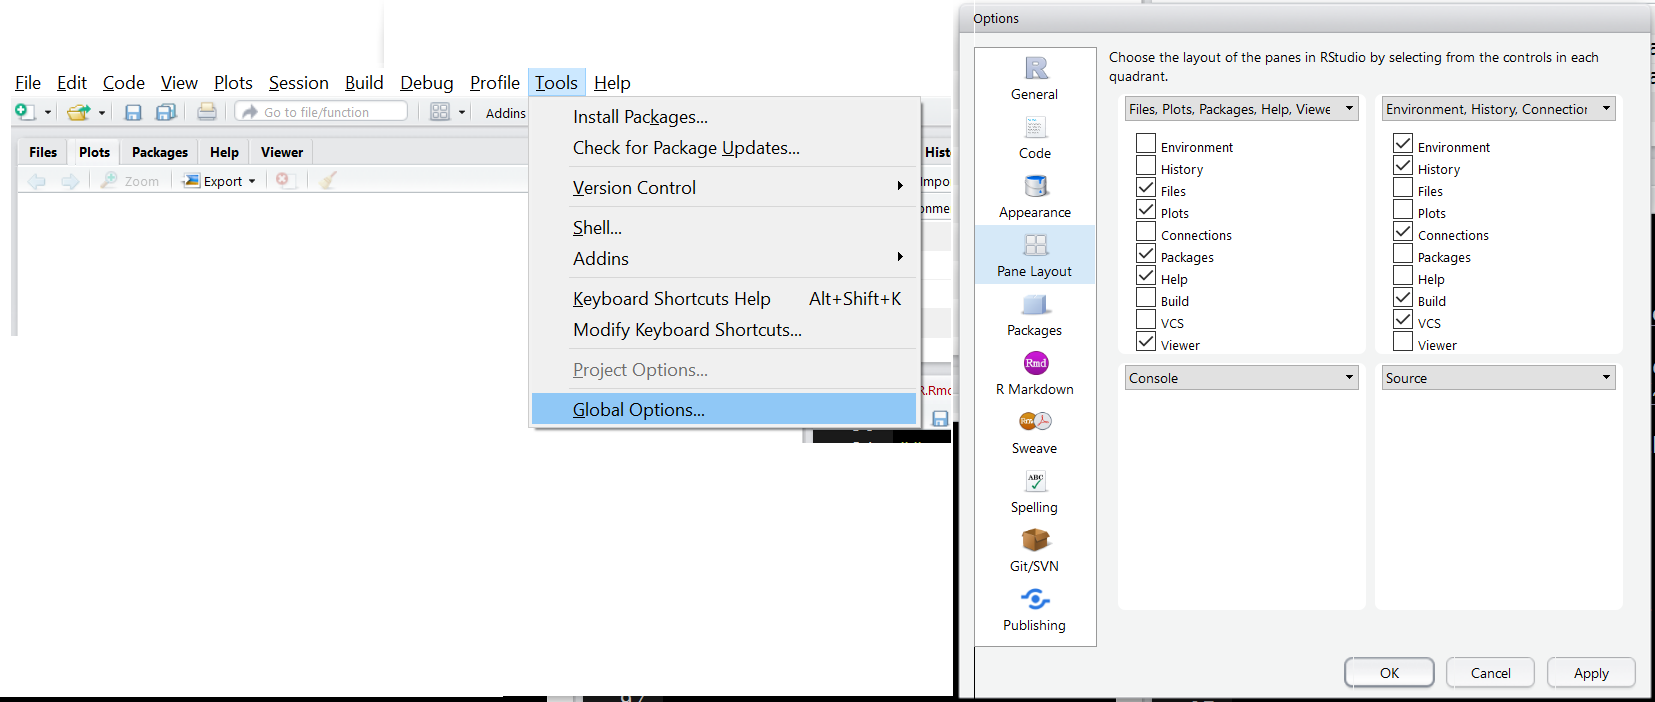
\includegraphics[width=0.8\linewidth]{img/panes}

Other useful global options to change are under the appearance tab (font size, theme) and under the code tab (editing --\textgreater{} soft-wrap, display --\textgreater{} show whitespace).

\hypertarget{console-1}{%
\subsubsection{Console}\label{console-1}}

To evaluate code you can type directly into the \textbf{console}.

\begin{Shaded}
\begin{Highlighting}[]
\CommentTok{#simple math operations}
\CommentTok{# <-- is a comment - code not evaluated}
\DecValTok{3} \OperatorTok{+}\StringTok{ }\DecValTok{7}
\end{Highlighting}
\end{Shaded}

\begin{verbatim}
## [1] 10
\end{verbatim}

\begin{Shaded}
\begin{Highlighting}[]
\DecValTok{10} \OperatorTok{*}\StringTok{ }\KeywordTok{exp}\NormalTok{(}\DecValTok{3}\NormalTok{) }\CommentTok{#exp is exponential function}
\end{Highlighting}
\end{Shaded}

\begin{verbatim}
## [1] 200.8554
\end{verbatim}

\begin{Shaded}
\begin{Highlighting}[]
\KeywordTok{log}\NormalTok{(pi}\OperatorTok{^}\DecValTok{2}\NormalTok{) }\CommentTok{#log is natural log by default}
\end{Highlighting}
\end{Shaded}

\begin{verbatim}
## [1] 2.28946
\end{verbatim}

\begin{Shaded}
\begin{Highlighting}[]
\KeywordTok{mean}\NormalTok{(cars}\OperatorTok{$}\NormalTok{speed)}
\end{Highlighting}
\end{Shaded}

\begin{verbatim}
## [1] 15.4
\end{verbatim}

\begin{Shaded}
\begin{Highlighting}[]
\KeywordTok{hist}\NormalTok{(cars}\OperatorTok{$}\NormalTok{speed)}
\end{Highlighting}
\end{Shaded}

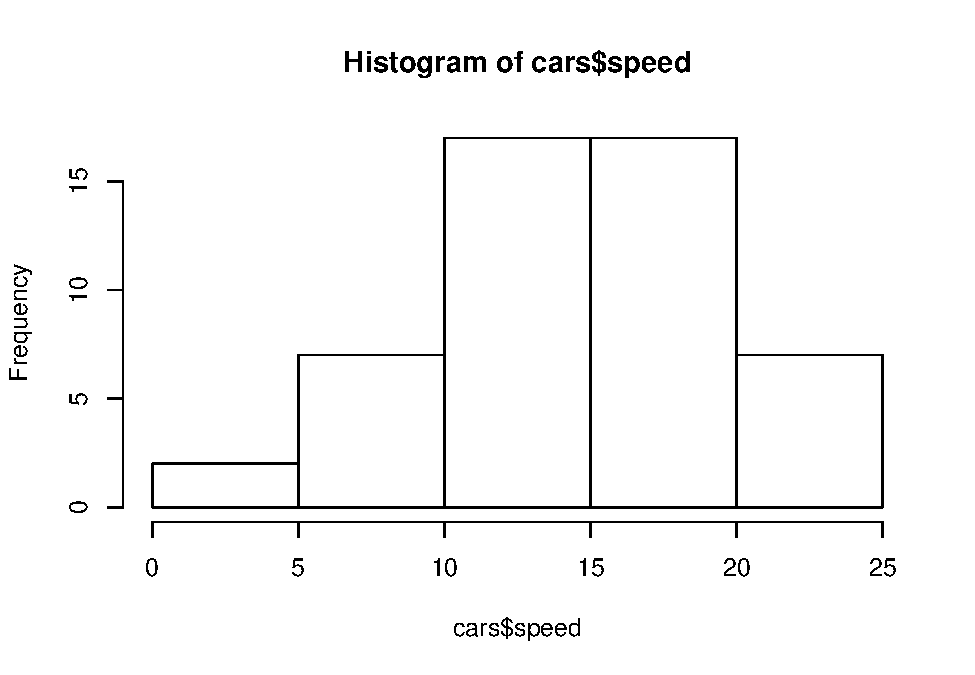
\includegraphics{StatisticalMethods_files/figure-latex/unnamed-chunk-21-1.pdf}

In the R sections of the book we spend much of our time learning the R syntax needed to create the appropriate summaries or analysis.

\hypertarget{scripting-and-viewing-window-1}{%
\subsubsection{Scripting and Viewing Window}\label{scripting-and-viewing-window-1}}

Usually you don't want to type code directly into the console because there isn't an easy way to get the code for later use. Instead code is usually written in an R `script' which is then saved.

From an R script you can send code to console via:

\begin{itemize}
\item
  ``Run'' button (runs current line)
\item
  CTRL+Enter (PC) or Command+Enter (MAC)
\item
  Highlight section and do above
\end{itemize}

To create a new R script you can use the menus at the top and go to File --\textgreater{} New File --\textgreater{} R Script. Take a moment and do this! Type the following into your script:

\begin{itemize}
\item
  \texttt{View(cars)} (note capital \texttt{V})
\item
  \texttt{plot(cars)}
\end{itemize}

Submit it to the console using a button or hot key!

\hypertarget{plotshelp-1}{%
\subsubsection{Plots/Help}\label{plotshelp-1}}

Created plots are stored in the \texttt{Plots} tab. This is a nice feature that allows you to cycle through past plots and easily save plots via menus.

In this pane there is also a \texttt{Help} tab that will enable you to learn about R functions. In the console type \texttt{help(hist)} for instance. Information about the \texttt{hist} function is presented. Being able to parse these types of help files is a really useful skill!

For every R function there are a few sections:

\begin{itemize}
\item
  Description - What the function is intended for.
\item
  Usage - How to call the function, inputs required, and which inputs have default arguments.

  \begin{itemize}
  \tightlist
  \item
    Here we see \texttt{hist(x,\ ...)}. This implies there is only one required input, \texttt{x}, and there is no default.\\
  \item
    Below you see a more detailed call to \texttt{hist} that includes other inputs. Each of these inputs has an equal sign with a value after it. This is the default value for that input (since there is a default value you don't have to specify it when you call). For instance, the \texttt{breaks\ =\ "Sturges"} input implies that the ``Sturges'' method is the default for determining how the bins of the histogram are created.
  \end{itemize}
\item
  Arguments - Describes the input requirements in more detail.
\item
  Details - Information about how the function works.
\item
  Values - Information about what is returned to the user.
\item
  References
\item
  See Also - Related functions.
\item
  Examples - Highly useful section giving code you can copy and paste to see an example of how the function can be used.
\end{itemize}

\hypertarget{environment-1}{%
\subsubsection{Environment}\label{environment-1}}

R stores \textbf{data/info/functions/etc.} in R objects. An object is a data structure having attributes and methods (more on this shortly). You can create an R object via \texttt{\textless{}-} (recommended) or \texttt{=}.

\begin{Shaded}
\begin{Highlighting}[]
\CommentTok{#save for later}
\NormalTok{avg <-}\StringTok{ }\NormalTok{(}\DecValTok{5} \OperatorTok{+}\StringTok{ }\DecValTok{7} \OperatorTok{+}\StringTok{ }\DecValTok{6}\NormalTok{) }\OperatorTok{/}\StringTok{ }\DecValTok{3}
\CommentTok{#call avg object}
\NormalTok{avg}
\end{Highlighting}
\end{Shaded}

\begin{verbatim}
## [1] 6
\end{verbatim}

\begin{Shaded}
\begin{Highlighting}[]
\CommentTok{#strings (text) can be saved as well}
\NormalTok{words <-}\StringTok{ }\KeywordTok{c}\NormalTok{(}\StringTok{"Hello there!"}\NormalTok{, }\StringTok{"How are you?"}\NormalTok{)}
\NormalTok{words}
\end{Highlighting}
\end{Shaded}

\begin{verbatim}
## [1] "Hello there!" "How are you?"
\end{verbatim}

Notice that when you send the line \texttt{avg\ \textless{}-\ (5+\ 7\ +\ 6)\ /\ 3} to the console (i.e.~create the object \texttt{avg}) that nothing prints out. This is common behavior when storing the object. The output or information is saved for later use in the object. To see the output or information you then simply call the object (a default printing method is used to display it).

You can look at all current objects with \texttt{ls()}.

\begin{Shaded}
\begin{Highlighting}[]
\KeywordTok{ls}\NormalTok{()}
\end{Highlighting}
\end{Shaded}

\begin{verbatim}
##  [1] "airquality"    "alpha"         "avg"           "baseURL"      
##  [5] "Batting"       "bodyFatData"   "chicagoData"   "edData"       
##  [9] "fit"           "i"             "index"         "iris"         
## [13] "key"           "lower_bound"   "mat"           "n"            
## [17] "neuralgiaData" "newTempsData"  "phat"          "pihat"        
## [21] "smokeData"     "spellData"     "spellDataDF"   "status"       
## [25] "tb"            "temp"          "tempsData"     "upper_bound"  
## [29] "URL"           "v"             "value"         "vec"          
## [33] "words"         "x"             "y"             "z"
\end{verbatim}

Use \texttt{rm()} to remove an object.

\begin{Shaded}
\begin{Highlighting}[]
\KeywordTok{rm}\NormalTok{(avg)}
\KeywordTok{ls}\NormalTok{()}
\end{Highlighting}
\end{Shaded}

\begin{verbatim}
##  [1] "airquality"    "alpha"         "baseURL"       "Batting"      
##  [5] "bodyFatData"   "chicagoData"   "edData"        "fit"          
##  [9] "i"             "index"         "iris"          "key"          
## [13] "lower_bound"   "mat"           "n"             "neuralgiaData"
## [17] "newTempsData"  "phat"          "pihat"         "smokeData"    
## [21] "spellData"     "spellDataDF"   "status"        "tb"           
## [25] "temp"          "tempsData"     "upper_bound"   "URL"          
## [29] "v"             "value"         "vec"           "words"        
## [33] "x"             "y"             "z"
\end{verbatim}

Built-in objects exist like \texttt{letters} and \texttt{cars}.

\begin{Shaded}
\begin{Highlighting}[]
\NormalTok{letters}
\end{Highlighting}
\end{Shaded}

\begin{verbatim}
##  [1] "a" "b" "c" "d" "e" "f" "g" "h" "i" "j" "k" "l" "m" "n" "o" "p" "q" "r" "s"
## [20] "t" "u" "v" "w" "x" "y" "z"
\end{verbatim}

\begin{Shaded}
\begin{Highlighting}[]
\KeywordTok{head}\NormalTok{(cars, }\DataTypeTok{n =} \DecValTok{3}\NormalTok{)}
\end{Highlighting}
\end{Shaded}

\begin{verbatim}
##   speed dist
## 1     4    2
## 2     4   10
## 3     7    4
\end{verbatim}

The function \texttt{data()} shows available built-in datasets.

You should now be roughly familiar with the four main `areas' of the RStudio IDE:

\begin{itemize}
\item
  Console (\& Terminal)
\item
  Scripting and Viewing Window
\item
  Plots/Help (\& Files/Packages)
\item
  Environment (\& Connections/Git)
\end{itemize}

\hypertarget{r-objects-and-classes-1}{%
\subsection{R Objects and Classes}\label{r-objects-and-classes-1}}

R has strong \textbf{O}bject \textbf{O}riented \textbf{P}rogramming (OOP) tools.

\begin{itemize}
\item
  Object: data structure with attributes (class)
\item
  Method: procedures (functions) that act on object based on attributes
\end{itemize}

R functions like \texttt{print()} or \texttt{plot()} act differently depending on an object's class.

\begin{Shaded}
\begin{Highlighting}[]
\KeywordTok{class}\NormalTok{(cars)}
\end{Highlighting}
\end{Shaded}

\begin{verbatim}
## [1] "data.frame"
\end{verbatim}

\begin{Shaded}
\begin{Highlighting}[]
\KeywordTok{plot}\NormalTok{(cars)}
\end{Highlighting}
\end{Shaded}

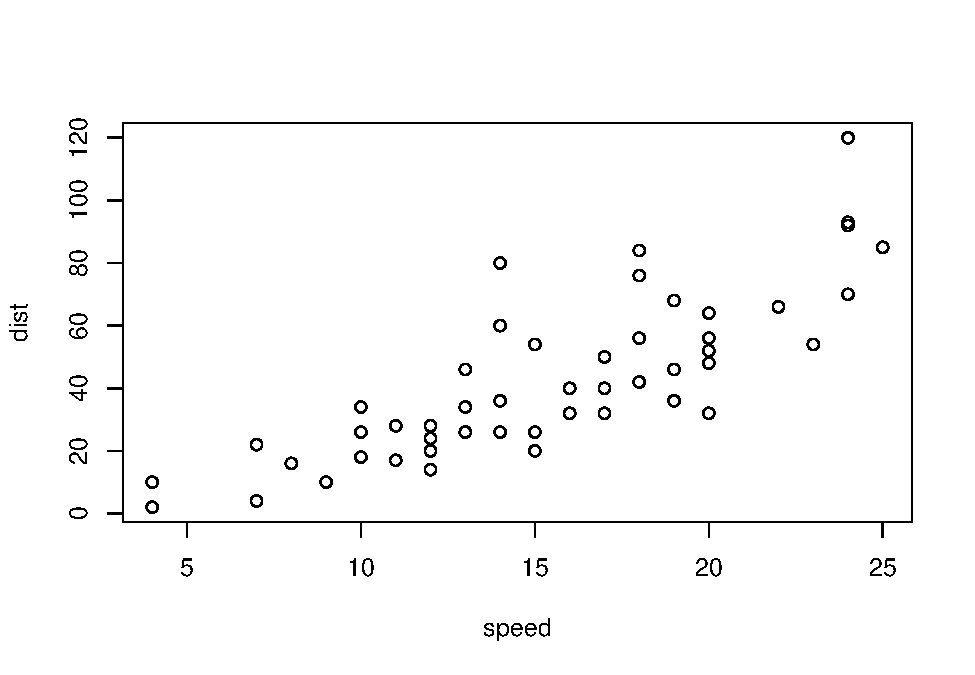
\includegraphics{StatisticalMethods_files/figure-latex/unnamed-chunk-26-1.pdf}

\begin{Shaded}
\begin{Highlighting}[]
\KeywordTok{class}\NormalTok{(exp)}
\end{Highlighting}
\end{Shaded}

\begin{verbatim}
## [1] "function"
\end{verbatim}

\begin{Shaded}
\begin{Highlighting}[]
\KeywordTok{plot}\NormalTok{(exp)}
\end{Highlighting}
\end{Shaded}

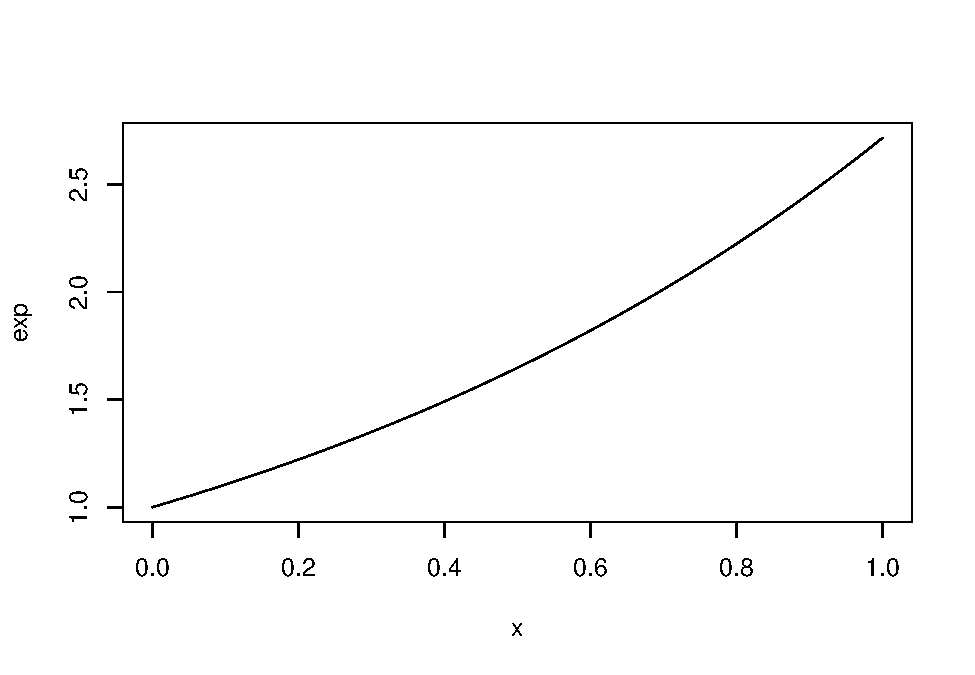
\includegraphics{StatisticalMethods_files/figure-latex/unnamed-chunk-26-2.pdf}

Many R functions exist to help understand an R Object.

\begin{itemize}
\tightlist
\item
  \texttt{str()} (structure)
\end{itemize}

\begin{Shaded}
\begin{Highlighting}[]
\KeywordTok{str}\NormalTok{(cars)}
\end{Highlighting}
\end{Shaded}

\begin{verbatim}
## 'data.frame':    50 obs. of  2 variables:
##  $ speed: num  4 4 7 7 8 9 10 10 10 11 ...
##  $ dist : num  2 10 4 22 16 10 18 26 34 17 ...
\end{verbatim}

\begin{itemize}
\tightlist
\item
  \texttt{class()}
\end{itemize}

\begin{Shaded}
\begin{Highlighting}[]
\KeywordTok{class}\NormalTok{(cars)}
\end{Highlighting}
\end{Shaded}

\begin{verbatim}
## [1] "data.frame"
\end{verbatim}

\begin{itemize}
\tightlist
\item
  \texttt{typeof()}
\end{itemize}

\begin{Shaded}
\begin{Highlighting}[]
\KeywordTok{typeof}\NormalTok{(cars)}
\end{Highlighting}
\end{Shaded}

\begin{verbatim}
## [1] "list"
\end{verbatim}

We'll use these functions later to help us know how to extra information from an R object.

Recall that we can create an R object via \texttt{\textless{}-} (recommended) or \texttt{=}. This allocates computer memory to object. The object's attributes depend on how you created it.

\begin{Shaded}
\begin{Highlighting}[]
\NormalTok{vec <-}\StringTok{ }\KeywordTok{c}\NormalTok{(}\DecValTok{1}\NormalTok{, }\DecValTok{4}\NormalTok{, }\DecValTok{10}\NormalTok{)}
\KeywordTok{class}\NormalTok{(vec)}
\end{Highlighting}
\end{Shaded}

\begin{verbatim}
## [1] "numeric"
\end{verbatim}

\begin{Shaded}
\begin{Highlighting}[]
\NormalTok{fit <-}\StringTok{ }\KeywordTok{lm}\NormalTok{(dist }\OperatorTok{~}\StringTok{ }\NormalTok{speed, }\DataTypeTok{data =}\NormalTok{ cars)}
\KeywordTok{class}\NormalTok{(fit)}
\end{Highlighting}
\end{Shaded}

\begin{verbatim}
## [1] "lm"
\end{verbatim}

\hypertarget{data-objects-1}{%
\subsection{Data Objects}\label{data-objects-1}}

To understand how to use R for data analysis we need to understand commonly used data structures:

\begin{verbatim}
 1. Atomic Vector (1D)  
 2. Matrix (2D)  
 3. Array (nd) (not covered)  
 4. Data Frame (2D)  
 5. List (1D)  
\end{verbatim}

\hypertarget{atomic-vector-1}{%
\subsubsection{Atomic Vector}\label{atomic-vector-1}}

Let's start with the most basic object and work our way up. An atomic vector is a 1D group of elements with an ordering.

\begin{center}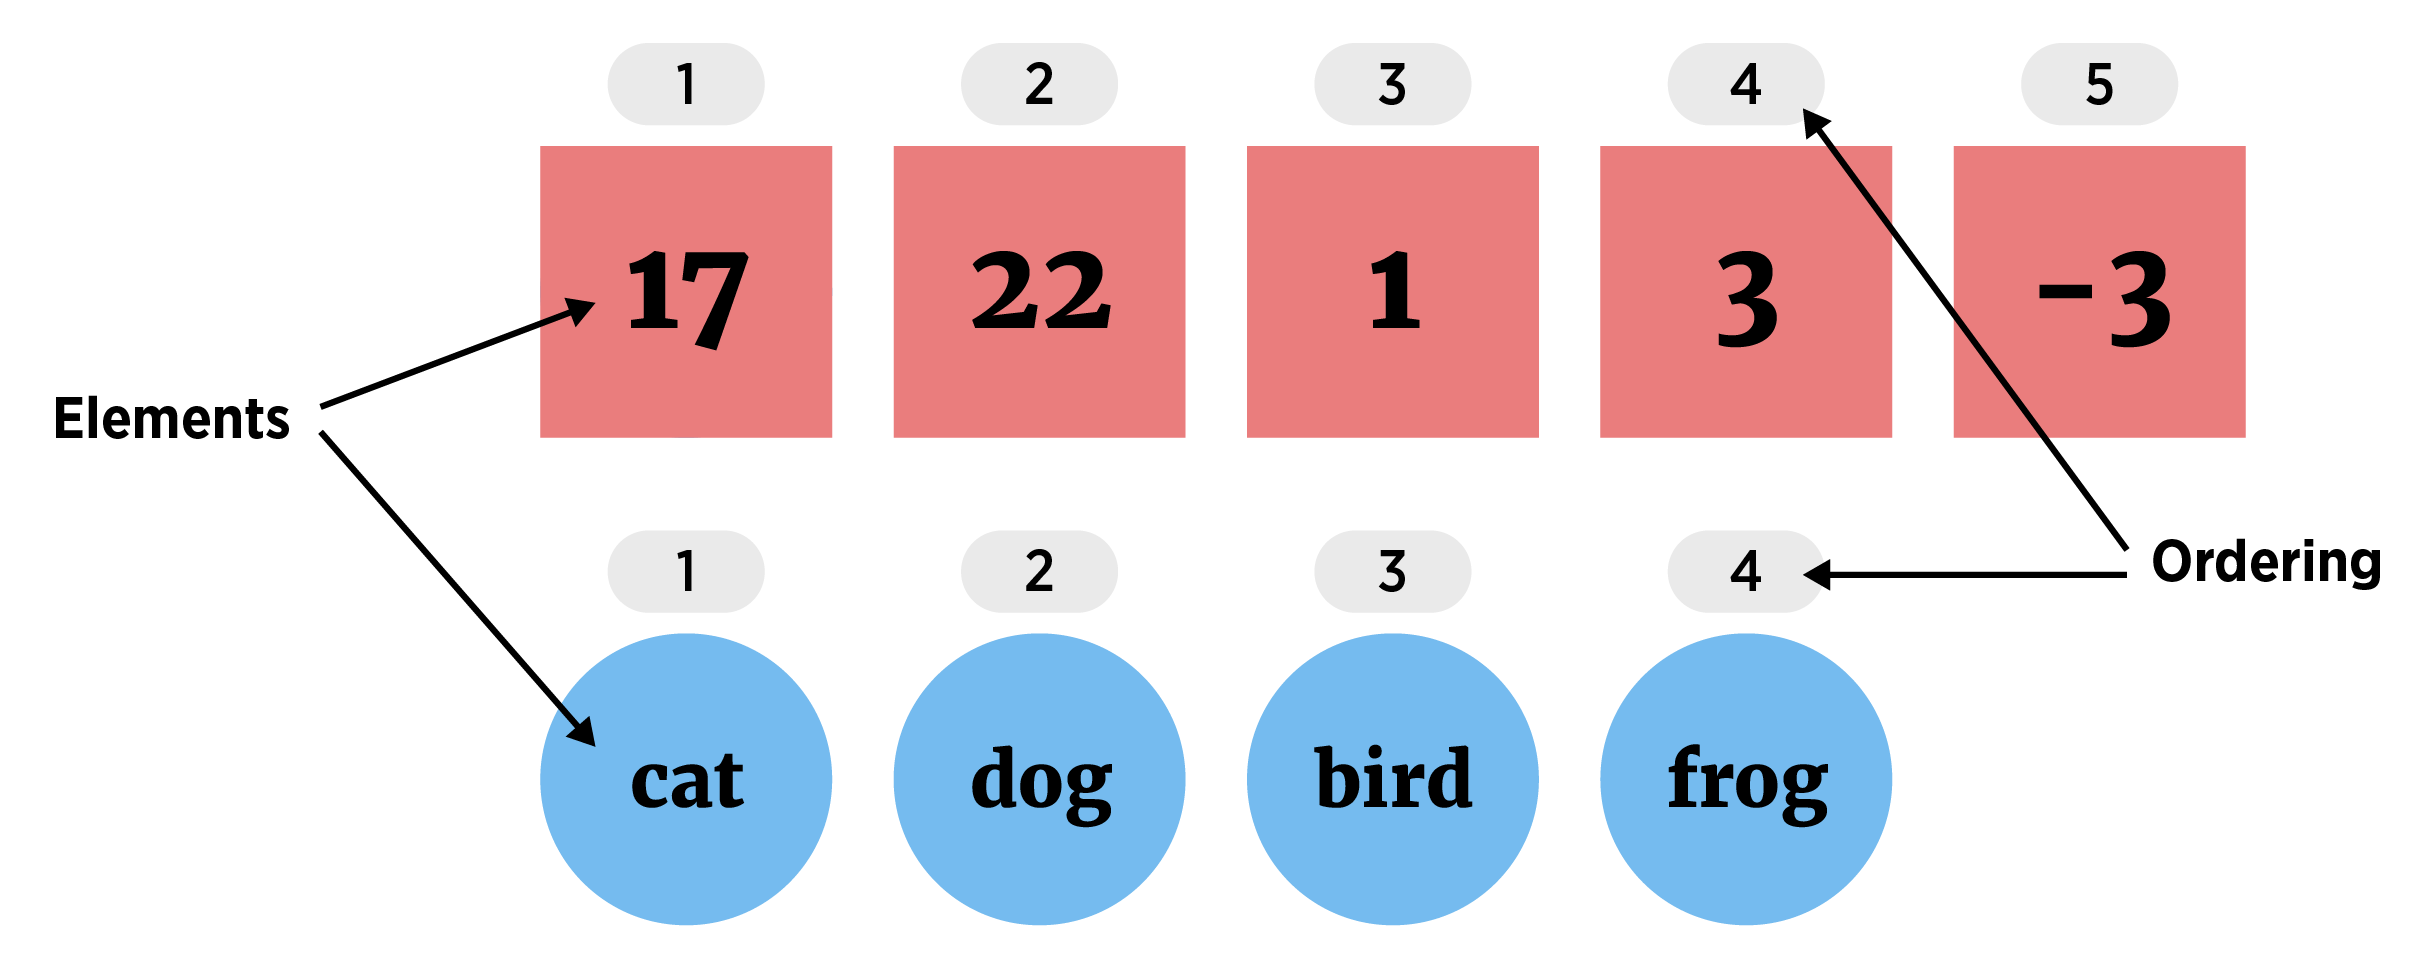
\includegraphics[width=0.8\linewidth]{img/vectorVisualF} \end{center}

All of the elements must be same `type'. Types include numeric (integer or double), character, or logical. We create an atomic vector with the \texttt{c()} function (`combine').

\begin{Shaded}
\begin{Highlighting}[]
\CommentTok{#vectors (1 dimensional) objects}
\NormalTok{x <-}\StringTok{ }\KeywordTok{c}\NormalTok{(}\DecValTok{17}\NormalTok{, }\DecValTok{22}\NormalTok{, }\DecValTok{1}\NormalTok{, }\DecValTok{3}\NormalTok{, }\DecValTok{-3}\NormalTok{)}
\NormalTok{y <-}\StringTok{ }\KeywordTok{c}\NormalTok{(}\StringTok{"cat"}\NormalTok{, }\StringTok{"dog"}\NormalTok{, }\StringTok{"bird"}\NormalTok{, }\StringTok{"frog"}\NormalTok{)}
\NormalTok{x}
\end{Highlighting}
\end{Shaded}

\begin{verbatim}
## [1] 17 22  1  3 -3
\end{verbatim}

\begin{Shaded}
\begin{Highlighting}[]
\NormalTok{y}
\end{Highlighting}
\end{Shaded}

\begin{verbatim}
## [1] "cat"  "dog"  "bird" "frog"
\end{verbatim}

In addition, many `functions' output a numeric vector. Functions are at the heart of R so it is vital to understand them. The concept of a function is that there the function takes an input or inputs and maps those inputs to some output(s).

\begin{center}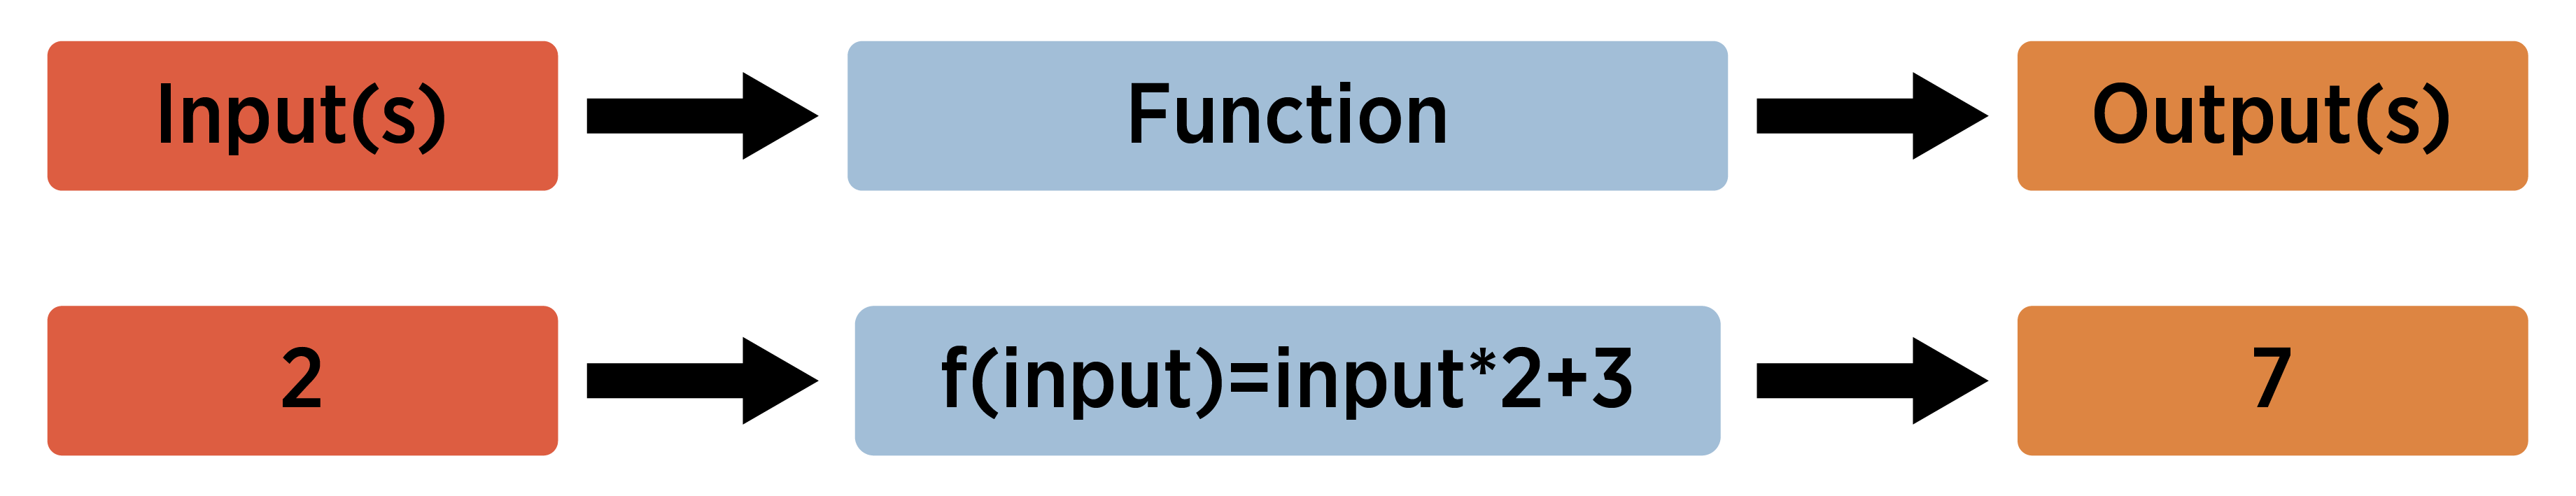
\includegraphics[width=0.8\linewidth]{img/funVisual1F} \end{center}

As an example, one function that outputs a numeric vector is the \texttt{seq} or sequence function. To know about a function you need to know about the inputs and ouputs. For \texttt{seq} we have the following:

\begin{verbatim}
+ Inputs = from, to, by (among others)  

+ Output = a sequence of numbers
\end{verbatim}

\begin{center}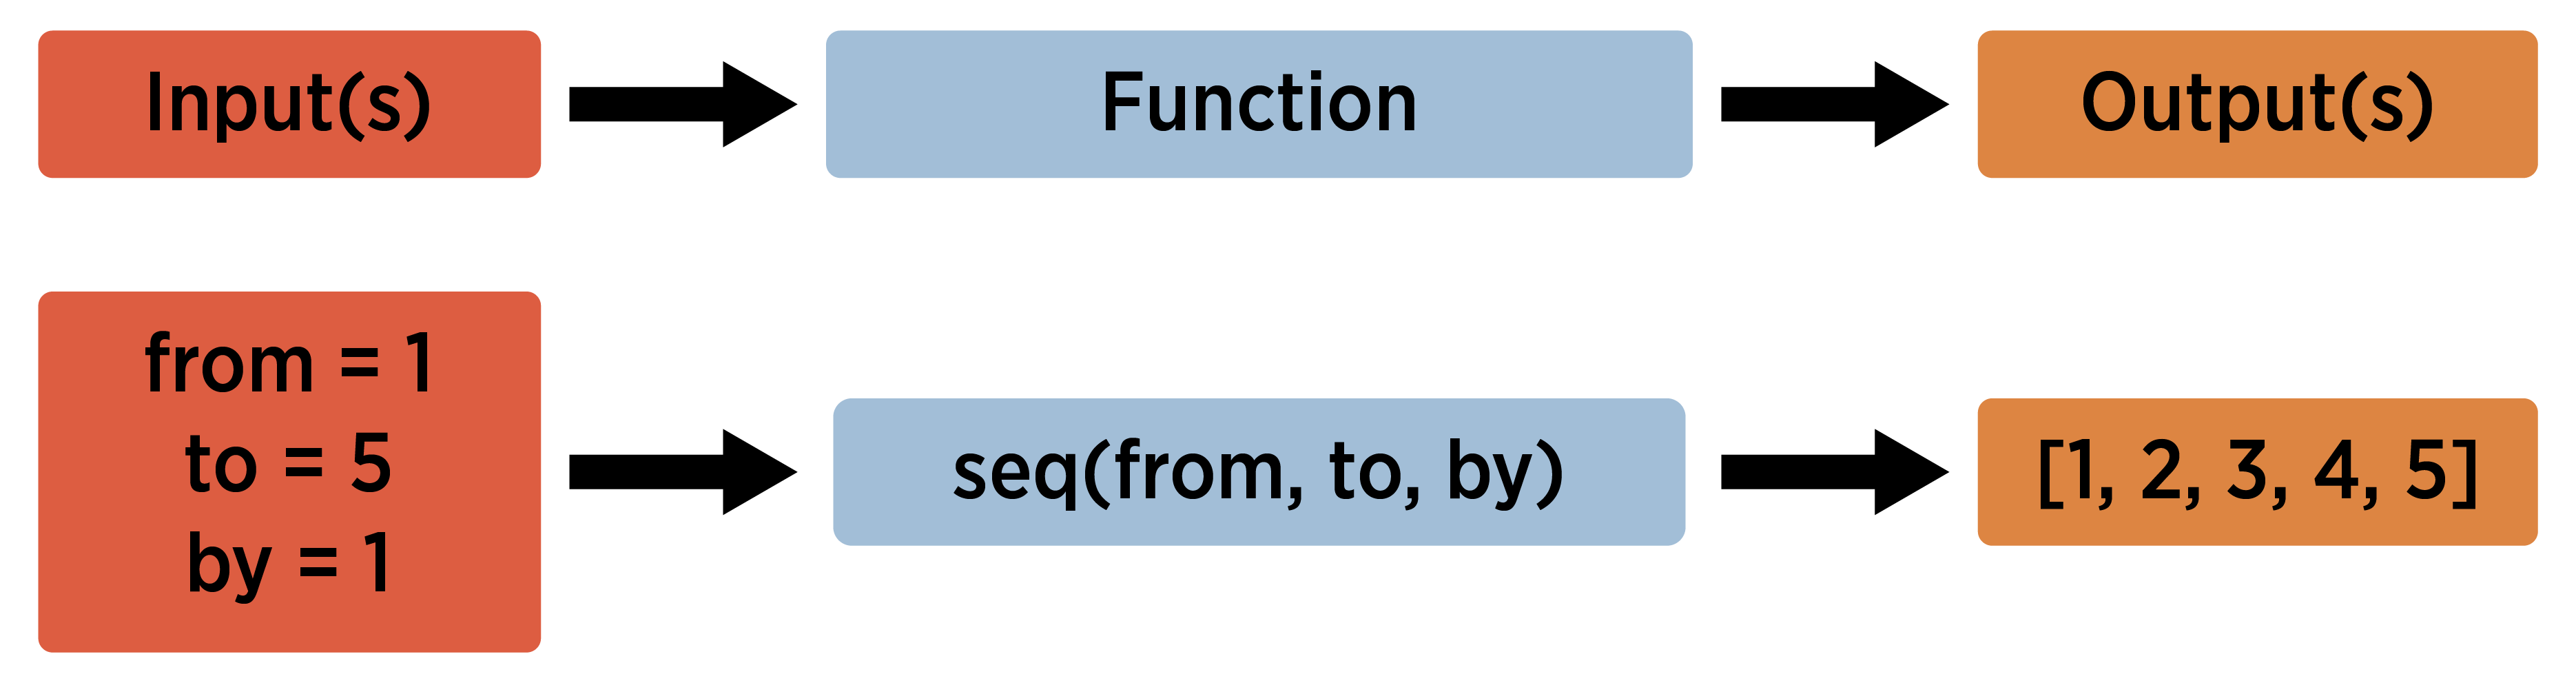
\includegraphics[width=0.8\linewidth]{img/funVisual2F} \end{center}

\begin{Shaded}
\begin{Highlighting}[]
\NormalTok{v <-}\StringTok{ }\KeywordTok{seq}\NormalTok{(}\DataTypeTok{from =} \DecValTok{1}\NormalTok{, }\DataTypeTok{to =} \DecValTok{5}\NormalTok{, }\DataTypeTok{by =} \DecValTok{1}\NormalTok{)}
\NormalTok{v}
\end{Highlighting}
\end{Shaded}

\begin{verbatim}
## [1] 1 2 3 4 5
\end{verbatim}

\begin{Shaded}
\begin{Highlighting}[]
\KeywordTok{str}\NormalTok{(v)}
\end{Highlighting}
\end{Shaded}

\begin{verbatim}
##  num [1:5] 1 2 3 4 5
\end{verbatim}

\texttt{str} tells about the object \texttt{v}:

\begin{itemize}
\item
  \texttt{num} says it is numeric
\item
  \texttt{{[}1:5{]}} implies one dimensional with elements 1, 2, 3, 4, 5
\end{itemize}

The \texttt{seq} function is used quite a bit. There is a shorthand way to create an integer sequence using \texttt{:}.

\begin{Shaded}
\begin{Highlighting}[]
\DecValTok{1}\OperatorTok{:}\DecValTok{20} 
\end{Highlighting}
\end{Shaded}

\begin{verbatim}
##  [1]  1  2  3  4  5  6  7  8  9 10 11 12 13 14 15 16 17 18 19 20
\end{verbatim}

It is also important to know how R does math on its objects. R does elementwise addition/subtraction and multiplication/division to vectors, matrices, and data frames. (The matrix multiplicaiton operator is \texttt{\%*\%}.).

\begin{Shaded}
\begin{Highlighting}[]
\DecValTok{1}\OperatorTok{:}\DecValTok{20}\OperatorTok{/}\DecValTok{20}
\end{Highlighting}
\end{Shaded}

\begin{verbatim}
##  [1] 0.05 0.10 0.15 0.20 0.25 0.30 0.35 0.40 0.45 0.50 0.55 0.60 0.65 0.70 0.75
## [16] 0.80 0.85 0.90 0.95 1.00
\end{verbatim}

\begin{Shaded}
\begin{Highlighting}[]
\DecValTok{1}\OperatorTok{:}\DecValTok{20} \OperatorTok{+}\StringTok{ }\DecValTok{1}
\end{Highlighting}
\end{Shaded}

\begin{verbatim}
##  [1]  2  3  4  5  6  7  8  9 10 11 12 13 14 15 16 17 18 19 20 21
\end{verbatim}

As we mentioned earlier, understanding help files is really useful to being about to program in R. As functions are ubiquitous in R we often need to learn about their inputs (or arguments) and we can do so using \texttt{help}.

To recap, our first commonly used R object for storing data is an atomic vectore. This is a 1D group of elements with an ordering where all of the elements are of the same type. Generally vectors are useful to know about but not usually useful for a storing a dataset exactly. They can often be considered as the `building blocks' for other data types.

\hypertarget{matrix-1}{%
\subsubsection{Matrix}\label{matrix-1}}

A Matrix is a 2D data structure in R whose elements are all of the same type. The first dimension refers to the rows and the second dimension refers to the columns. A 2D data object is very common. The rows often represent the \emph{observations} and the columns represent the \emph{variables}. Although not technically right, it is useful to think of the columns of a matrix as vectors of the same \textbf{type and length}.

\begin{center}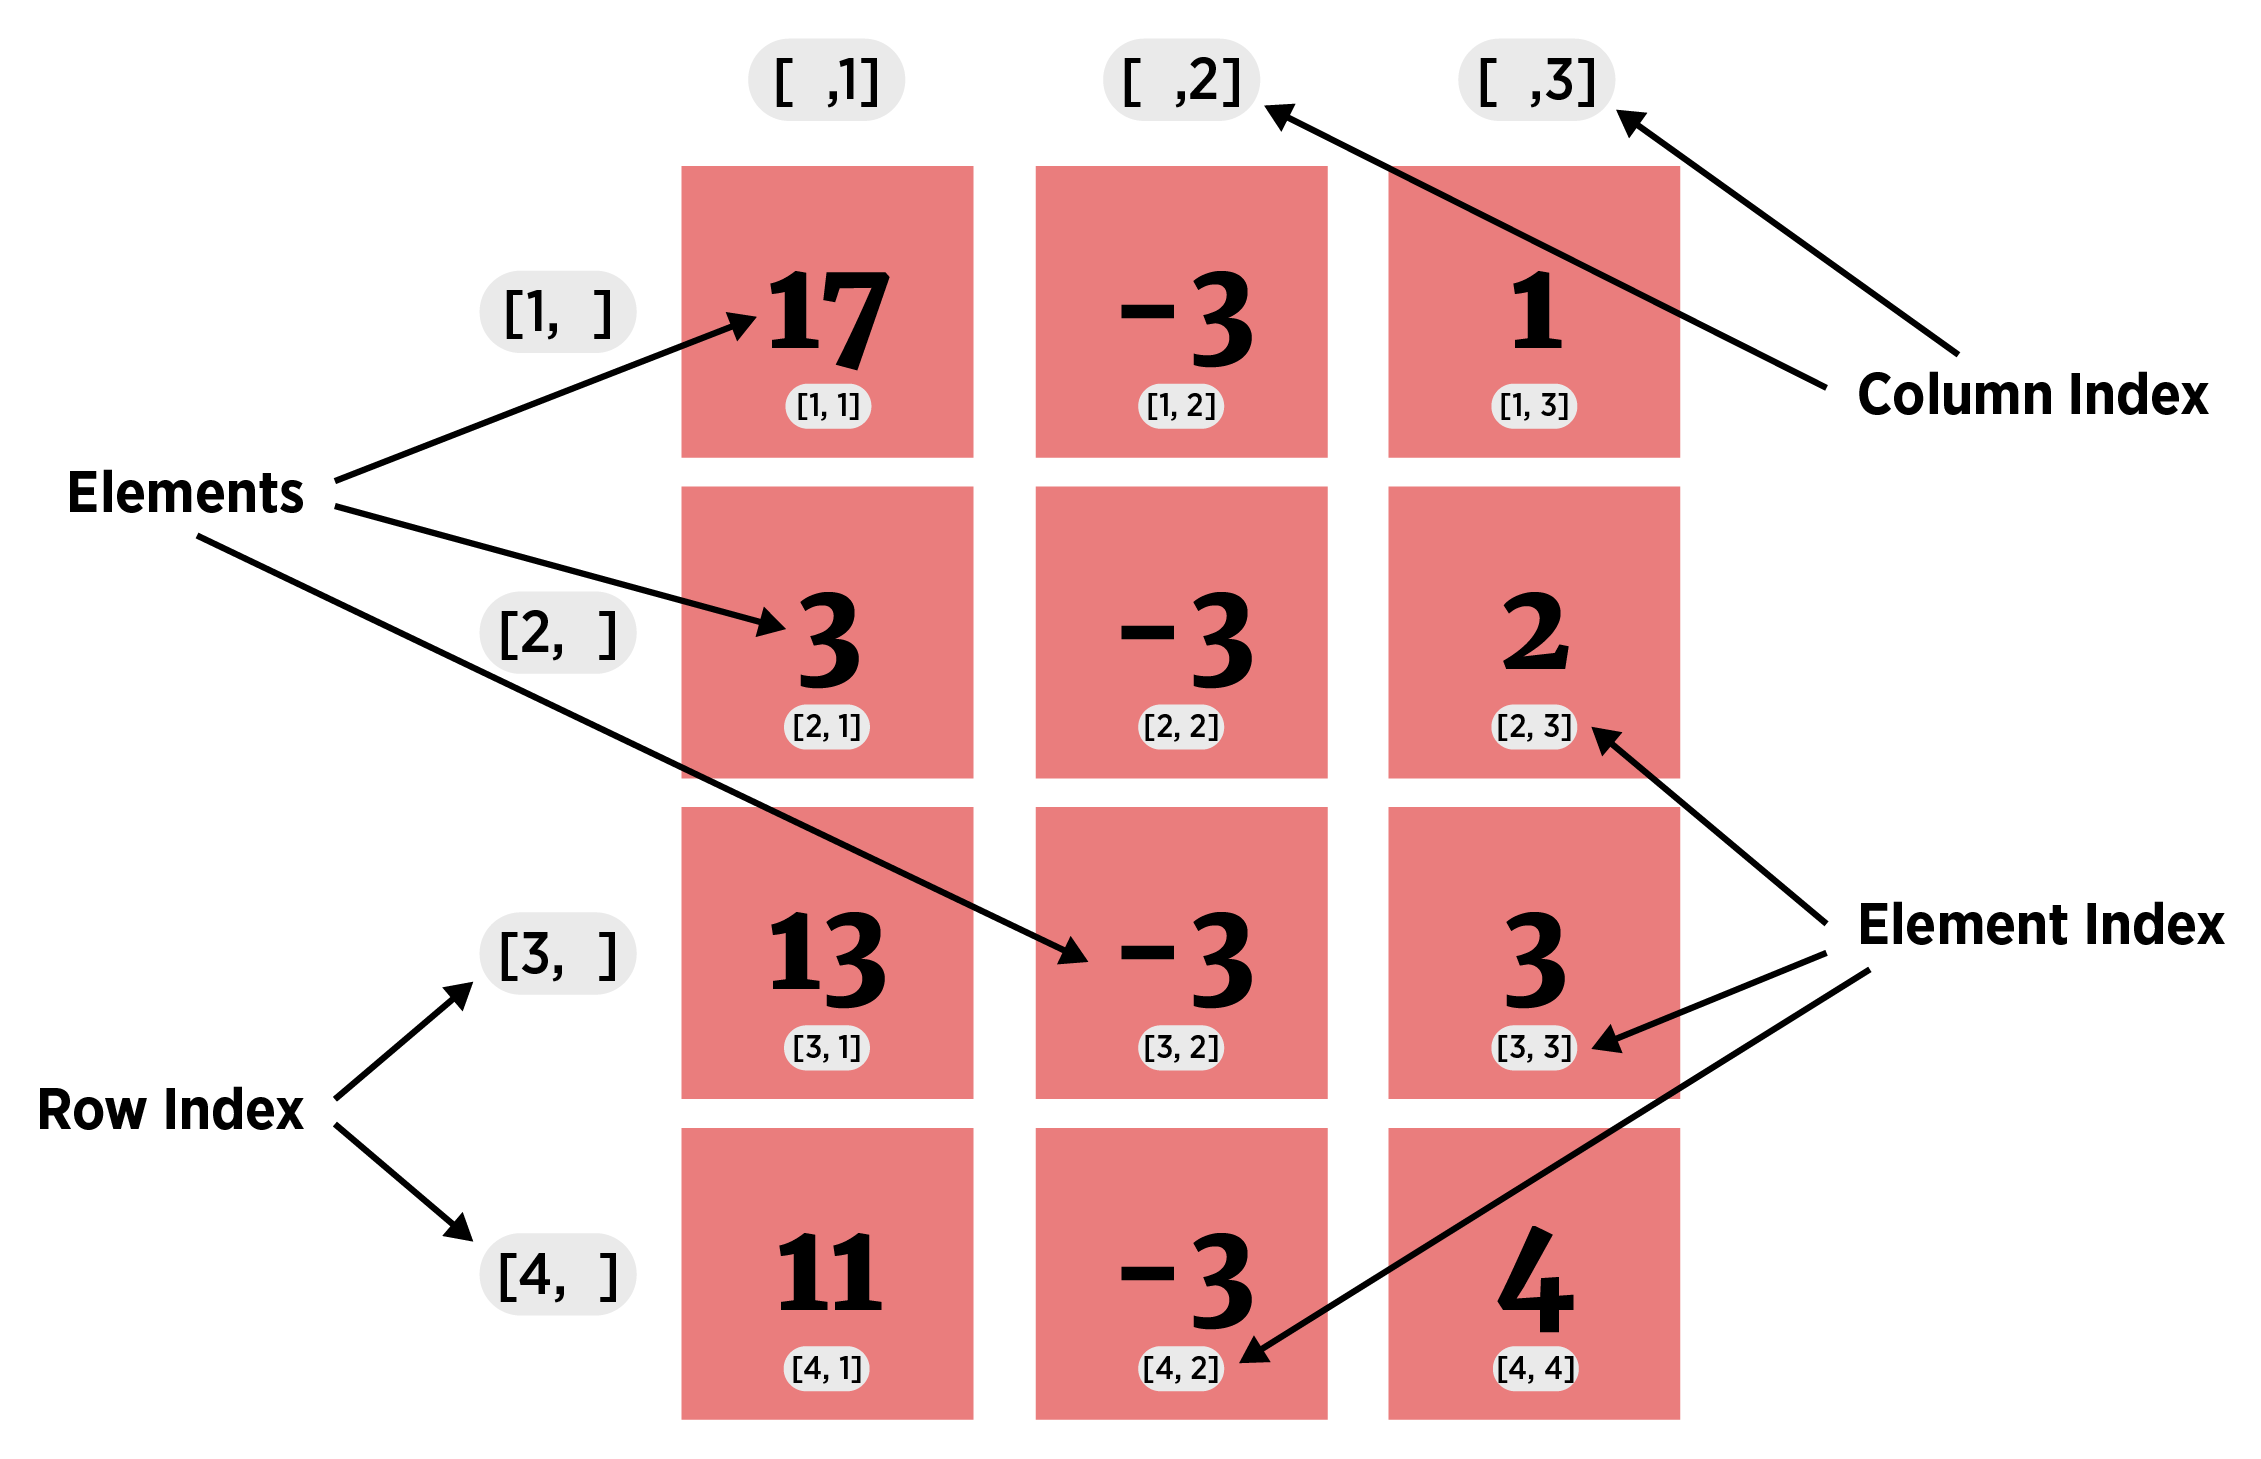
\includegraphics[width=0.75\linewidth]{img/matrixVisualF} \end{center}

For instance, consider the three vectors created here:

\begin{Shaded}
\begin{Highlighting}[]
\CommentTok{#populate vectors}
\NormalTok{x <-}\StringTok{ }\KeywordTok{c}\NormalTok{(}\DecValTok{17}\NormalTok{, }\DecValTok{3}\NormalTok{, }\DecValTok{13}\NormalTok{, }\DecValTok{11}\NormalTok{)}
\NormalTok{y <-}\StringTok{ }\KeywordTok{rep}\NormalTok{(}\OperatorTok{-}\DecValTok{3}\NormalTok{, }\DataTypeTok{times =} \DecValTok{4}\NormalTok{)}
\NormalTok{z <-}\StringTok{ }\DecValTok{1}\OperatorTok{:}\DecValTok{4}
\end{Highlighting}
\end{Shaded}

These are all of the same type. This can be checked with an \texttt{is.} (read as `is dot') function.

\begin{Shaded}
\begin{Highlighting}[]
\CommentTok{#check 'type'}
\KeywordTok{is.numeric}\NormalTok{(x)}
\end{Highlighting}
\end{Shaded}

\begin{verbatim}
## [1] TRUE
\end{verbatim}

\begin{Shaded}
\begin{Highlighting}[]
\KeywordTok{is.numeric}\NormalTok{(y)}
\end{Highlighting}
\end{Shaded}

\begin{verbatim}
## [1] TRUE
\end{verbatim}

\begin{Shaded}
\begin{Highlighting}[]
\KeywordTok{is.numeric}\NormalTok{(z)}
\end{Highlighting}
\end{Shaded}

\begin{verbatim}
## [1] TRUE
\end{verbatim}

Not only are these three objects the same type but they are also the same length. This can be checked using the \texttt{length} function.

\begin{Shaded}
\begin{Highlighting}[]
\CommentTok{#check 'length'}
\KeywordTok{length}\NormalTok{(x)}
\end{Highlighting}
\end{Shaded}

\begin{verbatim}
## [1] 4
\end{verbatim}

\begin{Shaded}
\begin{Highlighting}[]
\KeywordTok{length}\NormalTok{(y)}
\end{Highlighting}
\end{Shaded}

\begin{verbatim}
## [1] 4
\end{verbatim}

\begin{Shaded}
\begin{Highlighting}[]
\KeywordTok{length}\NormalTok{(z)}
\end{Highlighting}
\end{Shaded}

\begin{verbatim}
## [1] 4
\end{verbatim}

Again, it is useful to visualize the columns of a potential matrix as these vectors. We can create the matrix using the \texttt{matrix} function. The \texttt{matrix} function requires us to give the data as one vector. We can combine the \texttt{x}, \texttt{y}, and \texttt{z} objects into one vector using the \texttt{c} funciton. This is the first argument to the \texttt{matrix} function. The only other argument required is to either specify the number of rows (\texttt{nrow\ =}) or the number of columns (\texttt{ncol\ =}) (R will attempt to figure out the one that is not given using the total length of the specified data vector).

\begin{Shaded}
\begin{Highlighting}[]
\CommentTok{#combine in a matrix}
\KeywordTok{matrix}\NormalTok{(}\KeywordTok{c}\NormalTok{(x, y, z), }\DataTypeTok{ncol =} \DecValTok{3}\NormalTok{)}
\end{Highlighting}
\end{Shaded}

\begin{verbatim}
##      [,1] [,2] [,3]
## [1,]   17   -3    1
## [2,]    3   -3    2
## [3,]   13   -3    3
## [4,]   11   -3    4
\end{verbatim}

A matrix can also store character data as well. An example of this is given below and the number of rows is specified rather than the number of columns. Note the use of \texttt{is.character} from the \texttt{is.} family of functions.

\begin{Shaded}
\begin{Highlighting}[]
\NormalTok{x <-}\StringTok{ }\KeywordTok{c}\NormalTok{(}\StringTok{"Hi"}\NormalTok{, }\StringTok{"There"}\NormalTok{, }\StringTok{"!"}\NormalTok{)}
\NormalTok{y <-}\StringTok{ }\KeywordTok{c}\NormalTok{(}\StringTok{"a"}\NormalTok{, }\StringTok{"b"}\NormalTok{, }\StringTok{"c"}\NormalTok{)}
\NormalTok{z <-}\StringTok{ }\KeywordTok{c}\NormalTok{(}\StringTok{"One"}\NormalTok{, }\StringTok{"Two"}\NormalTok{, }\StringTok{"Three"}\NormalTok{)}
\KeywordTok{is.character}\NormalTok{(x)}
\end{Highlighting}
\end{Shaded}

\begin{verbatim}
## [1] TRUE
\end{verbatim}

\begin{Shaded}
\begin{Highlighting}[]
\KeywordTok{matrix}\NormalTok{(}\KeywordTok{c}\NormalTok{(x, y, z), }\DataTypeTok{nrow =} \DecValTok{3}\NormalTok{)}
\end{Highlighting}
\end{Shaded}

\begin{verbatim}
##      [,1]    [,2] [,3]   
## [1,] "Hi"    "a"  "One"  
## [2,] "There" "b"  "Two"  
## [3,] "!"     "c"  "Three"
\end{verbatim}

To recap, a Matrix is a 2D data structure where we can think of the columns as vectors of the same \textbf{type and length}. These are useful for some datasets but most datasets have some numeric and some character variables.

\begin{center}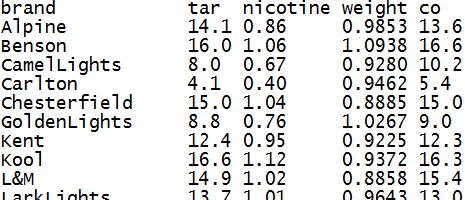
\includegraphics[width=0.8\linewidth]{img/dataset} \end{center}

Another 2D object called a data frame is perfect for this type of data!

\hypertarget{data-frame-1}{%
\subsubsection{Data Frame}\label{data-frame-1}}

A Data Frame is a 2D data structure where elements within a column must be of the same type but the columns themselves can differ in type. When thinking of a data frame, consider them as a collection (list) of vectors of the same \textbf{length}.

\begin{center}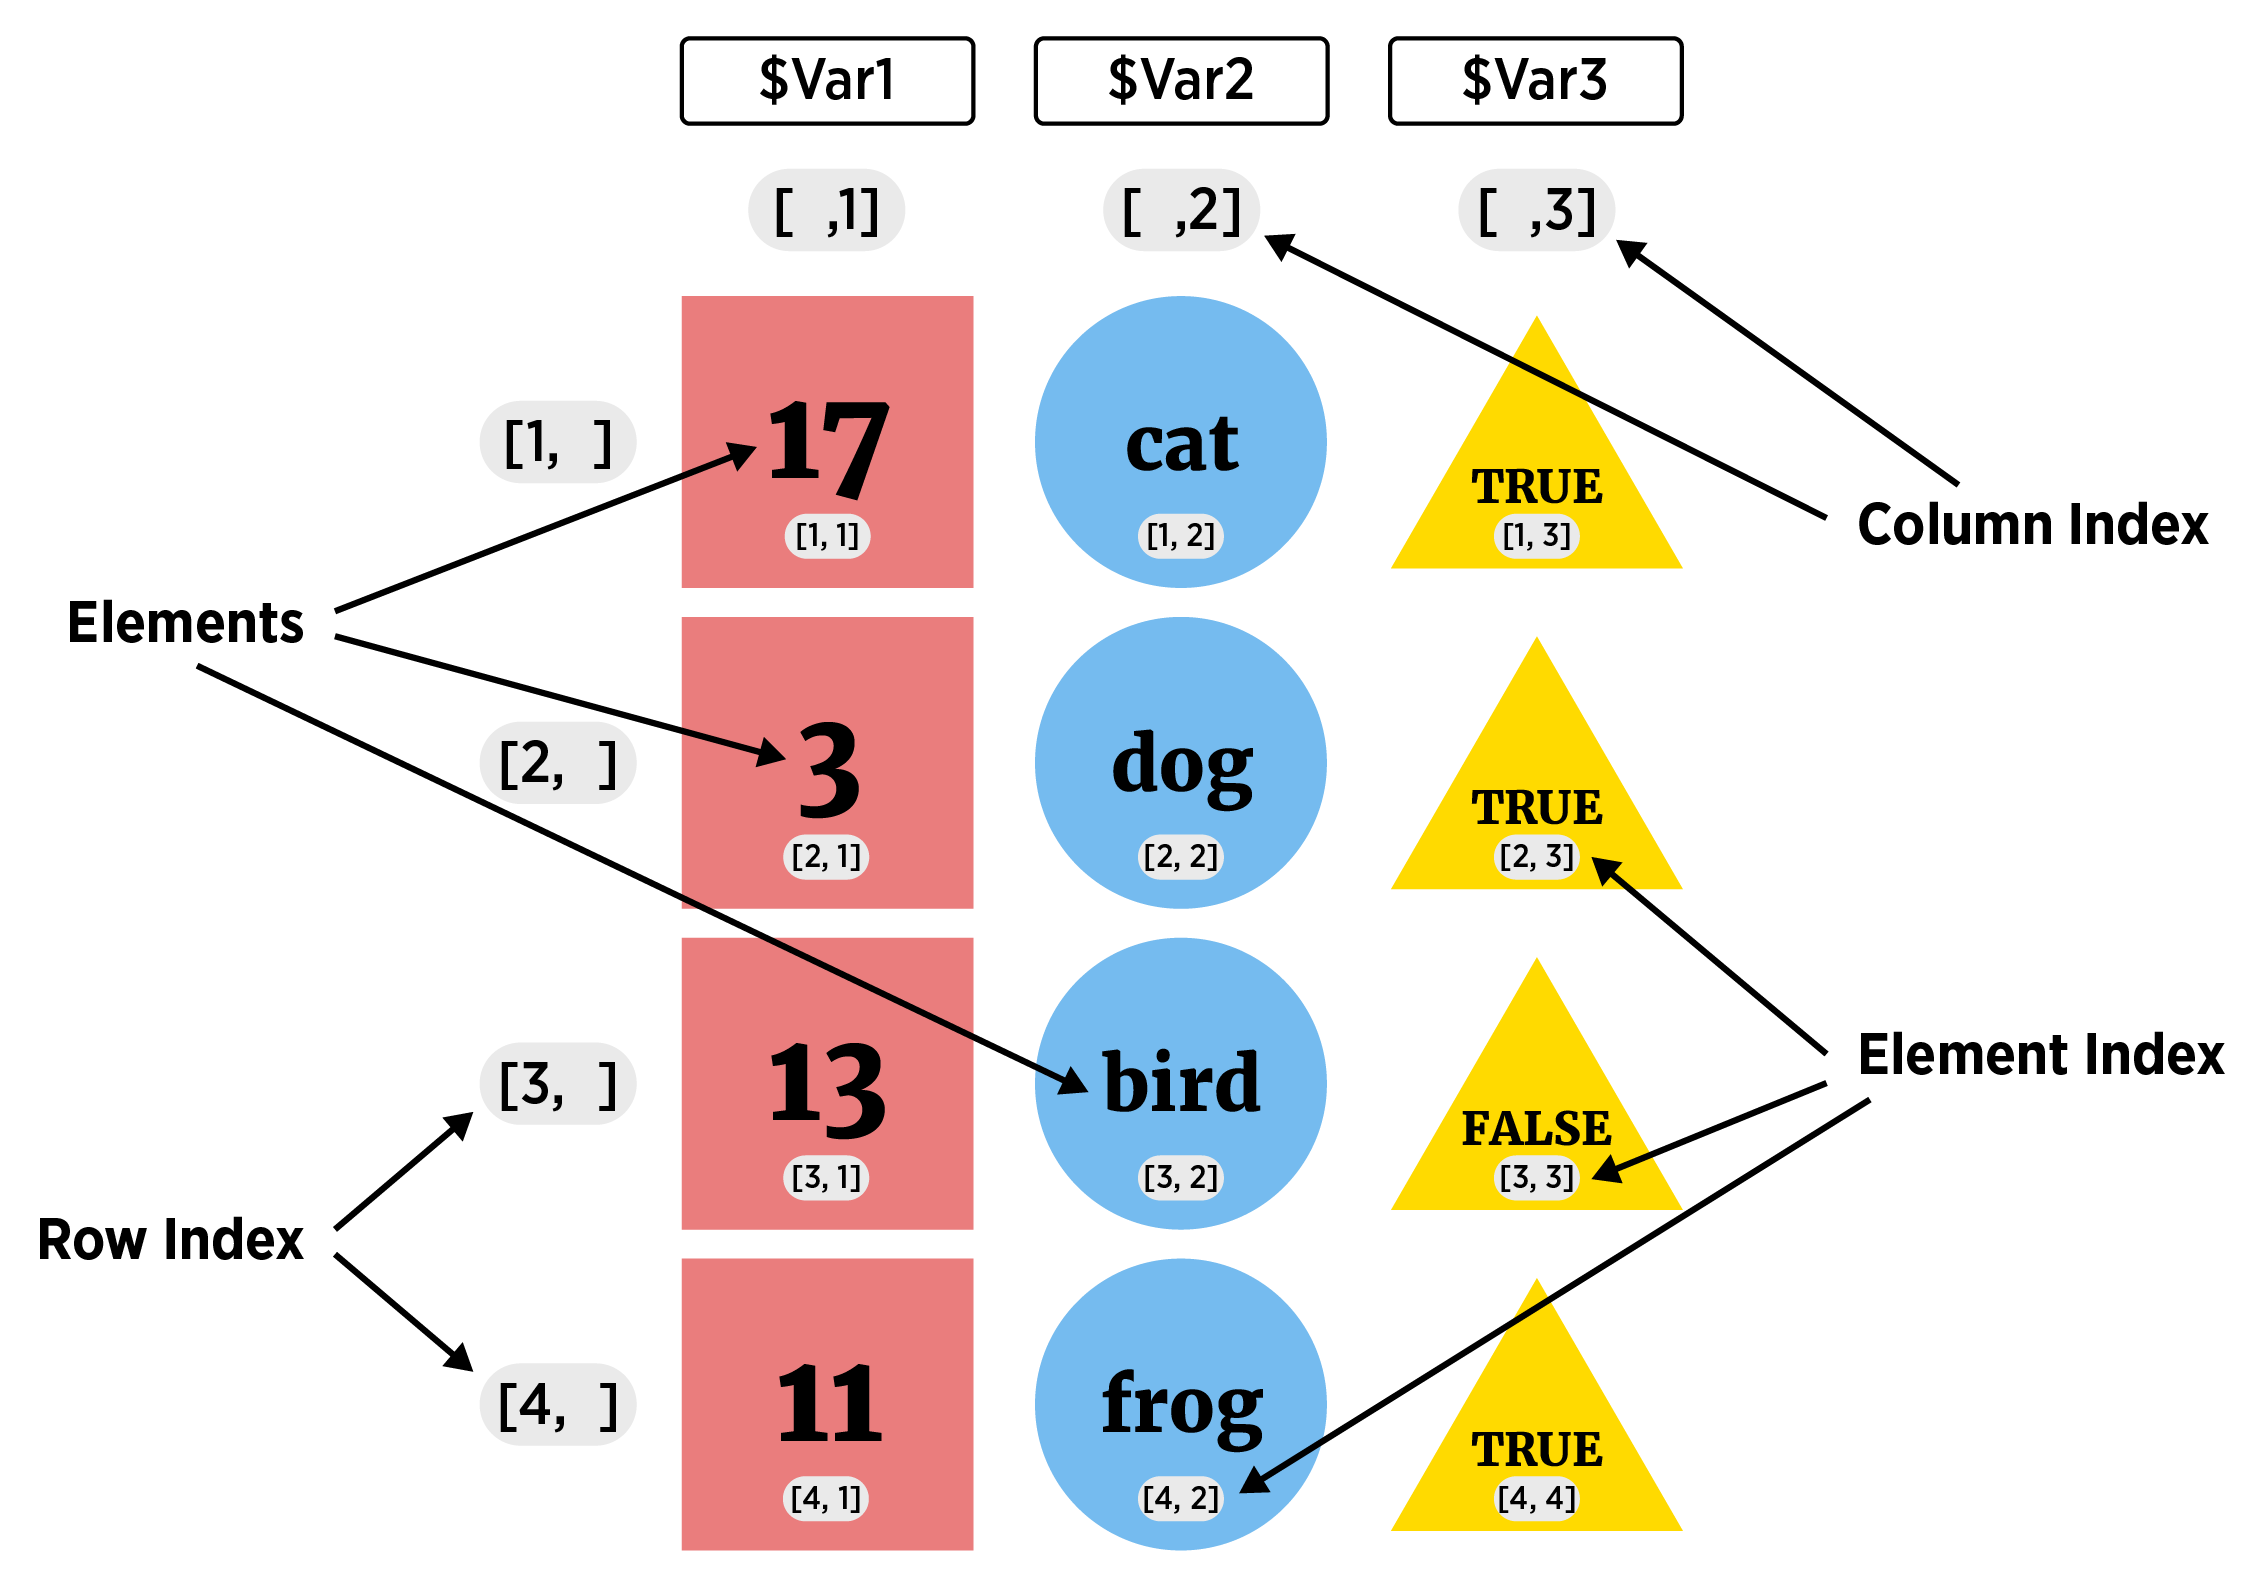
\includegraphics[width=0.8\linewidth]{img/dfVisualF} \end{center}

A data frame can be created with the \texttt{data.frame} function.

\begin{Shaded}
\begin{Highlighting}[]
\NormalTok{x <-}\StringTok{ }\KeywordTok{c}\NormalTok{(}\StringTok{"a"}\NormalTok{, }\StringTok{"b"}\NormalTok{, }\StringTok{"c"}\NormalTok{, }\StringTok{"d"}\NormalTok{, }\StringTok{"e"}\NormalTok{, }\StringTok{"f"}\NormalTok{)}
\NormalTok{y <-}\StringTok{ }\KeywordTok{c}\NormalTok{(}\DecValTok{1}\NormalTok{, }\DecValTok{3}\NormalTok{, }\DecValTok{4}\NormalTok{, }\DecValTok{-1}\NormalTok{, }\DecValTok{5}\NormalTok{, }\DecValTok{6}\NormalTok{)}
\NormalTok{z <-}\StringTok{ }\DecValTok{10}\OperatorTok{:}\DecValTok{15}
\KeywordTok{data.frame}\NormalTok{(x, y, z)}
\end{Highlighting}
\end{Shaded}

\begin{verbatim}
##   x  y  z
## 1 a  1 10
## 2 b  3 11
## 3 c  4 12
## 4 d -1 13
## 5 e  5 14
## 6 f  6 15
\end{verbatim}

You can also easily name the columns during creation.

\begin{Shaded}
\begin{Highlighting}[]
\KeywordTok{data.frame}\NormalTok{(}\DataTypeTok{char =}\NormalTok{ x, }\DataTypeTok{data1 =}\NormalTok{ y, }\DataTypeTok{data2 =}\NormalTok{ z)}
\end{Highlighting}
\end{Shaded}

\begin{verbatim}
##   char data1 data2
## 1    a     1    10
## 2    b     3    11
## 3    c     4    12
## 4    d    -1    13
## 5    e     5    14
## 6    f     6    15
\end{verbatim}

Notice that char, data1, and data2 become the variable names for the data frame.

To recap, consider a data frame as a collection (list) of vectors of the same \textbf{length}. Tis type of data structure is perfect for most data sets! Most functions that read 2D data into R store it as a data frame.

\hypertarget{list-1}{%
\subsubsection{List}\label{list-1}}

A List is a 1D group of objects with ordering. Really it is a vector that can have differing elements. Think of this in a similar way to the atomic vector previously discussed except the elements are really flexible.

\begin{center}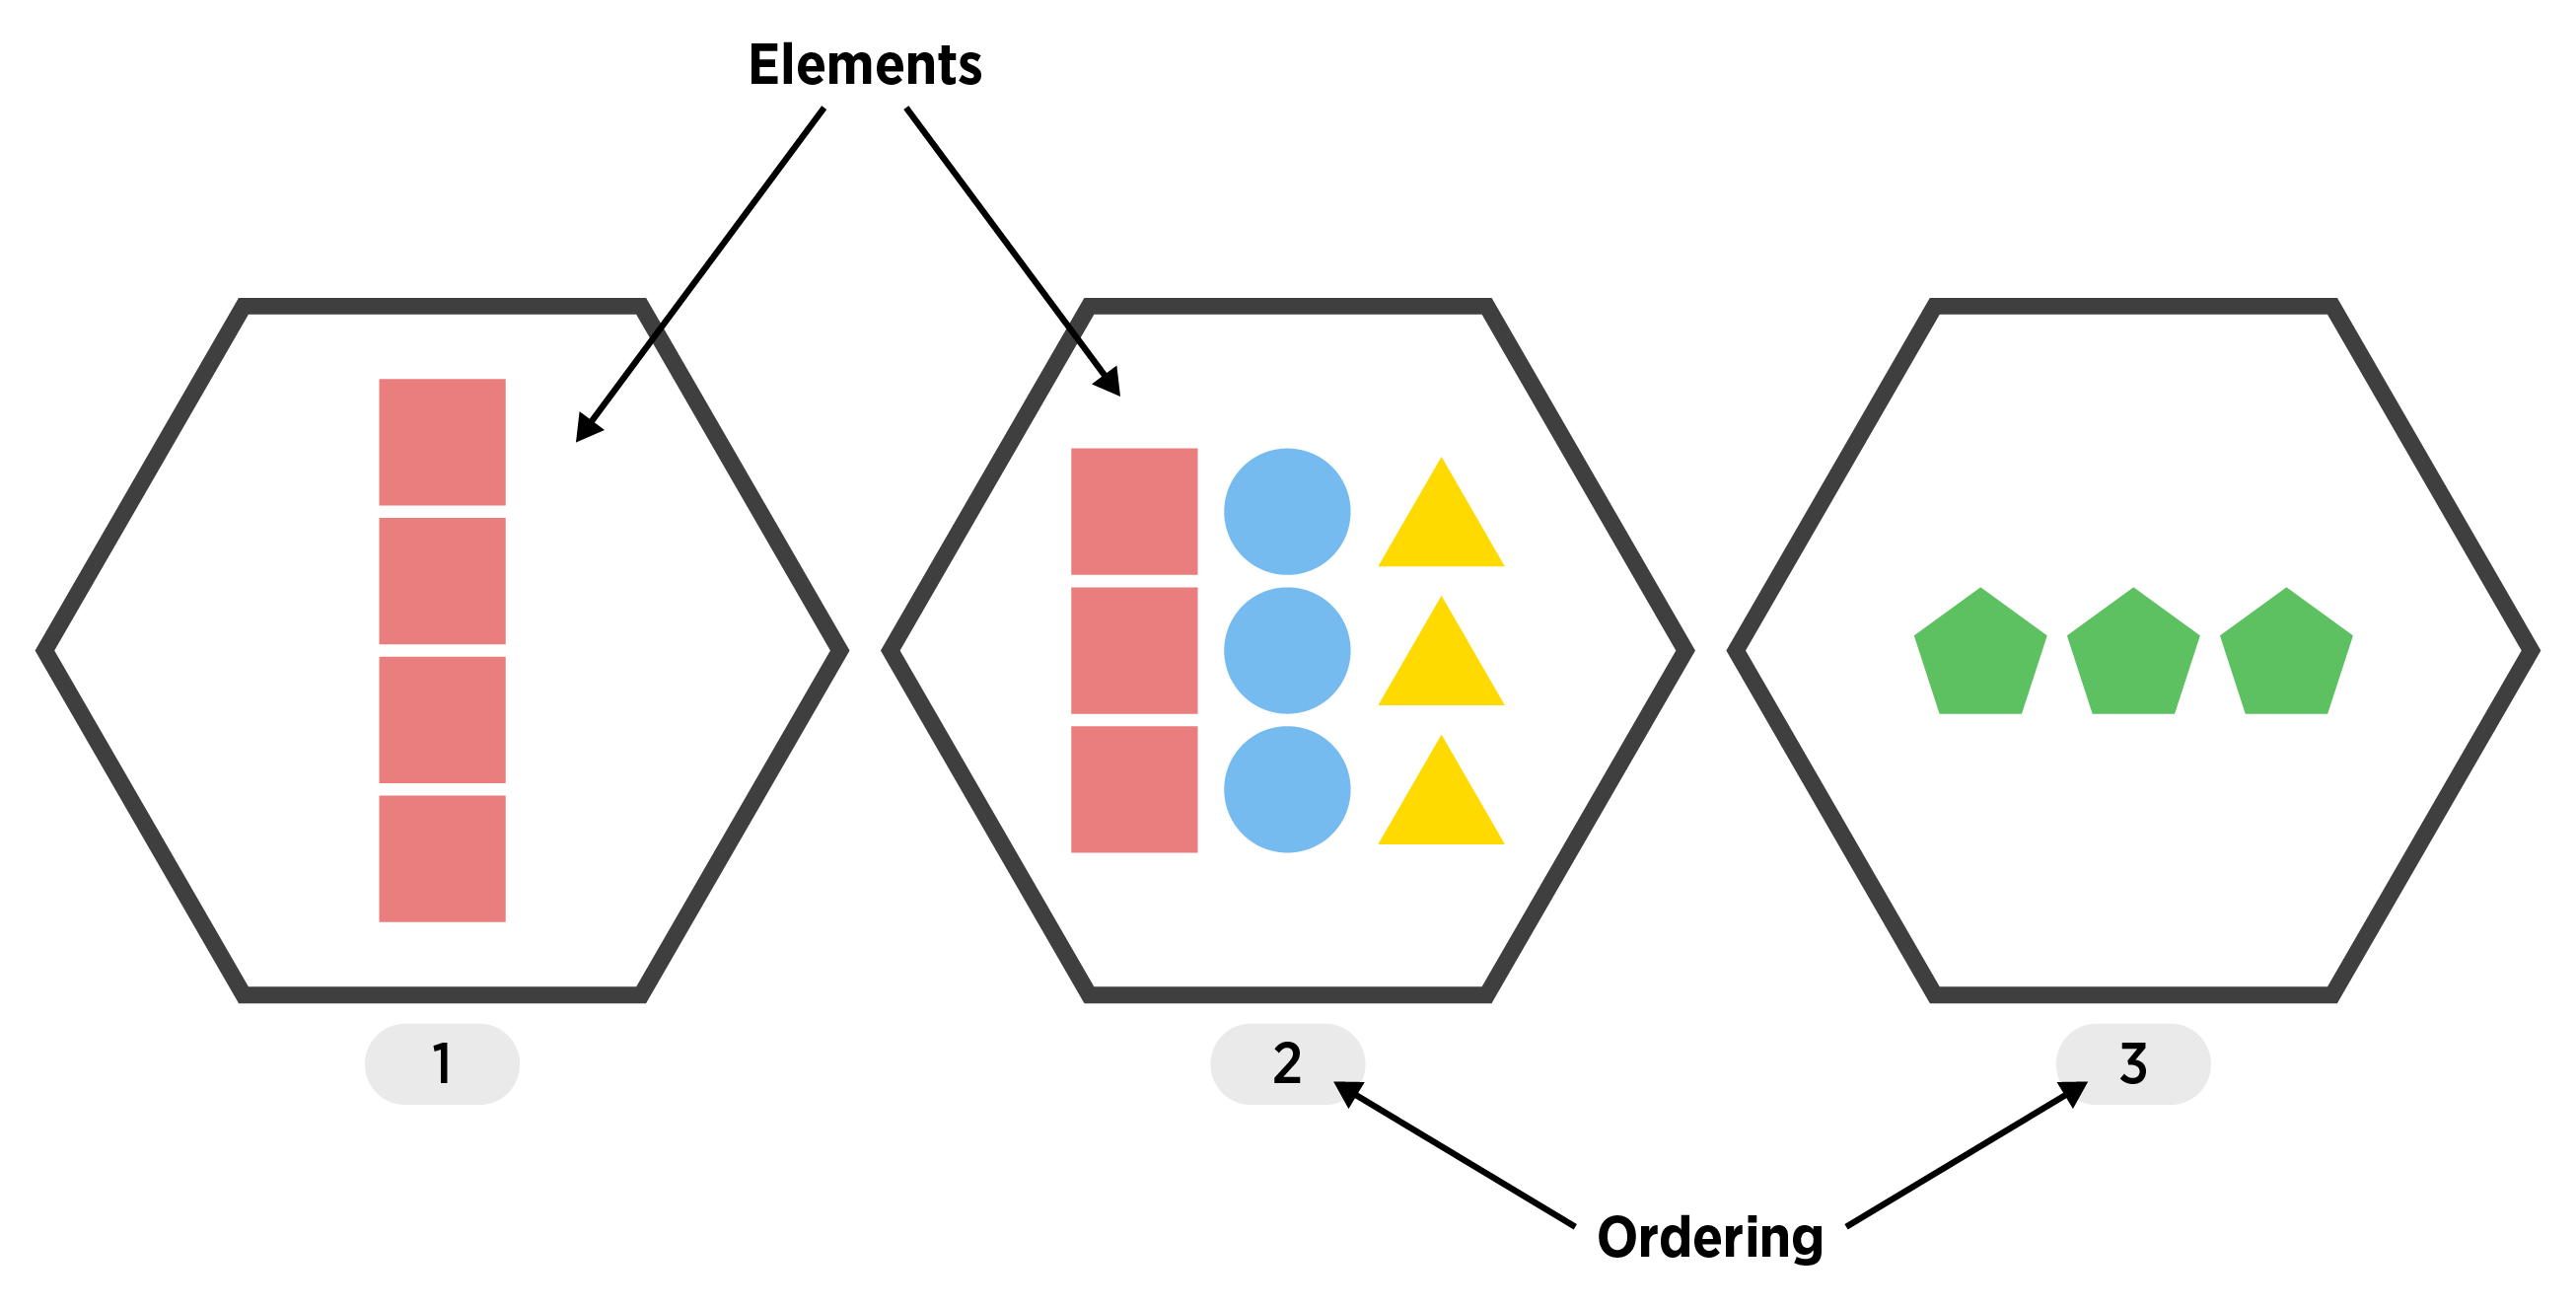
\includegraphics[width=0.8\linewidth]{img/listVisualF} \end{center}

A list can be created with the \texttt{list} function. You specify the elements you want to include, separated by commas.

\begin{Shaded}
\begin{Highlighting}[]
\KeywordTok{list}\NormalTok{(}\DecValTok{1}\OperatorTok{:}\DecValTok{3}\NormalTok{, }\KeywordTok{rnorm}\NormalTok{(}\DecValTok{2}\NormalTok{), }\KeywordTok{c}\NormalTok{(}\StringTok{"!"}\NormalTok{, }\StringTok{"?"}\NormalTok{))}
\end{Highlighting}
\end{Shaded}

\begin{verbatim}
## [[1]]
## [1] 1 2 3
## 
## [[2]]
## [1] 0.03012394 0.08541773
## 
## [[3]]
## [1] "!" "?"
\end{verbatim}

Similar to a data frame, you can add names to the list elements during creation.

\begin{Shaded}
\begin{Highlighting}[]
\KeywordTok{list}\NormalTok{(}\DataTypeTok{seq =} \DecValTok{1}\OperatorTok{:}\DecValTok{3}\NormalTok{, }\DataTypeTok{normVals =} \KeywordTok{rnorm}\NormalTok{(}\DecValTok{2}\NormalTok{), }\DataTypeTok{punctuation =} \KeywordTok{c}\NormalTok{(}\StringTok{"!"}\NormalTok{, }\StringTok{"?"}\NormalTok{))}
\end{Highlighting}
\end{Shaded}

\begin{verbatim}
## $seq
## [1] 1 2 3
## 
## $normVals
## [1]  1.116610 -1.218857
## 
## $punctuation
## [1] "!" "?"
\end{verbatim}

To recap, a list is a very flexible 1D object. It is really useful for more complex types of data.

The table below gives a summary of the data objects we've covered. For most data analysis you'll use data frames.

\begin{longtable}[]{@{}lll@{}}
\toprule
Dimension & Homogeneous & Heterogeneous\tabularnewline
\midrule
\endhead
1d & Atomic Vector & List\tabularnewline
2d & Matrix & Data Frame\tabularnewline
\bottomrule
\end{longtable}

Next we look at how to access or change parts of our these common data objects.

\hypertarget{accessing-common-data-objects-1}{%
\subsection{Accessing Common Data Objects}\label{accessing-common-data-objects-1}}

When we are dealing with a data object (1D or 2D) we may want to extract a single element, certain columns, or certain rows. In this section we'll look at how to subset or extract information from each of the common data objects covered in the previous section.

\hypertarget{atomic-vector-1d-1}{%
\subsubsection{Atomic Vector (1D)}\label{atomic-vector-1d-1}}

For atomic vectors (and lists, see later) you can return elements using square brackets \texttt{{[}{]}}. You may notice that when R prints a vector to the console you often see \texttt{{[}1{]}} next to the first element and perhaps a \texttt{{[}\#{]}} where R has to break and move to the next line of the console. The \texttt{{[}1{]}} implies the element printed next is the first element of the vector (R starts its counting at 1 not 0 like some other languages). The \texttt{{[}\#{]}} implies that the element printed to the right is the \texttt{\#} element of the vector. This is a good reminder of how to extract values from an atomic vector.

As an example, here we extract from a built-in R object called letters that is a vector of length 26 containing the letters of the alphabet.

\begin{Shaded}
\begin{Highlighting}[]
\NormalTok{letters }\CommentTok{#built-in vector}
\end{Highlighting}
\end{Shaded}

\begin{verbatim}
##  [1] "a" "b" "c" "d" "e" "f" "g" "h" "i" "j" "k" "l" "m" "n" "o" "p" "q" "r" "s"
## [20] "t" "u" "v" "w" "x" "y" "z"
\end{verbatim}

\begin{Shaded}
\begin{Highlighting}[]
\NormalTok{letters[}\DecValTok{1}\NormalTok{] }\CommentTok{#R starts counting at 1!}
\end{Highlighting}
\end{Shaded}

\begin{verbatim}
## [1] "a"
\end{verbatim}

\begin{Shaded}
\begin{Highlighting}[]
\NormalTok{letters[}\DecValTok{26}\NormalTok{]}
\end{Highlighting}
\end{Shaded}

\begin{verbatim}
## [1] "z"
\end{verbatim}

To obtain more than one element you can `feed' in a vector of indices to that you'd like to return.

\begin{Shaded}
\begin{Highlighting}[]
\NormalTok{letters[}\DecValTok{1}\OperatorTok{:}\DecValTok{4}\NormalTok{]}
\end{Highlighting}
\end{Shaded}

\begin{verbatim}
## [1] "a" "b" "c" "d"
\end{verbatim}

\begin{Shaded}
\begin{Highlighting}[]
\NormalTok{letters[}\KeywordTok{c}\NormalTok{(}\DecValTok{5}\NormalTok{, }\DecValTok{10}\NormalTok{, }\DecValTok{15}\NormalTok{, }\DecValTok{20}\NormalTok{, }\DecValTok{25}\NormalTok{)]}
\end{Highlighting}
\end{Shaded}

\begin{verbatim}
## [1] "e" "j" "o" "t" "y"
\end{verbatim}

\begin{Shaded}
\begin{Highlighting}[]
\NormalTok{x <-}\StringTok{ }\KeywordTok{c}\NormalTok{(}\DecValTok{1}\NormalTok{, }\DecValTok{2}\NormalTok{, }\DecValTok{5}\NormalTok{)}
\NormalTok{letters[x]}
\end{Highlighting}
\end{Shaded}

\begin{verbatim}
## [1] "a" "b" "e"
\end{verbatim}

If you'd like to return all values except a certain subset, you can use negative indices.

\begin{Shaded}
\begin{Highlighting}[]
\NormalTok{letters[}\OperatorTok{-}\NormalTok{(}\DecValTok{1}\OperatorTok{:}\DecValTok{4}\NormalTok{)]}
\end{Highlighting}
\end{Shaded}

\begin{verbatim}
##  [1] "e" "f" "g" "h" "i" "j" "k" "l" "m" "n" "o" "p" "q" "r" "s" "t" "u" "v" "w"
## [20] "x" "y" "z"
\end{verbatim}

\begin{Shaded}
\begin{Highlighting}[]
\NormalTok{x <-}\StringTok{ }\KeywordTok{c}\NormalTok{(}\DecValTok{1}\NormalTok{, }\DecValTok{2}\NormalTok{, }\DecValTok{5}\NormalTok{)}
\NormalTok{letters[}\OperatorTok{-}\NormalTok{x]}
\end{Highlighting}
\end{Shaded}

\begin{verbatim}
##  [1] "c" "d" "f" "g" "h" "i" "j" "k" "l" "m" "n" "o" "p" "q" "r" "s" "t" "u" "v"
## [20] "w" "x" "y" "z"
\end{verbatim}

\hypertarget{matrices-2d-1}{%
\subsubsection{Matrices (2D)}\label{matrices-2d-1}}

For rectangular data like a matrix you can return rectangular subsets using square brackets with a comma \texttt{{[}\ ,\ {]}}. Notice default row and column names when R prints a matrix!

\begin{Shaded}
\begin{Highlighting}[]
\NormalTok{mat <-}\StringTok{ }\KeywordTok{matrix}\NormalTok{(}\KeywordTok{c}\NormalTok{(}\DecValTok{1}\OperatorTok{:}\DecValTok{4}\NormalTok{, }\DecValTok{20}\OperatorTok{:}\DecValTok{17}\NormalTok{), }\DataTypeTok{ncol =} \DecValTok{2}\NormalTok{)}
\NormalTok{mat}
\end{Highlighting}
\end{Shaded}

\begin{verbatim}
##      [,1] [,2]
## [1,]    1   20
## [2,]    2   19
## [3,]    3   18
## [4,]    4   17
\end{verbatim}

This is a nice reminder of how to index a matrix. The value prior to the columns represents which row(s) you want to return and the value after the comma which column(s). If an index is left blank then all of that corresponding dimension (row or column) is returned.

\begin{Shaded}
\begin{Highlighting}[]
\NormalTok{mat[}\KeywordTok{c}\NormalTok{(}\DecValTok{2}\NormalTok{, }\DecValTok{4}\NormalTok{), ]}
\end{Highlighting}
\end{Shaded}

\begin{verbatim}
##      [,1] [,2]
## [1,]    2   19
## [2,]    4   17
\end{verbatim}

\begin{Shaded}
\begin{Highlighting}[]
\NormalTok{mat[, }\DecValTok{1}\NormalTok{]}
\end{Highlighting}
\end{Shaded}

\begin{verbatim}
## [1] 1 2 3 4
\end{verbatim}

\begin{Shaded}
\begin{Highlighting}[]
\NormalTok{mat[}\DecValTok{2}\NormalTok{, ]}
\end{Highlighting}
\end{Shaded}

\begin{verbatim}
## [1]  2 19
\end{verbatim}

\begin{Shaded}
\begin{Highlighting}[]
\NormalTok{mat[}\DecValTok{2}\NormalTok{, }\DecValTok{1}\NormalTok{]}
\end{Highlighting}
\end{Shaded}

\begin{verbatim}
## [1] 2
\end{verbatim}

Notice that R simplifies the result where possible. That is, returns an atomic vector if you have only 1 dimension and a matrix if two. This can be changed by adding an additional argument to the \texttt{{[}} function.

\begin{Shaded}
\begin{Highlighting}[]
\NormalTok{mat[ , }\DecValTok{1}\NormalTok{, drop =}\StringTok{ }\OtherTok{FALSE}\NormalTok{]}
\end{Highlighting}
\end{Shaded}

\begin{verbatim}
##      [,1]
## [1,]    1
## [2,]    2
## [3,]    3
## [4,]    4
\end{verbatim}

Also, if you only give a single value in the \texttt{{[}{]}} then R uses the count of the value in the matrix. Counts go down columns first.

\begin{Shaded}
\begin{Highlighting}[]
\NormalTok{mat[}\DecValTok{5}\NormalTok{]}
\end{Highlighting}
\end{Shaded}

\begin{verbatim}
## [1] 20
\end{verbatim}

If your matrix has column names associated with it, you can also use those to return columns of interest. To add column names we can look run \texttt{help(matrix)} to learn how! Notice the \texttt{dimnames} argument. You can specify names for the rows and columns by using a list with two vectors. The first vector indicating row names and the second column names. If we don't want to give rownames we can give a NULL (a special value in R that is used for undefined values - here giving no specification of row names). We can do this and give a character vector for the column names.

\begin{Shaded}
\begin{Highlighting}[]
\NormalTok{mat<-}\KeywordTok{matrix}\NormalTok{(}\KeywordTok{c}\NormalTok{(}\DecValTok{1}\OperatorTok{:}\DecValTok{4}\NormalTok{, }\DecValTok{20}\OperatorTok{:}\DecValTok{17}\NormalTok{), }\DataTypeTok{ncol =} \DecValTok{2}\NormalTok{,}
            \DataTypeTok{dimnames =} \KeywordTok{list}\NormalTok{(}\OtherTok{NULL}\NormalTok{, }\KeywordTok{c}\NormalTok{(}\StringTok{"First"}\NormalTok{, }\StringTok{"Second"}\NormalTok{))}
\NormalTok{            )}
\NormalTok{mat}
\end{Highlighting}
\end{Shaded}

\begin{verbatim}
##      First Second
## [1,]     1     20
## [2,]     2     19
## [3,]     3     18
## [4,]     4     17
\end{verbatim}

Now we can request columns be using a single name or a character vector of names.

\begin{Shaded}
\begin{Highlighting}[]
\NormalTok{mat[, }\StringTok{"First"}\NormalTok{]}
\end{Highlighting}
\end{Shaded}

\begin{verbatim}
## [1] 1 2 3 4
\end{verbatim}

To return all but certain parts of a matrix you can still use negative indices but note that this won't work with column names.

\begin{Shaded}
\begin{Highlighting}[]
\NormalTok{mat[}\OperatorTok{-}\KeywordTok{c}\NormalTok{(}\DecValTok{1}\NormalTok{,}\DecValTok{3}\NormalTok{), }\OperatorTok{-}\StringTok{"First"}\NormalTok{]}
\end{Highlighting}
\end{Shaded}

\begin{verbatim}
## Error in -"First": invalid argument to unary operator
\end{verbatim}

\begin{Shaded}
\begin{Highlighting}[]
\NormalTok{mat[}\OperatorTok{-}\KeywordTok{c}\NormalTok{(}\DecValTok{1}\NormalTok{,}\DecValTok{3}\NormalTok{), }\StringTok{"First"}\NormalTok{]}
\end{Highlighting}
\end{Shaded}

\begin{verbatim}
## [1] 2 4
\end{verbatim}

\hypertarget{data-frames-2d-1}{%
\subsubsection{Data Frames (2D)}\label{data-frames-2d-1}}

Since a data frame is also a rectangular data object you can return rectangular subsets using square brackets with a comma \texttt{{[}\ ,\ {]}}!

As an example, we'll subset the built-in \texttt{iris} data frame. To get an idea about this object we can run \texttt{str(iris)}.

\begin{Shaded}
\begin{Highlighting}[]
\KeywordTok{str}\NormalTok{(iris)}
\end{Highlighting}
\end{Shaded}

\begin{verbatim}
## 'data.frame':    150 obs. of  6 variables:
##  $ Sepal.Length: num  5.1 4.9 4.7 4.6 5 5.4 4.6 5 4.4 4.9 ...
##  $ Sepal.Width : num  3.5 3 3.2 3.1 3.6 3.9 3.4 3.4 2.9 3.1 ...
##  $ Petal.Length: num  1.4 1.4 1.3 1.5 1.4 1.7 1.4 1.5 1.4 1.5 ...
##  $ Petal.Width : num  0.2 0.2 0.2 0.2 0.2 0.4 0.3 0.2 0.2 0.1 ...
##  $ Species     : Factor w/ 3 levels "setosa","versicolor",..: 1 1 1 1 1 1 1 1 1 1 ...
##  $ extra       : chr  "a" "a" "a" "a" ...
\end{verbatim}

We can see this is a data frame with a few columns, four are numeric and one is a factor (a special type of character vector essentially - these will be covered when we discuss plotting).

\begin{Shaded}
\begin{Highlighting}[]
\NormalTok{iris[}\DecValTok{1}\OperatorTok{:}\DecValTok{4}\NormalTok{, }\DecValTok{2}\OperatorTok{:}\DecValTok{4}\NormalTok{]}
\end{Highlighting}
\end{Shaded}

\begin{verbatim}
##   Sepal.Width Petal.Length Petal.Width
## 1         3.5          1.4         0.2
## 2         3.0          1.4         0.2
## 3         3.2          1.3         0.2
## 4         3.1          1.5         0.2
\end{verbatim}

\begin{Shaded}
\begin{Highlighting}[]
\NormalTok{iris[}\DecValTok{1}\NormalTok{, ]}
\end{Highlighting}
\end{Shaded}

\begin{verbatim}
##   Sepal.Length Sepal.Width Petal.Length Petal.Width Species extra
## 1          5.1         3.5          1.4         0.2  setosa     a
\end{verbatim}

\begin{Shaded}
\begin{Highlighting}[]
\NormalTok{iris[, }\DecValTok{1}\NormalTok{]}
\end{Highlighting}
\end{Shaded}

\begin{verbatim}
##   [1] 5.1 4.9 4.7 4.6 5.0 5.4 4.6 5.0 4.4 4.9 5.4 4.8 4.8 4.3 5.8 5.7 5.4 5.1
##  [19] 5.7 5.1 5.4 5.1 4.6 5.1 4.8 5.0 5.0 5.2 5.2 4.7 4.8 5.4 5.2 5.5 4.9 5.0
##  [37] 5.5 4.9 4.4 5.1 5.0 4.5 4.4 5.0 5.1 4.8 5.1 4.6 5.3 5.0 7.0 6.4 6.9 5.5
##  [55] 6.5 5.7 6.3 4.9 6.6 5.2 5.0 5.9 6.0 6.1 5.6 6.7 5.6 5.8 6.2 5.6 5.9 6.1
##  [73] 6.3 6.1 6.4 6.6 6.8 6.7 6.0 5.7 5.5 5.5 5.8 6.0 5.4 6.0 6.7 6.3 5.6 5.5
##  [91] 5.5 6.1 5.8 5.0 5.6 5.7 5.7 6.2 5.1 5.7
##  [ reached getOption("max.print") -- omitted 50 entries ]
\end{verbatim}

Notice the simplification done when a single column is selected. R will simplify to a vector unless \texttt{drop\ =\ FALSE} is included as done in the matrix section. (The simplification doesn't occur when a single row is selected because data frames are actually lists - we'll discuss this more in the list section!)

You can use columns names to subset as well.

\begin{Shaded}
\begin{Highlighting}[]
\NormalTok{iris[}\DecValTok{1}\OperatorTok{:}\DecValTok{10}\NormalTok{ , }\KeywordTok{c}\NormalTok{(}\StringTok{"Sepal.Length"}\NormalTok{, }\StringTok{"Species"}\NormalTok{)]}
\end{Highlighting}
\end{Shaded}

\begin{verbatim}
##    Sepal.Length Species
## 1           5.1  setosa
## 2           4.9  setosa
## 3           4.7  setosa
## 4           4.6  setosa
## 5           5.0  setosa
## 6           5.4  setosa
## 7           4.6  setosa
## 8           5.0  setosa
## 9           4.4  setosa
## 10          4.9  setosa
\end{verbatim}

The most common way to access a single columns is to use the dollar sign operator.

\begin{Shaded}
\begin{Highlighting}[]
\NormalTok{iris}\OperatorTok{$}\NormalTok{Sepal.Length}
\end{Highlighting}
\end{Shaded}

\begin{verbatim}
##   [1] 5.1 4.9 4.7 4.6 5.0 5.4 4.6 5.0 4.4 4.9 5.4 4.8 4.8 4.3 5.8 5.7 5.4 5.1
##  [19] 5.7 5.1 5.4 5.1 4.6 5.1 4.8 5.0 5.0 5.2 5.2 4.7 4.8 5.4 5.2 5.5 4.9 5.0
##  [37] 5.5 4.9 4.4 5.1 5.0 4.5 4.4 5.0 5.1 4.8 5.1 4.6 5.3 5.0 7.0 6.4 6.9 5.5
##  [55] 6.5 5.7 6.3 4.9 6.6 5.2 5.0 5.9 6.0 6.1 5.6 6.7 5.6 5.8 6.2 5.6 5.9 6.1
##  [73] 6.3 6.1 6.4 6.6 6.8 6.7 6.0 5.7 5.5 5.5 5.8 6.0 5.4 6.0 6.7 6.3 5.6 5.5
##  [91] 5.5 6.1 5.8 5.0 5.6 5.7 5.7 6.2 5.1 5.7
##  [ reached getOption("max.print") -- omitted 50 entries ]
\end{verbatim}

A nice benefit of using RStudio is that column names will be filled in automatically as you type. In your console do the following:

\begin{itemize}
\tightlist
\item
  Type \texttt{iris\$}\\
\item
  If no choices - hit tab
\item
  Scroll up and down or continue typing to highlight the column of interest\\
\item
  Hit tab again to choose
\end{itemize}

\hypertarget{lists-1d-1}{%
\subsubsection{Lists (1D)}\label{lists-1d-1}}

As a list is a 1D data object we can use single square brackets \texttt{{[}\ {]}} for multiple list elements.

\begin{Shaded}
\begin{Highlighting}[]
\NormalTok{x <-}\StringTok{ }\KeywordTok{list}\NormalTok{(}\StringTok{"HI"}\NormalTok{, }\KeywordTok{c}\NormalTok{(}\DecValTok{10}\OperatorTok{:}\DecValTok{20}\NormalTok{), }\DecValTok{1}\NormalTok{)}
\NormalTok{x}
\end{Highlighting}
\end{Shaded}

\begin{verbatim}
## [[1]]
## [1] "HI"
## 
## [[2]]
##  [1] 10 11 12 13 14 15 16 17 18 19 20
## 
## [[3]]
## [1] 1
\end{verbatim}

\begin{Shaded}
\begin{Highlighting}[]
\NormalTok{x[}\DecValTok{2}\OperatorTok{:}\DecValTok{3}\NormalTok{]}
\end{Highlighting}
\end{Shaded}

\begin{verbatim}
## [[1]]
##  [1] 10 11 12 13 14 15 16 17 18 19 20
## 
## [[2]]
## [1] 1
\end{verbatim}

We can use double square brackets \texttt{{[}{[}\ {]}{]}} (or \texttt{{[}\ {]}}) to return a single list element. The major difference is in whether or not a list with the element chosen is returned or just the element itself. \texttt{{[}{[}} will return just the element requested.

\begin{Shaded}
\begin{Highlighting}[]
\NormalTok{x <-}\StringTok{ }\KeywordTok{list}\NormalTok{(}\StringTok{"HI"}\NormalTok{, }\KeywordTok{c}\NormalTok{(}\DecValTok{10}\OperatorTok{:}\DecValTok{20}\NormalTok{), }\DecValTok{1}\NormalTok{)}
\NormalTok{x[}\DecValTok{1}\NormalTok{]}
\end{Highlighting}
\end{Shaded}

\begin{verbatim}
## [[1]]
## [1] "HI"
\end{verbatim}

\begin{Shaded}
\begin{Highlighting}[]
\NormalTok{x[[}\DecValTok{1}\NormalTok{]]}
\end{Highlighting}
\end{Shaded}

\begin{verbatim}
## [1] "HI"
\end{verbatim}

\begin{Shaded}
\begin{Highlighting}[]
\NormalTok{x[[}\DecValTok{2}\NormalTok{]]}
\end{Highlighting}
\end{Shaded}

\begin{verbatim}
##  [1] 10 11 12 13 14 15 16 17 18 19 20
\end{verbatim}

\begin{Shaded}
\begin{Highlighting}[]
\NormalTok{x[[}\DecValTok{2}\NormalTok{]][}\DecValTok{4}\OperatorTok{:}\DecValTok{5}\NormalTok{]}
\end{Highlighting}
\end{Shaded}

\begin{verbatim}
## [1] 13 14
\end{verbatim}

Recall we could name our list elements. If they are named we can use the \texttt{\$} similar to a data frame.

\begin{Shaded}
\begin{Highlighting}[]
\NormalTok{x <-}\StringTok{ }\KeywordTok{list}\NormalTok{(}\StringTok{"HI"}\NormalTok{, }\KeywordTok{c}\NormalTok{(}\DecValTok{10}\OperatorTok{:}\DecValTok{20}\NormalTok{), }\DecValTok{1}\NormalTok{)}
\KeywordTok{str}\NormalTok{(x)}
\end{Highlighting}
\end{Shaded}

\begin{verbatim}
## List of 3
##  $ : chr "HI"
##  $ : int [1:11] 10 11 12 13 14 15 16 17 18 19 ...
##  $ : num 1
\end{verbatim}

\begin{Shaded}
\begin{Highlighting}[]
\NormalTok{x <-}\StringTok{ }\KeywordTok{list}\NormalTok{(}\DataTypeTok{First =} \StringTok{"Hi"}\NormalTok{, }\DataTypeTok{Second =} \KeywordTok{c}\NormalTok{(}\DecValTok{10}\OperatorTok{:}\DecValTok{20}\NormalTok{), }\DataTypeTok{Third =} \DecValTok{1}\NormalTok{)}
\NormalTok{x}\OperatorTok{$}\NormalTok{Second}
\end{Highlighting}
\end{Shaded}

\begin{verbatim}
##  [1] 10 11 12 13 14 15 16 17 18 19 20
\end{verbatim}

Under the hood a data frame is just a \emph{list} of equal length vectors!

\begin{Shaded}
\begin{Highlighting}[]
\KeywordTok{str}\NormalTok{(x)}
\end{Highlighting}
\end{Shaded}

\begin{verbatim}
## List of 3
##  $ First : chr "Hi"
##  $ Second: int [1:11] 10 11 12 13 14 15 16 17 18 19 ...
##  $ Third : num 1
\end{verbatim}

\begin{Shaded}
\begin{Highlighting}[]
\KeywordTok{str}\NormalTok{(iris)}
\end{Highlighting}
\end{Shaded}

\begin{verbatim}
## 'data.frame':    150 obs. of  6 variables:
##  $ Sepal.Length: num  5.1 4.9 4.7 4.6 5 5.4 4.6 5 4.4 4.9 ...
##  $ Sepal.Width : num  3.5 3 3.2 3.1 3.6 3.9 3.4 3.4 2.9 3.1 ...
##  $ Petal.Length: num  1.4 1.4 1.3 1.5 1.4 1.7 1.4 1.5 1.4 1.5 ...
##  $ Petal.Width : num  0.2 0.2 0.2 0.2 0.2 0.4 0.3 0.2 0.2 0.1 ...
##  $ Species     : Factor w/ 3 levels "setosa","versicolor",..: 1 1 1 1 1 1 1 1 1 1 ...
##  $ extra       : chr  "a" "a" "a" "a" ...
\end{verbatim}

\begin{Shaded}
\begin{Highlighting}[]
\KeywordTok{typeof}\NormalTok{(x)}
\end{Highlighting}
\end{Shaded}

\begin{verbatim}
## [1] "list"
\end{verbatim}

\begin{Shaded}
\begin{Highlighting}[]
\KeywordTok{typeof}\NormalTok{(iris)}
\end{Highlighting}
\end{Shaded}

\begin{verbatim}
## [1] "list"
\end{verbatim}

This means we can index a data frame in a similar way to how we index a list if we want.

\begin{Shaded}
\begin{Highlighting}[]
\NormalTok{iris[[}\DecValTok{2}\NormalTok{]]}
\end{Highlighting}
\end{Shaded}

\begin{verbatim}
##   [1] 3.5 3.0 3.2 3.1 3.6 3.9 3.4 3.4 2.9 3.1 3.7 3.4 3.0 3.0 4.0 4.4 3.9 3.5
##  [19] 3.8 3.8 3.4 3.7 3.6 3.3 3.4 3.0 3.4 3.5 3.4 3.2 3.1 3.4 4.1 4.2 3.1 3.2
##  [37] 3.5 3.6 3.0 3.4 3.5 2.3 3.2 3.5 3.8 3.0 3.8 3.2 3.7 3.3 3.2 3.2 3.1 2.3
##  [55] 2.8 2.8 3.3 2.4 2.9 2.7 2.0 3.0 2.2 2.9 2.9 3.1 3.0 2.7 2.2 2.5 3.2 2.8
##  [73] 2.5 2.8 2.9 3.0 2.8 3.0 2.9 2.6 2.4 2.4 2.7 2.7 3.0 3.4 3.1 2.3 3.0 2.5
##  [91] 2.6 3.0 2.6 2.3 2.7 3.0 2.9 2.9 2.5 2.8
##  [ reached getOption("max.print") -- omitted 50 entries ]
\end{verbatim}

Lastly, one nice thing about lists (and data frames) is that you can use partial matching with \texttt{{[}{[}} and \texttt{\$}.

\begin{Shaded}
\begin{Highlighting}[]
\NormalTok{iris}\OperatorTok{$}\NormalTok{Sp[}\DecValTok{1}\OperatorTok{:}\DecValTok{10}\NormalTok{]}
\end{Highlighting}
\end{Shaded}

\begin{verbatim}
##  [1] setosa setosa setosa setosa setosa setosa setosa setosa setosa setosa
## Levels: setosa versicolor virginica
\end{verbatim}

\begin{Shaded}
\begin{Highlighting}[]
\NormalTok{iris[[}\StringTok{"Petal.Len"}\NormalTok{, exact =}\StringTok{ }\OtherTok{FALSE}\NormalTok{]]}
\end{Highlighting}
\end{Shaded}

\begin{verbatim}
##   [1] 1.4 1.4 1.3 1.5 1.4 1.7 1.4 1.5 1.4 1.5 1.5 1.6 1.4 1.1 1.2 1.5 1.3 1.4
##  [19] 1.7 1.5 1.7 1.5 1.0 1.7 1.9 1.6 1.6 1.5 1.4 1.6 1.6 1.5 1.5 1.4 1.5 1.2
##  [37] 1.3 1.4 1.3 1.5 1.3 1.3 1.3 1.6 1.9 1.4 1.6 1.4 1.5 1.4 4.7 4.5 4.9 4.0
##  [55] 4.6 4.5 4.7 3.3 4.6 3.9 3.5 4.2 4.0 4.7 3.6 4.4 4.5 4.1 4.5 3.9 4.8 4.0
##  [73] 4.9 4.7 4.3 4.4 4.8 5.0 4.5 3.5 3.8 3.7 3.9 5.1 4.5 4.5 4.7 4.4 4.1 4.0
##  [91] 4.4 4.6 4.0 3.3 4.2 4.2 4.2 4.3 3.0 4.1
##  [ reached getOption("max.print") -- omitted 50 entries ]
\end{verbatim}

This is less important now that RStudio can auto-complete long column names.

\hypertarget{basics-of-r-recap-1}{%
\subsection{Basics of R Recap}\label{basics-of-r-recap-1}}

\begin{itemize}
\item
  RStudio IDE (Integrated Development Environment)
\item
  R Objects and Classes
\item
  Data Objects \& Basic Manipulation
\end{itemize}

\begin{longtable}[]{@{}lll@{}}
\toprule
Dimension & Homogeneous & Heterogeneous\tabularnewline
\midrule
\endhead
1d & Atomic Vector & List\tabularnewline
2d & Matrix & Data Frame\tabularnewline
\bottomrule
\end{longtable}

Basic access via

\begin{itemize}
\item
  Atomic vectors - \texttt{x{[}\ {]}}
\item
  Matrices - \texttt{x{[}\ ,\ {]}}
\item
  Data Frames - \texttt{x{[}\ ,\ {]}} or \texttt{x\$name}
\item
  Lists - \texttt{x{[}\ {]}}, \texttt{x{[}{[}\ {]}{]}}, or \texttt{x\$name}
\end{itemize}

\hypertarget{data-manipulation-ideas-1}{%
\subsection{Data Manipulation Ideas}\label{data-manipulation-ideas-1}}

As you can see it isn't too difficult to bring well structured raw data into R. You should now have the basics of reading in delimited, Excel, SAS, SPSS, JSON, and XML data as well as how to connect to a database and contact an API. Once you have your data you may want to manipulate it in some way.

Often we want to grab only certain types of observations (filter rows).

\begin{center}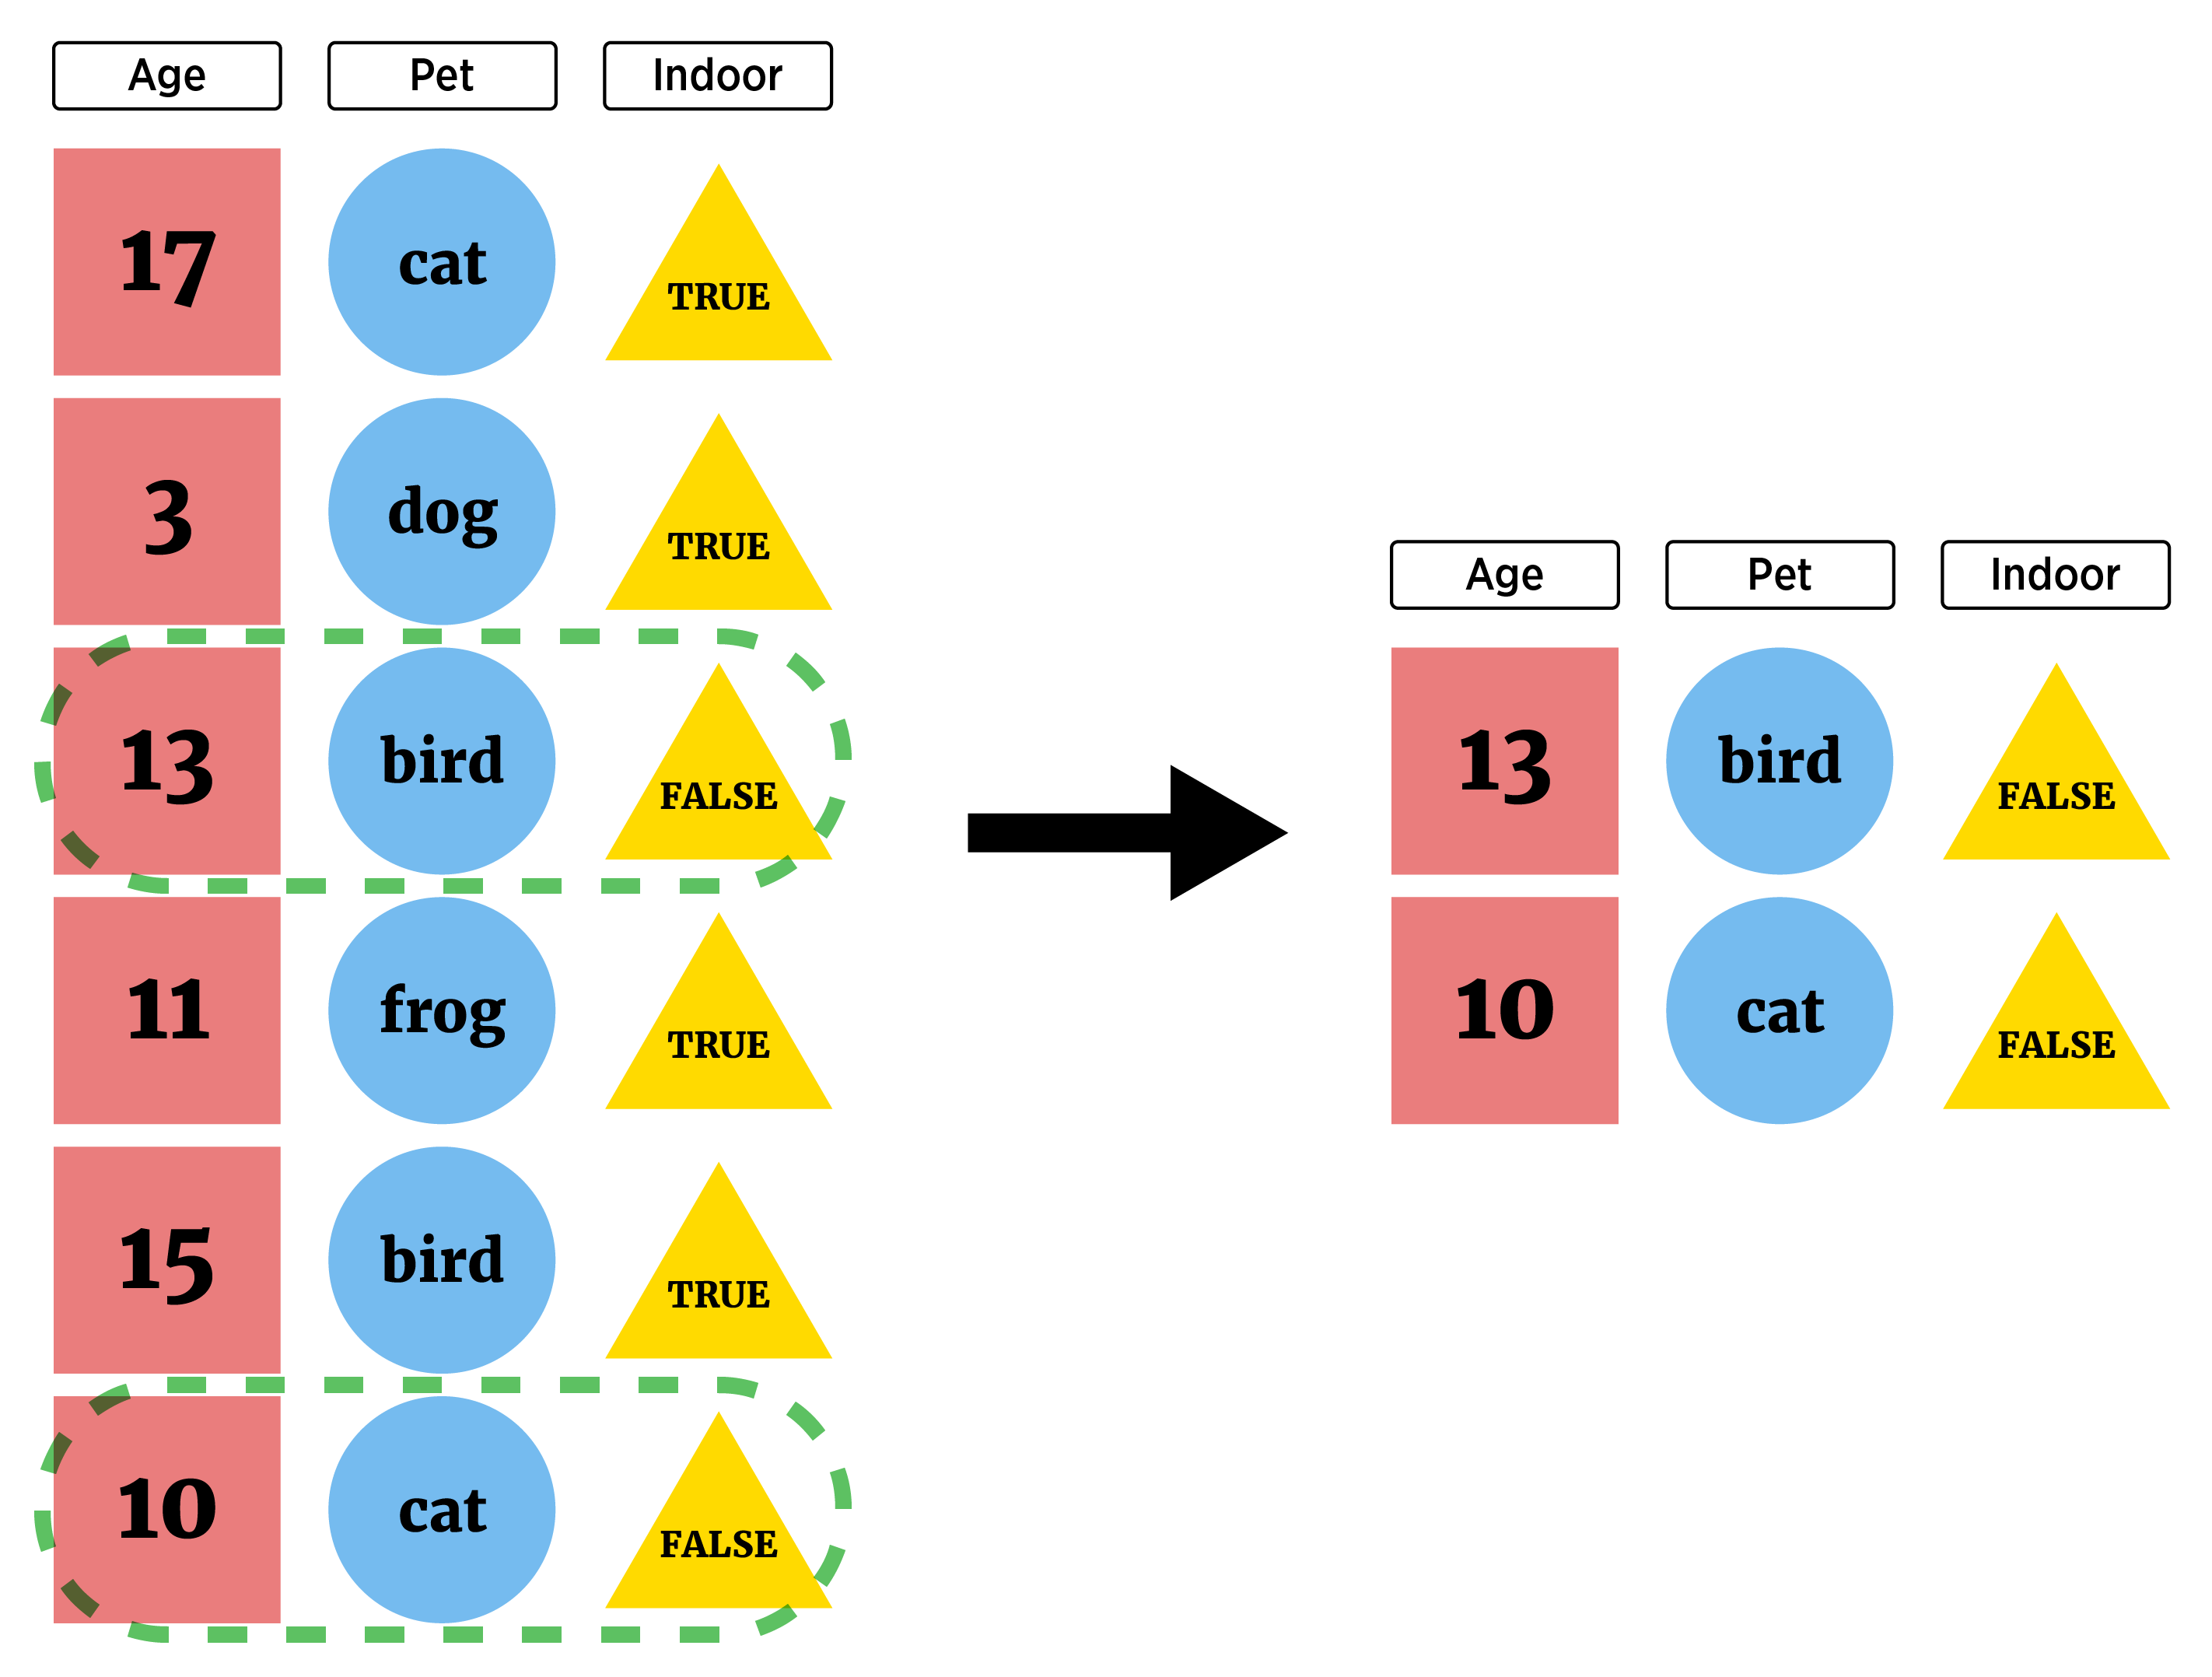
\includegraphics[width=0.8\linewidth]{img/filterVisualF} \end{center}

We also want to only look at only certain variables (select columns).

\begin{center}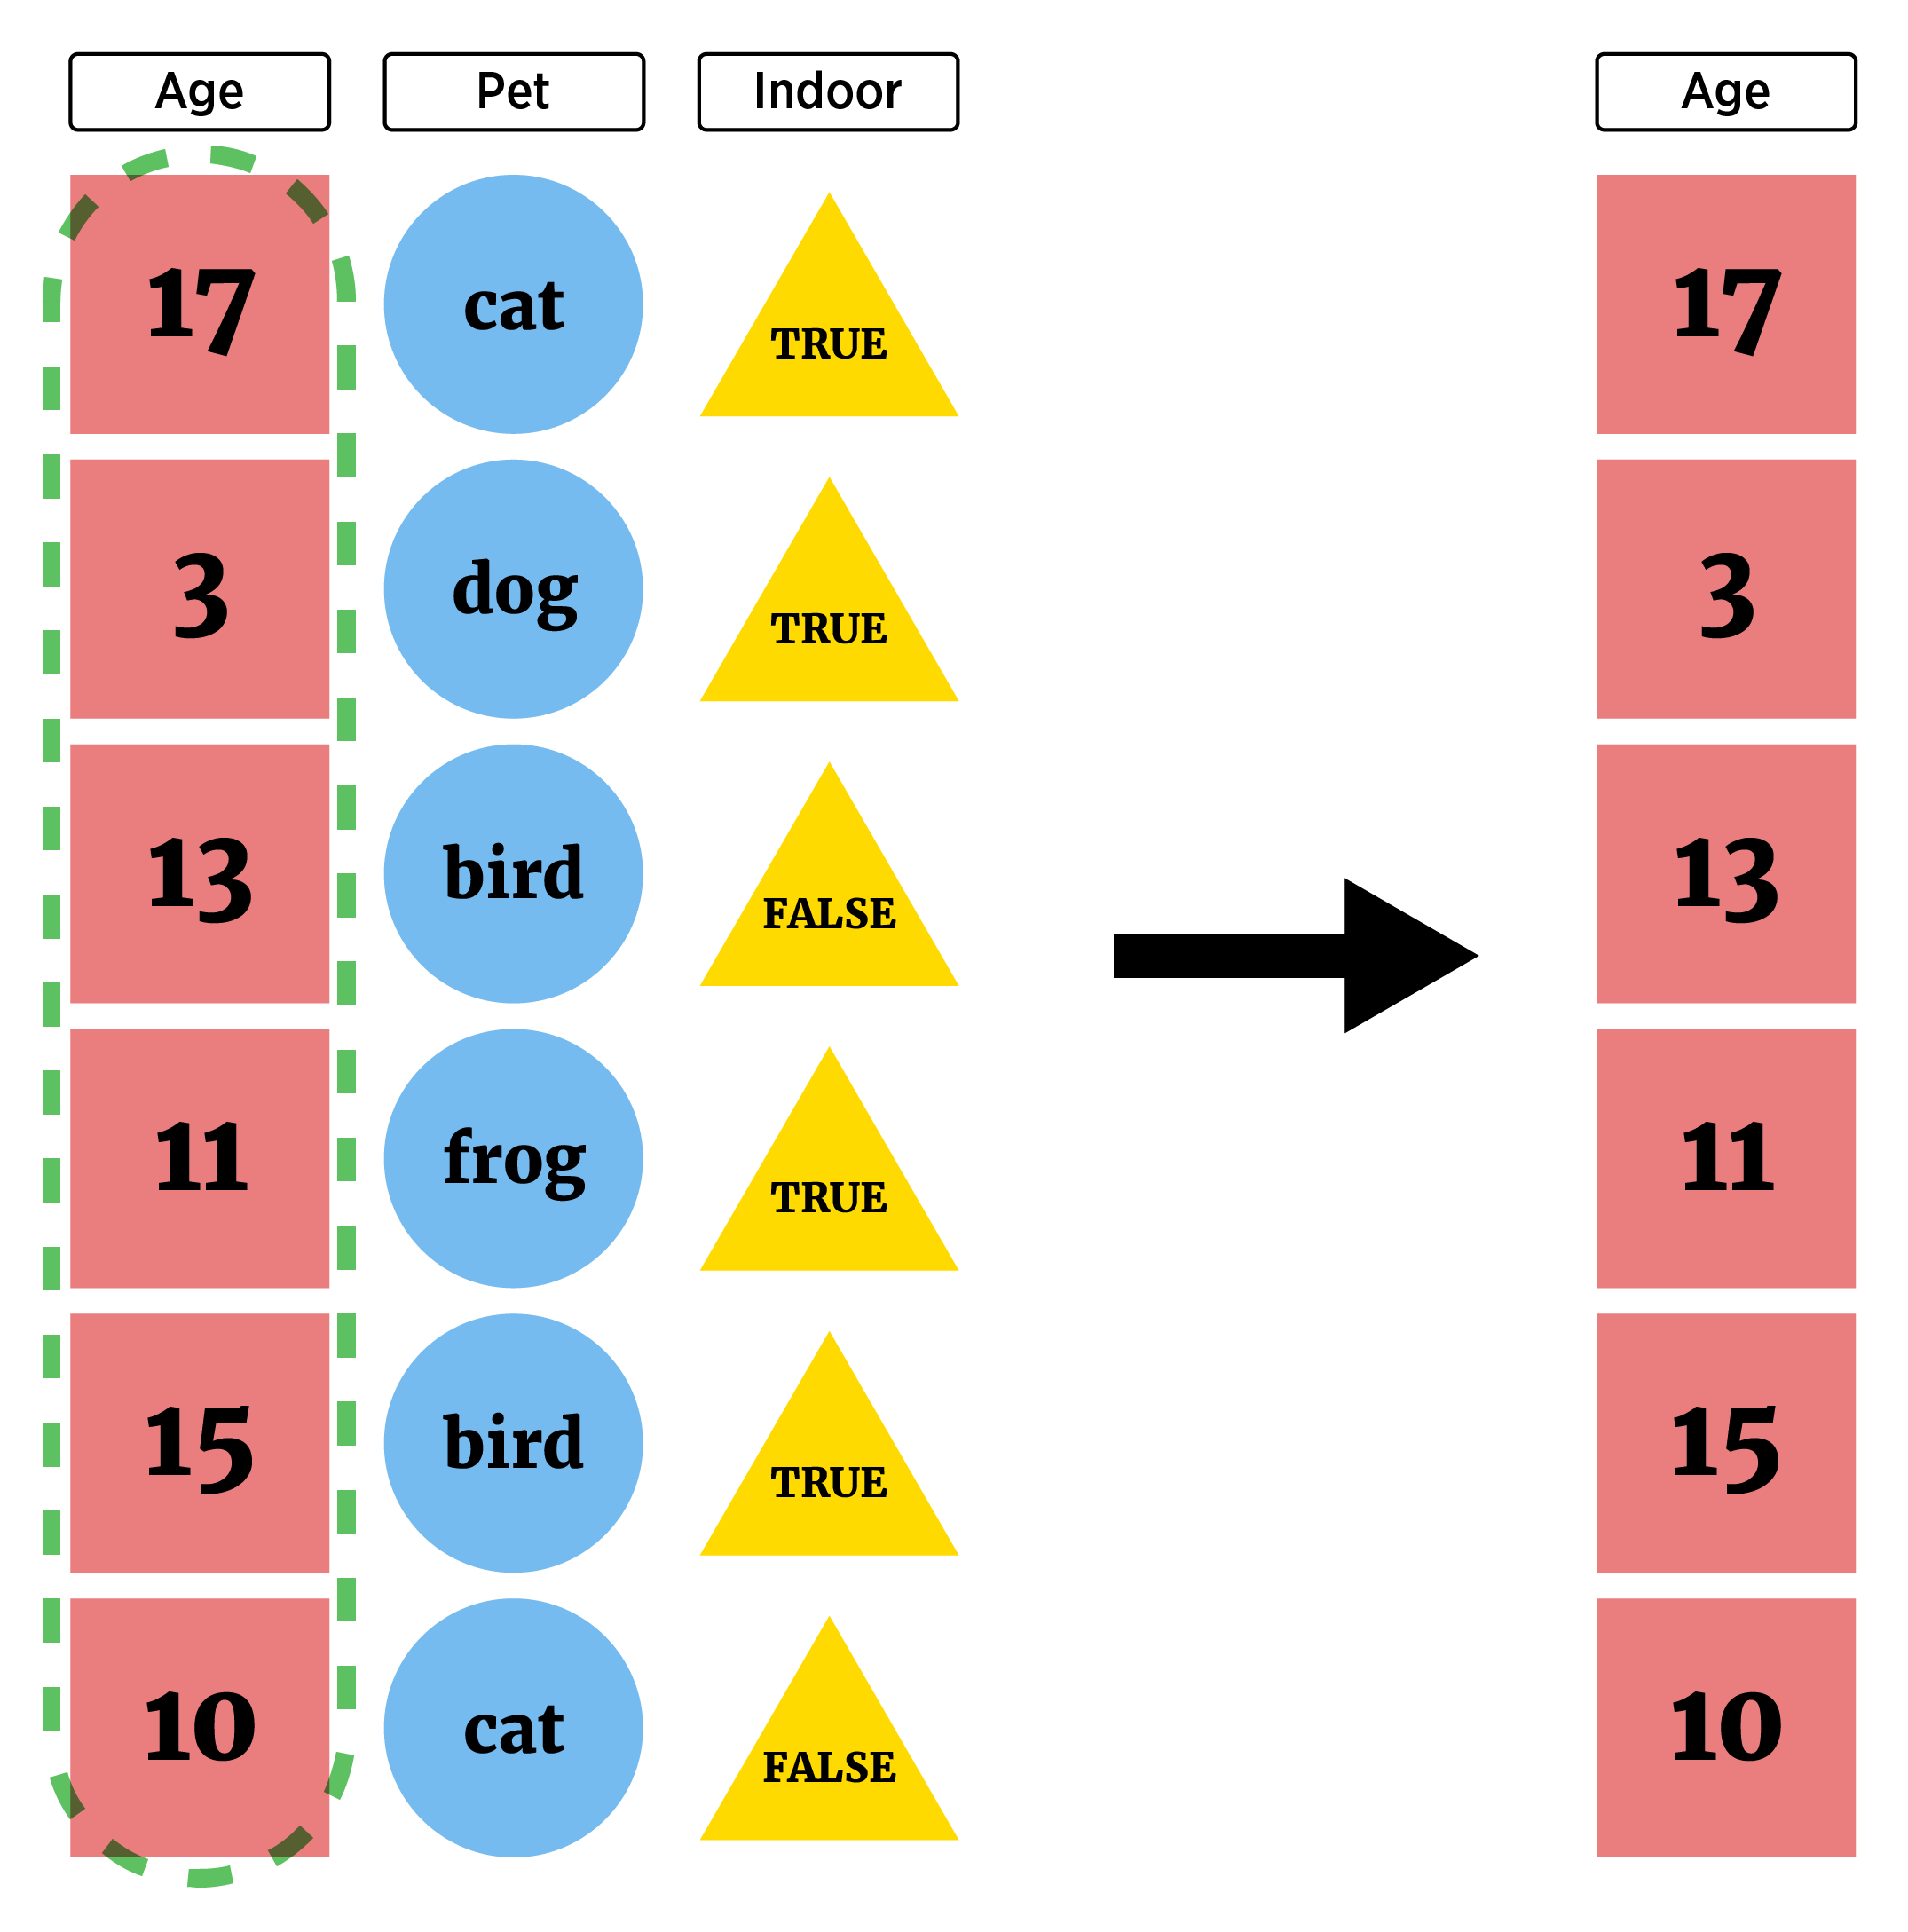
\includegraphics[width=0.7\linewidth]{img/selectVisualF} \end{center}

Other times we want to create new variables that may be functions of the data in the data set.

\begin{center}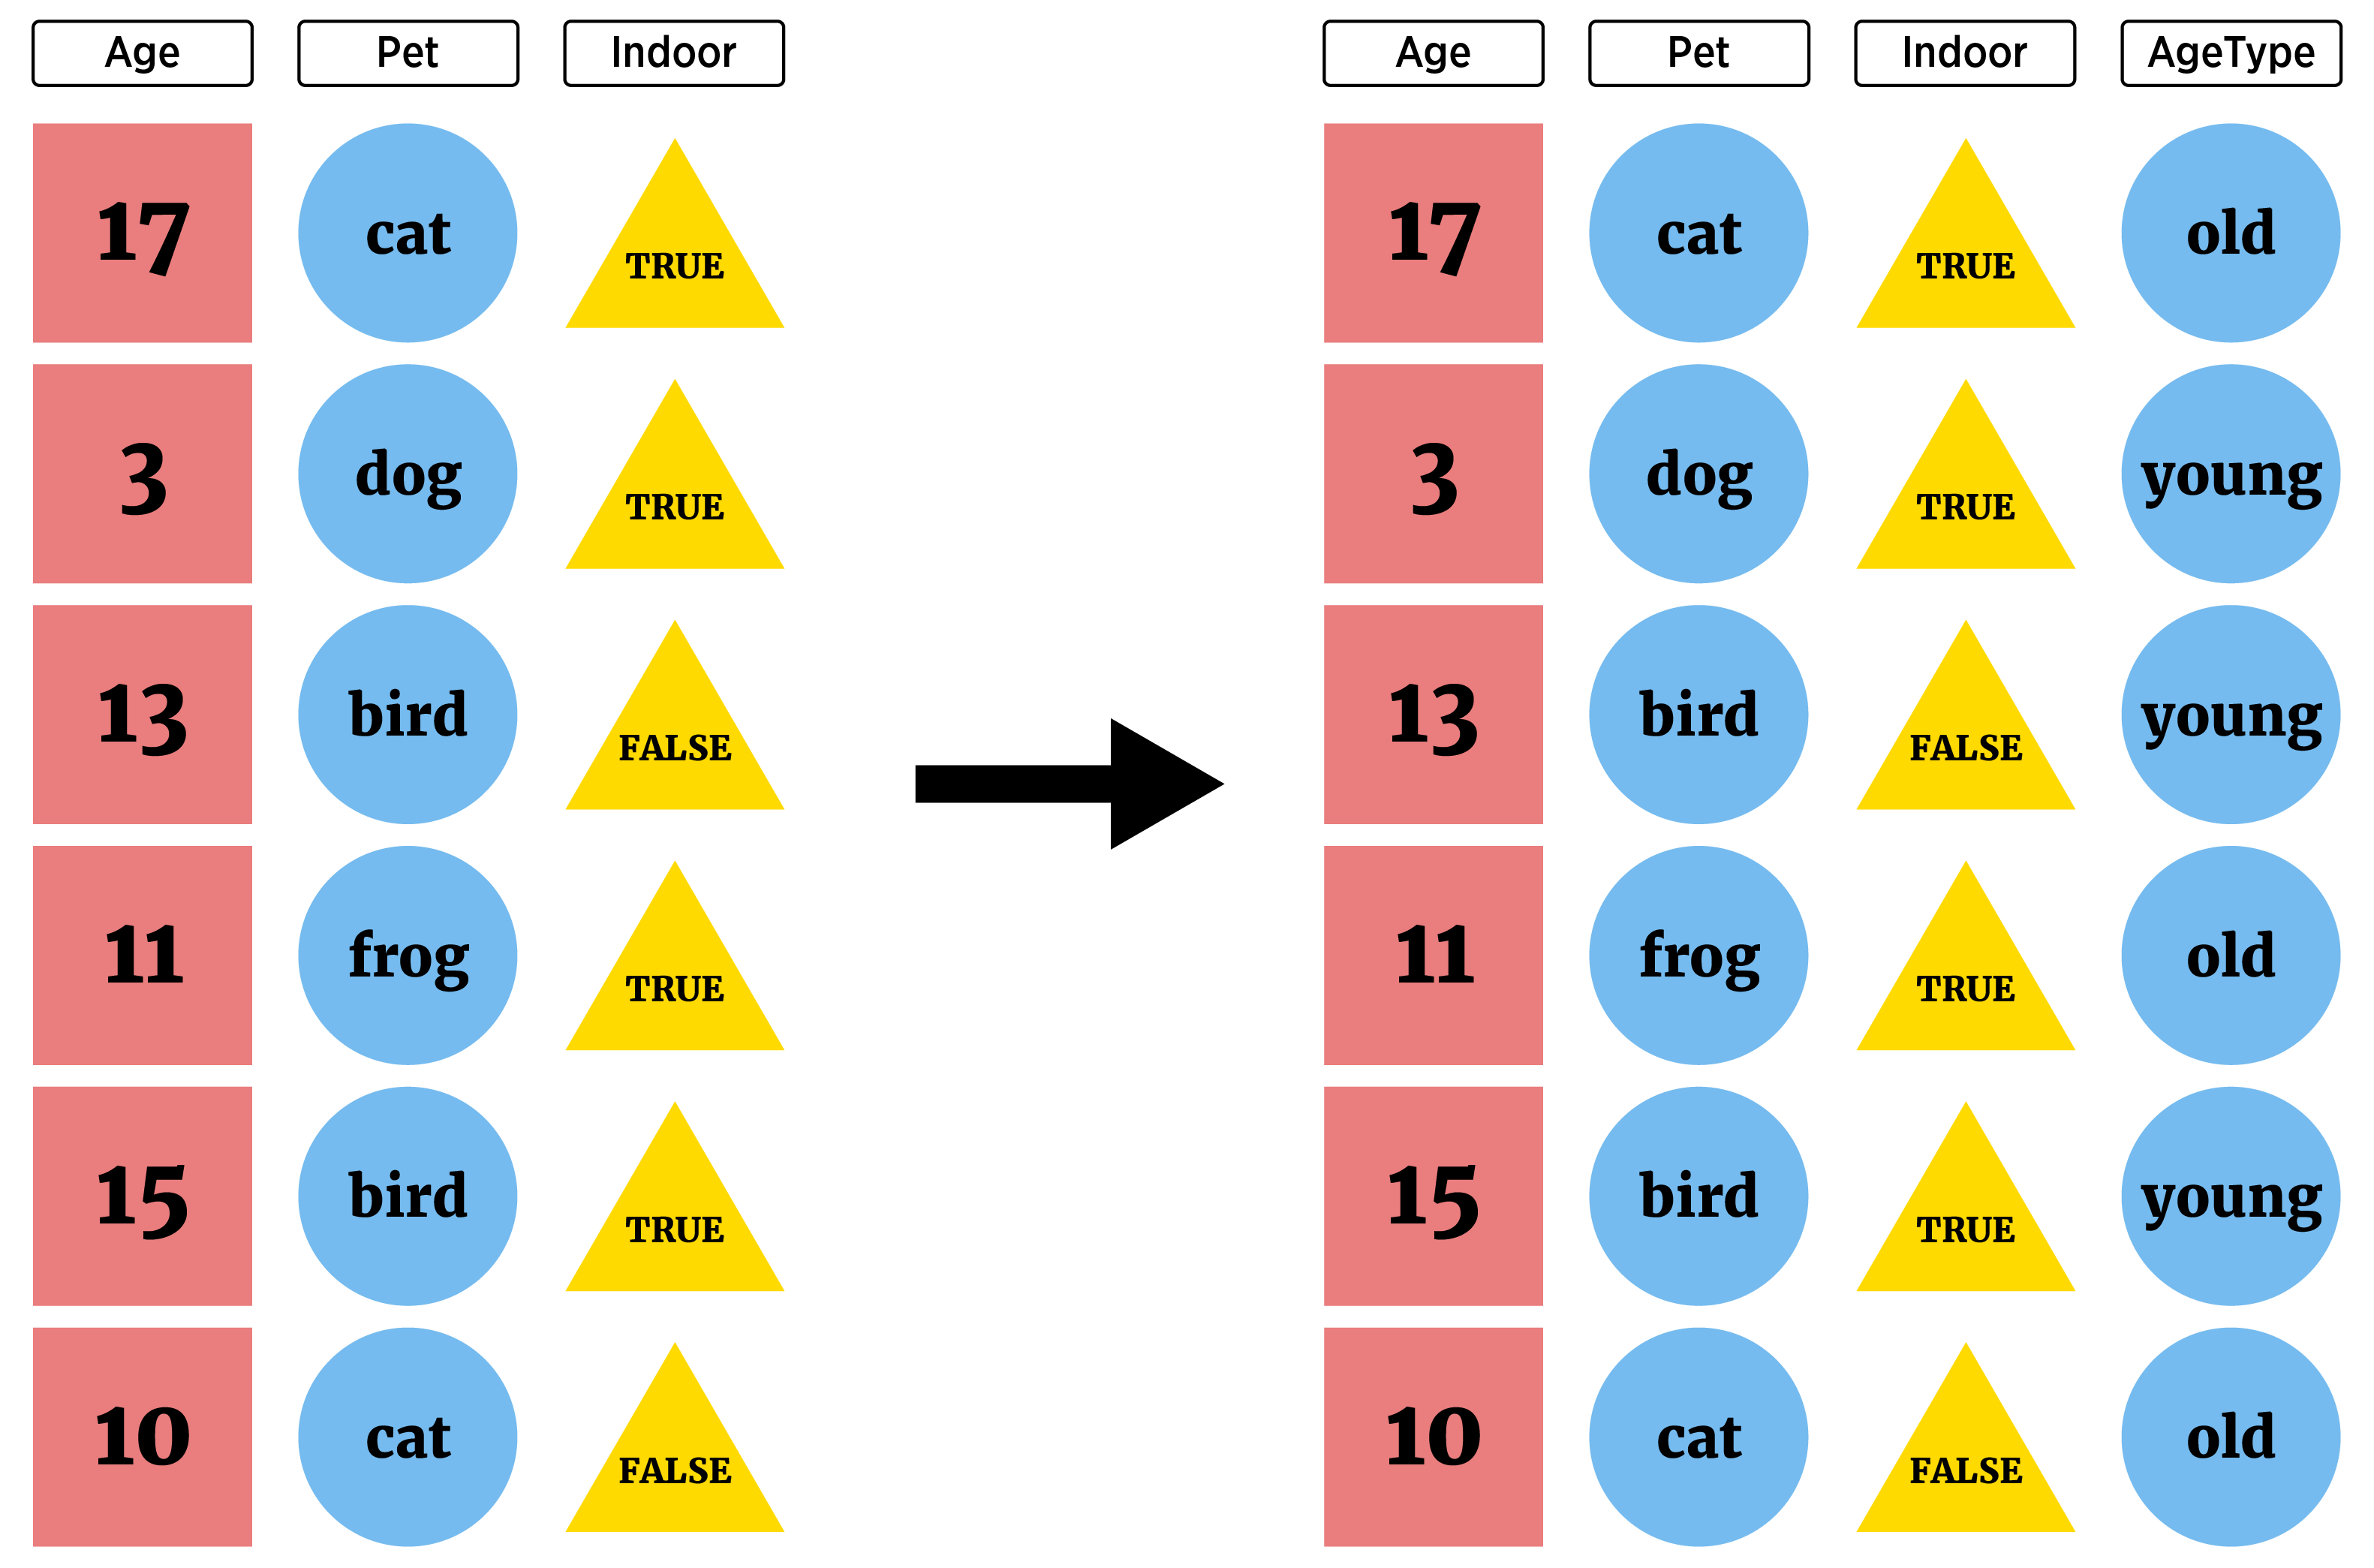
\includegraphics[width=0.8\linewidth]{img/createVarVisualF} \end{center}

When doing data manipulation it is vital to make your work reproducible! Traditionally documentation has been done through comments (\texttt{\#} in R) in your R script. This is being replaced by using a `Notebook' environment like R Markdown.

\hypertarget{documenting-with-markdown-1}{%
\subsection{Documenting with Markdown}\label{documenting-with-markdown-1}}

You may have heard of \href{http://jupyter.org/}{JUPYTER} notebooks. This is a program that allows you to weave plain text with formatting characters along side code. JUPYTER allows you to call Julia, Python, R, or SAS code (among others).

R Markdown is a built in notebook for R studio! A nice intro video is \href{https://vimeo.com/178485416}{available here}.

R Markdown is designed to be used in three ways (R for Data Science):

\begin{itemize}
\item
  Communicating to decision makers (focus on conclusions not code)
\item
  Collaborating with other data scientists (including future you!)
\item
  As environment to do data science (documents what you did and what you were thinking)
\end{itemize}

Most have heard of HTML or HyperText Mark-up Language. This is really just plain text that a web browser like firefox interprets and renders. Markdown is a specific markup language that has easier syntax but is not as powerful. Any plain text file can be used although the .Rmd extension associates the file with R Studio.

RStudio makes it easy to create a Markdown document.

\begin{center}\includegraphics[width=0.75\linewidth]{img/startMD} \end{center}

You can create many commonly used types of output including HTML, PDF, Word, and HTML slides.

\begin{center}\includegraphics[width=0.65\linewidth]{img/startMDDoc} \end{center}

An R Markdown file contains three important types of content:

\begin{enumerate}
\def\labelenumi{\arabic{enumi}.}
\item
  (Optional) YAML header surrounded by \texttt{-\/-\/-}s
\item
  Chunks of R code
\item
  Text mixed with simple text formatting instructions
\end{enumerate}

The YAML header defines settings for document:

\begin{verbatim}
---
title: "Untitled"
author: "First Last"
date: "xxxx"
output: html_document
---
\end{verbatim}

The hot key combination of CTRL/CMD + Shift + k `knits' (or creates the output type) via this information.

Code Chunks can contain any R code. These can be started by typing ```\{r\} out or with CTRL/CMD + Alt + I. This code will be executed when document is created and the chunks will be evaulated sequentially. Options can be specified on individual code chunks to hide their code or output (among other things).

Below you'll see plain text with markdown sytnax included:

\begin{verbatim}
##R Markdown

This is an R Markdown document. Markdown is a simple formatting syntax
for authoring HTML, PDF, and MS Word documents. For more details on
using R Markdown see <http://rmarkdown.rstudio.com>.

When you click the **Knit** button a document will be generated that
includes both content as well as the output of any embedded R code
chunks within the document. 
\end{verbatim}

When the file is created \texttt{\#\#} becomes a header, ``\textless{}\ldots{}\textgreater{}'' a link, and \texttt{**Knit**} bold font.

You can learn much more about how to use R Markdown with this handy \href{https://www.rstudio.com/wp-content/uploads/2015/03/rmarkdown-reference.pdf}{cheat sheet}.

The key idea here is that you can easily write down your thought process and document all of the changes you make to your data. This creates a reproducible final product!

\hypertarget{logical-statements-1}{%
\subsection{Logical Statements}\label{logical-statements-1}}

Our current goal is to subset rows or columns of a dataset.

\begin{center}\includegraphics[width=0.8\linewidth]{img/filterVisualF} \end{center}

To do this efficiently we need to learn about logical statements. A logical statement is a comparison that resolves as \texttt{TRUE} or \texttt{FALSE}. R has all of the standard comparison operators:

\begin{itemize}
\tightlist
\item
  \texttt{==} equal to
\item
  \texttt{!=} not equal to
\item
  \texttt{\textless{}}, \texttt{\textless{}=}, \texttt{\textgreater{}}, \texttt{\textgreater{}=} less than (or equal) and greater than (or equal)
\end{itemize}

\begin{Shaded}
\begin{Highlighting}[]
\StringTok{"hi"} \OperatorTok{==}\StringTok{ " hi"} \CommentTok{#== is comparison}
\end{Highlighting}
\end{Shaded}

\begin{verbatim}
## [1] FALSE
\end{verbatim}

\begin{Shaded}
\begin{Highlighting}[]
\StringTok{"hi"} \OperatorTok{==}\StringTok{ "hi"}
\end{Highlighting}
\end{Shaded}

\begin{verbatim}
## [1] TRUE
\end{verbatim}

\begin{Shaded}
\begin{Highlighting}[]
\DecValTok{4} \OperatorTok{>=}\StringTok{ }\DecValTok{1}
\end{Highlighting}
\end{Shaded}

\begin{verbatim}
## [1] TRUE
\end{verbatim}

\begin{Shaded}
\begin{Highlighting}[]
\DecValTok{4} \OperatorTok{!=}\StringTok{ }\DecValTok{1}
\end{Highlighting}
\end{Shaded}

\begin{verbatim}
## [1] TRUE
\end{verbatim}

Sometimes we see issues due to a loss of precision when doing mathematical operations.

\begin{Shaded}
\begin{Highlighting}[]
\KeywordTok{sqrt}\NormalTok{(}\DecValTok{3}\NormalTok{)}\OperatorTok{^}\DecValTok{2}  \OperatorTok{==}\StringTok{ }\DecValTok{3}
\end{Highlighting}
\end{Shaded}

\begin{verbatim}
## [1] FALSE
\end{verbatim}

The \texttt{near} function from the \texttt{dplyr} package can help with this type of situation.

\begin{Shaded}
\begin{Highlighting}[]
\NormalTok{dplyr}\OperatorTok{::}\KeywordTok{near}\NormalTok{(}\KeywordTok{sqrt}\NormalTok{(}\DecValTok{3}\NormalTok{)}\OperatorTok{^}\DecValTok{2}\NormalTok{, }\DecValTok{3}\NormalTok{)}
\end{Highlighting}
\end{Shaded}

\begin{verbatim}
## [1] TRUE
\end{verbatim}

Another common way to do a logical statement in R is to use an \texttt{is.} family function.

\begin{Shaded}
\begin{Highlighting}[]
\KeywordTok{is.numeric}\NormalTok{(}\StringTok{"Word"}\NormalTok{)}
\end{Highlighting}
\end{Shaded}

\begin{verbatim}
## [1] FALSE
\end{verbatim}

\begin{Shaded}
\begin{Highlighting}[]
\KeywordTok{is.numeric}\NormalTok{(}\DecValTok{10}\NormalTok{)}
\end{Highlighting}
\end{Shaded}

\begin{verbatim}
## [1] TRUE
\end{verbatim}

\begin{Shaded}
\begin{Highlighting}[]
\KeywordTok{is.character}\NormalTok{(}\StringTok{"10"}\NormalTok{)}
\end{Highlighting}
\end{Shaded}

\begin{verbatim}
## [1] TRUE
\end{verbatim}

\begin{Shaded}
\begin{Highlighting}[]
\KeywordTok{is.na}\NormalTok{(}\KeywordTok{c}\NormalTok{(}\DecValTok{1}\OperatorTok{:}\DecValTok{2}\NormalTok{, }\OtherTok{NA}\NormalTok{, }\DecValTok{3}\NormalTok{))}
\end{Highlighting}
\end{Shaded}

\begin{verbatim}
## [1] FALSE FALSE  TRUE FALSE
\end{verbatim}

\begin{Shaded}
\begin{Highlighting}[]
\KeywordTok{is.matrix}\NormalTok{(}\KeywordTok{c}\NormalTok{(}\StringTok{"hello"}\NormalTok{, }\StringTok{"world"}\NormalTok{))}
\end{Highlighting}
\end{Shaded}

\begin{verbatim}
## [1] FALSE
\end{verbatim}

How do we use logical statements to subset our data? Logical vectors can be used for indexing an R object. The concept is:

\begin{itemize}
\tightlist
\item
  Feed index a vector of \texttt{TRUE}/\texttt{FALSE} or \texttt{0}/\texttt{1} values\\
\item
  R will return elements where \texttt{TRUE} or \texttt{1} occurred
\end{itemize}

Let's subset the built-in \texttt{iris} data set. First we'll convert it to a \texttt{tibble} so it prints nicely.

\begin{Shaded}
\begin{Highlighting}[]
\NormalTok{iris <-}\StringTok{ }\KeywordTok{tbl_df}\NormalTok{(iris)}
\NormalTok{iris}
\end{Highlighting}
\end{Shaded}

Now, we can create an indexing vector corresponding to some condition of interest. For instance, we may want to only look at the Species `setosa' flowers.

\begin{Shaded}
\begin{Highlighting}[]
\NormalTok{iris}\OperatorTok{$}\NormalTok{Species }\OperatorTok{==}\StringTok{ "setosa"} \CommentTok{#vector indicating setosa values}
\end{Highlighting}
\end{Shaded}

\begin{verbatim}
##   [1]  TRUE  TRUE  TRUE  TRUE  TRUE  TRUE  TRUE  TRUE  TRUE  TRUE  TRUE  TRUE
##  [13]  TRUE  TRUE  TRUE  TRUE  TRUE  TRUE  TRUE  TRUE  TRUE  TRUE  TRUE  TRUE
##  [25]  TRUE  TRUE  TRUE  TRUE  TRUE  TRUE  TRUE  TRUE  TRUE  TRUE  TRUE  TRUE
##  [37]  TRUE  TRUE  TRUE  TRUE  TRUE  TRUE  TRUE  TRUE  TRUE  TRUE  TRUE  TRUE
##  [49]  TRUE  TRUE FALSE FALSE FALSE FALSE FALSE FALSE FALSE FALSE FALSE FALSE
##  [61] FALSE FALSE FALSE FALSE FALSE FALSE FALSE FALSE FALSE FALSE FALSE FALSE
##  [73] FALSE FALSE FALSE FALSE FALSE FALSE FALSE FALSE FALSE FALSE FALSE FALSE
##  [85] FALSE FALSE FALSE FALSE FALSE FALSE FALSE FALSE FALSE FALSE FALSE FALSE
##  [97] FALSE FALSE FALSE FALSE
##  [ reached getOption("max.print") -- omitted 50 entries ]
\end{verbatim}

Now we can feed this in as our row index to the \texttt{{[}} function. Remember for rectangular data the first index you give refers to the rows and the second to columns.

\begin{Shaded}
\begin{Highlighting}[]
\NormalTok{iris[iris}\OperatorTok{$}\NormalTok{Species }\OperatorTok{==}\StringTok{ "setosa"}\NormalTok{, ]}
\end{Highlighting}
\end{Shaded}

\begin{verbatim}
##    Sepal.Length Sepal.Width Petal.Length Petal.Width Species extra
## 1           5.1         3.5          1.4         0.2  setosa     a
## 2           4.9         3.0          1.4         0.2  setosa     a
## 3           4.7         3.2          1.3         0.2  setosa     a
## 4           4.6         3.1          1.5         0.2  setosa     a
## 5           5.0         3.6          1.4         0.2  setosa     a
## 6           5.4         3.9          1.7         0.4  setosa     a
## 7           4.6         3.4          1.4         0.3  setosa     a
## 8           5.0         3.4          1.5         0.2  setosa     a
## 9           4.4         2.9          1.4         0.2  setosa     a
## 10          4.9         3.1          1.5         0.1  setosa     a
## 11          5.4         3.7          1.5         0.2  setosa     a
## 12          4.8         3.4          1.6         0.2  setosa     a
## 13          4.8         3.0          1.4         0.1  setosa     a
## 14          4.3         3.0          1.1         0.1  setosa     a
## 15          5.8         4.0          1.2         0.2  setosa     a
## 16          5.7         4.4          1.5         0.4  setosa     a
##  [ reached 'max' / getOption("max.print") -- omitted 34 rows ]
\end{verbatim}

Rather than use \texttt{{[}}, a base R function called \texttt{subset} can be used.

\begin{Shaded}
\begin{Highlighting}[]
\KeywordTok{subset}\NormalTok{(iris, Species }\OperatorTok{==}\StringTok{ "setosa"}\NormalTok{)}
\end{Highlighting}
\end{Shaded}

\begin{verbatim}
##    Sepal.Length Sepal.Width Petal.Length Petal.Width Species extra
## 1           5.1         3.5          1.4         0.2  setosa     a
## 2           4.9         3.0          1.4         0.2  setosa     a
## 3           4.7         3.2          1.3         0.2  setosa     a
## 4           4.6         3.1          1.5         0.2  setosa     a
## 5           5.0         3.6          1.4         0.2  setosa     a
## 6           5.4         3.9          1.7         0.4  setosa     a
## 7           4.6         3.4          1.4         0.3  setosa     a
## 8           5.0         3.4          1.5         0.2  setosa     a
## 9           4.4         2.9          1.4         0.2  setosa     a
## 10          4.9         3.1          1.5         0.1  setosa     a
## 11          5.4         3.7          1.5         0.2  setosa     a
## 12          4.8         3.4          1.6         0.2  setosa     a
## 13          4.8         3.0          1.4         0.1  setosa     a
## 14          4.3         3.0          1.1         0.1  setosa     a
## 15          5.8         4.0          1.2         0.2  setosa     a
## 16          5.7         4.4          1.5         0.4  setosa     a
##  [ reached 'max' / getOption("max.print") -- omitted 34 rows ]
\end{verbatim}

This function works quite well but we want to work in the tidyverse. The \texttt{filter} function from the \texttt{dplyr} package (installed with \texttt{tidyverse}) will be our function of choice. For \texttt{filter} the first argument is the data frame (or tibble) and the second is the logical statement used for indexing the rows.

\begin{Shaded}
\begin{Highlighting}[]
\KeywordTok{filter}\NormalTok{(iris, Species }\OperatorTok{==}\StringTok{ "setosa"}\NormalTok{)}
\end{Highlighting}
\end{Shaded}

\begin{verbatim}
##    Sepal.Length Sepal.Width Petal.Length Petal.Width Species extra
## 1           5.1         3.5          1.4         0.2  setosa     a
## 2           4.9         3.0          1.4         0.2  setosa     a
## 3           4.7         3.2          1.3         0.2  setosa     a
## 4           4.6         3.1          1.5         0.2  setosa     a
## 5           5.0         3.6          1.4         0.2  setosa     a
## 6           5.4         3.9          1.7         0.4  setosa     a
## 7           4.6         3.4          1.4         0.3  setosa     a
## 8           5.0         3.4          1.5         0.2  setosa     a
## 9           4.4         2.9          1.4         0.2  setosa     a
## 10          4.9         3.1          1.5         0.1  setosa     a
## 11          5.4         3.7          1.5         0.2  setosa     a
## 12          4.8         3.4          1.6         0.2  setosa     a
## 13          4.8         3.0          1.4         0.1  setosa     a
## 14          4.3         3.0          1.1         0.1  setosa     a
## 15          5.8         4.0          1.2         0.2  setosa     a
## 16          5.7         4.4          1.5         0.4  setosa     a
##  [ reached 'max' / getOption("max.print") -- omitted 34 rows ]
\end{verbatim}

Often we'll want to subset based on more than one condition. These can be created using standard logical operators. In R these are:

\begin{itemize}
\tightlist
\item
  \texttt{\&} `and'
\item
  \texttt{\textbar{}} `or'
\end{itemize}

\begin{longtable}[]{@{}llll@{}}
\toprule
Operator & A,B true & A true, B false & A,B false\tabularnewline
\midrule
\endhead
\texttt{\&} & \texttt{A\ \&\ B\ =\ TRUE} & \texttt{A\ \&\ B\ =\ FALSE} & \texttt{A\ \&\ B\ =\ FALSE}\tabularnewline
\texttt{\textbar{}} & \texttt{A\ \textbar{}\ B\ =\ TRUE} & \texttt{A\ \textbar{}\ B\ =\ TRUE} & \texttt{A\ \textbar{}\ B\ =\ FALSE}\tabularnewline
\bottomrule
\end{longtable}

For the most part we'll want to use the single \texttt{\&} or \texttt{\textbar{}}. \texttt{\&\&} and \texttt{\textbar{}\textbar{}} are alternatives that only look at only first comparison done (if given a vector of comparisons).

A quick example of the compound logical syntax is given below. Parenthesis are not necessary but are quite useful to keep things straight! Here we generate 10 random values between 0 and 1 (\texttt{set.seed} just starts the random number generator at a specific spot so we can get the same 10 values each time we create this document!). We use \texttt{\textbar{}} to return TRUE if the randomly generated value is either below 0.25 or above 0.75.

\begin{Shaded}
\begin{Highlighting}[]
\KeywordTok{set.seed}\NormalTok{(}\DecValTok{3}\NormalTok{)}
\NormalTok{x <-}\StringTok{ }\KeywordTok{runif}\NormalTok{(}\DataTypeTok{n =} \DecValTok{10}\NormalTok{, }\DataTypeTok{min =} \DecValTok{0}\NormalTok{, }\DataTypeTok{max =} \DecValTok{1}\NormalTok{)}
\NormalTok{x}
\end{Highlighting}
\end{Shaded}

\begin{verbatim}
##  [1] 0.1680415 0.8075164 0.3849424 0.3277343 0.6021007 0.6043941 0.1246334
##  [8] 0.2946009 0.5776099 0.6309793
\end{verbatim}

\begin{Shaded}
\begin{Highlighting}[]
\NormalTok{(x }\OperatorTok{<}\StringTok{ }\FloatTok{0.25}\NormalTok{) }\OperatorTok{|}\StringTok{ }\NormalTok{(x }\OperatorTok{>}\StringTok{ }\FloatTok{0.75}\NormalTok{)}
\end{Highlighting}
\end{Shaded}

\begin{verbatim}
##  [1]  TRUE  TRUE FALSE FALSE FALSE FALSE  TRUE FALSE FALSE FALSE
\end{verbatim}

With this kind of syntax we can now create an indexing vector to only pull out large petal setosa flowers:

\begin{Shaded}
\begin{Highlighting}[]
\NormalTok{(iris}\OperatorTok{$}\NormalTok{Petal.Length }\OperatorTok{>}\StringTok{ }\FloatTok{1.5}\NormalTok{) }\OperatorTok{&}\StringTok{ }\NormalTok{(iris}\OperatorTok{$}\NormalTok{Petal.Width }\OperatorTok{>}\StringTok{ }\FloatTok{0.3}\NormalTok{) }\OperatorTok{&}\StringTok{ }\NormalTok{(iris}\OperatorTok{$}\NormalTok{Species }\OperatorTok{==}\StringTok{ "setosa"}\NormalTok{)}
\end{Highlighting}
\end{Shaded}

\begin{verbatim}
##   [1] FALSE FALSE FALSE FALSE FALSE  TRUE FALSE FALSE FALSE FALSE FALSE FALSE
##  [13] FALSE FALSE FALSE FALSE FALSE FALSE FALSE FALSE FALSE FALSE FALSE  TRUE
##  [25] FALSE FALSE  TRUE FALSE FALSE FALSE FALSE FALSE FALSE FALSE FALSE FALSE
##  [37] FALSE FALSE FALSE FALSE FALSE FALSE FALSE  TRUE  TRUE FALSE FALSE FALSE
##  [49] FALSE FALSE FALSE FALSE FALSE FALSE FALSE FALSE FALSE FALSE FALSE FALSE
##  [61] FALSE FALSE FALSE FALSE FALSE FALSE FALSE FALSE FALSE FALSE FALSE FALSE
##  [73] FALSE FALSE FALSE FALSE FALSE FALSE FALSE FALSE FALSE FALSE FALSE FALSE
##  [85] FALSE FALSE FALSE FALSE FALSE FALSE FALSE FALSE FALSE FALSE FALSE FALSE
##  [97] FALSE FALSE FALSE FALSE
##  [ reached getOption("max.print") -- omitted 50 entries ]
\end{verbatim}

Using this in the filter function we return only a few observations corresponding to our condition.

\begin{Shaded}
\begin{Highlighting}[]
\KeywordTok{filter}\NormalTok{(iris, (Petal.Length }\OperatorTok{>}\StringTok{ }\FloatTok{1.5}\NormalTok{) }\OperatorTok{&}\StringTok{ }\NormalTok{(Petal.Width }\OperatorTok{>}\StringTok{ }\FloatTok{0.3}\NormalTok{) }\OperatorTok{&}\StringTok{ }
\StringTok{         }\NormalTok{(Species }\OperatorTok{==}\StringTok{ "setosa"}\NormalTok{))}
\end{Highlighting}
\end{Shaded}

\begin{verbatim}
##   Sepal.Length Sepal.Width Petal.Length Petal.Width Species extra
## 1          5.4         3.9          1.7         0.4  setosa     a
## 2          5.1         3.3          1.7         0.5  setosa     a
## 3          5.0         3.4          1.6         0.4  setosa     a
## 4          5.0         3.5          1.6         0.6  setosa     a
## 5          5.1         3.8          1.9         0.4  setosa     a
\end{verbatim}

\hypertarget{dplyr-1}{%
\subsection{\texorpdfstring{\texttt{dplyr}}{dplyr}}\label{dplyr-1}}

The tidyverse has many useful packages for common data manipulation tasks. Make sure \texttt{library(tidyverse)} has been run when working through this section!\\
Two major packages for data manipulation are:

-\texttt{dplry} package made for most standard data manipulation tasks

\begin{itemize}
\tightlist
\item
  \texttt{tidyr} package reshapes data (wide and long format, split columns, etc)
\end{itemize}

This section focuses on the most useful functions from the \texttt{dplyr} package:

\begin{itemize}
\tightlist
\item
  \texttt{tbl\_df()} - convert data frame to one with better printing\\
\item
  \texttt{filter()} - subset rows\\
\item
  \texttt{arrange()} - reorder rows\\
\item
  \texttt{select()} - subset columns\\
\item
  \texttt{rename()} - rename columns
\end{itemize}

Later we'll look at

\begin{itemize}
\tightlist
\item
  \texttt{mutate()} - add newly created column\\
\item
  \texttt{transmute()} - create new variable\\
\item
  \texttt{group\_by()} - group rows by a variable\\
\item
  \texttt{summarise()} - apply basic function to data
\end{itemize}

One really nice thing about the functions in the tidyverse is that the syntax is mostly consistent (save \texttt{ggplot2}). The basic syntax is

\texttt{function(tibble,\ actions,\ ...)}

Let's get started! We've seen \texttt{tbl\_df} a few times. This function converts a data frame to one with better printing and no simplification. To use it we can simply `wrap' data frame with it. In this section we'll do examples on datasets from the \texttt{Lahman} pacakge. This package has data about baseball players dating back from the start of professional baseball.

\begin{Shaded}
\begin{Highlighting}[]
\CommentTok{#install.packages("Lahman")}
\KeywordTok{library}\NormalTok{(Lahman)}
\CommentTok{#old method for previewing a dataset}
\KeywordTok{head}\NormalTok{(Batting, }\DataTypeTok{n =} \DecValTok{4}\NormalTok{) }\CommentTok{#look at just first 4 observations}
\end{Highlighting}
\end{Shaded}

\begin{verbatim}
## # A tibble: 4 x 22
##   playerID yearID stint teamID lgID      G    AB     R     H   X2B   X3B    HR
##   <chr>     <int> <int> <fct>  <fct> <int> <int> <int> <int> <int> <int> <int>
## 1 abercda~   1871     1 TRO    NA        1     4     0     0     0     0     0
## 2 addybo01   1871     1 RC1    NA       25   118    30    32     6     0     0
## 3 allisar~   1871     1 CL1    NA       29   137    28    40     4     5     0
## 4 allisdo~   1871     1 WS3    NA       27   133    28    44    10     2     2
## # ... with 10 more variables: RBI <int>, SB <int>, CS <int>, BB <int>,
## #   SO <int>, IBB <int>, HBP <int>, SH <int>, SF <int>, GIDP <int>
\end{verbatim}

\begin{Shaded}
\begin{Highlighting}[]
\NormalTok{Batting <-}\StringTok{ }\KeywordTok{tbl_df}\NormalTok{(Batting)}
\NormalTok{Batting}
\end{Highlighting}
\end{Shaded}

\begin{verbatim}
## # A tibble: 105,861 x 22
##   playerID yearID stint teamID lgID      G    AB     R     H   X2B   X3B    HR
##   <chr>     <int> <int> <fct>  <fct> <int> <int> <int> <int> <int> <int> <int>
## 1 abercda~   1871     1 TRO    NA        1     4     0     0     0     0     0
## 2 addybo01   1871     1 RC1    NA       25   118    30    32     6     0     0
## 3 allisar~   1871     1 CL1    NA       29   137    28    40     4     5     0
## 4 allisdo~   1871     1 WS3    NA       27   133    28    44    10     2     2
## 5 ansonca~   1871     1 RC1    NA       25   120    29    39    11     3     0
## # ... with 1.059e+05 more rows, and 10 more variables: RBI <int>, SB <int>,
## #   CS <int>, BB <int>, SO <int>, IBB <int>, HBP <int>, SH <int>, SF <int>,
## #   GIDP <int>
\end{verbatim}

If the data has been read in with \texttt{haven}, \texttt{readxl}, or \texttt{readr}, it is probably in this format already!

\hypertarget{row-manipulations-1}{%
\subsubsection{Row Manipulations}\label{row-manipulations-1}}

Again, we may to do a subset based on the rows of our dataset.

\begin{center}\includegraphics[width=0.8\linewidth]{img/filterVisualF} \end{center}

We just looked at using the \texttt{filter} function to subset rows or observations of a dataset. Let's look at a few more examples. We may only want to return observations from the Batting dataset corresponding to the Pittsburgh Pirates (PIT).

\begin{Shaded}
\begin{Highlighting}[]
\KeywordTok{filter}\NormalTok{(Batting, teamID }\OperatorTok{==}\StringTok{ "PIT"}\NormalTok{)}
\end{Highlighting}
\end{Shaded}

\begin{verbatim}
## # A tibble: 4,817 x 22
##   playerID yearID stint teamID lgID      G    AB     R     H   X2B   X3B    HR
##   <chr>     <int> <int> <fct>  <fct> <int> <int> <int> <int> <int> <int> <int>
## 1 barklsa~   1887     1 PIT    NL       89   340    44    76    10     4     1
## 2 beeched~   1887     1 PIT    NL       41   169    15    41     8     0     2
## 3 bishobi~   1887     1 PIT    NL        3     9     0     0     0     0     0
## 4 brownto~   1887     1 PIT    NL       47   192    30    47     3     4     0
## 5 carrofr~   1887     1 PIT    NL      102   421    71   138    24    15     6
## # ... with 4,812 more rows, and 10 more variables: RBI <int>, SB <int>,
## #   CS <int>, BB <int>, SO <int>, IBB <int>, HBP <int>, SH <int>, SF <int>,
## #   GIDP <int>
\end{verbatim}

We could use a compound logical to only return Pirate data from the year 2000.

\begin{Shaded}
\begin{Highlighting}[]
\KeywordTok{filter}\NormalTok{(Batting, teamID }\OperatorTok{==}\StringTok{ "PIT"} \OperatorTok{&}\StringTok{ }\NormalTok{yearID }\OperatorTok{==}\StringTok{ }\DecValTok{2000}\NormalTok{)}
\end{Highlighting}
\end{Shaded}

\begin{verbatim}
## # A tibble: 46 x 22
##   playerID yearID stint teamID lgID      G    AB     R     H   X2B   X3B    HR
##   <chr>     <int> <int> <fct>  <fct> <int> <int> <int> <int> <int> <int> <int>
## 1 anderji~   2000     1 PIT    NL       27    50     5     7     1     0     0
## 2 arroybr~   2000     1 PIT    NL       21    21     2     3     2     0     0
## 3 avenbr01   2000     1 PIT    NL       72   148    18    37    11     0     5
## 4 benjami~   2000     1 PIT    NL       93   233    28    63    18     2     2
## 5 bensokr~   2000     1 PIT    NL       32    65     3     6     2     0     0
## # ... with 41 more rows, and 10 more variables: RBI <int>, SB <int>, CS <int>,
## #   BB <int>, SO <int>, IBB <int>, HBP <int>, SH <int>, SF <int>, GIDP <int>
\end{verbatim}

Another useful row operation is to rearrange the data based on some criteria. The \texttt{arrange} function allows us to sort a data set by numeric or character variables. For instance we could reorder alphabetically by the teamID variable.

\begin{Shaded}
\begin{Highlighting}[]
\KeywordTok{arrange}\NormalTok{(Batting, teamID)}
\end{Highlighting}
\end{Shaded}

\begin{verbatim}
## # A tibble: 105,861 x 22
##   playerID yearID stint teamID lgID      G    AB     R     H   X2B   X3B    HR
##   <chr>     <int> <int> <fct>  <fct> <int> <int> <int> <int> <int> <int> <int>
## 1 berrych~   1884     1 ALT    UA        7    25     2     6     0     0     0
## 2 brownji~   1884     1 ALT    UA       21    88    12    22     2     2     1
## 3 carropa~   1884     1 ALT    UA       11    49     4    13     1     0     0
## 4 connojo~   1884     1 ALT    UA        3    11     0     1     0     0     0
## 5 crosscl~   1884     1 ALT    UA        2     7     1     4     1     0     0
## # ... with 1.059e+05 more rows, and 10 more variables: RBI <int>, SB <int>,
## #   CS <int>, BB <int>, SO <int>, IBB <int>, HBP <int>, SH <int>, SF <int>,
## #   GIDP <int>
\end{verbatim}

A secondary arrangement can be done as well (and third, etc.)

\begin{Shaded}
\begin{Highlighting}[]
\KeywordTok{arrange}\NormalTok{(Batting, teamID, G)}
\end{Highlighting}
\end{Shaded}

\begin{verbatim}
## # A tibble: 105,861 x 22
##   playerID yearID stint teamID lgID      G    AB     R     H   X2B   X3B    HR
##   <chr>     <int> <int> <fct>  <fct> <int> <int> <int> <int> <int> <int> <int>
## 1 daisege~   1884     1 ALT    UA        1     4     0     0     0     0     0
## 2 crosscl~   1884     1 ALT    UA        2     7     1     4     1     0     0
## 3 manloch~   1884     1 ALT    UA        2     7     1     3     0     0     0
## 4 connojo~   1884     1 ALT    UA        3    11     0     1     0     0     0
## 5 shafff01   1884     1 ALT    UA        6    19     1     3     0     0     0
## # ... with 1.059e+05 more rows, and 10 more variables: RBI <int>, SB <int>,
## #   CS <int>, BB <int>, SO <int>, IBB <int>, HBP <int>, SH <int>, SF <int>,
## #   GIDP <int>
\end{verbatim}

The arrangement can be done descending as well by giving the column (variable) with \texttt{desc}.

\begin{Shaded}
\begin{Highlighting}[]
\KeywordTok{arrange}\NormalTok{(Batting, teamID, }\KeywordTok{desc}\NormalTok{(G))}
\end{Highlighting}
\end{Shaded}

\begin{verbatim}
## # A tibble: 105,861 x 22
##   playerID yearID stint teamID lgID      G    AB     R     H   X2B   X3B    HR
##   <chr>     <int> <int> <fct>  <fct> <int> <int> <int> <int> <int> <int> <int>
## 1 smithge~   1884     1 ALT    UA       25   108     9    34     8     1     0
## 2 harrifr~   1884     1 ALT    UA       24    95    10    25     2     1     0
## 3 doughch~   1884     1 ALT    UA       23    85     6    22     5     0     0
## 4 murphjo~   1884     1 ALT    UA       23    94    10    14     1     0     0
## 5 brownji~   1884     1 ALT    UA       21    88    12    22     2     2     1
## # ... with 1.059e+05 more rows, and 10 more variables: RBI <int>, SB <int>,
## #   CS <int>, BB <int>, SO <int>, IBB <int>, HBP <int>, SH <int>, SF <int>,
## #   GIDP <int>
\end{verbatim}

\hypertarget{column-manipulations-1}{%
\subsubsection{Column Manipulations}\label{column-manipulations-1}}

We may want to look at only certain variables (select columns).

\begin{center}\includegraphics[width=0.65\linewidth]{img/selectVisualF} \end{center}

The \texttt{select} function from the \texttt{dplyr} package allows us to choose columns of interest. We've seen the use of \texttt{\$} and \texttt{{[}\ ,\ {]}} to do this already but \texttt{select} offers many advantages.

\begin{itemize}
\item
  Same syntax as tidyverse functions
\item
  Useful ways to use character matching to select columns
\end{itemize}

Let's see it in action! To choose a single column of interest just supply the column name (or position) after the \texttt{tibble}.

\begin{Shaded}
\begin{Highlighting}[]
\KeywordTok{select}\NormalTok{(Batting, X2B)}
\end{Highlighting}
\end{Shaded}

\begin{verbatim}
## # A tibble: 105,861 x 1
##     X2B
##   <int>
## 1     0
## 2     6
## 3     4
## 4    10
## 5    11
## # ... with 1.059e+05 more rows
\end{verbatim}

Multiple columns can be selected by giving multiple column names.

\begin{Shaded}
\begin{Highlighting}[]
\KeywordTok{select}\NormalTok{(Batting, playerID, X2B)}
\end{Highlighting}
\end{Shaded}

\begin{verbatim}
## # A tibble: 105,861 x 2
##   playerID    X2B
##   <chr>     <int>
## 1 abercda01     0
## 2 addybo01      6
## 3 allisar01     4
## 4 allisdo01    10
## 5 ansonca01    11
## # ... with 1.059e+05 more rows
\end{verbatim}

There are many ways to select multiple columsn (variables). For instance, contiguous columns can be selected using the \texttt{:}.

\begin{Shaded}
\begin{Highlighting}[]
\CommentTok{#all columns between}
\KeywordTok{select}\NormalTok{(Batting, X2B}\OperatorTok{:}\NormalTok{HR)}
\end{Highlighting}
\end{Shaded}

\begin{verbatim}
## # A tibble: 105,861 x 3
##     X2B   X3B    HR
##   <int> <int> <int>
## 1     0     0     0
## 2     6     0     0
## 3     4     5     0
## 4    10     2     2
## 5    11     3     0
## # ... with 1.059e+05 more rows
\end{verbatim}

Character matching can be done to select all columns that contain a certain character.

\begin{Shaded}
\begin{Highlighting}[]
\CommentTok{#all columns containing}
\KeywordTok{select}\NormalTok{(Batting, }\KeywordTok{contains}\NormalTok{(}\StringTok{"X"}\NormalTok{))}
\end{Highlighting}
\end{Shaded}

\begin{verbatim}
## # A tibble: 105,861 x 2
##     X2B   X3B
##   <int> <int>
## 1     0     0
## 2     6     0
## 3     4     5
## 4    10     2
## 5    11     3
## # ... with 1.059e+05 more rows
\end{verbatim}

Similary, there is a \texttt{starts\_with} and \texttt{ends\_with} function.

\begin{Shaded}
\begin{Highlighting}[]
\CommentTok{#all columns starting with}
\KeywordTok{select}\NormalTok{(Batting, }\KeywordTok{starts_with}\NormalTok{(}\StringTok{"X"}\NormalTok{))}
\end{Highlighting}
\end{Shaded}

\begin{verbatim}
## # A tibble: 105,861 x 2
##     X2B   X3B
##   <int> <int>
## 1     0     0
## 2     6     0
## 3     4     5
## 4    10     2
## 5    11     3
## # ... with 1.059e+05 more rows
\end{verbatim}

\begin{Shaded}
\begin{Highlighting}[]
\CommentTok{#multiple selections}
\KeywordTok{select}\NormalTok{(Batting, }\KeywordTok{starts_with}\NormalTok{(}\StringTok{"X"}\NormalTok{), }\KeywordTok{ends_with}\NormalTok{(}\StringTok{"ID"}\NormalTok{), G)}
\end{Highlighting}
\end{Shaded}

\begin{verbatim}
## # A tibble: 105,861 x 7
##     X2B   X3B playerID  yearID teamID lgID      G
##   <int> <int> <chr>      <int> <fct>  <fct> <int>
## 1     0     0 abercda01   1871 TRO    NA        1
## 2     6     0 addybo01    1871 RC1    NA       25
## 3     4     5 allisar01   1871 CL1    NA       29
## 4    10     2 allisdo01   1871 WS3    NA       27
## 5    11     3 ansonca01   1871 RC1    NA       25
## # ... with 1.059e+05 more rows
\end{verbatim}

Sometimes we want to rename variables. This can be done with the \texttt{rename} function.

\begin{Shaded}
\begin{Highlighting}[]
\CommentTok{#rename our previous selection}
\KeywordTok{rename}\NormalTok{(}\KeywordTok{select}\NormalTok{(Batting, }\KeywordTok{starts_with}\NormalTok{(}\StringTok{"X"}\NormalTok{), }\KeywordTok{ends_with}\NormalTok{(}\StringTok{"ID"}\NormalTok{), G), }\StringTok{"Doubles"}\NormalTok{ =}\StringTok{ }\NormalTok{X2B, }\StringTok{"Triples"}\NormalTok{ =}\StringTok{ }\NormalTok{X3B)}
\end{Highlighting}
\end{Shaded}

\begin{verbatim}
## # A tibble: 105,861 x 7
##   Doubles Triples playerID  yearID teamID lgID      G
##     <int>   <int> <chr>      <int> <fct>  <fct> <int>
## 1       0       0 abercda01   1871 TRO    NA        1
## 2       6       0 addybo01    1871 RC1    NA       25
## 3       4       5 allisar01   1871 CL1    NA       29
## 4      10       2 allisdo01   1871 WS3    NA       27
## 5      11       3 ansonca01   1871 RC1    NA       25
## # ... with 1.059e+05 more rows
\end{verbatim}

You may notice this is kind function nesting makes this code difficult for humans to parse. Piping or Chaining can be used to make the use of multiple functions easier!

\texttt{\%\textgreater{}\%} is the piping operator. Generically, piping does the following

\texttt{x\ \%\textgreater{}\%\ f(y)} turns into \texttt{f(x,y)}

\texttt{x\ \%\textgreater{}\%\ f(y)\ \%\textgreater{}\%\ g(z)} turns into \texttt{g(f(x,\ y),\ z)}

Since the tidyverse functions all have the same syntax, piping works wonders for readability! Piping can be used with functions outside the tidyverse if this structure works. Let's rewrite our previous nested function with piping. When reading code with piping, read \texttt{\%\textgreater{}\%} as the word `then.'

Batting data set (then) select these columns (then) rename the variables.

\begin{Shaded}
\begin{Highlighting}[]
\NormalTok{Batting }\OperatorTok\StringTok{ }\KeywordTok{select}\NormalTok{(}\KeywordTok{starts_with}\NormalTok{(}\StringTok{"X"}\NormalTok{), }\KeywordTok{ends_with}\NormalTok{(}\StringTok{"ID"}\NormalTok{), G) }\OperatorTok\StringTok{ }\KeywordTok{rename}\NormalTok{(}\StringTok{"Doubles"}\NormalTok{ =}\StringTok{ }\NormalTok{X2B, }\StringTok{"Triples"}\NormalTok{ =}\StringTok{ }\NormalTok{X3B)}
\end{Highlighting}
\end{Shaded}

\begin{verbatim}
## # A tibble: 105,861 x 7
##   Doubles Triples playerID  yearID teamID lgID      G
##     <int>   <int> <chr>      <int> <fct>  <fct> <int>
## 1       0       0 abercda01   1871 TRO    NA        1
## 2       6       0 addybo01    1871 RC1    NA       25
## 3       4       5 allisar01   1871 CL1    NA       29
## 4      10       2 allisdo01   1871 WS3    NA       27
## 5      11       3 ansonca01   1871 RC1    NA       25
## # ... with 1.059e+05 more rows
\end{verbatim}

We may also wish to reorder our columns (variables). This can be done using \texttt{select}. The \texttt{everything} function is handy so you don't have to list all the variables out if you only want to reorder a few.

\begin{Shaded}
\begin{Highlighting}[]
\NormalTok{Batting }\OperatorTok\StringTok{ }\KeywordTok{select}\NormalTok{(playerID, HR, }\KeywordTok{everything}\NormalTok{())}
\end{Highlighting}
\end{Shaded}

\begin{verbatim}
## # A tibble: 105,861 x 22
##   playerID    HR yearID stint teamID lgID      G    AB     R     H   X2B   X3B
##   <chr>    <int>  <int> <int> <fct>  <fct> <int> <int> <int> <int> <int> <int>
## 1 abercda~     0   1871     1 TRO    NA        1     4     0     0     0     0
## 2 addybo01     0   1871     1 RC1    NA       25   118    30    32     6     0
## 3 allisar~     0   1871     1 CL1    NA       29   137    28    40     4     5
## 4 allisdo~     2   1871     1 WS3    NA       27   133    28    44    10     2
## 5 ansonca~     0   1871     1 RC1    NA       25   120    29    39    11     3
## # ... with 1.059e+05 more rows, and 10 more variables: RBI <int>, SB <int>,
## #   CS <int>, BB <int>, SO <int>, IBB <int>, HBP <int>, SH <int>, SF <int>,
## #   GIDP <int>
\end{verbatim}

Another commonly done column manipulation is the creating of new variables.

\begin{center}\includegraphics[width=0.8\linewidth]{img/createVarVisualF} \end{center}

Given a data frame and an appropriate length vector (new variable) we can use \texttt{cbind} (column bind) to add the variable to the data frame.

\begin{Shaded}
\begin{Highlighting}[]
\NormalTok{temp <-}\StringTok{ }\KeywordTok{cbind}\NormalTok{(iris, }\DataTypeTok{extra =} \KeywordTok{rep}\NormalTok{(}\StringTok{"a"}\NormalTok{, }\DecValTok{150}\NormalTok{))}
\KeywordTok{str}\NormalTok{(temp)}
\end{Highlighting}
\end{Shaded}

\begin{verbatim}
## 'data.frame':    150 obs. of  7 variables:
##  $ Sepal.Length: num  5.1 4.9 4.7 4.6 5 5.4 4.6 5 4.4 4.9 ...
##  $ Sepal.Width : num  3.5 3 3.2 3.1 3.6 3.9 3.4 3.4 2.9 3.1 ...
##  $ Petal.Length: num  1.4 1.4 1.3 1.5 1.4 1.7 1.4 1.5 1.4 1.5 ...
##  $ Petal.Width : num  0.2 0.2 0.2 0.2 0.2 0.4 0.3 0.2 0.2 0.1 ...
##  $ Species     : Factor w/ 3 levels "setosa","versicolor",..: 1 1 1 1 1 1 1 1 1 1 ...
##  $ extra       : chr  "a" "a" "a" "a" ...
##  $ extra       : Factor w/ 1 level "a": 1 1 1 1 1 1 1 1 1 1 ...
\end{verbatim}

More simply we can just add the new variable as a named (list) element!

\begin{Shaded}
\begin{Highlighting}[]
\NormalTok{iris}\OperatorTok{$}\NormalTok{extra <-}\StringTok{ }\KeywordTok{rep}\NormalTok{(}\StringTok{"a"}\NormalTok{, }\DecValTok{150}\NormalTok{)}
\KeywordTok{str}\NormalTok{(iris)}
\end{Highlighting}
\end{Shaded}

\begin{verbatim}
## 'data.frame':    150 obs. of  6 variables:
##  $ Sepal.Length: num  5.1 4.9 4.7 4.6 5 5.4 4.6 5 4.4 4.9 ...
##  $ Sepal.Width : num  3.5 3 3.2 3.1 3.6 3.9 3.4 3.4 2.9 3.1 ...
##  $ Petal.Length: num  1.4 1.4 1.3 1.5 1.4 1.7 1.4 1.5 1.4 1.5 ...
##  $ Petal.Width : num  0.2 0.2 0.2 0.2 0.2 0.4 0.3 0.2 0.2 0.1 ...
##  $ Species     : Factor w/ 3 levels "setosa","versicolor",..: 1 1 1 1 1 1 1 1 1 1 ...
##  $ extra       : chr  "a" "a" "a" "a" ...
\end{verbatim}

To stay in the tidyverse and add more functionality we can use two functions from \texttt{dplyr}:

\begin{itemize}
\item
  \texttt{mutate()} - add newly created column(s) to current data frame
\item
  \texttt{transmute()} - create new data frame with created variable(s)
\end{itemize}

The syntax for these functions is similar to previous. We simply name the new variables after specifying our data set.

\texttt{mutate(data,\ newVarName\ =\ functionOfData,\ newVarName2\ =\ functionOfData,\ ...)}\\
For this section let's consider a data set on movie ratings from the \texttt{fivethirtyeight} package.

\begin{Shaded}
\begin{Highlighting}[]
\KeywordTok{library}\NormalTok{(fivethirtyeight)}
\NormalTok{fandango}
\end{Highlighting}
\end{Shaded}

\begin{verbatim}
## # A tibble: 146 x 23
##   film   year rottentomatoes rottentomatoes_~ metacritic metacritic_user  imdb
##   <chr> <dbl>          <int>            <int>      <int>           <dbl> <dbl>
## 1 Aven~  2015             74               86         66             7.1   7.8
## 2 Cind~  2015             85               80         67             7.5   7.1
## 3 Ant-~  2015             80               90         64             8.1   7.8
## 4 Do Y~  2015             18               84         22             4.7   5.4
## 5 Hot ~  2015             14               28         29             3.4   5.1
## # ... with 141 more rows, and 16 more variables: fandango_stars <dbl>,
## #   fandango_ratingvalue <dbl>, rt_norm <dbl>, rt_user_norm <dbl>,
## #   metacritic_norm <dbl>, metacritic_user_nom <dbl>, imdb_norm <dbl>,
## #   rt_norm_round <dbl>, rt_user_norm_round <dbl>, metacritic_norm_round <dbl>,
## #   metacritic_user_norm_round <dbl>, imdb_norm_round <dbl>,
## #   metacritic_user_vote_count <int>, imdb_user_vote_count <int>,
## #   fandango_votes <int>, fandango_difference <dbl>
\end{verbatim}

We can add a new variable that is the average of two columns using \texttt{mutate}. Remember to read \texttt{\%\textgreater{}\%} as `then.'

\begin{Shaded}
\begin{Highlighting}[]
\NormalTok{fandango }\OperatorTok\StringTok{ }\KeywordTok{mutate}\NormalTok{(}\DataTypeTok{avgRotten =}\NormalTok{ (rottentomatoes }\OperatorTok{+}\StringTok{ }\NormalTok{rottentomatoes_user)}\OperatorTok{/}\DecValTok{2}\NormalTok{) }\OperatorTok\StringTok{ }
\StringTok{  }\KeywordTok{select}\NormalTok{(film, year, avgRotten, }\KeywordTok{everything}\NormalTok{())}
\end{Highlighting}
\end{Shaded}

\begin{verbatim}
## # A tibble: 146 x 24
##   film   year avgRotten rottentomatoes rottentomatoes_~ metacritic
##   <chr> <dbl>     <dbl>          <int>            <int>      <int>
## 1 Aven~  2015      80               74               86         66
## 2 Cind~  2015      82.5             85               80         67
## 3 Ant-~  2015      85               80               90         64
## 4 Do Y~  2015      51               18               84         22
## 5 Hot ~  2015      21               14               28         29
## # ... with 141 more rows, and 18 more variables: metacritic_user <dbl>,
## #   imdb <dbl>, fandango_stars <dbl>, fandango_ratingvalue <dbl>,
## #   rt_norm <dbl>, rt_user_norm <dbl>, metacritic_norm <dbl>,
## #   metacritic_user_nom <dbl>, imdb_norm <dbl>, rt_norm_round <dbl>,
## #   rt_user_norm_round <dbl>, metacritic_norm_round <dbl>,
## #   metacritic_user_norm_round <dbl>, imdb_norm_round <dbl>,
## #   metacritic_user_vote_count <int>, imdb_user_vote_count <int>,
## #   fandango_votes <int>, fandango_difference <dbl>
\end{verbatim}

More than one variable can be created. Here an average of the normed metacritic scores.

\begin{Shaded}
\begin{Highlighting}[]
\NormalTok{fandango }\OperatorTok\StringTok{ }
\StringTok{  }\KeywordTok{mutate}\NormalTok{(}\DataTypeTok{avgRotten =}\NormalTok{ (rottentomatoes }\OperatorTok{+}\StringTok{ }\NormalTok{rottentomatoes_user)}\OperatorTok{/}\DecValTok{2}\NormalTok{, }
         \DataTypeTok{avgMeta =}\NormalTok{ (metacritic_norm }\OperatorTok{+}\StringTok{ }\NormalTok{metacritic_user_nom)}\OperatorTok{/}\DecValTok{2}\NormalTok{) }\OperatorTok
\StringTok{  }\KeywordTok{select}\NormalTok{(film, year, avgRotten, avgMeta, }\KeywordTok{everything}\NormalTok{())}
\end{Highlighting}
\end{Shaded}

\begin{verbatim}
## # A tibble: 146 x 25
##   film   year avgRotten avgMeta rottentomatoes rottentomatoes_~ metacritic
##   <chr> <dbl>     <dbl>   <dbl>          <int>            <int>      <int>
## 1 Aven~  2015      80      3.42             74               86         66
## 2 Cind~  2015      82.5    3.55             85               80         67
## 3 Ant-~  2015      85      3.62             80               90         64
## 4 Do Y~  2015      51      1.72             18               84         22
## 5 Hot ~  2015      21      1.58             14               28         29
## # ... with 141 more rows, and 18 more variables: metacritic_user <dbl>,
## #   imdb <dbl>, fandango_stars <dbl>, fandango_ratingvalue <dbl>,
## #   rt_norm <dbl>, rt_user_norm <dbl>, metacritic_norm <dbl>,
## #   metacritic_user_nom <dbl>, imdb_norm <dbl>, rt_norm_round <dbl>,
## #   rt_user_norm_round <dbl>, metacritic_norm_round <dbl>,
## #   metacritic_user_norm_round <dbl>, imdb_norm_round <dbl>,
## #   metacritic_user_vote_count <int>, imdb_user_vote_count <int>,
## #   fandango_votes <int>, fandango_difference <dbl>
\end{verbatim}

\texttt{transmute} is very similar to mutate except it doesn't return the original tibble, just the newly created variable(s).

\begin{Shaded}
\begin{Highlighting}[]
\NormalTok{fandango }\OperatorTok\StringTok{ }\KeywordTok{transmute}\NormalTok{(}\DataTypeTok{avgRotten =}\NormalTok{ (rottentomatoes }\OperatorTok{+}\StringTok{ }\NormalTok{rottentomatoes_user)}\OperatorTok{/}\DecValTok{2}\NormalTok{)}
\end{Highlighting}
\end{Shaded}

\begin{verbatim}
## # A tibble: 146 x 1
##   avgRotten
##       <dbl>
## 1      80  
## 2      82.5
## 3      85  
## 4      51  
## 5      21  
## # ... with 141 more rows
\end{verbatim}

\begin{Shaded}
\begin{Highlighting}[]
\NormalTok{fandango }\OperatorTok\StringTok{ }\KeywordTok{transmute}\NormalTok{(}\DataTypeTok{avgRotten =}\NormalTok{ (rottentomatoes }\OperatorTok{+}\StringTok{ }\NormalTok{rottentomatoes_user)}\OperatorTok{/}\DecValTok{2}\NormalTok{, }
                       \DataTypeTok{avgMeta =}\NormalTok{ (metacritic_norm }\OperatorTok{+}\StringTok{ }\NormalTok{metacritic_user_nom)}\OperatorTok{/}\DecValTok{2}\NormalTok{) }
\end{Highlighting}
\end{Shaded}

\begin{verbatim}
## # A tibble: 146 x 2
##   avgRotten avgMeta
##       <dbl>   <dbl>
## 1      80      3.42
## 2      82.5    3.55
## 3      85      3.62
## 4      51      1.72
## 5      21      1.58
## # ... with 141 more rows
\end{verbatim}

\texttt{mutate} and \texttt{transmute} can also use `window' functions. These are functions that take a vector of values and return another vector of values (see \href{https://www.rstudio.com/wp-content/uploads/2015/02/data-wrangling-cheatsheet.pdf}{Cheat sheet}). For instance we can find the cumulative sum of a column using \texttt{cumsum}.

\begin{Shaded}
\begin{Highlighting}[]
\NormalTok{fandango }\OperatorTok\StringTok{ }\KeywordTok{select}\NormalTok{(rottentomatoes) }\OperatorTok\StringTok{ }\KeywordTok{mutate}\NormalTok{(}\DataTypeTok{cumulativeSum =} \KeywordTok{cumsum}\NormalTok{(rottentomatoes))}
\end{Highlighting}
\end{Shaded}

\begin{verbatim}
## # A tibble: 146 x 2
##   rottentomatoes cumulativeSum
##            <int>         <int>
## 1             74            74
## 2             85           159
## 3             80           239
## 4             18           257
## 5             14           271
## # ... with 141 more rows
\end{verbatim}

\texttt{mutate} and \texttt{transmute} can also use some statistical functions to create new variables. Here we add a column representing the mean and standard deviation of the rottentomatoes score.

\begin{Shaded}
\begin{Highlighting}[]
\NormalTok{fandango }\OperatorTok\StringTok{ }\KeywordTok{select}\NormalTok{(rottentomatoes) }\OperatorTok\StringTok{ }
\StringTok{  }\KeywordTok{mutate}\NormalTok{(}\DataTypeTok{avg =} \KeywordTok{mean}\NormalTok{(rottentomatoes), }\DataTypeTok{sd =} \KeywordTok{sd}\NormalTok{(rottentomatoes))}
\end{Highlighting}
\end{Shaded}

\begin{verbatim}
## # A tibble: 146 x 3
##   rottentomatoes   avg    sd
##            <int> <dbl> <dbl>
## 1             74  60.8  30.2
## 2             85  60.8  30.2
## 3             80  60.8  30.2
## 4             18  60.8  30.2
## 5             14  60.8  30.2
## # ... with 141 more rows
\end{verbatim}

These statistical quantities are easily found for subgroups of the data using the \texttt{group\_by} function. We can group the data set by year and run the same \texttt{mutate} function. Now the mean and standard deviation are found for each year and appended appropriately.

\begin{Shaded}
\begin{Highlighting}[]
\NormalTok{fandango }\OperatorTok\StringTok{ }\KeywordTok{select}\NormalTok{(year, rottentomatoes) }\OperatorTok\StringTok{ }
\StringTok{  }\KeywordTok{group_by}\NormalTok{(year) }\OperatorTok\StringTok{ }\KeywordTok{mutate}\NormalTok{(}\DataTypeTok{avg =} \KeywordTok{mean}\NormalTok{(rottentomatoes), }\DataTypeTok{sd =} \KeywordTok{sd}\NormalTok{(rottentomatoes))}
\end{Highlighting}
\end{Shaded}

\begin{verbatim}
## # A tibble: 146 x 4
## # Groups:   year [2]
##    year rottentomatoes   avg    sd
##   <dbl>          <int> <dbl> <dbl>
## 1  2015             74  58.4  30.3
## 2  2015             85  58.4  30.3
## 3  2015             80  58.4  30.3
## 4  2015             18  58.4  30.3
## 5  2015             14  58.4  30.3
## # ... with 141 more rows
\end{verbatim}

Another important way to create variables is through the use of conditional logic. This allows code to be executed only under certain conditions. The main way this is done is through \texttt{if} \texttt{then} \texttt{else} syntax.

\begin{Shaded}
\begin{Highlighting}[]
\ControlFlowTok{if}\NormalTok{ (condition) \{}
\NormalTok{  then execute code}
\NormalTok{\} }

\CommentTok{#if then else}
\ControlFlowTok{if}\NormalTok{ (condition) \{}
\NormalTok{  execute this code  }
\NormalTok{\} }\ControlFlowTok{else}\NormalTok{ \{}
\NormalTok{  execute this code}
\NormalTok{\}}

\CommentTok{#Or more if statements}
\ControlFlowTok{if}\NormalTok{ (condition) \{}
\NormalTok{  execute this code  }
\NormalTok{\} }\ControlFlowTok{else} \ControlFlowTok{if}\NormalTok{ (condition2) \{}
\NormalTok{  execute this code}
\NormalTok{\} }\ControlFlowTok{else} \ControlFlowTok{if}\NormalTok{ (condition3) \{}
\NormalTok{  execute this code}
\NormalTok{\} }\ControlFlowTok{else}\NormalTok{ \{}
  \CommentTok{#if no conditions met}
\NormalTok{  execute this code}
\NormalTok{\}}
\end{Highlighting}
\end{Shaded}

Consider the built-in data set \texttt{airquality}. This hasdaily air quality measurements in New York from May (Day 1) to September (Day 153) in 1973.

\begin{Shaded}
\begin{Highlighting}[]
\NormalTok{airquality <-}\StringTok{ }\KeywordTok{tbl_df}\NormalTok{(airquality)}
\NormalTok{airquality}
\end{Highlighting}
\end{Shaded}

\begin{verbatim}
## # A tibble: 153 x 7
##   Ozone Solar.R  Wind  Temp Month   Day status   
##   <int>   <int> <dbl> <int> <int> <int> <chr>    
## 1    41     190   7.4    67     5     1 LightWind
## 2    36     118   8      72     5     2 LightWind
## 3    12     149  12.6    74     5     3 Windy    
## 4    18     313  11.5    62     5     4 Windy    
## 5    NA      NA  14.3    56     5     5 Windy    
## # ... with 148 more rows
\end{verbatim}

We may want to code a wind category variable:

\begin{itemize}
\tightlist
\item
  high wind days (15mph \(\leq\) wind)\\
\item
  windy days (10mph \(\leq\) wind \textless{} 15mph)\\
\item
  lightwind days (6mph \(\leq\) wind \textless{} 10mph)\\
\item
  calm days (wind \(\leq\) 6mph)
\end{itemize}

We may think using of using the standard \texttt{if} statements above. The issue is that \texttt{if(condition)} can only take in a single comparison.

\begin{Shaded}
\begin{Highlighting}[]
\ControlFlowTok{if}\NormalTok{(airquality}\OperatorTok{$}\NormalTok{Wind }\OperatorTok{>=}\StringTok{ }\DecValTok{15}\NormalTok{) \{ }
  \StringTok{"High Wind"}
\NormalTok{  \}}
\end{Highlighting}
\end{Shaded}

\begin{verbatim}
## Warning in if (airquality$Wind >= 15) {: the condition has length > 1 and only
## the first element will be used
\end{verbatim}

If you've programmed before you may think about this as an initial plan:

\begin{itemize}
\item
  loop through each observation
\item
  use if then else to determine wind status
\end{itemize}

There are a number of ways to do looping in R

\begin{itemize}
\item
  \texttt{for}
\item
  \texttt{while}
\item
  \texttt{repeat}
\end{itemize}

The idea of a loop is to run code repeatedly changing something each time. The syntax for the \texttt{for} loop is

\begin{Shaded}
\begin{Highlighting}[]
\ControlFlowTok{for}\NormalTok{(index }\ControlFlowTok{in}\NormalTok{ values)\{}
\NormalTok{  code to be run}
\NormalTok{\}}
\end{Highlighting}
\end{Shaded}

The index defines the `counter' or variable that varies as the loop iterates and `values' define which values the index takes on.

\begin{Shaded}
\begin{Highlighting}[]
\ControlFlowTok{for}\NormalTok{ (i }\ControlFlowTok{in} \DecValTok{1}\OperatorTok{:}\DecValTok{10}\NormalTok{)\{}
  \KeywordTok{print}\NormalTok{(i)}
\NormalTok{\}}
\end{Highlighting}
\end{Shaded}

\begin{verbatim}
## [1] 1
## [1] 2
## [1] 3
## [1] 4
## [1] 5
## [1] 6
## [1] 7
## [1] 8
## [1] 9
## [1] 10
\end{verbatim}

\begin{Shaded}
\begin{Highlighting}[]
\ControlFlowTok{for}\NormalTok{ (index }\ControlFlowTok{in} \KeywordTok{c}\NormalTok{(}\StringTok{"cat"}\NormalTok{,}\StringTok{"hat"}\NormalTok{,}\StringTok{"worm"}\NormalTok{))\{}
  \KeywordTok{print}\NormalTok{(index)}
\NormalTok{\}}
\end{Highlighting}
\end{Shaded}

\begin{verbatim}
## [1] "cat"
## [1] "hat"
## [1] "worm"
\end{verbatim}

If we want to code our wind variable we could run a \texttt{for} loop with \texttt{if} logic inside:

\begin{Shaded}
\begin{Highlighting}[]
\NormalTok{status<-}\KeywordTok{vector}\NormalTok{() }\CommentTok{#initialize vector to save results}

\ControlFlowTok{for}\NormalTok{ (i }\ControlFlowTok{in} \DecValTok{1}\OperatorTok{:}\KeywordTok{nrow}\NormalTok{(airquality))\{}
  \ControlFlowTok{if}\NormalTok{(airquality}\OperatorTok{$}\NormalTok{Wind[i] }\OperatorTok{>=}\StringTok{ }\DecValTok{15}\NormalTok{)\{}
\NormalTok{    status[i] <-}\StringTok{ "HighWind"}
\NormalTok{  \} }\ControlFlowTok{else} \ControlFlowTok{if}\NormalTok{ (airquality}\OperatorTok{$}\NormalTok{Wind[i] }\OperatorTok{>=}\StringTok{ }\DecValTok{10}\NormalTok{)\{}
\NormalTok{    status[i] <-}\StringTok{ "Windy"}
\NormalTok{  \} }\ControlFlowTok{else} \ControlFlowTok{if}\NormalTok{ (airquality}\OperatorTok{$}\NormalTok{Wind[i] }\OperatorTok{>=}\StringTok{ }\DecValTok{6}\NormalTok{)\{}
\NormalTok{    status[i] <-}\StringTok{ "LightWind"}
\NormalTok{  \} }\ControlFlowTok{else} \ControlFlowTok{if}\NormalTok{ (airquality}\OperatorTok{$}\NormalTok{Wind[i] }\OperatorTok{>=}\StringTok{ }\DecValTok{0}\NormalTok{)\{}
\NormalTok{    status[i] <-}\StringTok{ "Calm"}
\NormalTok{  \} }\ControlFlowTok{else}\NormalTok{ \{}
\NormalTok{    status[i] <-}\StringTok{ "Error"}
\NormalTok{  \}}
\NormalTok{\}}
\end{Highlighting}
\end{Shaded}

Then we can append the new variable to our dataset.

\begin{Shaded}
\begin{Highlighting}[]
\NormalTok{airquality}\OperatorTok{$}\NormalTok{status <-}\StringTok{ }\NormalTok{status}
\NormalTok{airquality}\OperatorTok{$}\NormalTok{status}
\end{Highlighting}
\end{Shaded}

\begin{verbatim}
##   [1] "LightWind" "LightWind" "Windy"     "Windy"     "Windy"     "Windy"    
##   [7] "LightWind" "Windy"     "HighWind"  "LightWind" "LightWind" "LightWind"
##  [13] "LightWind" "Windy"     "Windy"     "Windy"     "Windy"     "HighWind" 
##  [19] "Windy"     "LightWind" "LightWind" "HighWind"  "LightWind" "Windy"    
##  [25] "HighWind"  "Windy"     "LightWind" "Windy"     "Windy"     "Calm"     
##  [31] "LightWind" "LightWind" "LightWind" "HighWind"  "LightWind" "LightWind"
##  [37] "Windy"     "LightWind" "LightWind" "Windy"     "Windy"     "Windy"    
##  [43] "LightWind" "LightWind" "Windy"     "Windy"     "Windy"     "HighWind" 
##  [49] "LightWind" "Windy"     "Windy"     "LightWind" "Calm"      "Calm"     
##  [55] "LightWind" "LightWind" "LightWind" "Windy"     "Windy"     "Windy"    
##  [61] "LightWind" "Calm"      "LightWind" "LightWind" "Windy"     "Calm"     
##  [67] "Windy"     "Calm"      "LightWind" "Calm"      "LightWind" "LightWind"
##  [73] "Windy"     "Windy"     "Windy"     "Windy"     "LightWind" "Windy"    
##  [79] "LightWind" "Calm"      "Windy"     "LightWind" "LightWind" "Windy"    
##  [85] "LightWind" "LightWind" "LightWind" "Windy"     "LightWind" "LightWind"
##  [91] "LightWind" "LightWind" "LightWind" "Windy"     "LightWind" "LightWind"
##  [97] "LightWind" "Calm"      "Calm"      "Windy"    
##  [ reached getOption("max.print") -- omitted 53 entries ]
\end{verbatim}

This works just fine! Some other things to be aware of with loops:

\begin{itemize}
\tightlist
\item
  \texttt{break} kicks you out of the loop
\end{itemize}

\begin{Shaded}
\begin{Highlighting}[]
\ControlFlowTok{for}\NormalTok{ (i }\ControlFlowTok{in} \DecValTok{1}\OperatorTok{:}\DecValTok{5}\NormalTok{)\{}
    \ControlFlowTok{if}\NormalTok{ (i }\OperatorTok{==}\StringTok{ }\DecValTok{3}\NormalTok{)\{ }
      \ControlFlowTok{break} 
\NormalTok{      \}}
  \KeywordTok{print}\NormalTok{(i)}
\NormalTok{\}}
\end{Highlighting}
\end{Shaded}

\begin{verbatim}
## [1] 1
## [1] 2
\end{verbatim}

\begin{itemize}
\tightlist
\item
  \texttt{next} jumps to the next iteration of the loop
\end{itemize}

\begin{Shaded}
\begin{Highlighting}[]
\ControlFlowTok{for}\NormalTok{ (i }\ControlFlowTok{in} \DecValTok{1}\OperatorTok{:}\DecValTok{5}\NormalTok{)\{}
    \ControlFlowTok{if}\NormalTok{ (i }\OperatorTok{==}\StringTok{ }\DecValTok{3}\NormalTok{)\{}
      \ControlFlowTok{next}
\NormalTok{    \} }
  \KeywordTok{print}\NormalTok{(i)}
\NormalTok{\}}
\end{Highlighting}
\end{Shaded}

\begin{verbatim}
## [1] 1
## [1] 2
## [1] 4
## [1] 5
\end{verbatim}

\begin{itemize}
\tightlist
\item
  \texttt{while} loop are similar
\end{itemize}

\begin{Shaded}
\begin{Highlighting}[]
\ControlFlowTok{while}\NormalTok{(condition) \{}
\NormalTok{    expression to evaluate}
\NormalTok{  modify condition?}
\NormalTok{\}}
\end{Highlighting}
\end{Shaded}

The main issue with loops in R is that they are inefficient. R is an interpreted language so it must figure out how to evaluate code at each iteration of loop, slowing it down.

Vectorized functions are much faster! These functions work on an entire vector at once so R doesn't have to figure things out as often. \texttt{ifelse()} is a vectorized version of \texttt{if\ then\ else}. The syntax is:

\begin{Shaded}
\begin{Highlighting}[]
\KeywordTok{ifelse}\NormalTok{(vector_condition, if_true_do_this, if_false_do_this)}
\end{Highlighting}
\end{Shaded}

Now to create our Wind status variable we can nest \texttt{ifelse} statements.

\begin{Shaded}
\begin{Highlighting}[]
\KeywordTok{ifelse}\NormalTok{(airquality}\OperatorTok{$}\NormalTok{Wind }\OperatorTok{>=}\StringTok{ }\DecValTok{15}\NormalTok{, }\StringTok{"HighWind"}\NormalTok{,}
          \KeywordTok{ifelse}\NormalTok{(airquality}\OperatorTok{$}\NormalTok{Wind }\OperatorTok{>=}\StringTok{ }\DecValTok{10}\NormalTok{, }\StringTok{"Windy"}\NormalTok{,}
                 \KeywordTok{ifelse}\NormalTok{(airquality}\OperatorTok{$}\NormalTok{Wind }\OperatorTok{>=}\StringTok{ }\DecValTok{6}\NormalTok{, }\StringTok{"LightWind"}\NormalTok{, }\StringTok{"Calm"}\NormalTok{)))}
\end{Highlighting}
\end{Shaded}

\begin{verbatim}
##   [1] "LightWind" "LightWind" "Windy"     "Windy"     "Windy"     "Windy"    
##   [7] "LightWind" "Windy"     "HighWind"  "LightWind" "LightWind" "LightWind"
##  [13] "LightWind" "Windy"     "Windy"     "Windy"     "Windy"     "HighWind" 
##  [19] "Windy"     "LightWind" "LightWind" "HighWind"  "LightWind" "Windy"    
##  [25] "HighWind"  "Windy"     "LightWind" "Windy"     "Windy"     "Calm"     
##  [31] "LightWind" "LightWind" "LightWind" "HighWind"  "LightWind" "LightWind"
##  [37] "Windy"     "LightWind" "LightWind" "Windy"     "Windy"     "Windy"    
##  [43] "LightWind" "LightWind" "Windy"     "Windy"     "Windy"     "HighWind" 
##  [49] "LightWind" "Windy"     "Windy"     "LightWind" "Calm"      "Calm"     
##  [55] "LightWind" "LightWind" "LightWind" "Windy"     "Windy"     "Windy"    
##  [61] "LightWind" "Calm"      "LightWind" "LightWind" "Windy"     "Calm"     
##  [67] "Windy"     "Calm"      "LightWind" "Calm"      "LightWind" "LightWind"
##  [73] "Windy"     "Windy"     "Windy"     "Windy"     "LightWind" "Windy"    
##  [79] "LightWind" "Calm"      "Windy"     "LightWind" "LightWind" "Windy"    
##  [85] "LightWind" "LightWind" "LightWind" "Windy"     "LightWind" "LightWind"
##  [91] "LightWind" "LightWind" "LightWind" "Windy"     "LightWind" "LightWind"
##  [97] "LightWind" "Calm"      "Calm"      "Windy"    
##  [ reached getOption("max.print") -- omitted 53 entries ]
\end{verbatim}

\texttt{ifelse} can also easily be used with \texttt{transmute()} or \texttt{mutate()}!

\begin{Shaded}
\begin{Highlighting}[]
\KeywordTok{mutate}\NormalTok{(airquality, }\DataTypeTok{status =} \KeywordTok{ifelse}\NormalTok{(airquality}\OperatorTok{$}\NormalTok{Wind }\OperatorTok{>=}\StringTok{ }\DecValTok{15}\NormalTok{, }\StringTok{"HighWind"}\NormalTok{,}
                                \KeywordTok{ifelse}\NormalTok{(airquality}\OperatorTok{$}\NormalTok{Wind }\OperatorTok{>=}\StringTok{ }\DecValTok{10}\NormalTok{, }\StringTok{"Windy"}\NormalTok{,}
                                       \KeywordTok{ifelse}\NormalTok{(airquality}\OperatorTok{$}\NormalTok{Wind }\OperatorTok{>=}\StringTok{ }\DecValTok{6}\NormalTok{, }\StringTok{"LightWind"}\NormalTok{, }\StringTok{"Calm"}\NormalTok{)))}
\NormalTok{)}
\end{Highlighting}
\end{Shaded}

\begin{verbatim}
## # A tibble: 153 x 7
##   Ozone Solar.R  Wind  Temp Month   Day status   
##   <int>   <int> <dbl> <int> <int> <int> <chr>    
## 1    41     190   7.4    67     5     1 LightWind
## 2    36     118   8      72     5     2 LightWind
## 3    12     149  12.6    74     5     3 Windy    
## 4    18     313  11.5    62     5     4 Windy    
## 5    NA      NA  14.3    56     5     5 Windy    
## # ... with 148 more rows
\end{verbatim}

Note: the \texttt{cut} function can also be used to categorize a numeric variable pretty easily.

This covers the major uses of \texttt{dplyr} for manipulating rows and columns. \texttt{dplyr} also has great functionality for doing \texttt{joins} similar to SQL. We'll also see how it can be used to create basic numeric summaries using \texttt{group\_by} and \texttt{summarize}. The \href{https://www.rstudio.com/wp-content/uploads/2015/02/data-wrangling-cheatsheet.pdf}{cheat sheet} is a great reference!

Recap of basic commands:

\begin{itemize}
\tightlist
\item
  \texttt{tbl\_df} - convert data frame to one with better printing\\
\item
  \texttt{filter} - subset rows\\
\item
  \texttt{arrange} - reorder rows\\
\item
  \texttt{select} - subset columns\\
\item
  \texttt{rename} - reorder columns\\
\item
  \texttt{mutate/transmute} - create new variable
\end{itemize}

\hypertarget{reshaping-data-1}{%
\subsection{Reshaping Data}\label{reshaping-data-1}}

We've talked about rows being observations and columns being variables. This is generally how most statistical analysis software likes their data to be formatted. This is called `long' format data - each row is an observation. Sometimes data doesn't come that way!

\begin{center}\includegraphics[width=0.7\linewidth]{img/longWideF} \end{center}

Data may have observations across some columns since viewing data is often more natural that way. For example, consider the weather data set below.

\begin{Shaded}
\begin{Highlighting}[]
\NormalTok{tempsData <-}\StringTok{ }\KeywordTok{read_table2}\NormalTok{(}\DataTypeTok{file =} \StringTok{"https://www4.stat.ncsu.edu/~online/datasets/cityTemps.txt"}\NormalTok{) }
\NormalTok{tempsData}
\end{Highlighting}
\end{Shaded}

\begin{verbatim}
## Parsed with column specification:
## cols(
##   city = col_character(),
##   sun = col_double(),
##   mon = col_double(),
##   tue = col_double(),
##   wed = col_double(),
##   thr = col_double(),
##   fri = col_double(),
##   sat = col_double()
## )
\end{verbatim}

\begin{verbatim}
## # A tibble: 6 x 8
##   city        sun   mon   tue   wed   thr   fri   sat
##   <chr>     <dbl> <dbl> <dbl> <dbl> <dbl> <dbl> <dbl>
## 1 atlanta      81    87    83    79    88    91    94
## 2 baltimore    73    75    70    78    73    75    79
## 3 charlotte    82    80    75    82    83    88    93
## 4 denver       72    71    67    68    72    71    58
## 5 ellington    51    42    47    52    55    56    59
## 6 frankfort    70    70    72    70    74    74    79
\end{verbatim}

This data set is said to be in `wide' format because columns represent observations. For most analyses this type of data will need to be reshaped into long format. The \texttt{tidyr} package can be used for this purpose!

The \texttt{gather} function takes multiple columns and gathers them into key-value pairs. This tkes wide data and makes it long.

Similarly there is a \texttt{spread} function takes two columns (key \& value) and spreads in to multiple columns. This takes long data and makes it wide.

Let's switch the tempsData dataset to `long' form with \texttt{gather()}. We need to identify the

\begin{itemize}
\item
  key = new name for values in columns
\item
  value = new name for data values
\item
  columns describe which columns to take
\end{itemize}

\begin{Shaded}
\begin{Highlighting}[]
\NormalTok{tempsData }\OperatorTok\StringTok{ }\KeywordTok{gather}\NormalTok{(}\DataTypeTok{key =}\NormalTok{ day, }\DataTypeTok{value =}\NormalTok{ temp, }\DecValTok{2}\OperatorTok{:}\DecValTok{8}\NormalTok{)}
\end{Highlighting}
\end{Shaded}

\begin{verbatim}
## # A tibble: 42 x 3
##   city      day    temp
##   <chr>     <chr> <dbl>
## 1 atlanta   sun      81
## 2 baltimore sun      73
## 3 charlotte sun      82
## 4 denver    sun      72
## 5 ellington sun      51
## # ... with 37 more rows
\end{verbatim}

The columns can be provided to gather in similar ways to how we chose them in the \texttt{select} function.

\begin{Shaded}
\begin{Highlighting}[]
\NormalTok{newTempsData <-}\StringTok{ }\NormalTok{tempsData }\OperatorTok\StringTok{ }\KeywordTok{gather}\NormalTok{(}\DataTypeTok{key =}\NormalTok{ day, }\DataTypeTok{value =}\NormalTok{ temp, sun}\OperatorTok{:}\NormalTok{sat)}
\NormalTok{newTempsData}
\end{Highlighting}
\end{Shaded}

\begin{verbatim}
## # A tibble: 42 x 3
##   city      day    temp
##   <chr>     <chr> <dbl>
## 1 atlanta   sun      81
## 2 baltimore sun      73
## 3 charlotte sun      82
## 4 denver    sun      72
## 5 ellington sun      51
## # ... with 37 more rows
\end{verbatim}

To give an example of using \texttt{spread} we can take our long format data and turn it back into wide format. WE just need to identify the:

\begin{itemize}
\item
  key = new column names
\item
  value = value to spread out
\end{itemize}

\begin{Shaded}
\begin{Highlighting}[]
\NormalTok{newTempsData }\OperatorTok\StringTok{ }\KeywordTok{spread}\NormalTok{(}\DataTypeTok{key =}\NormalTok{ day, }\DataTypeTok{value =}\NormalTok{ temp)}
\end{Highlighting}
\end{Shaded}

\begin{verbatim}
## # A tibble: 6 x 8
##   city        fri   mon   sat   sun   thr   tue   wed
##   <chr>     <dbl> <dbl> <dbl> <dbl> <dbl> <dbl> <dbl>
## 1 atlanta      91    87    94    81    88    83    79
## 2 baltimore    75    75    79    73    73    70    78
## 3 charlotte    88    80    93    82    83    75    82
## 4 denver       71    71    58    72    72    67    68
## 5 ellington    56    42    59    51    55    47    52
## 6 frankfort    74    70    79    70    74    72    70
\end{verbatim}

The \texttt{tidyr} package also has useful functions for separating a column (or combining two columns) using \texttt{separate} (and \texttt{unite})

\begin{center}\includegraphics[width=0.8\linewidth]{img/uniteSeparateF} \end{center}

Consider a data set on air pollution in Chicago.

\begin{Shaded}
\begin{Highlighting}[]
\NormalTok{chicagoData <-}\StringTok{ }\KeywordTok{read_csv}\NormalTok{(}\StringTok{"https://www4.stat.ncsu.edu/~online/datasets/Chicago.csv"}\NormalTok{)}
\NormalTok{chicagoData}
\end{Highlighting}
\end{Shaded}

\begin{verbatim}
## Parsed with column specification:
## cols(
##   X = col_double(),
##   city = col_character(),
##   date = col_character(),
##   death = col_double(),
##   temp = col_double(),
##   dewpoint = col_double(),
##   pm10 = col_double(),
##   o3 = col_double(),
##   time = col_double(),
##   season = col_character(),
##   year = col_double()
## )
\end{verbatim}

\begin{verbatim}
## # A tibble: 1,461 x 11
##       X city  date     death  temp dewpoint  pm10    o3  time season  year
##   <dbl> <chr> <chr>    <dbl> <dbl>    <dbl> <dbl> <dbl> <dbl> <chr>  <dbl>
## 1  3654 chic  1/1/1997   137  36       37.5  13.1  5.66  3654 winter  1997
## 2  3655 chic  1/2/1997   123  45       47.2  41.9  5.53  3655 winter  1997
## 3  3656 chic  1/3/1997   127  40       38    27.0  6.29  3656 winter  1997
## 4  3657 chic  1/4/1997   146  51.5     45.5  25.1  7.54  3657 winter  1997
## 5  3658 chic  1/5/1997   102  27       11.2  15.3 20.8   3658 winter  1997
## # ... with 1,456 more rows
\end{verbatim}

The \texttt{lubridate} package great for date data but let's just do some basic parsing of the \texttt{date} variable using \texttt{separate}. We can split the \texttt{date} variable by the \texttt{/} that separates the day, month, and year to create three new columns. Using \texttt{remove\ =\ FALSE} keeps the original variable (\texttt{date}) and \texttt{convert\ =\ TRUE} attempts to convert the newly created variables to numeric if possible.

\begin{Shaded}
\begin{Highlighting}[]
\NormalTok{chicagoData }\OperatorTok\StringTok{ }\KeywordTok{separate}\NormalTok{(date, }\KeywordTok{c}\NormalTok{(}\StringTok{"Day"}\NormalTok{, }\StringTok{"Month"}\NormalTok{, }\StringTok{"Year"}\NormalTok{), }\DataTypeTok{sep =} \StringTok{"/"}\NormalTok{, }
                                                 \DataTypeTok{convert =} \OtherTok{TRUE}\NormalTok{, }\DataTypeTok{remove =} \OtherTok{FALSE}\NormalTok{)}
\end{Highlighting}
\end{Shaded}

\begin{verbatim}
## # A tibble: 1,461 x 14
##       X city  date    Day Month  Year death  temp dewpoint  pm10    o3  time
##   <dbl> <chr> <chr> <int> <int> <int> <dbl> <dbl>    <dbl> <dbl> <dbl> <dbl>
## 1  3654 chic  1/1/~     1     1  1997   137  36       37.5  13.1  5.66  3654
## 2  3655 chic  1/2/~     1     2  1997   123  45       47.2  41.9  5.53  3655
## 3  3656 chic  1/3/~     1     3  1997   127  40       38    27.0  6.29  3656
## 4  3657 chic  1/4/~     1     4  1997   146  51.5     45.5  25.1  7.54  3657
## 5  3658 chic  1/5/~     1     5  1997   102  27       11.2  15.3 20.8   3658
## # ... with 1,456 more rows, and 2 more variables: season <chr>, year <dbl>
\end{verbatim}

Similarly we can combine columns with \texttt{unite}. Let's create a new column that is just the day and month separated by a \texttt{-}.

\begin{Shaded}
\begin{Highlighting}[]
\NormalTok{chicagoData }\OperatorTok\StringTok{ }\KeywordTok{separate}\NormalTok{(date, }\KeywordTok{c}\NormalTok{(}\StringTok{"Day"}\NormalTok{, }\StringTok{"Month"}\NormalTok{, }\StringTok{"Year"}\NormalTok{), }\DataTypeTok{sep =} \StringTok{"/"}\NormalTok{, }
                                                 \DataTypeTok{convert =} \OtherTok{TRUE}\NormalTok{, }\DataTypeTok{remove =} \OtherTok{FALSE}\NormalTok{) }\OperatorTok
\StringTok{  }\KeywordTok{unite}\NormalTok{(DayMonth, Day, Month, }\DataTypeTok{sep =} \StringTok{"-"}\NormalTok{)}
\end{Highlighting}
\end{Shaded}

\begin{verbatim}
## # A tibble: 1,461 x 13
##       X city  date  DayMonth  Year death  temp dewpoint  pm10    o3  time season
##   <dbl> <chr> <chr> <chr>    <int> <dbl> <dbl>    <dbl> <dbl> <dbl> <dbl> <chr> 
## 1  3654 chic  1/1/~ 1-1       1997   137  36       37.5  13.1  5.66  3654 winter
## 2  3655 chic  1/2/~ 1-2       1997   123  45       47.2  41.9  5.53  3655 winter
## 3  3656 chic  1/3/~ 1-3       1997   127  40       38    27.0  6.29  3656 winter
## 4  3657 chic  1/4/~ 1-4       1997   146  51.5     45.5  25.1  7.54  3657 winter
## 5  3658 chic  1/5/~ 1-5       1997   102  27       11.2  15.3 20.8   3658 winter
## # ... with 1,456 more rows, and 1 more variable: year <dbl>
\end{verbatim}

You should now be ready to use R to get data in and do some basic manipulation!

\hypertarget{reading-data-basics-1}{%
\subsection{Reading Data Basics}\label{reading-data-basics-1}}

When it comes to reading in data, where do we start? Our plan for this section is as follows:

\begin{itemize}
\item
  Look at common raw data formats
\item
  Take a few quick asides: R projects, \texttt{factors}, and R packages
\item
  Read `clean' delimited data
\item
  Read Excel, SAS, \& SPSS data
\item
  Resources for JSON data, XML data, databases, and APIs
\end{itemize}

\textbf{How to read in data depends on raw/external data type!}

We'll start by focusing on delimited data.

\begin{itemize}
\tightlist
\item
  Delimiter - Character (such as a\texttt{,}) that separates data entries
\end{itemize}

\begin{center}\includegraphics[width=0.8\linewidth]{img/delimitedData} \end{center}

To read in data we'll need functions to do so. When you open R a few \texttt{packages} are loaded.

\begin{center}\includegraphics[width=0.2\linewidth]{img/loadR} \end{center}

R Packages:

\begin{itemize}
\item
  Collection of functions/datasets/etc. in one place
\item
  Packages exist to do almost anything
\item
  \href{https://cran.r-project.org/web/packages/available_packages_by_name.html}{List of CRAN} approved packages on R's website
\item
  Plenty of other packages on places like GitHub
\end{itemize}

The \texttt{utils} package that automatically loads has a \emph{family} of \texttt{read.} functions ready for use! Reading data with these functions is often referred to as reading with a standard R or base R method.

Function and purpose:

\begin{longtable}[]{@{}ll@{}}
\toprule
Type of Delimeter & Function\tabularnewline
\midrule
\endhead
Comma & \texttt{read.csv()}\tabularnewline
Semicolon (\texttt{,} for decimal) & \texttt{read.csv2()}\tabularnewline
Tab & \texttt{read.delim()}\tabularnewline
White Space/General & \texttt{read.table(sep\ =\ "")}\tabularnewline
\bottomrule
\end{longtable}

Each of these functions requires a \textbf{path} to the file in order to read it in. Let's read in the `\href{https://www4.stat.ncsu.edu/~online/datasets/neuralgia.csv}{neuralgia.csv}' file. This is a comma separated value file (.csv). This requires the \texttt{read.csv} function.

R locates the file by the path you give it. You can give \emph{full path name}. For example,

\begin{itemize}
\tightlist
\item
  ex: C:/Users/jbpost2/repos/StatisticalMethods/datasets/neuralgia.csv\\
\item
  ex: C:\textbackslash{}\textbackslash{}Users\textbackslash{}\textbackslash{}jbpost2\textbackslash{}\textbackslash{}repos\textbackslash{}\textbackslash{}StatisticalMethods\textbackslash{}\textbackslash{}datasets\textbackslash{}\textbackslash{}neuralgia.csv
\end{itemize}

\begin{center}\includegraphics[width=0.8\linewidth]{img/pathVis} \end{center}

Notice that a double \texttt{\textbackslash{}} is needed because \texttt{\textbackslash{}} is an escape character in R so \texttt{\textbackslash{}\textbackslash{}} is really read as \texttt{\textbackslash{}}.

Ok, let's read in the neuralgia csv file using \texttt{read.csv}.

\begin{Shaded}
\begin{Highlighting}[]
\NormalTok{neuralgiaData <-}\StringTok{ }\KeywordTok{read.csv}\NormalTok{(}
           \StringTok{"C:/Users/jbpost2/repos/StatisticalMethods/datasets/neuralgia.csv"}
\NormalTok{           )}
\end{Highlighting}
\end{Shaded}

\begin{Shaded}
\begin{Highlighting}[]
\KeywordTok{head}\NormalTok{(neuralgiaData)}
\end{Highlighting}
\end{Shaded}

\begin{verbatim}
##   Treatment Sex Age Duration Pain
## 1         P   F  68        1   No
## 2         B   M  74       16   No
## 3         P   F  67       30   No
## 4         P   M  66       26  Yes
## 5         B   F  67       28   No
## 6         B   F  77       16   No
\end{verbatim}

Pretty simply if the data is nicely formatted! Using a full local path not recommended though! Doing so makes it difficult to share code without having to go in and change the paths. Instead, you can change the \emph{working directory} R is using. That is, the folder by default R is `looking' for files. Then we can supply a \textbf{relative} path. As long as other users have the same folder structure as you (say if you are using a github repo), no changes need to be made for them to run the code!

We can determine the working directory using \texttt{getwd}.

\begin{Shaded}
\begin{Highlighting}[]
\KeywordTok{getwd}\NormalTok{()}
\end{Highlighting}
\end{Shaded}

\begin{verbatim}
## [1] "C:/Users/jbpost2/repos/StatisticalMethods"
\end{verbatim}

This can be changed using \texttt{setwd}.

\begin{Shaded}
\begin{Highlighting}[]
\KeywordTok{setwd}\NormalTok{(}\StringTok{"C:/Users/jbpost2/repos/StatisticalMethods/datasets"}\NormalTok{)}
\CommentTok{#or}
\KeywordTok{setwd}\NormalTok{(}\StringTok{"C:}\CharTok{\textbackslash{}\textbackslash{}}\StringTok{Users}\CharTok{\textbackslash{}\textbackslash{}}\StringTok{jbpost2}\CharTok{\textbackslash{}\textbackslash{}}\StringTok{repos}\CharTok{\textbackslash{}\textbackslash{}}\StringTok{StatisticalMethods}\CharTok{\textbackslash{}\textbackslash{}}\StringTok{datasets"}\NormalTok{)}
\end{Highlighting}
\end{Shaded}

The working directory can also be changed via the menus in RStudio.

\begin{center}\includegraphics[width=0.8\linewidth]{img/setwd} \end{center}

Another way to supply a path is via a URL. This is really handy if you have a place to host your datasets!

\begin{Shaded}
\begin{Highlighting}[]
\NormalTok{neuralgiaData <-}\StringTok{ }\KeywordTok{read.csv}\NormalTok{(}\StringTok{"https://www4.stat.ncsu.edu/~online/datasets/neuralgia.csv"}\NormalTok{)}
\end{Highlighting}
\end{Shaded}

To recap, to read a csv file you can

\begin{itemize}
\item
  Use full local path (not recommended)
\item
  Use relative path

  \begin{itemize}
  \tightlist
  \item
    set working directory with \texttt{setwd()}
  \end{itemize}
\item
  Pull from a URL
\end{itemize}

\hypertarget{quick-aside-rstudio-project-1}{%
\subsection{Quick Aside: RStudio Project}\label{quick-aside-rstudio-project-1}}

Often we have many files associated with an analysis. When working on multiple undertakings things get cluttered in R\ldots{} With each analysis we may want to associate different

\begin{verbatim}
+ environments  
+ histories  
+ working directories  
+ source documents  
\end{verbatim}

The ``Project'' feature in R Studio allows us to easily do this! To create you can use the drop down menus.

\begin{center}\includegraphics[width=0.8\linewidth]{img/project} \end{center}

Now you can easily switch between analyses by using ``File --\textgreater{} Open Project'' or by using the little drop down menu in the top right of RStudio.

\hypertarget{quick-aside-factors-1}{%
\subsection{Quick Aside: Factors}\label{quick-aside-factors-1}}

As mentioned above there are \texttt{read.} functions for many different types of delimited data. These functions work really well but there are a few areas they could be improved.

\begin{itemize}
\tightlist
\item
  A poor default function behavior as strings are read as \texttt{factors}
\end{itemize}

Understanding factors is important enough to warrant a quick discussion. Let's look at the structure of our neuralgiaData object we read in with \texttt{read.csv}.

\begin{Shaded}
\begin{Highlighting}[]
\KeywordTok{str}\NormalTok{(neuralgiaData)}
\end{Highlighting}
\end{Shaded}

\begin{verbatim}
## 'data.frame':    60 obs. of  5 variables:
##  $ Treatment: Factor w/ 3 levels "A","B","P": 3 2 3 3 2 2 1 2 2 1 ...
##  $ Sex      : Factor w/ 2 levels "F","M": 1 2 1 2 1 1 1 1 1 2 ...
##  $ Age      : int  68 74 67 66 67 77 71 72 76 71 ...
##  $ Duration : int  1 16 30 26 28 16 12 50 9 17 ...
##  $ Pain     : Factor w/ 2 levels "No","Yes": 1 1 1 2 1 1 1 1 2 2 ...
\end{verbatim}

We can see that all of the character variables are \texttt{Factor} vectors. A factor is a special class of vector with a \texttt{levels} attribute. The levels define all possible values for that variable. This is a great concept for a variable that can only take on certain values such as \texttt{Day} (Monday, Tuesday, \ldots{}, Sunday). However, if you have a variable like \texttt{Name} that you will eventually add new values (levels) to factors become a bit of a nuisance.

For example, in the neuralgia dataset we may have a fourth treatment we want to add to the \texttt{Treatment} variable. Let's try to assign the first observation value with a `new' treatment called `M'.

\begin{Shaded}
\begin{Highlighting}[]
\NormalTok{neuralgiaData}\OperatorTok{$}\NormalTok{Treatment}
\end{Highlighting}
\end{Shaded}

\begin{verbatim}
##  [1] P B P P B B A B B A A A B A P A P A P B B A A A B P B B P P A A B B B A P B
## [39] B P P P A B A P P A B P P P B A P A P A B A
## Levels: A B P
\end{verbatim}

\begin{Shaded}
\begin{Highlighting}[]
\NormalTok{neuralgiaData}\OperatorTok{$}\NormalTok{Treatment[}\DecValTok{1}\NormalTok{] <-}\StringTok{ "M"}
\end{Highlighting}
\end{Shaded}

\begin{verbatim}
## Warning in `[<-.factor`(`*tmp*`, 1, value = structure(c(NA, 2L, 3L, 3L, :
## invalid factor level, NA generated
\end{verbatim}

We can see this throws an error because `M' is not one of the levels defined for the variable. To add the new value we have to alter the \texttt{levels} attribute of the factor.

\begin{Shaded}
\begin{Highlighting}[]
\CommentTok{#overwrite with another possible level}
\KeywordTok{levels}\NormalTok{(neuralgiaData}\OperatorTok{$}\NormalTok{Treatment) <-}\StringTok{ }\KeywordTok{c}\NormalTok{(}\KeywordTok{levels}\NormalTok{(neuralgiaData}\OperatorTok{$}\NormalTok{Treatment), }\StringTok{"M"}\NormalTok{)}
\KeywordTok{levels}\NormalTok{(neuralgiaData}\OperatorTok{$}\NormalTok{Treatment)}
\end{Highlighting}
\end{Shaded}

\begin{verbatim}
## [1] "A" "B" "P" "M"
\end{verbatim}

\begin{Shaded}
\begin{Highlighting}[]
\NormalTok{neuralgiaData}\OperatorTok{$}\NormalTok{Treatment[}\DecValTok{1}\NormalTok{] <-}\StringTok{ "M"}
\end{Highlighting}
\end{Shaded}

Factors are very useful for plotting as we'll see later.

For the other issues with the \texttt{read.} family we can look at useful functions from other R packages. R packages deserve a brief discussion as well!

\hypertarget{quick-aside-r-packages-1}{%
\subsection{Quick Aside: R Packages}\label{quick-aside-r-packages-1}}

An R package is a collection of functions in one place. There are tons of packages to do most anything. In particular a group of packages called the ``\href{http://tidyverse.org/}{TidyVerse}'' has modernized the use of R for a larger audience. The tidyverse is a package that is a collection of eight R packages that share common philosophies and are designed to work together! One of these packages, \texttt{readr}, is extremely useful for reading in data and remedies the concerns mentioned above about the \texttt{read.} family of functions.

The first time using a package you must `install' the package (download the files). You can do this

\begin{itemize}
\tightlist
\item
  Using code:
\end{itemize}

\begin{Shaded}
\begin{Highlighting}[]
\KeywordTok{install.packages}\NormalTok{(}\StringTok{"tidyverse"}\NormalTok{)}
\CommentTok{#can do multiple packages at once}
\KeywordTok{install.packages}\NormalTok{(}\KeywordTok{c}\NormalTok{(}\StringTok{"readr"}\NormalTok{, }\StringTok{"readxl"}\NormalTok{, }\StringTok{"haven"}\NormalTok{, }\StringTok{"DBI"}\NormalTok{, }\StringTok{"httr"}\NormalTok{))}
\end{Highlighting}
\end{Shaded}

\begin{itemize}
\tightlist
\item
  Using menus:
\end{itemize}

\begin{center}\includegraphics[width=0.7\linewidth]{img/packages} \end{center}

Note that you can also install packages from local sources (such as a downloaded .zip or .tar) but that isn't usually required unless you are behind a firewall or R updates and the packages haven't bene updated for that version of R.

The good thing is that you only need to install the packages once! However, this doesn't mean you have direct access to your package functions or datasets in your R session. \textbf{Each R session} you open you need to read in the package using \texttt{library()} or \texttt{require()}.

\begin{Shaded}
\begin{Highlighting}[]
\KeywordTok{library}\NormalTok{(}\StringTok{"readr"}\NormalTok{)}
\KeywordTok{require}\NormalTok{(}\StringTok{"haven"}\NormalTok{)}
\end{Highlighting}
\end{Shaded}

These functions are very similar; they both give you direct access to the functions or data in your R session. The difference is that if you try to load a package that doesn't exist \texttt{library} throws an error where \texttt{require()} returns \texttt{FALSE}.

\begin{Shaded}
\begin{Highlighting}[]
\KeywordTok{library}\NormalTok{(}\StringTok{"notAPackage"}\NormalTok{)}
\end{Highlighting}
\end{Shaded}

\begin{verbatim}
## Error in library("notAPackage"): there is no package called 'notAPackage'
\end{verbatim}

\begin{Shaded}
\begin{Highlighting}[]
\KeywordTok{require}\NormalTok{(}\StringTok{"notAPackage"}\NormalTok{)}
\end{Highlighting}
\end{Shaded}

\begin{verbatim}
## Loading required package: notAPackage
\end{verbatim}

\begin{verbatim}
## Warning in library(package, lib.loc = lib.loc, character.only = TRUE,
## logical.return = TRUE, : there is no package called 'notAPackage'
\end{verbatim}

Now is a good time to install the \texttt{tidyverse} package if you haven't already.

\begin{Shaded}
\begin{Highlighting}[]
\KeywordTok{install.packages}\NormalTok{(}\StringTok{"tidyverse"}\NormalTok{)}
\end{Highlighting}
\end{Shaded}

The functions in the \texttt{tidyverse} generally have

\begin{itemize}
\item
  Fast code
\item
  Easy syntax
\item
  Good default settings on functions
\item
  A nice set of examples and vignettes
\end{itemize}

Read the package into your R session.

\begin{Shaded}
\begin{Highlighting}[]
\KeywordTok{library}\NormalTok{(tidyverse)}
\end{Highlighting}
\end{Shaded}

You'll likely see a message about functions being masked. This implies that one of the functions just loaded has a function under the same name as a function that already exists. If you type \texttt{help(filter)}, R will now give you an option of which \texttt{filter} to look at. R uses the most recently loaded function and ``masks'' the old ones. You can access specific package's functions using \texttt{::}. This allows you to call functions without loading a full library.

\begin{Shaded}
\begin{Highlighting}[]
\NormalTok{readr}\OperatorTok{::}\KeywordTok{read_csv}\NormalTok{(}\StringTok{"https://www4.stat.ncsu.edu/~online/datasets/neuralgia.csv"}\NormalTok{)}
\end{Highlighting}
\end{Shaded}

\begin{verbatim}
## Parsed with column specification:
## cols(
##   Treatment = col_character(),
##   Sex = col_character(),
##   Age = col_double(),
##   Duration = col_double(),
##   Pain = col_character()
## )
\end{verbatim}

\begin{verbatim}
## # A tibble: 60 x 5
##   Treatment Sex     Age Duration Pain 
##   <chr>     <chr> <dbl>    <dbl> <chr>
## 1 P         F        68        1 No   
## 2 B         M        74       16 No   
## 3 P         F        67       30 No   
## 4 P         M        66       26 Yes  
## 5 B         F        67       28 No   
## # ... with 55 more rows
\end{verbatim}

\hypertarget{reading-delimited-data-1}{%
\subsection{Reading Delimited Data}\label{reading-delimited-data-1}}

Again the \texttt{read.} functions exist to read in many different types of delimited data. These functions work really well but there are a few areas they could be improved.

\begin{itemize}
\item
  A poor default function behavior as strings are read as \texttt{factors}
\item
  Raw data row \& column names can be troublesome
\item
  Slow processing (relatively speaking)
\item
  (Slightly) different behavior on different computers
\end{itemize}

Functions from the \texttt{tidyverse} (and \texttt{readr} in particular) remedy all of these!

\begin{longtable}[]{@{}lll@{}}
\toprule
Type of Delimeter & \texttt{utils} Function & \texttt{readr}\tabularnewline
\midrule
\endhead
Comma & \texttt{read.csv()} & \texttt{read\_csv()}\tabularnewline
Semicolon (\texttt{,} for decimal) & \texttt{read.csv2()} & \texttt{read\_csv2()}\tabularnewline
Tab & \texttt{read.delim()} & \texttt{read\_tsv()}\tabularnewline
General & \texttt{read.table(sep\ =\ "")} & \texttt{read\_delim()}\tabularnewline
White Space & \texttt{read.table(sep\ =\ "")} & \texttt{read\_table()} \texttt{read\_table2()}\tabularnewline
\bottomrule
\end{longtable}

Let's reread the `\href{https://www4.stat.ncsu.edu/~online/datasets/neuralgia.csv}{neuralgia.csv}' file using \texttt{read\_csv} from the \texttt{readr} package.

\begin{Shaded}
\begin{Highlighting}[]
\NormalTok{neuralgiaData <-}\StringTok{ }\NormalTok{readr}\OperatorTok{::}\KeywordTok{read_csv}\NormalTok{(}\StringTok{"https://www4.stat.ncsu.edu/~online/datasets/neuralgia.csv"}\NormalTok{)}
\end{Highlighting}
\end{Shaded}

\begin{verbatim}
## Parsed with column specification:
## cols(
##   Treatment = col_character(),
##   Sex = col_character(),
##   Age = col_double(),
##   Duration = col_double(),
##   Pain = col_character()
## )
\end{verbatim}

You can see that the package displays a bit of information about how the data was parsed.

\begin{Shaded}
\begin{Highlighting}[]
\NormalTok{neuralgiaData}
\end{Highlighting}
\end{Shaded}

\begin{verbatim}
## # A tibble: 60 x 5
##   Treatment Sex     Age Duration Pain 
##   <chr>     <chr> <dbl>    <dbl> <chr>
## 1 P         F        68        1 No   
## 2 B         M        74       16 No   
## 3 P         F        67       30 No   
## 4 P         M        66       26 Yes  
## 5 B         F        67       28 No   
## # ... with 55 more rows
\end{verbatim}

You'll also notice the fancy printing. This gives a quick check for the column type you have, which is a basic data validation step. The \texttt{tidyverse} has a special class of data frames called \texttt{tibbles}.

\begin{Shaded}
\begin{Highlighting}[]
\KeywordTok{class}\NormalTok{(neuralgiaData)}
\end{Highlighting}
\end{Shaded}

\begin{verbatim}
## [1] "spec_tbl_df" "tbl_df"      "tbl"         "data.frame"
\end{verbatim}

The behavior of \texttt{tibbles} is slightly different than that of a standard \texttt{data\ frame}. One is the printing method. The other major difference is that \texttt{tibbles} don't simplify.

\begin{Shaded}
\begin{Highlighting}[]
\NormalTok{neuralgiaData[,}\DecValTok{1}\NormalTok{]}
\end{Highlighting}
\end{Shaded}

\begin{verbatim}
## # A tibble: 60 x 1
##   Treatment
##   <chr>    
## 1 P        
## 2 B        
## 3 P        
## 4 P        
## 5 B        
## # ... with 55 more rows
\end{verbatim}

\begin{Shaded}
\begin{Highlighting}[]
\KeywordTok{as.data.frame}\NormalTok{(neuralgiaData)[,}\DecValTok{1}\NormalTok{]}
\end{Highlighting}
\end{Shaded}

\begin{verbatim}
##  [1] "P" "B" "P" "P" "B" "B" "A" "B" "B" "A" "A" "A" "B" "A" "P" "A" "P" "A" "P"
## [20] "B" "B" "A" "A" "A" "B" "P" "B" "B" "P" "P" "A" "A" "B" "B" "B" "A" "P" "B"
## [39] "B" "P" "P" "P" "A" "B" "A" "P" "P" "A" "B" "P" "P" "P" "B" "A" "P" "A" "P"
## [58] "A" "B" "A"
\end{verbatim}

As this behavior can cause some issues with functions that are expecting a vector it is useful to force simplification sometimes. You can either use the \texttt{pull} function or the \texttt{\$} operator to return a column as a vector.

\begin{Shaded}
\begin{Highlighting}[]
\KeywordTok{pull}\NormalTok{(neuralgiaData, }\DecValTok{1}\NormalTok{)}
\end{Highlighting}
\end{Shaded}

\begin{verbatim}
##  [1] "P" "B" "P" "P" "B" "B" "A" "B" "B" "A" "A" "A" "B" "A" "P" "A" "P" "A" "P"
## [20] "B" "B" "A" "A" "A" "B" "P" "B" "B" "P" "P" "A" "A" "B" "B" "B" "A" "P" "B"
## [39] "B" "P" "P" "P" "A" "B" "A" "P" "P" "A" "B" "P" "P" "P" "B" "A" "P" "A" "P"
## [58] "A" "B" "A"
\end{verbatim}

\begin{Shaded}
\begin{Highlighting}[]
\NormalTok{neuralgiaData}\OperatorTok{$}\NormalTok{Treatment }
\end{Highlighting}
\end{Shaded}

\begin{verbatim}
##  [1] "P" "B" "P" "P" "B" "B" "A" "B" "B" "A" "A" "A" "B" "A" "P" "A" "P" "A" "P"
## [20] "B" "B" "A" "A" "A" "B" "P" "B" "B" "P" "P" "A" "A" "B" "B" "B" "A" "P" "B"
## [39] "B" "P" "P" "P" "A" "B" "A" "P" "P" "A" "B" "P" "P" "P" "B" "A" "P" "A" "P"
## [58] "A" "B" "A"
\end{verbatim}

One question you may have about the column types is, how did R determine the column types? The help file for \texttt{read\_csv} tells us that it checks the first 1000 rows of data and uses those to figure out the type of data. You can of course override this default behavior.

Some useful inputs you may want to change when reading in data are

\begin{itemize}
\item
  \texttt{skip\ =\ 0}
\item
  \texttt{col\_names\ =\ TRUE}
\item
  \texttt{na\ =\ c("",\ "NA")}
\end{itemize}

These allow you to skip lines of data, specify column names, and define what represents a missing value in the raw data (\texttt{NA} is the missing data indicator in R).

Generally, reading \emph{clean} delimited data pretty easy with the \texttt{read\_} family of functions! Let's go through a few examples.

First, let's read in the space delimited file `\href{https://www4.stat.ncsu.edu/~online/datasets/chemical.txt}{chemical.txt}'. Since this is space delimited we'll use \texttt{read\_table}.

\begin{Shaded}
\begin{Highlighting}[]
\KeywordTok{read_table}\NormalTok{(}\StringTok{"https://www4.stat.ncsu.edu/~online/datasets/chemical.txt"}\NormalTok{)}
\end{Highlighting}
\end{Shaded}

\begin{verbatim}
## Parsed with column specification:
## cols(
##   `temp conc time percent` = col_character()
## )
\end{verbatim}

\begin{verbatim}
## # A tibble: 19 x 1
##    `temp conc time percent`
##    <chr>                   
##  1 -1 -1 -1 45.9           
##  2 1 -1 -1 60.6            
##  3 -1 1 -1 57.5            
##  4 1 1 -1 58.6             
##  5 -1 -1 1 53.3            
##  6 1 -1 1 58               
##  7 -1 1 1 58.8             
##  8 1 1 1 52.4              
##  9 -2 0 0 46.9             
## 10 2 0 0 55.4              
## 11 0 -2 0 55               
## 12 0 2 0 57.5              
## 13 0 0 -2 56.3             
## 14 0 0 2 58.9              
## 15 0 0 0 56.9              
## 16 2 -3 0 61.1             
## 17 2 -3 0 62.9             
## 18 -1.4 2.6 0.7 60         
## 19 -1.4 2.6 0.7 60.6
\end{verbatim}

Next, let's read in the tab delimited file `\href{https://www4.stat.ncsu.edu/~online/datasets/crabs.txt}{crabs.txt}'. Since this is tab delimited we'll use \texttt{read\_tsv}.

\begin{Shaded}
\begin{Highlighting}[]
\KeywordTok{read_tsv}\NormalTok{(}\StringTok{"https://www4.stat.ncsu.edu/~online/datasets/crabs.txt"}\NormalTok{)}
\end{Highlighting}
\end{Shaded}

\begin{verbatim}
## Parsed with column specification:
## cols(
##   color = col_double(),
##   spine = col_double(),
##   width = col_double(),
##   satell = col_double(),
##   weight = col_double(),
##   y = col_double()
## )
\end{verbatim}

\begin{verbatim}
## # A tibble: 173 x 6
##   color spine width satell weight     y
##   <dbl> <dbl> <dbl>  <dbl>  <dbl> <dbl>
## 1     3     3  28.3      8   3050     1
## 2     4     3  22.5      0   1550     0
## 3     2     1  26        9   2300     1
## 4     4     3  24.8      0   2100     0
## 5     4     3  26        4   2600     1
## # ... with 168 more rows
\end{verbatim}

Lastly, let's read in the \texttt{\textgreater{}} delimited file `\href{https://www4.stat.ncsu.edu/~online/datasets/umps2012.txt}{umps2012.txt}'. As this isn't a standard delimiter we'll use \texttt{read\_delim} and specify the \texttt{delim\ =} input. However, this file doesn't contain column names in the raw data. The columns represent Year, Month, Day, Home, Away, and HPUmpire. The column names can be specified using the \texttt{col\_names} input and specifying them with a character vector.

\begin{Shaded}
\begin{Highlighting}[]
\KeywordTok{read_delim}\NormalTok{(}\StringTok{"https://www4.stat.ncsu.edu/~online/datasets/umps2012.txt"}\NormalTok{, }\DataTypeTok{delim =} \StringTok{">"}\NormalTok{,}
           \DataTypeTok{col_names =} \KeywordTok{c}\NormalTok{(}\StringTok{"Year"}\NormalTok{, }\StringTok{"Month"}\NormalTok{, }\StringTok{"Day"}\NormalTok{, }\StringTok{"Home"}\NormalTok{, }\StringTok{"Away"}\NormalTok{, }\StringTok{"HPUmpire"}\NormalTok{))}
\end{Highlighting}
\end{Shaded}

\begin{verbatim}
## Parsed with column specification:
## cols(
##   Year = col_double(),
##   Month = col_double(),
##   Day = col_double(),
##   Home = col_character(),
##   Away = col_character(),
##   HPUmpire = col_character()
## )
\end{verbatim}

\begin{verbatim}
## # A tibble: 2,359 x 6
##    Year Month   Day Home  Away  HPUmpire        
##   <dbl> <dbl> <dbl> <chr> <chr> <chr>           
## 1  2012     4    12 MIN   LAA   D.J. Reyburn    
## 2  2012     4    12 SD    ARI   Marty Foster    
## 3  2012     4    12 WSH   CIN   Mike Everitt    
## 4  2012     4    12 PHI   MIA   Jeff Nelson     
## 5  2012     4    12 CHC   MIL   Fieldin Culbreth
## # ... with 2,354 more rows
\end{verbatim}

\hypertarget{non-standard-data-1}{%
\subsubsection{Non-Standard Data}\label{non-standard-data-1}}

To read in tricky, non-standard data there are a few functions that can help.

\begin{itemize}
\item
  \texttt{read\_file} - reads an entire file into a single string
\item
  \texttt{read\_lines} - reads a file into a character vector with one element per line
\end{itemize}

These are often parsed with \texttt{regular\ expressions}.

\hypertarget{excel-data-1}{%
\subsection{Excel data}\label{excel-data-1}}

Next we'll cover reading data from Excel files (\texttt{readxl} package), SAS datasets (\texttt{haven} package), and SPSS files (\texttt{haven} package).

\begin{longtable}[]{@{}lll@{}}
\toprule
Type of file & Package & Function\tabularnewline
\midrule
\endhead
Delimited & \texttt{readr} & \texttt{read\_csv()}, \texttt{read\_tsv()},\texttt{read\_table()}, \texttt{read\_delim()}\tabularnewline
Excel (.xls,.xlsx) & \texttt{readxl} & \texttt{read\_excel()}\tabularnewline
SAS (.sas7bdat) & \texttt{haven} & \texttt{read\_sas()}\tabularnewline
SPSS (.sav) & \texttt{haven} & \texttt{read\_spss()}\tabularnewline
\bottomrule
\end{longtable}

Let's read in the \href{https://www4.stat.ncsu.edu/~online/datasets/censusEd.xlsx}{censusEd.xlsx} file.This can be done with the \texttt{read\_excel()} from \texttt{readxl} package! This funcion reads in both xls and xlsx files. It detects the format from the file extension given in the path name. One issue is that excel files can be read from the web so they do need to be downloaded locally.

\begin{Shaded}
\begin{Highlighting}[]
\CommentTok{#install package if necessary}
\KeywordTok{library}\NormalTok{(readxl)}
\CommentTok{#reads first sheet by default}
\NormalTok{edData <-}\StringTok{ }\KeywordTok{read_excel}\NormalTok{(}\StringTok{"datasets/censusEd.xlsx"}\NormalTok{)}
\NormalTok{edData}
\end{Highlighting}
\end{Shaded}

\begin{verbatim}
## # A tibble: 3,198 x 42
##   Area_name STCOU EDU010187F EDU010187D EDU010187N1 EDU010187N2 EDU010188F
##   <chr>     <chr>      <dbl>      <dbl> <chr>       <chr>            <dbl>
## 1 UNITED S~ 00000          0   40024299 0000        0000                 0
## 2 ALABAMA   01000          0     733735 0000        0000                 0
## 3 Autauga,~ 01001          0       6829 0000        0000                 0
## 4 Baldwin,~ 01003          0      16417 0000        0000                 0
## 5 Barbour,~ 01005          0       5071 0000        0000                 0
## # ... with 3,193 more rows, and 35 more variables: EDU010188D <dbl>,
## #   EDU010188N1 <chr>, EDU010188N2 <chr>, EDU010189F <dbl>, EDU010189D <dbl>,
## #   EDU010189N1 <chr>, EDU010189N2 <chr>, EDU010190F <dbl>, EDU010190D <dbl>,
## #   EDU010190N1 <chr>, EDU010190N2 <chr>, EDU010191F <dbl>, EDU010191D <dbl>,
## #   EDU010191N1 <chr>, EDU010191N2 <chr>, EDU010192F <dbl>, EDU010192D <dbl>,
## #   EDU010192N1 <chr>, EDU010192N2 <chr>, EDU010193F <dbl>, EDU010193D <dbl>,
## #   EDU010193N1 <chr>, EDU010193N2 <chr>, EDU010194F <dbl>, EDU010194D <dbl>,
## #   EDU010194N1 <chr>, EDU010194N2 <chr>, EDU010195F <dbl>, EDU010195D <dbl>,
## #   EDU010195N1 <chr>, EDU010195N2 <chr>, EDU010196F <dbl>, EDU010196D <dbl>,
## #   EDU010196N1 <chr>, EDU010196N2 <chr>
\end{verbatim}

If you want to read in a sheet other than the first sheet, you can do so with the \texttt{sheet\ =} argument. To look at the available sheets without opening in Excel you can use the \texttt{excel\_sheets} function.

\begin{Shaded}
\begin{Highlighting}[]
\KeywordTok{excel_sheets}\NormalTok{(}\StringTok{"datasets/censusEd.xlsx"}\NormalTok{)}
\end{Highlighting}
\end{Shaded}

\begin{verbatim}
##  [1] "EDU01A" "EDU01B" "EDU01C" "EDU01D" "EDU01E" "EDU01F" "EDU01G" "EDU01H"
##  [9] "EDU01I" "EDU01J"
\end{verbatim}

\begin{Shaded}
\begin{Highlighting}[]
\KeywordTok{read_excel}\NormalTok{(}\StringTok{"datasets/censusEd.xlsx"}\NormalTok{, }\DataTypeTok{sheet =} \StringTok{"EDU01D"}\NormalTok{)}
\end{Highlighting}
\end{Shaded}

There are also ways to specify which cells to read in with the \texttt{range\ =} argument. You can select cells that are contiguous only (next to each other).

\begin{Shaded}
\begin{Highlighting}[]
\NormalTok{edData <-}\StringTok{ }\KeywordTok{read_excel}\NormalTok{(}\StringTok{"datasets/censusEd.xlsx"}\NormalTok{, }\DataTypeTok{sheet =} \StringTok{"EDU01A"}\NormalTok{, }
                   \DataTypeTok{range =} \KeywordTok{cell_cols}\NormalTok{(}\StringTok{"A:D"}\NormalTok{))}
\NormalTok{edData}
\end{Highlighting}
\end{Shaded}

\begin{verbatim}
## # A tibble: 3,198 x 4
##   Area_name     STCOU EDU010187F EDU010187D
##   <chr>         <chr>      <dbl>      <dbl>
## 1 UNITED STATES 00000          0   40024299
## 2 ALABAMA       01000          0     733735
## 3 Autauga, AL   01001          0       6829
## 4 Baldwin, AL   01003          0      16417
## 5 Barbour, AL   01005          0       5071
## # ... with 3,193 more rows
\end{verbatim}

\hypertarget{sas-data-1}{%
\subsection{SAS Data}\label{sas-data-1}}

SAS datasets have a file extension of `.sas7bdat'. Let's read in the \href{https://www4.stat.ncsu.edu/~online/datasets/smoke2003.sas7bdat}{smoke2003.sas7bdat} dataset. This can be done using the \texttt{read\_sas} function from the \texttt{haven} package. As .sas7bdat files are pretty structured there aren't many options to use with this function.

\begin{Shaded}
\begin{Highlighting}[]
\CommentTok{#install if necessary}
\KeywordTok{library}\NormalTok{(haven)}
\NormalTok{smokeData <-}\StringTok{ }\KeywordTok{read_sas}\NormalTok{(}\StringTok{"https://www4.stat.ncsu.edu/~online/datasets/smoke2003.sas7bdat"}\NormalTok{)}
\NormalTok{smokeData}
\end{Highlighting}
\end{Shaded}

\begin{verbatim}
## # A tibble: 443 x 54
##    SEQN SDDSRVYR RIDSTATR RIDEXMON RIAGENDR RIDAGEYR RIDAGEMN RIDAGEEX RIDRETH1
##   <dbl>    <dbl>    <dbl>    <dbl>    <dbl>    <dbl>    <dbl>    <dbl>    <dbl>
## 1 21010        3        2        2        2       52      633      634        3
## 2 21012        3        2        2        1       63      765      766        4
## 3 21048        3        2        1        2       42      504      504        1
## 4 21084        3        2        1        2       57      692      693        3
## 5 21093        3        2        1        2       64      778      778        2
## # ... with 438 more rows, and 45 more variables: RIDRETH2 <dbl>,
## #   DMQMILIT <dbl>, DMDBORN <dbl>, DMDCITZN <dbl>, DMDYRSUS <dbl>,
## #   DMDEDUC3 <dbl>, DMDEDUC2 <dbl>, DMDEDUC <dbl>, DMDSCHOL <dbl>,
## #   DMDMARTL <dbl>, DMDHHSIZ <dbl>, INDHHINC <dbl>, INDFMINC <dbl>,
## #   INDFMPIR <dbl>, RIDEXPRG <dbl>, DMDHRGND <dbl>, DMDHRAGE <dbl>,
## #   DMDHRBRN <dbl>, DMDHREDU <dbl>, DMDHRMAR <dbl>, DMDHSEDU <dbl>,
## #   SIALANG <dbl>, SIAPROXY <dbl>, SIAINTRP <dbl>, FIALANG <dbl>,
## #   FIAPROXY <dbl>, FIAINTRP <dbl>, MIALANG <dbl>, MIAPROXY <dbl>,
## #   MIAINTRP <dbl>, AIALANG <dbl>, WTINT2YR <dbl>, WTMEC2YR <dbl>,
## #   SDMVPSU <dbl>, SDMVSTRA <dbl>, Gender <dbl>, Age <dbl>, IncomeGroup <chr>,
## #   Ethnicity <chr>, Education <dbl>, SMD070 <dbl>, SMQ077 <dbl>, SMD650 <dbl>,
## #   PacksPerDay <dbl>, lbdvid <dbl>
\end{verbatim}

Often times SAS datasets have labels associated with the variable names. These are more descriptive titles that will print in SAS if requested. This is the case here. However, as you see above the labels did not print out. The labels will show if you look at the data set using the \texttt{View} function (or click on smokeData object from environment tab). How do we get to those labels?

\begin{Shaded}
\begin{Highlighting}[]
\KeywordTok{str}\NormalTok{(smokeData)}
\end{Highlighting}
\end{Shaded}

\begin{verbatim}
## Classes 'tbl_df', 'tbl' and 'data.frame':    443 obs. of  54 variables:
##  $ SEQN       : num  21010 21012 21048 21084 21093 ...
##   ..- attr(*, "label")= chr "Patient ID"
##  $ SDDSRVYR   : num  3 3 3 3 3 3 3 3 3 3 ...
##   ..- attr(*, "label")= chr "Data Release Number"
##  $ RIDSTATR   : num  2 2 2 2 2 2 2 2 2 2 ...
##   ..- attr(*, "label")= chr "Interview/Examination Status"
##  $ RIDEXMON   : num  2 2 1 1 1 2 1 2 1 1 ...
##   ..- attr(*, "label")= chr "Six month time period"
##  $ RIAGENDR   : num  2 1 2 2 2 2 1 2 1 2 ...
##   ..- attr(*, "label")= chr "Gender 1=M 2=F"
##  $ RIDAGEYR   : num  52 63 42 57 64 63 66 60 65 47 ...
##   ..- attr(*, "label")= chr "Age in Years at Exam"
##  $ RIDAGEMN   : num  633 765 504 692 778 763 801 731 786 573 ...
##   ..- attr(*, "label")= chr "Age in Months - Recode"
##  $ RIDAGEEX   : num  634 766 504 693 778 763 801 732 787 573 ...
##   ..- attr(*, "label")= chr "Exam Age in Months - Recode"
##  $ RIDRETH1   : num  3 4 1 3 2 3 1 3 3 3 ...
##   ..- attr(*, "label")= chr " Ethnicity 1=MexAm 2=OthHisp 3=OthCauc 4=OthBla 5=Oth"
##  $ RIDRETH2   : num  1 2 3 1 5 1 3 1 1 1 ...
##   ..- attr(*, "label")= chr "Linked NH3 Race/Ethnicity - Recode"
##  $ DMQMILIT   : num  2 2 2 2 2 2 2 2 1 2 ...
##   ..- attr(*, "label")= chr "Veteran/Military Status"
##  $ DMDBORN    : num  1 1 1 1 3 1 1 1 1 1 ...
##   ..- attr(*, "label")= chr "Country of Birth - Recode"
##  $ DMDCITZN   : num  1 1 1 1 1 1 1 1 1 1 ...
##   ..- attr(*, "label")= chr "Citizenship Status"
##  $ DMDYRSUS   : num  NA NA NA NA 9 NA NA NA NA NA ...
##   ..- attr(*, "label")= chr "Length of time in US"
##  $ DMDEDUC3   : num  NA NA NA NA NA NA NA NA NA NA ...
##   ..- attr(*, "label")= chr "Education Level - Children/Youth 6-19"
##  $ DMDEDUC2   : num  4 3 3 4 1 3 1 4 4 4 ...
##   ..- attr(*, "label")= chr "Education Level for Over 20"
##  $ DMDEDUC    : num  3 2 2 3 1 2 1 3 3 3 ...
##   ..- attr(*, "label")= chr "Education - Recode (old version)"
##  $ DMDSCHOL   : num  NA NA NA NA NA NA NA NA NA NA ...
##   ..- attr(*, "label")= chr "Now attending school?"
##  $ DMDMARTL   : num  6 6 3 1 2 1 6 3 1 1 ...
##   ..- attr(*, "label")= chr "Marital Status"
##  $ DMDHHSIZ   : num  3 2 5 2 2 2 2 3 2 6 ...
##   ..- attr(*, "label")= chr "Total number of people in the Household"
##  $ INDHHINC   : num  6 2 5 9 2 5 3 6 8 5 ...
##   ..- attr(*, "label")= chr "Annual Household Income"
##  $ INDFMINC   : num  4 2 2 9 2 5 3 6 8 4 ...
##   ..- attr(*, "label")= chr "Family Income"
##  $ INDFMPIR   : num  1.24 0.89 0.48 4.62 0.61 1.92 1.39 2.21 3.71 1.23 ...
##   ..- attr(*, "label")= chr "Family PIR"
##  $ RIDEXPRG   : num  2 NA 2 2 NA NA NA NA NA 2 ...
##   ..- attr(*, "label")= chr "Pregnancy Status at Exam - Recode"
##  $ DMDHRGND   : num  1 1 2 2 2 1 1 2 1 1 ...
##   ..- attr(*, "label")= chr "HH Ref Person Gender"
##  $ DMDHRAGE   : num  54 63 59 57 64 66 66 84 65 50 ...
##   ..- attr(*, "label")= chr "HH Ref Person Age"
##  $ DMDHRBRN   : num  1 1 1 1 3 1 1 1 1 NA ...
##   ..- attr(*, "label")= chr "HH Ref Person Country of Birth"
##  $ DMDHREDU   : num  1 3 4 4 1 3 1 5 4 NA ...
##   ..- attr(*, "label")= chr "HH Ref Person Education Level"
##  $ DMDHRMAR   : num  6 6 3 1 2 1 6 2 1 1 ...
##   ..- attr(*, "label")= chr "HH Ref Person Marital Status"
##  $ DMDHSEDU   : num  NA NA NA 3 NA 3 NA NA 2 4 ...
##   ..- attr(*, "label")= chr "HH Ref Person's Spouse Education Level"
##  $ SIALANG    : num  1 1 1 1 1 1 1 1 1 1 ...
##   ..- attr(*, "label")= chr "Language of SP Interview"
##  $ SIAPROXY   : num  2 2 2 2 2 2 2 2 2 2 ...
##   ..- attr(*, "label")= chr "Proxy used in SP Interview?"
##  $ SIAINTRP   : num  2 2 2 2 2 2 2 2 2 2 ...
##   ..- attr(*, "label")= chr "Interpreter used in SP Interview?"
##  $ FIALANG    : num  1 1 1 1 1 1 1 1 1 1 ...
##   ..- attr(*, "label")= chr "Language of Family Interview"
##  $ FIAPROXY   : num  2 2 2 2 2 2 2 2 2 2 ...
##   ..- attr(*, "label")= chr "Proxy used in Family Interview?"
##  $ FIAINTRP   : num  2 2 2 2 2 2 2 2 2 2 ...
##   ..- attr(*, "label")= chr "Interpreter used in Family Interview?"
##  $ MIALANG    : num  1 NA 1 1 1 1 1 1 1 1 ...
##   ..- attr(*, "label")= chr "Language of MEC Interview"
##  $ MIAPROXY   : num  2 NA 2 2 2 2 2 2 2 2 ...
##   ..- attr(*, "label")= chr "Proxy used in MEC Interview?"
##  $ MIAINTRP   : num  2 NA 2 2 2 2 2 2 2 2 ...
##   ..- attr(*, "label")= chr "Interpreter used in MEC Interview?"
##  $ AIALANG    : num  1 NA 1 1 NA NA NA NA NA 1 ...
##   ..- attr(*, "label")= chr "Language of ACASI Interview"
##  $ WTINT2YR   : num  39599 12629 18792 91437 24475 ...
##   ..- attr(*, "label")= chr "Full Sample 2 Year Interview Weight"
##  $ WTMEC2YR   : num  43287 12947 19035 93163 27829 ...
##   ..- attr(*, "label")= chr "Full Sample 2 Year MEC Exam Weight"
##  $ SDMVPSU    : num  1 2 2 1 1 2 1 2 1 2 ...
##   ..- attr(*, "label")= chr "Masked Variance Pseudo-PSU"
##  $ SDMVSTRA   : num  29 33 39 34 35 30 34 30 38 34 ...
##   ..- attr(*, "label")= chr "Masked Variance Pseudo-Stratum"
##  $ Gender     : num  2 1 2 2 2 2 1 2 1 2 ...
##  $ Age        : num  52 63 42 57 64 63 66 60 65 47 ...
##  $ IncomeGroup: chr  "Less Than 20K" "Less Than 20K" "Less Than 20K" "More Than 20K" ...
##  $ Ethnicity  : chr  "Non-Hispanic Caucasian" "Non-Hispanic Black" "MexicanAmerican & Hispanic" "Non-Hispanic Caucasian" ...
##  $ Education  : num  4 3 3 4 1 3 1 4 4 4 ...
##  $ SMD070     : num  20 20 20 20 20 16 20 20 10 6 ...
##   ..- attr(*, "label")= chr "Number of Cagarettes Smoked/day now"
##  $ SMQ077     : num  2 2 1 3 2 2 2 1 3 3 ...
##   ..- attr(*, "label")= chr "How soon after waking do you smoke?"
##  $ SMD650     : num  20 20 20 20 20 10 20 20 10 1 ...
##   ..- attr(*, "label")= chr "Number of Cigarettes/day for last 30 days"
##  $ PacksPerDay: num  1 1 1 1 1 0.5 1 1 0.5 0.05 ...
##  $ lbdvid     : num  16 18 16 17 18 25 9 27 9 25 ...
##  - attr(*, "label")= chr "DATA2003"
\end{verbatim}

The labels are an \textbf{attribute} of the dataset. The attribute is called ``label''. These can be accessed using the \texttt{attr} function.

\begin{Shaded}
\begin{Highlighting}[]
\KeywordTok{attr}\NormalTok{(smokeData}\OperatorTok{$}\NormalTok{SDDSRVYR, }\StringTok{"label"}\NormalTok{)}
\end{Highlighting}
\end{Shaded}

\begin{verbatim}
## [1] "Data Release Number"
\end{verbatim}

\hypertarget{spss-data-1}{%
\subsection{SPSS Data}\label{spss-data-1}}

SPSS datasets have a file extension of ``.sav''. Let's read in the \href{https://www4.stat.ncsu.edu/~online/datasets/bodyFat.sav}{bodyFat.sav} dataset. This can be done using the \texttt{read\_spss} function from the \texttt{haven} package. As with SAS datasets, these are well structured so there aren't many options to use with the function.

\begin{Shaded}
\begin{Highlighting}[]
\NormalTok{bodyFatData <-}\StringTok{ }\KeywordTok{read_spss}\NormalTok{(}\StringTok{"https://www4.stat.ncsu.edu/~online/datasets/bodyFat.sav"}\NormalTok{)}
\NormalTok{bodyFatData}
\end{Highlighting}
\end{Shaded}

\begin{verbatim}
## # A tibble: 20 x 4
##        y    x1    x2    x3
##    <dbl> <dbl> <dbl> <dbl>
##  1  19.5  43.1  29.1  11.9
##  2  24.7  49.8  28.2  22.8
##  3  30.7  51.9  37    18.7
##  4  29.8  54.3  31.1  20.1
##  5  19.1  42.2  30.9  12.9
##  6  25.6  53.9  23.7  21.7
##  7  31.4  58.5  27.6  27.1
##  8  27.9  52.1  30.6  25.4
##  9  22.1  49.9  23.2  21.3
## 10  25.5  53.5  24.8  19.3
## 11  31.1  56.6  30    25.4
## 12  30.4  56.7  28.3  27.2
## 13  18.7  46.5  23    11.7
## 14  19.7  44.2  28.6  17.8
## 15  14.6  42.7  21.3  12.8
## 16  29.5  54.4  30.1  23.9
## 17  27.7  55.3  25.7  22.6
## 18  30.2  58.6  24.6  25.4
## 19  22.7  48.2  27.1  14.8
## 20  25.2  51    27.5  21.1
\end{verbatim}

\hypertarget{json-1}{%
\subsection{JSON}\label{json-1}}

\textbf{JSON} stands for JavaScript Object Notation. This data format is used widely across the internet and in databases. JSON data can represent our usual 2D data or heirarchical data. JSON uses key-value pairs. An example of raw JSON data is given below.

\begin{Shaded}
\begin{Highlighting}[]
\NormalTok{\{  }
\NormalTok{  \{  }
    \StringTok{"name"}\OperatorTok{:}\StringTok{ "Barry Sanders"}  
    \StringTok{"games"} \OperatorTok{:}\StringTok{ }\DecValTok{153}  
    \StringTok{"position"}\OperatorTok{:}\StringTok{ "RB"}  
\NormalTok{  \},  }
\NormalTok{  \{  }
    \StringTok{"name"}\OperatorTok{:}\StringTok{ "Joe Montana"}  
    \StringTok{"games"}\OperatorTok{:}\StringTok{ }\DecValTok{192}  
    \StringTok{"position"}\OperatorTok{:}\StringTok{ "QB"}  
\NormalTok{  \}  }
\NormalTok{\} }
\end{Highlighting}
\end{Shaded}

There are three major R packages for reading in JSON data:

\begin{enumerate}
\def\labelenumi{\arabic{enumi}.}
\item
  \texttt{rjson}
\item
  \texttt{RJSONIO}
\item
  \texttt{jsonlite}
\end{enumerate}

We prefer \texttt{jsonlite}. It has many nice features to simplify reading in data, but these features do make the package's functions a little slower. The most useful functions from \href{https://www.rdocumentation.org/packages/jsonlite/versions/1.6}{\texttt{jsonlite}} are summarized below:

\begin{longtable}[]{@{}ll@{}}
\toprule
\begin{minipage}[b]{0.17\columnwidth}\raggedright
Function\strut
\end{minipage} & \begin{minipage}[b]{0.77\columnwidth}\raggedright
Description\strut
\end{minipage}\tabularnewline
\midrule
\endhead
\begin{minipage}[t]{0.17\columnwidth}\raggedright
\texttt{fromJSON}\strut
\end{minipage} & \begin{minipage}[t]{0.77\columnwidth}\raggedright
Reads JSON data from file path or character string. Converts and simplfies to R object\strut
\end{minipage}\tabularnewline
\begin{minipage}[t]{0.17\columnwidth}\raggedright
\texttt{toJSON}\strut
\end{minipage} & \begin{minipage}[t]{0.77\columnwidth}\raggedright
Writes R object to JSON object\strut
\end{minipage}\tabularnewline
\begin{minipage}[t]{0.17\columnwidth}\raggedright
\texttt{stream\_in}\strut
\end{minipage} & \begin{minipage}[t]{0.77\columnwidth}\raggedright
Accepts a \emph{file connection} - can read streaming JSON data\strut
\end{minipage}\tabularnewline
\bottomrule
\end{longtable}

\hypertarget{xml-1}{%
\subsection{XML}\label{xml-1}}

XML stands for eXtensible Markup Language. This is another data format that is used widely across the internet and in databases. This type of data can again represent our usual 2D data or heirarchical data. XML uss tags \textless{} \textgreater{} similar to HTML. An example of raw XML data is given below.

\begin{Shaded}
\begin{Highlighting}[]
\OperatorTok{<}\NormalTok{roster}\OperatorTok{>}
\StringTok{  }\ErrorTok{<}\NormalTok{player}\OperatorTok{>}
\StringTok{    }\ErrorTok{<}\NormalTok{name}\OperatorTok{>}\NormalTok{Barry Sanders}\OperatorTok{<}\ErrorTok{/}\NormalTok{name}\OperatorTok{>}
\StringTok{    }\ErrorTok{<}\NormalTok{games}\OperatorTok{>}\DecValTok{153}\OperatorTok{<}\ErrorTok{/}\NormalTok{games}\OperatorTok{>}
\StringTok{    }\ErrorTok{<}\NormalTok{position}\OperatorTok{>}\NormalTok{RB}\OperatorTok{<}\ErrorTok{/}\NormalTok{position}\OperatorTok{>}
\StringTok{  }\ErrorTok{</}\NormalTok{player}\OperatorTok{>}
\StringTok{  }\ErrorTok{<}\NormalTok{player}\OperatorTok{>}
\StringTok{    }\ErrorTok{<}\NormalTok{name}\OperatorTok{>}\NormalTok{Joe Montana}\OperatorTok{<}\ErrorTok{/}\NormalTok{name}\OperatorTok{>}
\StringTok{    }\ErrorTok{<}\NormalTok{games}\OperatorTok{>}\DecValTok{192}\OperatorTok{<}\ErrorTok{/}\NormalTok{games}\OperatorTok{>}
\StringTok{    }\ErrorTok{<}\NormalTok{position}\OperatorTok{>}\NormalTok{QB}\OperatorTok{<}\ErrorTok{/}\NormalTok{position}\OperatorTok{>}
\StringTok{  }\ErrorTok{</}\NormalTok{player}\OperatorTok{>}
\ErrorTok{</}\NormalTok{roster}\OperatorTok{>}
\end{Highlighting}
\end{Shaded}

The structure of the nodes has parent nodes, child nodes, etc. A basic diagram is given below.

\begin{figure}

{\centering \includegraphics[width=0.8\linewidth]{img/xmlDiagram} 

}

\caption{Source: mysamplecode.com}\label{fig:unnamed-chunk-180}
\end{figure}

There are two major R packages for reading in XML data:

\begin{enumerate}
\def\labelenumi{\arabic{enumi}.}
\item
  \texttt{XML}
\item
  \texttt{xml2}
\end{enumerate}

\texttt{xml2} has all the basic functionality to get data into R. Reading XML data is generally tough since the structure of tags varies by data source! The \href{https://cran.r-project.org/web/packages/xml2/index.html}{\texttt{xml2}} core functions are:

\begin{longtable}[]{@{}ll@{}}
\toprule
\begin{minipage}[b]{0.22\columnwidth}\raggedright
Function\strut
\end{minipage} & \begin{minipage}[b]{0.72\columnwidth}\raggedright
Description\strut
\end{minipage}\tabularnewline
\midrule
\endhead
\begin{minipage}[t]{0.22\columnwidth}\raggedright
\texttt{read\_xml}\strut
\end{minipage} & \begin{minipage}[t]{0.72\columnwidth}\raggedright
Accepts string, file path, or url argument. Returns XML data object\strut
\end{minipage}\tabularnewline
\begin{minipage}[t]{0.22\columnwidth}\raggedright
\texttt{xml\_children}\strut
\end{minipage} & \begin{minipage}[t]{0.72\columnwidth}\raggedright
Returns list of elements downstream from current node\strut
\end{minipage}\tabularnewline
\begin{minipage}[t]{0.22\columnwidth}\raggedright
\texttt{xml\_parents}\strut
\end{minipage} & \begin{minipage}[t]{0.72\columnwidth}\raggedright
Returns list of all parent elements from current node\strut
\end{minipage}\tabularnewline
\begin{minipage}[t]{0.22\columnwidth}\raggedright
\texttt{xml\_contents}\strut
\end{minipage} & \begin{minipage}[t]{0.72\columnwidth}\raggedright
Returns list of contents from current node\strut
\end{minipage}\tabularnewline
\begin{minipage}[t]{0.22\columnwidth}\raggedright
\texttt{as\_list}\strut
\end{minipage} & \begin{minipage}[t]{0.72\columnwidth}\raggedright
Converts XML document or node set to equivalent R list\strut
\end{minipage}\tabularnewline
\bottomrule
\end{longtable}

\hypertarget{databases-1}{%
\subsection{Databases}\label{databases-1}}

A database is a collection of data, usually a bunch of 2D tables that have keys that connect them. The Database Management System (DBMS) controls how users interact with the database. There is a common and very useful Structured Query Language (SQL - pronounced ess-que-el or sequel) used by relational database management systems (RDBMS) for retrieving and combining datasets from a database.

An example of a relational database structure is given below. Notice there are keys that link different tables.

\begin{figure}

{\centering \includegraphics[width=0.8\linewidth]{img/lahman} 

}

\caption{Source: oreilly.com}\label{fig:unnamed-chunk-181}
\end{figure}

There are many popular RDBMS. Some are free and some are proprietary. These are often simply referred to as databases.

\begin{itemize}
\item
  Oracle - most popular (cross platform)
\item
  SQL Server - Microsoft product
\item
  DB2 - IBM product
\item
  MySQL (open source) - Not as many features but popular
\item
  PostgreSQL (open source)
\end{itemize}

Again there is a \href{http://www.sqltutorial.org/sql-cheat-sheet/}{Basic SQL language} that is constant across all these database types.

The common flow to connect to a database using R is:

\begin{enumerate}
\def\labelenumi{\arabic{enumi}.}
\tightlist
\item
  Connect to the database with \texttt{DBI::dbConnect()}\\
\end{enumerate}

\begin{itemize}
\tightlist
\item
  Need appropriate R package for database backend

  \begin{itemize}
  \tightlist
  \item
    \texttt{RSQLite::SQLite()} for RSQLite\\
  \item
    \texttt{RMySQL::MySQL()} for RMySQL\\
  \item
    \texttt{RPostgreSQL::PostgreSQL()} for RPostgreSQL\\
  \item
    \texttt{odbc::odbc()} for Open Database Connectivity\\
  \item
    \texttt{bigrquery::bigquery()} for google's bigQuery
  \end{itemize}
\end{itemize}

\begin{Shaded}
\begin{Highlighting}[]
\NormalTok{con <-}\StringTok{ }\NormalTok{DBI}\OperatorTok{::}\KeywordTok{dbConnect}\NormalTok{(RMySQL}\OperatorTok{::}\KeywordTok{MySQL}\NormalTok{(), }
  \DataTypeTok{host =} \StringTok{"hostname.website"}\NormalTok{,}
  \DataTypeTok{user =} \StringTok{"username"}\NormalTok{,}
  \DataTypeTok{password =}\NormalTok{ rstudioapi}\OperatorTok{::}\KeywordTok{askForPassword}\NormalTok{(}\StringTok{"DB password"}\NormalTok{)}
\NormalTok{)}
\end{Highlighting}
\end{Shaded}

\begin{enumerate}
\def\labelenumi{\arabic{enumi}.}
\setcounter{enumi}{1}
\tightlist
\item
  Use \texttt{tbl()} to reference a table in the database
\end{enumerate}

\begin{Shaded}
\begin{Highlighting}[]
\KeywordTok{tbl}\NormalTok{(con, }\StringTok{"name_of_table"}\NormalTok{)}
\end{Highlighting}
\end{Shaded}

\begin{enumerate}
\def\labelenumi{\arabic{enumi}.}
\setcounter{enumi}{2}
\tightlist
\item
  Query the database with \texttt{SQL} or \texttt{dplyr/dbplyr}
\end{enumerate}

There is much more about \href{https://db.rstudio.com/}{R Studio and Databases here}.

\hypertarget{apis-1}{%
\subsection{APIs}\label{apis-1}}

API stands for Application Programming Interfaces. This is essentially a defined method for asking for information from a computer. They are useful for getting data or allowing others to run a model you've built.

There are many open APIs. They usually just require you to register and obtain a key. Once you have a key you simply need to construct the proper URL to return the information you want from the API.

As a quick example we will query the Harry Potter database at \url{https://www.potterapi.com/}. There is a button on the top right where you can register and obtain a key.

\begin{center}\includegraphics[width=0.8\linewidth]{img/HPAPI} \end{center}

The documentation for returning Harry Potter spells states:

\begin{verbatim}
+ All routes need to be prefixed with https://www.potterapi.com/v1/  

+ GET request: /spells returns all spells 

+ Key goes on the end  
\end{verbatim}

This tells us how to construct the appropriate URL. The \texttt{paste} and \texttt{paste0} functions are useful for combining strings (check their help).

\begin{Shaded}
\begin{Highlighting}[]
\NormalTok{baseURL <-}\StringTok{ "https://www.potterapi.com/v1/"}
\NormalTok{value <-}\StringTok{ "spells?"}
\NormalTok{key <-}\StringTok{ "key=$2a$10$UMvDCH.93fa2KOjKbJYkOOPMNzdzQpJ0gMnVEtcHzW5Ic04HUmcsa"}
\NormalTok{URL <-}\StringTok{ }\KeywordTok{paste0}\NormalTok{(baseURL, value, key)}
\NormalTok{URL}
\end{Highlighting}
\end{Shaded}

\begin{verbatim}
## [1] "https://www.potterapi.com/v1/spells?key=$2a$10$UMvDCH.93fa2KOjKbJYkOOPMNzdzQpJ0gMnVEtcHzW5Ic04HUmcsa"
\end{verbatim}

Now we use the \texttt{RCurl} package and the \texttt{getURL} function to ping the URL we just created. This will return the spell data set in JSON form as that is the default response format for this API.

\begin{Shaded}
\begin{Highlighting}[]
\NormalTok{spellData <-}\StringTok{ }\NormalTok{RCurl}\OperatorTok{::}\KeywordTok{getURL}\NormalTok{(URL)}
\end{Highlighting}
\end{Shaded}

This is a reasonably large string of information so we can just look at the first 100 characters using the \texttt{substr} function.

\begin{Shaded}
\begin{Highlighting}[]
\KeywordTok{substr}\NormalTok{(spellData, }\DecValTok{1}\NormalTok{, }\DecValTok{100}\NormalTok{) }
\end{Highlighting}
\end{Shaded}

\begin{verbatim}
## [1] "[{\"_id\":\"5b74ebd5fb6fc0739646754c\",\"spell\":\"Aberto\",\"type\":\"Charm\",\"effect\":\"opens objects\"},{\"_id\":"
\end{verbatim}

To convert this to a data frame we can use the \texttt{fromJSON} function in the \texttt{jsonlite} package. \texttt{tbl\_df} converts the dataframe to a \texttt{tibble} (for printing purposes).

\begin{Shaded}
\begin{Highlighting}[]
\NormalTok{spellDataDF <-}\StringTok{ }\NormalTok{jsonlite}\OperatorTok{::}\KeywordTok{fromJSON}\NormalTok{(spellData)}
\KeywordTok{tbl_df}\NormalTok{(spellDataDF)}
\end{Highlighting}
\end{Shaded}

\begin{verbatim}
## # A tibble: 151 x 5
##   `_id`                spell          type      effect                     `__v`
##   <chr>                <chr>          <chr>     <chr>                      <int>
## 1 5b74ebd5fb6fc073964~ Aberto         Charm     opens objects                 NA
## 2 5b74ecfa3228320021a~ Accio          Charm     Summons an object              0
## 3 5b74ed2f3228320021a~ Age Line       Enchantm~ Hides things from younger~     0
## 4 5b74ed453228320021a~ Aguamenti      Charm     shoots water from wand         0
## 5 5b74ed583228320021a~ Alarte Ascend~ Spell     shoots things high in the~     0
## # ... with 146 more rows
\end{verbatim}

Of course constructing URLs like this yourself isn't ideal. Languages like python have many packages to help you contact APIs without reading as much documentation. Unfortunately, R does not have a very mature collection of API packages. The article \href{https://www.programmableweb.com/news/how-to-access-any-restful-api-using-r-language/how-to/2017/07/21}{here} discusses accessing APIs generically with R. The same website gives a \href{https://www.programmableweb.com/category/all/apis}{list of APIs} that you might consider.

\hypertarget{basics-of-sas-1}{%
\subsection{Basics of SAS}\label{basics-of-sas-1}}

\hypertarget{manipulating-data-with-sas-1}{%
\subsection{Manipulating Data with SAS}\label{manipulating-data-with-sas-1}}

\hypertarget{reading-data-with-sas-1}{%
\subsection{Reading Data with SAS}\label{reading-data-with-sas-1}}

  \bibliography{book.bib,packages.bib}

\end{document}
